% oja_template.tex
% Unofficial LaTeX template for publishing
% in the Open Journal of Astrophysics
% v1.0 released September 6, 2015 (matches openjournal.cls)
% Author: Emmanuel Frion

% Basic setup
\documentclass[apj,twocolumn, appendixfloats, twocolappendix, numberedappendix, tighten]{openjournal}
% Available options:
% [twocolumn] - two-column mode
% [onecolumn] - (default) main text in one-column mode
% [apj]       - typeset in the style of ApJ.
% [apjl]      - (default) typeset in the style of ApJ Letters
% [tighten]   - some adjustments to approximate grid typesetting
% [numberedappendix]   - number appendix sections as A, B, etc
% [appendixfloats]  - use separate numbering for floats within appendix
% [twocolappendix]  - make appendix in two-col mode in a two-col paper
% [revtex4]   - force using revtex4 (rather than 4-1)

% Remove this package
\usepackage{lipsum}
\usepackage{newtxtext,newtxmath,enumitem,multirow}
% In case of issues with doi formatting, uncomment these lines
% \let\olddoi\doi
% \renewcommand{\doi}[1]{\href{https://doi.org/#1}{DOI: \nolinkurl{#1}}}


% Optional useful packages
\DeclareRobustCommand{\lumina}{\mbox{\textsc{lumina}}\xspace}
\usepackage{xspace}

\usepackage{xcolor}
\usepackage{textgreek}
\usepackage[english]{babel}

% Match the PDF version used by embedded figures before hyperref initializes.
\ifdefined\pdfminorversion\pdfminorversion=7\fi
\usepackage{hyperref}
\hypersetup{
    unicode,
    colorlinks=true,
    linkcolor=linkcolor,
    citecolor=linkcolor,
    filecolor=linkcolor,
    urlcolor=linkcolor,
}
% Appendix float counters restart at one. Make their PDF destinations unique.
\renewcommand*{\theHfigure}{\thesection.\arabic{figure}}
\renewcommand*{\theHtable}{\thesection.\arabic{table}}
\renewcommand*{\theHequation}{\thesection.\arabic{equation}}
\usepackage{color,colortbl}
\definecolor{linkcolor}{rgb}{0.0,0.3,0.5}
\usepackage{tensind}
\tensordelimiter{?}
\DeclareGraphicsExtensions{.bmp,.png,.jpg,.pdf}
\usepackage{verbatim}
\usepackage[normalem]{ulem}
\usepackage{orcidlink}
\usepackage{soul}
\makeatletter % Workaround to only color the year for cite commands
  % Patch case where name and year are separated by aysep
  \patchcmd{\NAT@citex}
    {\@citea\NAT@hyper@{%
      \NAT@nmfmt{\NAT@nm}%
      \hyper@natlinkbreak{\NAT@aysep\NAT@spacechar}{\@citeb\@extra@b@citeb}%
      \NAT@date}}
    {\@citea\NAT@nmfmt{\NAT@nm}%
    \NAT@aysep\NAT@spacechar\NAT@hyper@{\NAT@date}}{}{}

  % Patch case where name and year are separated by opening bracket
  \patchcmd{\NAT@citex}
    {\@citea\NAT@hyper@{%
      \NAT@nmfmt{\NAT@nm}%
      \hyper@natlinkbreak{\NAT@spacechar\NAT@@open\if*#1*\else#1\NAT@spacechar\fi}%
        {\@citeb\@extra@b@citeb}%
      \NAT@date}}
    {\@citea\NAT@nmfmt{\NAT@nm}%
    \NAT@spacechar\NAT@@open\if*#1*\else#1\NAT@spacechar\fi\NAT@hyper@{\NAT@date}}
    {}{}
\makeatother

\urlstyle{same}

% Define path to put your plots, figures, etc...
\graphicspath{ {./figs/} }

\begin{document}
\shorttitle{The \lumina project: 21\,cm and 3.46\,cm}
\shortauthors{Cho et al.}
% \title{The LUMINA Project: Probing the epochs of hydrogen and helium reionization using line intensity mapping\vspace{-1.5cm}}
\title{The LUMINA Project: Probing hydrogen and helium reionization with line intensity mapping\vspace{-1.5cm}}

% \title{The \textsc{LUMINA} project: 21cm and LIM}
% The LUMINA Project: Large-scale Predictions for the 21\,cm Global Signal and Power Spectrum

\author{Changhyun Cho $\orcidlink{0000-0002-9879-1749}$,$^{1\star}$
Rahul Kannan $\orcidlink{0000-0001-6092-2187}$,$^{1\star}$
Aaron Smith $\orcidlink{0000-0002-2838-9033}$,$^{2}$
Xuejian Shen$\orcidlink{0000-0002-6196-823X}$,$^{3,4}$
Lars Hernquist$\orcidlink{0000-0001-6950-1629}$,$^{3}$
Meredith Neyer$\orcidlink{0000-0002-9205-9717}$,$^{4}$
Anshuman Acharya$\orcidlink{0000-0003-3401-4884}$,$^{5}$
Rongrong Liu$\orcidlink{0000-0003-0685-3525}$,$^{3}$
Ali Sadain$\orcidlink{0009-0009-5786-7469}$,$^{2}$
Sonja M. Koehler$\orcidlink{0009-0008-0814-3328}$,$^{3}$
Mark Vogelsberger$\orcidlink{0000-0001-8593-7692}$,$^{4,6}$
and Volker Springel$\orcidlink{0000-0001-5976-4599}$$^{7}$}
\thanks{$^\star$ CC: \href{mailto:choch@yorku.ca}{choch@yorku.ca}}
\thanks{$^\star$ RK: \href{mailto:kannanr@yorku.ca}{kannanr@yorku.ca}}
\affiliation{$^1$ Department of Physics and Astronomy, York University, 4700 Keele Street, Toronto, ON M3J 1P3, Canada \\
$^{2}$ Department of Physics, The University of Texas at Dallas, Richardson, TX 75080, USA \\
$^{3}$ Center for Astrophysics $|$ Harvard $\&$ Smithsonian, 60 Garden Street, Cambridge, MA 02138, USA\\
$^{4}$ Massachusetts Institute of Technology, Kavli Institute for Astrophysics and Space Research, 77 Massachusetts Avenue, Cambridge, MA 02139, USA \\
$^{5}$ Berkeley Center for Cosmological Physics, University of California, Berkeley, CA 94720, USA \\
$^{6}$ Fachbereich Physik, Philipps Universit\"at Marburg, D-35032 Marburg, Germany \\
$^{7}$ Max Planck Institute for Astrophysics, Karl-Schwarzschild-Str. 1, D-85741 Garching, Germany
}


\begin{abstract}
We present predictions for the hydrogen 21\,cm and helium 3.46\,cm emission line signals from the \lumina project, a $500\,\mathrm{cMpc}$ radiation hydrodynamics simulation in which galaxy formation, active galactic nuclei (AGN) growth, and on-the-fly radiative transfer are self-consistently coupled. \lumina follows the thermal and ionization evolution of the intergalactic medium from Cosmic Dawn to $z=3$, capturing hydrogen reionization and the subsequent AGN-driven epoch of helium reionization within a single cosmological framework. The large simulation volume substantially reduces box-size effects present in smaller simulations, enabling predictions of large-scale fluctuations ($k \lesssim 0.1\,h\,\mathrm{cMpc}^{-1}$) relevant for current and upcoming low-frequency interferometers. To characterize the evolving morphology of reionization, we perform a comprehensive statistical analysis of the ionization and brightness temperature fields using the voxel intensity distribution (VID), power spectrum, bispectrum, and bubble size distribution. We find that the ionization topology remains strongly non-Gaussian throughout both hydrogen and helium reionization, with the skewness and kurtosis of the VID increasing as reionization proceeds. Before ionized regions overlap, the power spectrum peak tracks the characteristic bubble radius, while the bispectrum sign flip probes the local bubble scale. At comparable ionized fractions, helium ionized regions are larger than their hydrogen counterparts until the late stages of reionization, reflecting the rarer, harder, and more extended radiation fields of the quasars driving helium reionization. Together, these statistics provide a rigorous theoretical reference for interpreting upcoming 21\,cm and 3.46\,cm observational data.
\end{abstract}

% Write your keywords here
\begin{keywords}
    {cosmology: dark ages, reionization, first stars, intergalactic medium, diffuse radiation, galaxies: high-redshift}
\end{keywords}

\maketitle


\section{Introduction}
\label{sec:intro}

The onset of Cosmic Dawn and the subsequent Epoch of Reionization (EoR) marks a critical phase transition in the high-redshift Universe and defines the regime in which radiation from the first galaxies begins to couple to the intergalactic medium (IGM). During this period, ionizing photons from early sources transform the thermal and ionization state of nearly every baryon, establishing a large-scale coupling between galaxy formation and the IGM \citep[see][for reviews]{Furlanetto2006, Pritchard2012, Mesinger2019}. As ionized regions grow around individual sources, their expansion and eventual overlap encodes both the properties of early galaxies and the topology of large-scale structure. This growth is driven by the ionizing output of early galaxies, set by the star formation activity, the escape fraction, and the feedback regulating both. Reionization completes when enough photons have been delivered to ionize the last remaining neutral islands, near $z \sim 5.3$--$5.7$ \citep{Planck2020, Bosman2022}, making the completion redshift a sensitive integrated measure of the ionizing efficiency of galaxies, including the spatial distribution of sources and sinks. The EoR, therefore, provides a uniquely sensitive window into the interplay between astrophysical source populations and cosmological structure growth, making it a primary target for 21\,cm observations.


The 21\,cm line of neutral hydrogen traces the IGM during Cosmic Dawn and the EoR, providing access to the diffuse baryonic component of the Universe. This transition arises from the hyperfine splitting of the $1s$ ground state, driven by the interaction between the magnetic moments of the proton and electron \citep[see, e.g.,][for reviews]{Furlanetto2006, Pritchard2012}. The small energy separation, $\Delta E \approx 5.87 \times 10^{-6}$ eV, corresponds to a rest-frame wavelength of $\lambda \approx 21.1$ cm ($\nu_0 \approx 1420.4$ MHz) and an excitation temperature of $T^\mathrm{H}_\star \approx 0.068$ K. Because of this low energy scale, the upper hyperfine state can be populated under a wide range of physical conditions through interactions with CMB photons and weak collisional processes. As a result, unlike optical or ultraviolet (UV) transitions that require hot, dense environments, the 21\,cm line can be produced even in the cold, diffuse IGM \citep[][]{Madau1997, Loeb2004}. Combined with the cosmological abundance of hydrogen, this low excitation threshold makes the 21\,cm line a powerful probe of neutral hydrogen throughout the IGM. In contrast to galaxy emission lines, which sample only the dense peaks where star formation occurs, the 21\,cm signal maps diffuse gas throughout the entire volume, including low-density regions lacking any luminous sources.



One of the major advantages of the 21\,cm line as a cosmological probe is its ability to provide a three-dimensional view of the IGM across a wide range of redshifts. Cosmological redshifting maps the emitted frequency to an observed frequency, $\nu_\mathrm{obs} = \nu_0/(1+z)$, encoding the line-of-sight distance as a frequency coordinate. This enables tomographic mapping of the IGM across cosmic history, something neither the CMB, which provides a projected two-dimensional snapshot, nor high-redshift galaxy surveys, which sample only the brightest peaks of the density field, can achieve. The 21\,cm signal, therefore, directly probes the diffuse neutral gas that dominates the high-redshift Universe, providing a powerful window into the spatial and temporal evolution of reionization.


In addition to the 21\,cm transition, other hyperfine lines from light elements can provide complementary, albeit more challenging, probes of the relatively lower-redshift Universe. Notably, the 8.7 GHz transition of $^3\mathrm{He}^+$ (corresponding to a 3.46\,cm line) has been proposed as a tracer of helium reionization \citep[][]{Furlanetto2008a, Furlanetto2008b, Bagla2009, McQuinn2009}. The underlying physics of these transitions differs in important ways: for example, collisional coupling involving helium and other species is generally less efficient than for hydrogen, due to differences in the atomic structure and the dominance of electron-driven interactions in the IGM \citep[][]{Furlanetto2006, Hirata2007, McQuinn2009, Takeuchi2014}. Moreover, the lower cosmological abundance of $^3\mathrm{He}$ relative to hydrogen leads to a substantially weaker signal, making its detection significantly more difficult.


Nevertheless, the 3.46\,cm line provides access to later cosmic epochs and a harder radiation regime that the 21\,cm signal does not directly probe. Specifically, it traces the $>54.4$ eV photons required for the second ionization of helium (\ion{He}{2}\,$\rightarrow$\,\ion{He}{3}). While the hydrogen 21\,cm line primarily traces the stellar-driven \ion{H}{1} reionization epoch from its onset at $z \sim 9$--10 to its completion near $z \sim 5$--6, the 3.46\,cm line of singly ionized helium (\ion{He}{2}) extends this view to lower redshifts, down to $z \sim 3$. Helium is first singly ionized alongside hydrogen (beginning around $z \sim 10$--12) by stellar photons; the global \ion{He}{2} fraction therefore peaks near the end of hydrogen reionization at $z \sim 5$--6, before helium is fully doubly ionized to \ion{He}{3} by $z \sim 3$--4. Because this second ionization requires higher-energy photons, the 3.46\,cm signal is sensitive to the hard radiation fields associated with quasars and AGN, distinguishing helium reionization from the earlier, predominantly stellar-driven hydrogen reionization epoch. As a result, while the 21\,cm line remains the primary probe of the IGM, the 3.46\,cm transition provides complementary information on the timing, sources, and thermal state of the later stages of reionization. Together, the two lines offer a more complete picture of the multi-phase ionization history.

%In the local Universe, the 21\,cm line is used for the distribution of neutral hydrogen. Also, due to the rest frame wavelength and frequency is well know, it can accurately measure the Doppler effect, which means we can measure the emission source's velocity with respect to the Earth (or an observer). The best example is the 21\,cm rotation curves.

%In the cosmological context, the 21\,cm line can be used as a probe of gas along the line of sight to some background radio sources.

 %We can see the most abundant element's history. It can catch many stages of the Universe.

The observable quantity of interest is the differential brightness temperature relative to the CMB, $\delta T_{\rm b}$, which encodes the physical state of the IGM. This signal depends on several factors, such as the neutral hydrogen fraction (or singly ionized helium fraction), gas density, kinetic temperature, and the intensity of the  local radiation fields \citep[][]{Furlanetto2006, Pritchard2012}. As a result, fluctuations in $\delta T_{\rm b}$ trace not only the underlying matter distribution but also ionization by UV photons and heating by X-ray sources. This sensitivity makes the 21\,cm and 3.46\,cm signals a rich probe of the timing and morphology of reionization, while also introducing degeneracies between different physical processes that motivate the use of complementary statistical approaches.


Detecting either hyperfine signal remains challenging. In the present mean-field model, hydrogen reaches tens of mK while helium reaches only about $0.03\,\mu\mathrm{K}$, although local brightnesses and fluctuation amplitudes differ from these means. The low $^3$He abundance and weak spin coupling both suppress the helium signal. Galactic and extragalactic foregrounds further complicate detection \citep{Dillon2014, Eastwood2019}. The higher observing frequencies of the redshifted 3.46\,cm line reduce synchrotron and ionospheric contamination relative to high-redshift 21\,cm observations, but do not remove the need for foreground and instrument modeling.


Current radio interferometers, such as the Low-Frequency Array \citep[LOFAR;][]{vanHaarlem2013, Acharya_2024lofar, Mertens2025}, the Murchison Widefield Array \citep[MWA;][]{Tingay2013, Bowman2013, Nunhokee2025, Trott2025}, the Hydrogen Epoch of Reionization Array \citep[HERA;][]{DeBoer2017, HERA2023, HERA2026}, and NenuFAR \citep{Munshi2024, Munshi2025}, measure the hydrogen signal in Fourier space through interferometric visibilities, which complicates direct signal reconstruction. When combined with instrumental noise and the complexity of foreground subtraction, direct tomographic imaging of the high-redshift IGM is extremely difficult with current facilities. These 21\,cm-optimized instruments serve as crucial pathfinders for next-generation observatories like the Square Kilometre Array \citep[SKA;][]{Koopmans2015, Chapman2015}, which will provide the sensitivity required to robustly constrain the thermal and ionization state of the IGM.


%However, detecting the 21\,cm and 3.46\,cm signals from Cosmic Dawn and EoR remains a significant observational challenge. The expected brightness temperature fluctuations are of order $\sim$10 mK for hydrogen and $\sim$1 $\mu$K for helium, while foreground emission from Galactic synchrotron radiation and extragalactic sources is several orders of magnitude larger \citep[][]{Dillon2014, Eastwood2019}. Current radio interferometers, such as Low-Frequency Array \citep[LOFAR;][]{vanHaarlem2013, Mertens2025}, Murchison Widefield Array \citep[MWA;][]{Tingay2013, Bowman2013, Nunhokee2025, Trott2025}, Hydrogen Epoch of Reionization Array \citep[HERA;][]{DeBoer2017, HERA2023, HERA2026}, and New Extension in Nan\c{c}ay Upgrading LOFAR \citep[NenuFAR;][]{Munshi2024, Munshi2025} measure the signal in Fourier space through interferometric visibilities rather than direct images, further complicating its reconstruction. These limitations, combined with instrumental noise and foreground contamination, make direct topographical imaging of the high-redshift IGM extremely challenging with current facilities, although future instruments such as the Square Kilometre Array \citep[SKA;][]{Koopmans2015, Chapman2015} and HERA are expected to significantly improve sensitivity.


As a result, the majority of observational efforts are directed towards statistical measurements of the 21\,cm and 3.46\,cm signals. Traditionally, the power spectrum \citep[a two-point statistic; e.g.,][]{Zaldarriaga2004,Furlanetto2004b, Iliev2006, Lidz2008, Baek2010, Fialkov2014, Greig2015, Park2019, Seiler2019} is the primary tool employed to characterize the spatial fluctuations of the brightness temperature field. However, as a two-point statistic, the power spectrum cannot encode the higher-order correlations that characterize the non-Gaussian, binary topology of expanding ionized bubbles during reionization.

To address this limitation, one-point statistics \citep[e.g.,][]{Wyithe2007, Harker2009, Patil2014, Watkinson2014, Shimabukuro2015, Kittiwisit2016, Ross2017} such as the voxel intensity distribution \citep[VID; e.g.,][]{Breysse2017, Sabla2024} are utilized. By extracting summary statistics from the full probability density function, such as the variance and skewness, the VID systematically quantifies the real-space asymmetry of the signal, though it inherently discards spatial scale information.

Finally, to simultaneously capture both spatial scales and non-Gaussian geometry, higher-order spatial probes such as the bispectrum \citep[a three-point statistic; e.g.,][]{Bharadwaj2005, Lewis2011, Yoshiura2015, Watkinson2017, Majumdar2018, Watkinson2019, Hutter2020a, Acharya2024} are required. By evaluating mode coupling across specific triangle configurations in Fourier space, the bispectrum bridges the gap between spatial variance and topological asymmetry. Collectively, these statistics provide indirect but complementary constraints on the morphology of ionized regions, and their joint application spanning one-point, two-point, and three-point information, offers a more complete and robust characterization of the bubble size distribution and reionization history than any single statistic could provide alone.


Interpreting and reproducing 21\,cm and 3.46\,cm observations requires simulations and theoretical models that predict how the underlying astrophysics of reionization maps onto these signals. Modeling of the EoR has historically used a range of approaches that balance physical fidelity and computational cost. On one end, semi-numerical frameworks efficiently generate large-scale realizations by approximating radiative transfer. For example, \textsc{21cmFAST} \citep[][]{Mesinger2011} employs the excursion set formalism to simulate the growth of ionized regions in volumes of order $L \sim 1$ Gpc. Related tools such as \textsc{SimFast21} \citep[][]{Santos2010a, Santos2010b}, \textsc{bears} \citep[][]{Thomas2009}, and \textsc{grizzly} \citep[][]{Ghara2023, Mukhopadhyay2025} extend similar methodologies, either through excursion set approximations or approximate radiative transfer applied directly to $N$-body simulation outputs under assumed baryonic properties. Lower-dimensional analytic models such as \textsc{ares} \citep[][]{Mirocha2014} and \textsc{zeus21} \citep[][]{Munoz2023a, Munoz2023b} provide efficient frameworks for exploring the global signal and the parameter space of early reionization sources. Approaches that couple galaxy formation prescriptions with approximate radiative transfer, such as \textsc{meraxes} \citep[][]{Mutch2016}, \textsc{astraeus} \citep[][]{Hutter2020, Hutter2021}, \textsc{rsage} \citep[][]{Seiler2019}, and \textsc{polar} \citep[][]{Ma_2023,Acharya_2025, Ma_2026} incorporate additional physical realism while retaining computational efficiency. These approaches are indispensable for parameter inference and large-scale statistical studies, though their approximations limit their ability to capture fully nonlinear radiation--hydrodynamic (RHD) coupling.


At intermediate levels of physical fidelity, radiative transfer calculations can be applied to pre-computed density fields, typically in post-processing. Three-dimensional radiative transfer codes such as \textsc{crash} \citep[][]{vanderHolst2011} and \textsc{C$^2$-Ray} \citep[][]{Mellema2006} solve the propagation of ionizing photons through cosmological volumes, providing a more self-consistent treatment of ionization fronts and radiation--matter coupling. While these methods improve the accuracy of the ionization topology relative to semi-numerical approaches, they remain computationally expensive and are often limited in either volume or resolution. As a result, they occupy an intermediate regime between fast approximate models and fully coupled RHD simulations.

Ultimately, fully coupled large-volume RHD simulations, including suites such as \textsc{licorice} \citep[][]{Semelin2007, Semelin2017, Baek2009}, \textsc{croc} \citep[][]{Gnedin2014a, Gnedin2014b, Kaurov2016}, \textsc{CoDa} \citep[][]{Ocvirk2016, Ocvirk2020}, and \textsc{thesan} \citep[][]{Kannan2022, Garaldi2022, Garaldi2024, Smith2022} provide the most self-consistent models of the EoR by simultaneously evolving gas dynamics, radiation, and galaxy formation. These simulations capture the nonlinear interplay between star formation, feedback, and ionizing radiation, and have been widely used to study both galaxy evolution and the resulting 21\,cm signal. However, the substantial computational cost has so far restricted them to relatively modest cosmological volumes, typically $L \lesssim 100$\,cMpc. While highly successful at resolving individual galaxies and local ionization structure, such volumes may be insufficient to sample rare, high-mass halos or to capture the largest ionized regions that dominate the large-scale 21\,cm and/or 3.46\,cm signal \citep[][]{Iliev2014}. This limitation is particularly relevant for the low-$k$ modes targeted by current and upcoming experiments such as SKA and HERA. Consequently, although RHD simulations offer unmatched physical fidelity, their limited dynamic range remains a key challenge for connecting small-scale astrophysics to large-scale 21\,cm observables.

%Uchuu is not something well categorized. Where should I put? (Put what I have wrote before here, with other similar aspect papers from M19 paper)


In this work, we present the results from the \lumina project, a high-resolution, large-volume RHD simulation designed to bridge the gap between small-scale galaxy formation and large-scale IGM evolution. \lumina combines a large cosmological volume ($L \approx 500\,\mathrm{cMpc}$, corresponding to $\sim 125$ times the volume of typical $\sim 100\,\mathrm{cMpc}$ RHD simulations) with self-consistent radiative transfer and state-of-the-art galaxy formation physics, including X-ray heating from high-mass X-ray binaries, AGN, and the hot ISM, enabling a simultaneous treatment of both hydrogen and helium reionization. The numerical implementation and galaxy population properties are presented in \citet{Zier2026}, and in this work we focus on the intensity mapping signatures of the EoR. Leveraging this combination of large volume and physical realism, we compute a suite of statistical observables including the VID, power spectrum, and bispectrum for both the 21\,cm and 3.46\,cm signals, reducing cosmic variance and capturing the large-scale clustering of ionized regions relevant for current and upcoming observations. Jointly, these statistics provide complementary constraints on the morphology and size evolution of ionized regions across both hydrogen and helium reionization epochs.


This paper is organized as follows. In Section \ref{sec:lumina}, we briefly summarize the \lumina simulation suite and describe our methodology for calculating the 21\,cm and 3.46\,cm signals. Section \ref{sec:result} presents our primary findings regarding the global signals, alongside a detailed characterization of the spatial fluctuations and field topologies using the VID, power spectrum, bispectrum, and bubble size distributions. Finally, we discuss the observational implications of these results in Section \ref{sec:discussion} and provide concluding remarks in Section \ref{sec:concl}.

%The Universe is awesome and deserves to be studied \cite{me}.

%\lipsum[10]

\section{Methodology}
\label{sec:lumina}

\subsection{Simulation overview}

\lumina is a flagship RHD simulation designed to self-consistently follow the multi-stage reionization of \ion{H}{1}, \ion{He}{1}, and \ion{He}{2} down to $z=3$ \citep[][]{Zier2026}. It evolves a comoving box of volume $(500 \,\mathrm{cMpc})^3$ using $2\times 6000^3$ resolution elements, which corresponds to a dark matter (DM) and baryonic (stars and gas) mass resolution of $1.9 \times 10^7 \,\mathrm{M}_\odot$ and $3.6 \times 10^{6} \,\mathrm{M}_\odot$, respectively. The simulated volume is approximately $143 \times$ larger than the original \textsc{thesan} \citep[][]{Kannan2022} flagship run and significantly exceeds other state-of-the-art RHD suites with comparable physics.
% , such as \textsc{CROC} \citep[][]{Gnedin2014a, Gnedin2014b, Kaurov2016} and \textsc{CoDa II} \citep[][]{Ocvirk2020}.
The large volume allows us to capture highly biased ionizing sources such as high-luminosity quasars and reduces both cosmic and reionization variance. It is also essential for investigating large ionized regions ($\sim 20$\,cMpc) that dominate the low-$k$ modes of the 21\,cm power spectrum during the end stages of the reionization process.

The simulation is initialized at $z_{\rm init} = 49$, adopting a flat $\Lambda$CDM cosmology with parameters consistent with the \textit{Planck} 2018 results \citep[][]{Planck2020}. The initial conditions account for distinct transfer functions of baryons and dark matter that explicitly incorporate the relative streaming velocity between them ($v_{\rm bc}$). Although unresolved, this in principle allows more accurate modeling of the Dark Ages and Cosmic Dawn, as it accounts for the suppression of gas collapse in small-scale halos \citep{Tseliakhovich2010}. %This modulation of the abundance and clustering of the earliest ionizing sources has a direct and measurable imprint on the 21\,cm power spectrum, particularly during the eras of X-ray heating and Ly$\alpha$ coupling.

The simulation was performed using the moving-mesh code \textsc{arepo} \citep[][]{Springel2010, Weinberger2020}, which solves the hydrodynamic equations on an unstructured mesh. The mesh is built from the Voronoi tessellation of a set of mesh-generating points, which are free to follow the fluid flow. This naturally adjusts the mesh resolution to the underlying density field and is, therefore, well suited to simulate systems with a large dynamical range. To reduce distortions, the mesh is frequently regularized according to the algorithm described in \citet{Vogelsberger2012}. A quasi-Lagrangian solution to the hydrodynamic equations is obtained by solving them in the rest frame of the mesh interfaces. Second-order convergence is achieved using a piecewise linear approach, which calculates gradients using a least square fit (LSF) estimate that performs well even on highly distorted meshes \citep[][]{Pakmor2016}. Time integration is performed using a variant of Heun’s method, which computes average fluxes at the beginning and end of the time step. The gravitational forces are computed using the hybrid Tree-PM approach, which solves the short-range forces using a hierarchical oct-tree algorithm \citep[][]{Barnes1986}, while the long-range forces are calculated using the particle mesh method \citep[][]{Aarseth2003}.

For modeling processes occurring on scales smaller than the resolution limit of the simulation, we employ the state-of-the-art \textsc{IllustrisTNG} galaxy formation model, which updates the previous \textsc{Illustris} simulations \citep[][]{Vogelsberger2014} with a revised kinetic AGN feedback model for the low accretion state \citep[][]{Weinberger2017} and an improved parameterization of galactic winds \citep[][]{Pillepich2018a}. Briefly, it incorporates a sub-resolution treatment of the interstellar medium (ISM) as a two-phase gas  \citep[][]{Springel2003}, feedback from supernova explosions and stellar winds, tracking of the overall gas metallicity and black-hole formation, growth, and feedback in two different regimes (quasar- and radio-mode). The model has been extensively tested in large-scale simulations, and is able to produce realistic galaxies that match the observed population from $z=0$ to $z=8$ \citep[][]{Springel2018, Nelson2018, Pillepich2018b, Kannan2023, Pakmor2023}.


\subsection{Radiative transfer and source demographics} \label{sec:rt}

The impact of cosmological radiation fields is modeled using the GPU-accelerated \textsc{arepo-rt} module \citep[][]{Kannan2019, Zier2024}. Briefly, the propagation of radiation is handled using a moment-based approach that solves the set of coupled hyperbolic conservation equations for photon energy density and flux. This set of equations is closed using the M1 scheme \citep[][]{Levermore1984, Dubroca1999}. Photo-ionization and photo-heating are coupled to a non-equilibrium primordial thermochemical network that tracks the ionization states and the associated cooling and heating of five species, namely \ion{H}{1}, \ion{H}{2}, \ion{He}{1}, \ion{He}{2} and \ion{He}{3}.   To reduce computational cost, the solver employs a reduced-speed-of-light approximation \citep[][]{Gnedin2001} with a value of $\tilde{c} = 0.2 c$, which has been shown to yield converged reionization histories for similar setups \citep[][]{Kannan2022}. The radiative-transfer and thermochemistry are subcycled within each hydrodynamical time step, all performed with GPU acceleration for efficiency.

%\lumina incorporates multiple source populations that jointly drive the ionization and thermal evolution of the IGM, and therefore directly shape the resulting 21\,cm and 3.46\,cm signals. These include stellar populations, active galactic nuclei (AGN), and X-ray sources, each contributing differently to ionization and heating. The detailed spectral energy distributions, luminosity calibrations, and their incorporation into our $J_\alpha$ and brightness-temperature calculations are presented in Section~\ref{sec:others}.

\lumina incorporates stellar populations, active galactic nuclei (AGN), and X-ray sources, all coupled on-the-fly into the radiative transfer. Stellar radiation, modeled with emissivities based on BPASS binary population synthesis models \citep[v2.2.1;][]{BPASS2017, Stanway2018}, a Chabrier initial mass function \citep{Chabrier2003}, and an effective escape fraction $f_{\rm esc}=0.18$, is the primary driver of \ion{H}{1} reionization and is calibrated to a late reionization history ($z_{\rm end}\approx5.2$). AGN, with composite quasar spectra from \citet{Shen2020}, provide the hard radiation that dominates \ion{He}{2} reionization. X-ray emission from high-mass X-ray binaries and the shock-heated ISM, scaled with the galaxy star formation rate, drives early IGM heating and thus sets the thermal state imprinted on the 21\,cm signal. The construction of these source spectra and their role in our signal calculation are detailed in Section~\ref{sec:others}.


For hydrogen reionization ($z > 4.75$), the radiation field is discretized into six frequency bins, including three dedicated X-ray bins to capture the long mean-free-path propagation of high-energy photons through the neutral IGM. This multi-frequency treatment enables a self-consistent modelling of ionization and heating processes across different spatial scales. Below $z = 4.75$, the focus shifts to \ion{He}{2} reionization ($h\nu>54.42~\mathrm{eV}$), and the radiation field is simplified to a single AGN-dominated bin. The \ion{H}{1} and \ion{He}{1} ionization rates are replaced with a spatially uniform UV background from \citet{FaucherGiguere2009}. This transition allows efficient tracking of late-time helium reionization without resolving residual hydrogen ionization structure. These components provide a self-consistent framework for modeling the coupled ionization and thermal evolution of the IGM down to $z=3$.

\subsection{Data products for modeling observable signals}

\lumina provides on-the-fly lightcones and high-cadence Cartesian renders for relating the simulated gas to observable signals \citep{Zier2026}. The available Cartesian products include $2560^3$, $1280^3$, and $640^3$ grids. The signal fields analyzed here use a $640^3$ grid, corresponding to a cell width of $0.78$\,cMpc across the 500\,cMpc volume. The existence of finer renders does not establish convergence of quantities evaluated on this grid. Density, ionization, and temperature enter the brightness nonlinearly, so resolving their individual means is insufficient to guarantee a converged signal.


\subsection{Brightness temperature}

The differential brightness temperature of the 21\,cm signal is given relative to the CMB temperature for any patch of the IGM as \citep[][]{Furlanetto2006, Pritchard2012}:
\begin{equation}
    \begin{split}
        \delta T^{\mathrm{H}}_b & =  \frac{T^\mathrm{H}_S - T_\gamma}{1+z} \left(1 - e^{-\tau_\nu} \right) \\
        & \approx 27 \ x_{\mathrm{H\,I}} (1+\delta_b)\left( \frac{\Omega_b h^2}{0.023} \right) \left( \frac{0.15}{\Omega_m h^2} \frac{1+z}{10} \right)^{1/2}  \\
        & \times \left( \frac{T^\mathrm{H}_S - T_\gamma}{T^\mathrm{H}_S} \right) \left[ \frac{\partial_r v_r}{H(z)/(1+z)} \right]^{-1} \ \text{mK} \, ,
    \end{split} \label{eq:21cm}
\end{equation}
where $T^\mathrm{H}_S$ is the hydrogen spin temperature, $T_\gamma$ is the temperature of the surrounding background radiation (usually $T_\gamma = T_\mathrm{CMB}$), $\tau_\nu$ is the 21\,cm optical depth, $x_{\mathrm{H\,I}}$ is the neutral fraction of hydrogen, $\delta_b$ is the fractional overdensity in baryons, $\Omega_b$ is the baryon density, and the final term accounts for redshift-space distortions derived from the gradient of the total proper velocity along the line of sight, including the Hubble flow, $\partial_r v_r$. In our analysis, redshift-space distortions enter the hydrogen maps through the \lumina renders, in which the neutral hydrogen is mapped to redshift space using the line-of-sight velocities of the gas before being deposited on the $640^3$ grid, so the distortions are resolved down to the grid scale of $0.78$\,cMpc. The global signal is computed without this term, since the distortions largely average out in the volume mean, and the helium field is computed in real space, so its power spectrum omits the line-of-sight enhancement from peculiar velocities.

The differential brightness temperature of the 3.46\,cm \ion{He}{2} signal can be obtained by the following \citep[][]{Furlanetto2006}:
\begin{equation}
    \begin{split}
        \delta T^{\mathrm{He}}_{b} \approx &
         \ 1.3 \ x_\mathrm{He\,II} \ (1+\delta_b)  \left(\frac{[^3{\rm He}/{\rm H}]}{10^{-5}}\right)  \left( \frac{\Omega_b h^2}{0.023} \right) \left( \frac{0.15}{\Omega_m h^2} \right)^{1/2}  \\
        & \times \left( \frac{1+z}{6}\right)^{1/2}\left( \frac{T^\mathrm{He}_S - T_\gamma}{T^\mathrm{He}_S} \right) \,
        \left[ \frac{\partial_r v_r}{H(z)/(1+z)} \right]^{-1} \, \mu\mathrm{K}\,,
    \end{split} \label{eq:helium}
\end{equation}
where $x_\mathrm{He\,II}$ is the local fraction of singly ionized helium, $[^3{\rm He}/{\rm H}]$ is the primordial number abundance ratio of helium-3 to hydrogen, $T_\gamma$ is the temperature of the surrounding background radiation, and $T^\mathrm{He}_S$ is the spin temperature of the 3.46\,cm transition.


We compute $T_S^\mathrm{H}$ and $T_S^\mathrm{He}$ from the collisional and radiative coupling coefficients rather than imposing $T_S=T_K$. Strong coupling to the gas, $T_S\simeq T_K$, must be distinguished from the saturated emission limit, $T_S\gg T_\gamma$, in which the brightness temperature becomes insensitive to $T_S$. Neither condition is assumed for the helium signal. The spatial calculations use the resolved grid fields, while the global histories use the mean-field approximation described in Section~\ref{sec:global}. Appendix~\ref{ap:calculation} gives the coupling prescription and its approximations. The fiducial gas temperatures come from the radiation-hydrodynamic simulation, but their accuracy depends on the source population and energy-deposition model. In particular, unresolved early star formation and the conversion of all absorbed X-ray photoelectron energy into heat, without secondary ionization or excitation, limit the Cosmic Dawn predictions. The fiducial calculation is therefore a maximal-heating prescription for the adopted sources, not a general upper bound on the thermal history or the brightness statistics (Section~\ref{sec:xray_heating}).


% However, rather than strictly a limitation, this overestimation provides a useful theoretical baseline: it allows our fiducial model to serve as an upper bound on early heating scenarios.


%\textcolor{red}{I think the equation from that paper is wrong. Derive it and correct it.}

%In our analysis of the $^3$He II 3.46\,cm signal, we operate under the assumption that the helium spin temperature is fully coupled to the local gas kinetic temperature ($T_{S,\text{He}} = T_K$). Unlike the \ion{H}{1} 21\,cm transition, which relies on a pervasive Lyman-$\alpha$ (1216~\AA) background to drive the Wouthuysen-Field effect globally, the equivalent radiative coupling for helium requires 304~\AA\ photons. Because these photons are severely attenuated by neutral hydrogen in the intergalactic medium, the radiative coupling term ($x_\alpha$) for helium is generally negligible.

%However, as demonstrated by the spatial morphology of the signal, the observable 3.46\,cm emission is inherently confined to the densest environments of the cosmic web, such as overdense filaments and halos. In these high-density regions, the collisional coupling coefficient ($x_c$) dominates the spin temperature equilibrium ($x_c \gg 1$). Consequently, within the specific spatial domains where the 3.46\,cm signal is actually visible, frequent atomic collisions efficiently lock the helium spin temperature to the gas kinetic temperature, making $T_{S,\text{He}} = T_K$ a robust and physically motivated approximation.

\begin{comment}

\subsubsection{The Ly$\alpha$ intensity produced by X-ray sources}

The specific Ly$\alpha$ intensity produced by X-ray excitation, $J_{\alpha, X}$, can be determined by balancing the local production rate of Ly$\alpha$ photons via atomic cascades with the rate at which these photons are cosmologically redshifted out of the Ly$\alpha$ resonance \citep{Chen2008}:

\begin{equation}
    J_{\alpha, X} = \frac{c}{4\pi} \frac{\epsilon_{X,\alpha}}{h \nu_\alpha} \frac{1}{H(z) \nu_\alpha},
\end{equation}
where $\epsilon_{X,\alpha}$ is the energy production rate of Ly$\alpha$ photons per unit volume resulting from X-ray excitation, which is calculated analogously to the X-ray heating rate. Note that the relative importance of Ly$\alpha$ photons generated by X-rays versus those emitted directly by stars depends heavily on the intrinsic properties of the luminous sources present at these high redshifts.




\subsubsection{The coupling coefficient induced by X-ray photons}

The coupling coefficient induced by X-ray excitation can be approximated as \citep{Chen2008}:

\begin{equation}
    x^{\mathrm{X-ray}}_\alpha \approx 0.05 \, S_\alpha \, f_X \left( \frac{f_\star}{0.1} \right) \left( \frac{f_{X, \mathrm{coll}}}{1/3} \right) \left( \frac{df_\mathrm{coll}/dz}{0.01} \right) \left( \frac{1+z}{10} \right)^3,
\end{equation}
where $S_\alpha$, $f_\star$, and $f_\mathrm{coll}$ are as defined previously, and $f_X$ is an unknown X-ray normalization factor at high redshift. The term $f_{X, \mathrm{coll}}$ represents the fraction of X-ray energy deposited into collisional excitations. Finally, $df_\mathrm{coll}/dz$ is the derivative of the collapse fraction with respect to redshift, which relates the global star formation rate to the ongoing gravitational collapse of gas into these halos.
\end{comment}



\begin{comment}
    In our case, this calculation becomes to

\begin{equation}
    \begin{split}
        x^{\text{X-ray}}_\alpha & = 0.05 S_\alpha f_X \left( \frac{f_{X, \text{coll}}}{1/3} \right)  \left[ \frac{(f_\star \frac{df_\text{coll}}{dz})_\text{cell}}{0.001}\right] \left( \frac{1+z}{10} \right)^3\\
        & = 0.05 S_\alpha f_X \left( \frac{f_{X, \text{coll}}}{1/3} \right)  \left[ \frac{ \frac{\text{SFR}_\text{cell}}{M_\text{gas,cell}} }{0.001} \frac{1}{(1+z)H(z)} \right] \left( \frac{1+z}{10} \right)^3
    \end{split}
\end{equation}

Since

\begin{equation}
    \left(f_\star \frac{df_\text{coll}}{dz} \right)_\text{cell} = \frac{\text{SFR}_\text{cell}}{M_\text{gas,cell}} \times \left| \frac{dt}{dz} \right|,
\end{equation}
and

\begin{equation}
    \left| \frac{dt}{dz} \right| = \frac{1}{(1+z)H(z)}
\end{equation}
\end{comment}

%This formulation demonstrates that X-ray heating is inherently accompanied by a small, yet non-negligible, Ly$\alpha$ background. This localized effect is particularly important in the immediate vicinity of early star-forming galaxies, where the majority of the soft X-ray flux is absorbed \citep{Chen2008}. Furthermore, hydrogen recombinations within a partially ionized medium can contribute an additional, albeit weak, Ly$\alpha$ background \citep{Viel2006}.

%\subsection{Subsection  (\texorpdfstring{$ H_0 $}{})}


\begin{comment}

% Write your own, nice-looking table
\begingroup % Optional: affects only this particular table
    \setlength{\tabcolsep}{10pt} % Default value: 6pt
    \renewcommand{\arraystretch}{1.5} % Default value: 1
    \setlength\extrarowheight{2pt}
    \begin{table}
        \centering
        \begin{tabular}{ c c }
            Parameter & Prior \\
            \hline \hline
            {\boldmath$\alpha$} & $\left[ 10^{-3}, 10 \right]$ \\
            {\boldmath$\beta$} & $\left[ 0, 1 \right]$ \\
            \hline \hline
        \end{tabular}
        \caption{Parameters used in your paper.}
        \label{table:table}
    \end{table}
\endgroup

Refer to your nice table (Table~\ref{table:table}).
\end{comment}



%\begin{equation}
%    T_b = 22 x_\mathrm{HI} (1+\delta) \sqrt{\frac{1+z}{7}}\left(\frac{T_s - T_\gamma}{T_s} \right) \, \mathrm{mK}.
%\end{equation}
\begin{comment}
    \begin{figure}
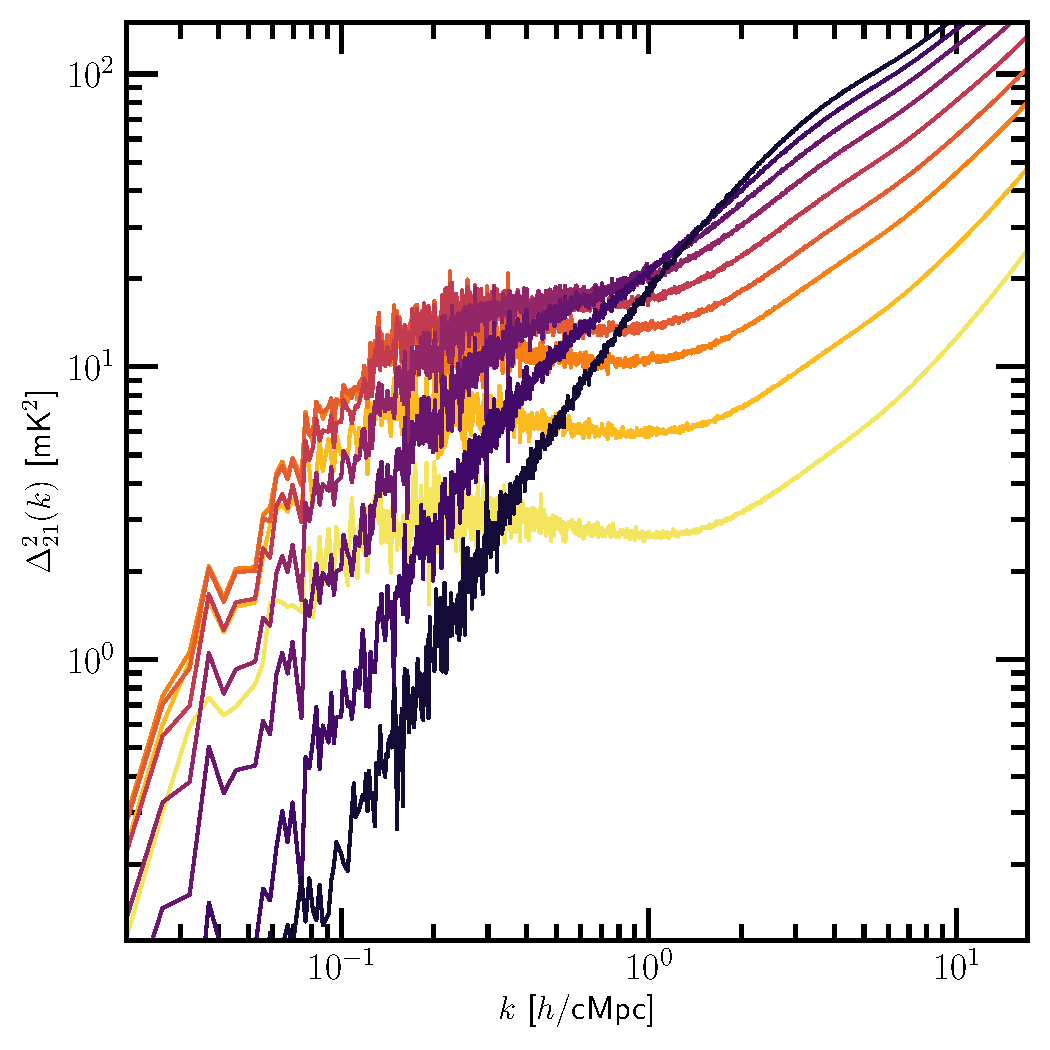
\includegraphics[width=0.99\columnwidth]{figs/21cm.pdf}
    \caption{The 21\,cm PS in increments of $\sim 0.1$ from $\sim 0.1-0.9$.}
    \label{fig:21cm}
\end{figure}

\begin{center}
    \begin{figure}[!t]
        \centering
    	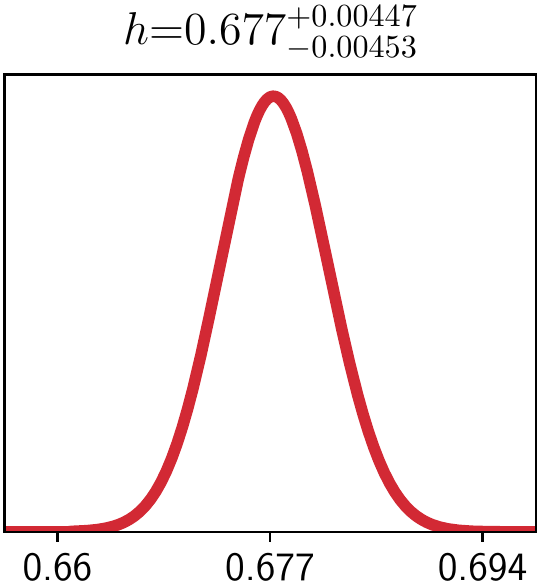
\includegraphics[scale=0.3]{figs/probdist.png}
    	\caption{Nice plot. \lipsum[11]}
        \label{fig:fig}
    \end{figure}
\end{center}


Refer to your nice figure (Fig.~\ref{fig:fig}).
\end{comment}


\section{Results}
\label{sec:result}


We begin by tracing the global (sky-averaged) evolution of the hydrogen and helium brightness temperatures, establishing the baseline thermal and ionization timeline across cosmic history. To characterize the spatial fluctuations of the ionization and brightness temperature fields, we analyze the VID (one-point), power spectrum (two-point), and bispectrum (three-point) statistics. Finally, because the peak of the power spectrum and the sign-flip transitions in the bispectrum encode characteristic spatial scales, we explicitly analyze the ionized bubble size distribution. We cross-validate these physically driven topological scales by comparing direct geometric extraction techniques, specifically, the mean-free-path method \citep[][]{Mesinger2007, Neyer2024, Neyer2026} against the statistical signatures derived from our higher-order spectra.



\begin{comment}


%\subsubsection{Dark Age}

%During the Dark Ages ($200 \gtrsim z \gtrsim 40$), prior to the formation of the first stars (thus, $x_\alpha = 0$), the 21\,cm signal is dictated primarily by the interplay between the CMB and the cooling gas. Initially, at $z \gtrsim 200$, high gas densities ensure that collisional coupling is sufficiently abundant to keep the spin temperature $T_S$ coupled to the gas kinetic temperature $T_K$.

%As the Universe expands, the gas and radiation temperatures diverge; the gas cools adiabatically as $T_K \propto (1+z)^2$, while the CMB temperature drops more slowly as $T_\gamma \propto (1+z)$. Consequently, the gas becomes significantly colder than the radiation ($T_K < T_\gamma$). This temperature gradient, maintained by collisional coupling, drives $T_S$ below $T_\gamma$, resulting in a characteristic early absorption signal ($\bar{T}_b < 0$).

%As expansion continues toward $z \approx 40$, the decreasing gas density eventually renders collisional coupling ineffective. Without this coupling, radiative transitions to the CMB dominate, forcing $T_S \to T_\gamma$. This leads to the disappearance of the detectable 21\,cm signal until the onset of Cosmic Dawn and the subsequent rise of the Ly$\alpha$ coupling. Within the \lumina simulation, we observe this transition clearly: starting from $z \approx 50$, the hydrogen spin temperature begins approaching the CMB temperature, eventually reaching thermal equilibrium ($T_S \approx T_{\gamma}$) at approximately $z \approx 30$.


%\subsubsection{Cosmic Dawn}

%The transition to Cosmic Dawn is marked by the formation of the first stars and galaxies, which initiate the growth of the Ly$\alpha$ coupling coefficient ($x_\alpha$). During this era, the spin temperature begins to decouple from the CMB and track the gas kinetic temperature ($T_S \to T_K$). Because the emissivity required for Ly$\alpha$ coupling is significantly lower than that required for X-ray heating, $T_K$ remains well below $T_\gamma$ during the early stages of this transition.

%This results in a prominent absorption dip in the 21\,cm global signal, where $T_S \approx T_K < T_\gamma$. The depth and timing of this dip in \lumina are sensitive to the specific modeling of early star formation and the efficiency of Ly$\alpha$ flux production We provide a comprehensive assessment of these model uncertainties and their impact on the cosmic timeline in Section (model dependency).  %During this period, $\delta T_b$ fluctuations are primarily driven by a combination of density variations and spatial fluctuations in the Ly$\alpha$ flux.

%As star formation accelerates, the Ly$\alpha$ coupling eventually saturates ($x_\alpha \gg 1$) at a redshift $z_\alpha$, by which point the gas throughout the IGM is strongly coupled. The timing of the $z_\alpha$ also depends on the models. As the IGM temperature rises, the signal transitions from absorption to emission. Eventually, at the heating transition redshift $z_h$, the volume-averaged kinetic temperature equals the CMB temperature ($\bar{T}_K = T_\gamma$), marking the point where the global 21\,cm signal crosses zero before entering the emission phase ($T_K > T_\gamma$). %\textcolor{red}{Also depends on the model, but usually the redshift 15-10.}


%\subsubsection{The Emission Phase and the Onset of Reionization}


%Following the heating transition ($T_K > T_\gamma$), the 21\,cm signal enters the emission regime ($\bar{T}_b > 0$). As star formation and X-ray production accelerate, the gas temperature reaches a saturation point at redshift $z_T$, where the spin temperature becomes both strongly coupled and significantly higher than the CMB temperature ($T_S \approx T_K \gg T_\gamma$). In this high-temperature limit, the brightness temperature becomes effectively independent of the exact value of $T_S$, and the signal is instead dictated by the density and ionization state of the gas.


%By this epoch, the ionization fraction ($x_i$) typically rises above the percent level, and the growth of \ion{H}{2} regions begins to accelerate. Consequently, the $\delta T_b$ fluctuations transition from being thermally driven to being dominated by the "patchiness" of reionization. As the filling fraction of these ionized bubbles becomes significant, the 21\,cm signal tracks the spatial distribution of neutral hydrogen density and the advancing ionization fronts, eventually leading to the complete depletion of the signal as reionization reaches completion.


% Post-saturation, fluctuations in the Ly$\alpha$ flux no longer influence the signal, and X-ray heating becomes the dominant driver of $T_b$ evolution.

%First star and galaxy formation, $x_a$ starts to grow, slowly $T_S$ couples to $T_K$, but still the $T_K < T_{CMB}$ so that's why we see the dip, but it depends on the model we use, because the model indicate how fast $T_S$ couples to $T_K$. Also the gas temperature at that moment influenced as well. If there's no X-ray heating then the dip should be deeper as well (just like other literatures we see) The first stars and galaxies (sources) emit both Ly$\alpha$ photons and X-rays. In general, the emissivity required for Ly$\alpha$ coupling is significantly less than that for heating $T_K$ above $T_\gamma$. In this regime, the spin temperature is coupled to cold gas so that $T_S \sim T_K < T_\gamma$. So we can expect there is an absorption signal. During this time, the temperature fluctuations are dominated by density fluctuations and variation in the Ly$\alpha$ flux. As further star formation occurs, the Ly$\alpha$ coupling will eventually saturate ($x_\alpha \gg 1$), by the redshift $z_\alpha$, the gas everywhere be strongly coupled. After Ly$\alpha$ coupling saturates, fluctuations in the Ly$\alpha$ flux no longer affect the 21\,cm signal. So the heating becomes significant, and the gas temperature fluctuation sources the $T_b$ fluctuations. When $T_K < T_\gamma$, a 21\,cm signal is seen in absorption, and $T_K > T_\gamma$, then the signal is seen in emission. Eventually at $z = z_h$, the gas will be heated everywhere, so $\bar{T}_K = T_\gamma$.


%After the heating transition, $T_K > T_\gamma$, and we expect to see a 21\,cm in emission.

%At $z_T$, when $T_S \sim T_K \gg T_\gamma$, the 21\,cm brightness temperature is saturated. The ionizing fraction has likely risen above the percent level, and $T_b$ fluctuations are sourced by a mixture of fluctuations in ionization density and gas temperature.


%\subsubsection{After Reionization}

%Following the completion of reionization, the diffuse IGM  becomes fully ionized, and the global 21\,cm signal effectively vanishes. Any residual 21\,cm emission at $z < z_{reion}$ originates primarily from "collapsed islands" of neutral hydrogen that remain shielded from the ionizing background radiation. These are largely identified as Damped Ly$\alpha$ systems (DLAs), where the high column density of gas allows hydrogen to remain neutral. Consequently, in the post-reionization epoch, the 21\,cm signal ceases to be a probe of the bulk IGM and instead becomes a tracer of the large-scale distribution of neutral gas within discrete galactic halos, serving as a key tool for 21\,cm intensity mapping studies.


\subsection{Model Variations}

Figure \ref{fig:global} will be the one with the various models. The top panel of Figure \ref{fig:global} displays the thermal evolution of the CMB photons ($T_\gamma$), the gas kinetic temperature ($T_K$), and the spin temperature ($T_S$) across a range of Ly$\alpha$ coupling efficiencies. The Ly$\alpha$ coupling coefficient ($x_\alpha$) is determined by several astrophysical factors, including the star-formation rate (SFR), the stellar spectral energy distribution (SED), and the maximum level of Lyman-series transitions included in the radiative transfer calculation.

In this study, we explore a broad parameter space by varying the star formation efficiency and employing diverse stellar population synthesis models. Specifically, we investigate the impact of different metallicities and spectral distributions to ensure our results span a realistic range of early galaxy formation scenarios. This systematic variation allows us to quantify the sensitivity of the 21\,cm signature to the fundamental properties of the first luminous sources.


Our results indicate that across all investigated models, the spin temperature effectively couples to the gas kinetic temperature by the onset of reionization $z \sim 10-15$; specifically, $T_S$ remains significantly higher than the CMB temperature during this later phase. The primary divergence between models occurs during the transition of the spin temperature from the CMB temperature to the gas kinetic temperature.

The timing of this departure and the rate at which $T_S$ thermalizes with $T_K$ are highly dependent on the choice of astrophysical parameters. Models characterized by higher SFR and lower stellar population metallicities exhibit a rapid transition from $T_\gamma$ to $T_K$. Conversely, models with lower star-formation rates and higher metallicities demonstrate a more protracted coupling phase. This behavior is driven by the enhanced production of Ly$\alpha$ photons in more active, metal-poor stellar populations, which facilitates a more rapid saturation of the Wouthuysen-Field effect.


The middle panel of Figure \ref{fig:global} presents the evolution of the 21\,cm differential brightness temperature ($\delta T_b$). The global signal mirrors the behavior of the spin temperature, exhibiting a characteristic absorption feature whose timing and depth are highly model-dependent. Similar to our findings for $T_S$, all models converge to a consistent brightness temperature during the EoR, as the signal enters the saturated emission regime ($T_S \gg T_\gamma$).

However, the models diverge significantly regarding the redshift of the absorption extrema and the total amplitude of the signal. Models incorporating higher SFR and lower-metallicity stellar populations predict a deeper absorption peak occurring at higher redshifts. This is due to the rapid establishment of the Ly$\alpha$ background, which couples $T_S$ to $T_K$ while the gas remains at its minimum adiabatic temperature. Conversely, models with lower SFR and higher metallicities shift the absorption peak to lower redshifts with a reduced amplitude, reflecting a more gradual coupling process that competes with the onset of X-ray heating.


The bottom panel of Figure \ref{fig:global} displays the global evolution of the 3.46\,cm helium hyperfine differential brightness temperature. In contrast to the hydrogen 21\,cm signal, the helium signature exhibits negligible sensitivity to the choice of astrophysical model, resulting in a uniform brightness temperature profile across all simulations. This model-independence arises because the onset of helium single-ionization ($\mathrm{He}\rightarrow \mathrm{HeII}$) occurs during the Epoch of Reionization, by which point the spin temperature has already saturated to the gas kinetic temperature ($T_S \approx T_K \gg T_\gamma$) in all scenarios. Since the brightness temperature depends primarily on the singly-ionized helium fraction ($f_{\mathrm{HeII}}$ in Eq. \ref{eq:helium}) and local overdensity rather than the nuances of the early Ly$\alpha$ background, the global evolution converges to a singular, robust prediction.

%The bottom panel of Figure \ref{fig:global} indicates the global evolution of 3.46\,cm helium differential brightness temperature. This one is not sensitive to the choice of the model, unlike the hydrogen 21\,cm signal, it shows no variations in the brightness temperature profile. It is because at the moment of single-ionized helium appears during the EoR, the spin temperature is already saturated to the gas kinetic temperature, whichever models used. And also, this brightness temperature depends not only on the spin temperature, but also the single-ionized helium fraction ($f_\mathrm{HeII}$ in Equation \ref{eq:helium}) and loca loverdensity, the global evolution shows only one result.


%The middle panel shows the hydrogen 21\,cm differential brightness temperature evolution. The brightness temperature also shows similar behavior as the spin temperature. It also shows the same brightness temperature whatever the models used during the EoR, while the model predicts differently on the moment of the absorption peak and the amount of the temperature goes down. Also, the models with higher SFR and lower metallicity stellar population models shows the deeper absorption peak at very high redshift, while the lower SFR and higher metallcity stellar population models predict the peaks at relatively lower redshift and the absorption peak is also lower.



%The first thing we found is whatever the model uses, the spin temperature is coupled to the gas kinetic temperature at the beginning of the reionization, at least the spin temperature is way higher than the CMB temperature. The difference is happening where the transition of the spin temperature from the CMB temperature to the gas kinetic temperture. The moment of deviation and how fast it is coupled to the gas temperature varies with the model we use. The models having higher star-formation rate and the lower stellar population metallicity shows the fast migration from the CMB temperature to the gas temperature, while the lower star-formation rate and the higher metallicity models show the slower transition.


%Top panel shows the temperature evolution of the CMB photons, gas kinetic temperature, and the spin temperature using various different Ly$\alpha$ coupling efficiencies. The Ly$\alpha$ coupling coefficients are determined by various factors, such as the star-formation rate, the spectral distribution function, and the energy level of Lyman series you include. For this study we varies a broad range of parameter spaces as possible, by changing different star formation efficiencies, spectral distributions using different stellar population models using different metallcities.


%Explain the global evolution. Depending on the model, the depth and the time of the dip will be different. I will show different model results. Also, note that other research limitations, they never actually used the physically consistent models, they just normalized some parameters to get the results they wanted.

\end{comment}


\subsection{Global evolution and cosmic variance} \label{sec:global}


\begin{figure*}[!t]
    \centering
    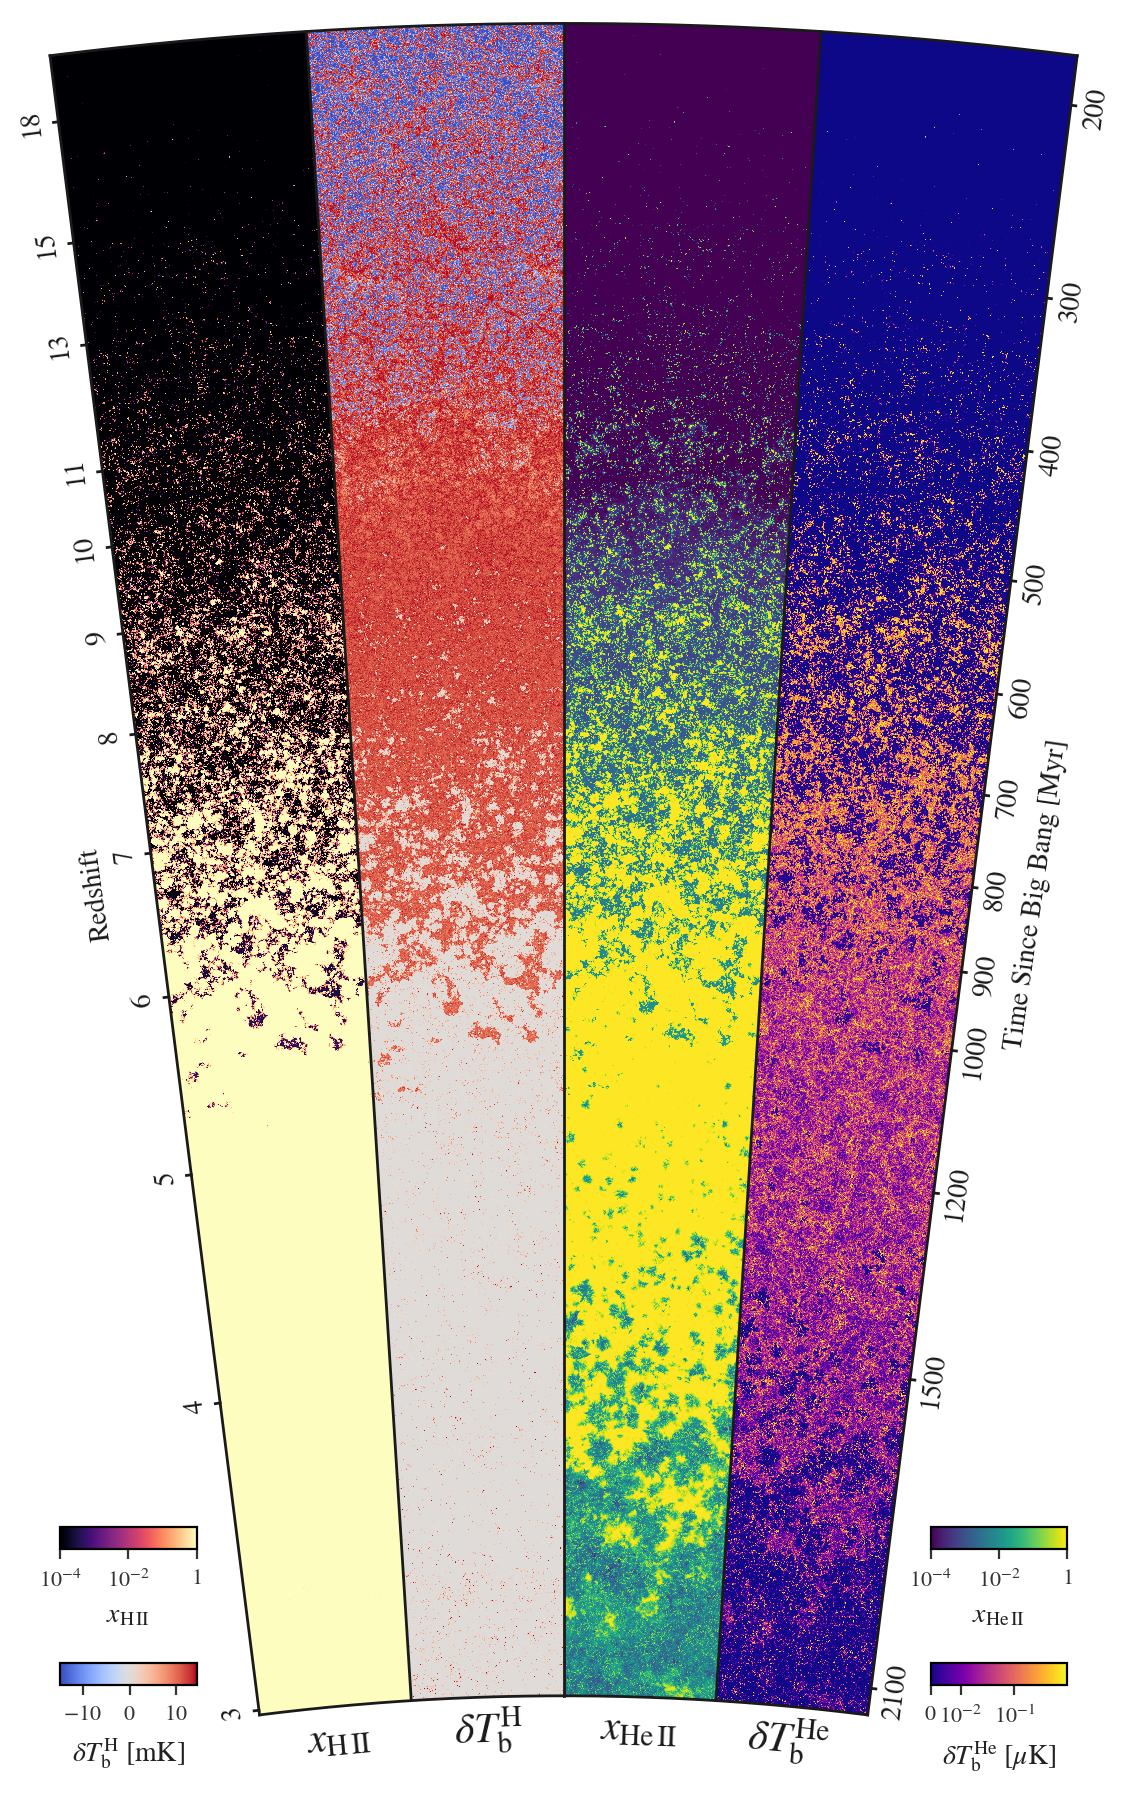
\includegraphics[width=0.80\textwidth,height=0.78\textheight,keepaspectratio]{figs/lightcone.png}
    \caption{Lightcone visualization of the simulated reionization fields, extending from $z = 20$ (outer edge) to $z = 3$ (inner edge). From left: the ionized hydrogen fraction $x_\mathrm{H\,II}$, the 21\,cm brightness temperature $\delta T_\mathrm{b}^\mathrm{H}$, the singly ionized helium fraction $x_\mathrm{He\,II}$, and the 3.46\,cm brightness temperature $\delta T_\mathrm{b}^\mathrm{He}$. The left horizontal axis marks redshift and the right axis marks cosmic age.}
    \label{fig:lightcone}
\end{figure*}

Figure \ref{fig:lightcone} presents a multi-field lightcone constructed from the \lumina simulation, spanning from $z = 20$ (roughly $180\,\mathrm{Myr}$ after the Big Bang) to $z = 3$ (roughly $2.2\,\mathrm{Gyr}$). The radial direction traces cosmic time, with decreasing redshift toward the center. The four sectors display, from left to right, the ionized hydrogen fraction $x_{\rm H\,II}$, the hydrogen 21\,cm brightness temperature $\delta T_b^{\rm H}$, the singly ionized helium fraction $x_{\rm He\,II}$, and the helium 3.46\,cm brightness temperature $\delta T_b^{\rm He}$. All fields are extracted with on-the-fly light-cone geometry, providing a unified view of the coupled ionization history of the IGM.


The $x_{\rm H\,II}$ sector shows ionized bubbles forming around overdense regions from $z \sim 13$, growing and merging following inside-out reionization until the IGM is fully ionized by $z \sim 5.2$. The $\delta T_b^\mathrm{H}$ sector traces the full thermal and ionization evolution of the 21\,cm signal. At high redshift the signal appears in absorption ($T_S < T_\gamma$), before X-ray heating from early sources raises the gas temperature above the CMB and Ly$\alpha$ coupling drives $T_S$ toward $T_K$, transitioning the signal into emission. The subsequent growth and percolation of \ion{H}{2} regions imprints a characteristic large-scale patchiness on the emission field, which progressively suppresses the signal until it vanishes as hydrogen reionization completes near $z \sim 5.5$. The $\delta T_b^\mathrm{He}$ sector reveals filamentary structure tracing the underlying matter distribution, while the $x_\mathrm{He\,II}$ sector shows \ion{He}{3} bubbles carved by the hard ionizing spectra of quasars at $z \sim 3$--$5$. Notably, while hydrogen reionization is essentially complete by $z \sim 5.5$, the helium sectors continue to evolve at lower redshifts, capturing a secondary reionization epoch inaccessible to 21\,cm observations alone.


%Figure \ref{fig:lightcone} presents a multi-field lightcone constructed from the \lumina simulation, spanning from $z =  20$ (roughly $180\,\mathrm{Myr}$ after the Big Bang) to $z = 3$ (roughly $2.2\,\mathrm{Gyr}$). The radial direction traces cosmic time, with decreasing redshift toward the center, while each quadrant shows a distinct physical field extracted from the same underlying simulation volume. Proceeding clockwise from the top left, the four quadrants show the ionized hydrogen fraction $x_\mathrm{H\,II}$, the 21\,cm brightness temperature $\delta T_\mathrm{b}^\mathrm{H}$, the 3.46\,cm brightness temperature $\delta T_\mathrm{b}^\mathrm{He}$, and the singly ionized helium fraction $x_\mathrm{He\,II}$.


%This picture presents a unified view of the coupled ionization history of the IGM across both reionization epochs. Because this polar layout maps a flat simulation slice onto a circular wedge, the physical dimensions are inherently distorted. Specifically, the azimuthal arc of each 90-degree quadrant spans the full $500\,\mathrm{cMpc}$ transverse width of the simulation box. Consequently, the transverse spatial scale is visually stretched at high redshifts (outer radii) and compressed at low redshifts (inner radii). Additionally, the radial axis is compressed relative to this transverse scale, mapping the entire redshift range from $z = 20$ down to $z = 3$ into the radial depth of the plot.




%The two halves of the lightcone capture two distinct reionization epochs, separated in redshift and driven by different source populations. In the upper half, the $x_\mathrm{H\,I}$ field transitions from a nearly neutral IGM at high redshift to a fully ionized medium by $z \sim 5$, with ionized regions initially confined to the most overdense environments before expanding and percolating into the surrounding voids, which is a visual manifestation of the inside-out reionization topology. The corresponding $\delta T_\mathrm{b}^\mathrm{H}$ field traces this evolution as a progressive suppression of the 21\,cm signal across increasingly large contiguous regions. In the lower half, the $x_\mathrm{He\,II}$ field captures the helium reionization history: helium is first singly ionized by the soft stellar UV that also drives hydrogen reionization, so the He\,II fraction builds up from $z \sim 10$ and reaches its maximum near $z \sim 6$--5, before the hard, non-stellar spectra of quasars and AGN doubly ionize helium to He\,III over $z \sim 5$--3, depleting the He\,II fraction. The $\delta T_\mathrm{b}^\mathrm{He}$ field correspondingly reveals the He\,II gas as bright shells surrounding the growing He\,III bubbles carved out by these hard sources.


\begin{figure}[!t]
    \centering
    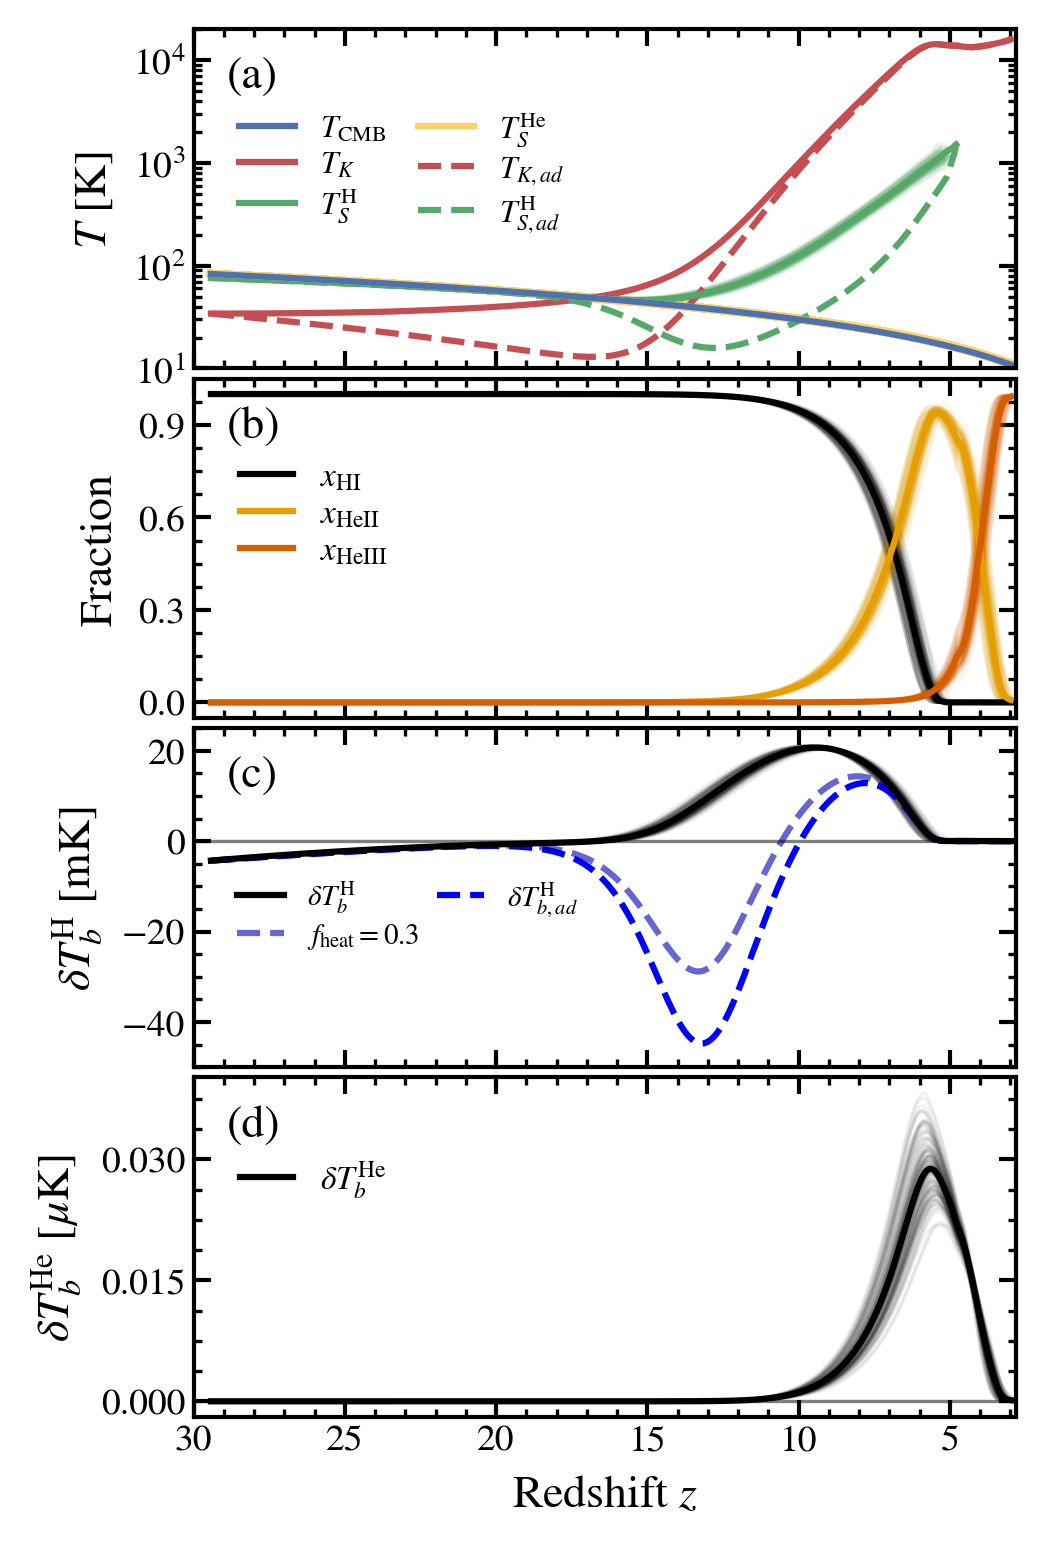
\includegraphics[width=\linewidth]{figs/global.png}
    \caption{Global thermal and ionization history in the \lumina simulation from $z = 30$ to $z = 3$. Bold solid curves show the volume-weighted global average across the 500\,cMpc volume, while faint background curves trace 125 non-overlapping 100\,cMpc sub-volumes to illustrate cosmic variance. The blue dashed curves show the post-processed adiabatic reference.  (a) Redshift evolution of $T_\mathrm{CMB}$, gas kinetic temperature $T_K$, and spin temperatures $T_\mathrm{S}^\mathrm{H}$ and $T_\mathrm{S}^\mathrm{He}$. Note that $T_\mathrm{S}^\mathrm{He}$ (yellow) tightly tracks $T_\mathrm{CMB}$ (blue) throughout. (b) Global ionization fractions for neutral hydrogen ($x_\mathrm{H\,I}$), singly ionized helium ($x_\mathrm{He\,II}$), and doubly ionized helium ($x_\mathrm{He\,III}$). (c) 21\,cm differential brightness temperature $\delta T_\mathrm{b}^\mathrm{H}$, including an interpolation between the fiducial and adiabatic signals ($f_\mathrm{heat}\,\delta T_b^\mathrm{H} + (1-f_\mathrm{heat})\,\delta T_{b,\mathrm{ad}}^\mathrm{H}$, where $f_\mathrm{heat} = 0.3$), and the adiabatic reference $\delta T_{\mathrm{b},\mathrm{ad}}^\mathrm{H}$. (d) 3.46\,cm brightness temperature $\delta T_\mathrm{b}^\mathrm{He}$, highlighting the delayed emission peak and its subsequent suppression during \ion{He}{3} reionization.}
    \label{fig:global}
\end{figure}

% an interpolation between the fiducial and adiabatic signals, $f\,\delta T_b^\mathrm{H} + (1-f)\,\delta T_{b,\mathrm{ad}}^\mathrm{H}$, labelled by $f_\mathrm{heat}$


Figure \ref{fig:global} presents the global thermal and ionization history of the \lumina simulation, computed as the volume-weighted average across the full 500\,cMpc box. This global average provides a robust reference for the epochs of both hydrogen and helium reionization, capturing the mean evolutionary trajectory while averaging over local environmental fluctuations.


Reionization is, however, inherently inhomogeneous, driven by the clustered nature of early luminous sources. To quantify the impact of this inhomogeneity, we subdivide the volume into 125 non-overlapping sub-volumes of $100\,\mathrm{cMpc}$, whose individual tracks are shown as faint shaded lines in Figure \ref{fig:global}. The spread among these tracks provides a direct measure of cosmic variance at $100\,\mathrm{cMpc}$ scales, quantifying how representative the global average is across different large-scale environments and illustrating the degree to which local source populations drive regional variations in the reionization history.


The thermal history (Figure \ref{fig:global} (a)) governs the evolution of the hyperfine signals for both hydrogen and helium, but in different ways. At high redshifts ($z \gtrsim 27$), prior to the formation of the first luminous sources, the gas kinetic temperature $T_K$ cools adiabatically below the CMB temperature $T_\gamma$. Because collisional coupling to the rarefying gas has already become inefficient and no Ly$\alpha$ background yet exists to drive Wouthuysen--Field coupling, the hydrogen spin temperature $T_S^\mathrm{H}$ decouples from $T_K$ and relaxes to $T_\gamma$ through radiative coupling to the CMB.


As the first stars and galaxies form, the growing Ly$\alpha$ background drives $T_S^\mathrm{H}$ toward $T_K$ via the Wouthuysen--Field effect, while X-ray emission from early sources drives $T_K$ above $T_\gamma$ by $z \approx 17$. The role of X-ray heating is shown directly by the adiabatic reference curves ($T_{K,\mathrm{ad}}$ and $T_{S,\mathrm{ad}}^\mathrm{H}$, dashed). The adiabatic reference assigns $T_K \propto (1+z)^2$, anchored to the simulated temperature at $z \approx 29$, only to highly neutral cells ($x_\mathrm{H\,II} < 10^{-3}$); cells already partially ionized or warmed by X-rays keep their simulated temperature. It therefore approximates the no-heating limit only at $z \gtrsim 13$, and its later rise into emission reflects this partial re-heating rather than an unheated IGM.


This post-processed benchmark is an approximation, as two competing effects distinguish it from a self-consistent run without X-ray heating near $z \sim 13$. On one hand, shock heating and compression during structure formation warm the gas and shallow the absorption trough. On the other hand, colder gas recombines more rapidly, boosting the neutral fraction and deepening the trough. Because we do not determine the net direction of these corrections, this dashed curve represents an approximate baseline rather than a strict bound. Nevertheless, it effectively isolates the impact of X-ray heating: contrasting this reference with our fiducial model reveals that efficient heating is strong enough to completely suppress the expected absorption feature. A direct no X-ray heating simulation is deferred to future work.

% We compute the adiabatic limit in post-processing by isolating highly neutral gas within the simulation ($x_{\rm HII} < 10^{-3}$). We then analytically evolve its thermal history by enforcing the cosmological expansion cooling rate, $T_K \propto (1+z)^2$, anchored to a high-redshift reference point prior to the onset of X-ray heating. This construction is an approximation as two competing effects on $\delta T^\mathrm{H}_b$ would distinguish it from a self-consistent no-X-ray-heating run near $z \sim 15$.

By $z \lesssim 12$, the morphological evolution of the 21\,cm signal is overwhelmingly governed by the ionization state of the IGM. In our fiducial run, the gas has heated above the CMB temperature ($T_S^\mathrm{H} \gg T_\gamma$), approaching the thermally saturated emission regime. The hydrogen brightness temperature becomes insensitive to further thermal evolution, and the late-time signal is set almost entirely by the topology of the expanding \ion{H}{2} regions.

%By $z \lesssim 10$ both $T_K$ and $T_S^\mathrm{H}$ have risen well above $T_\gamma$, reaching the thermally saturated regime ($T_S^\mathrm{H} \gg T_\gamma$) in which the hydrogen brightness temperature becomes insensitive to further thermal evolution and is governed primarily by the ionization state of the IGM.


The helium spin temperature behaves differently. In the global average $T_S^\mathrm{He}$ remains almost pinned to $T_\gamma$ throughout, not coupling to the much hotter gas as $T_S^\mathrm{H}$ does. This reflects the intrinsic weakness of both coupling channels for the $^{3}\mathrm{He}^{+}$ 3.46\,cm transition. Its spontaneous-decay rate exceeds that of the 21\,cm line by a factor of 690 ($A^\mathrm{He}_{10} \gg A^\mathrm{H}_{10}$), and the \ion{He}{2} Ly$\alpha$ (40.8 eV) background that would drive helium Wouthuysen--Field coupling is weaker than its hydrogen counterpart, so both the radiative and collisional coupling coefficients remain $\ll 1$ on average. With $T_S^\mathrm{He} \simeq T_\gamma$, the factor $(1 - T_\gamma/T_S^\mathrm{He})$ nearly vanishes, foreshadowing the strongly suppressed helium signal discussed below.



The global neutral hydrogen fraction $x_\mathrm{H\,I}$ (Figure \ref{fig:global} (b)) directly traces the ionization history of hydrogen reionization. At high redshifts ($z \gtrsim 12$) the IGM remains overwhelmingly neutral, $x_\mathrm{H\,I} \approx 1$, as the ionizing photon budget from the stellar populations is insufficient to overcome the high recombination rate of the dense early IGM. As galaxy formation accelerates and the ionizing output grows, $x_\mathrm{H\,I}$ begins to decline rapidly around $z \sim 9$--$10$, reflecting the emergence and expansion of isolated \ion{H}{2} regions around luminous sources concentrated in the most overdense environments of the cosmic web. As these regions grow and overlap, the decline accelerates, with large-scale percolation driving the rapid completion of reionization by $z \approx 5.5$--$6$, consistent with constraints from quasar absorption spectra, the Lyman-$\alpha$ forest opacity, and the dark-pixel and dark-gap statistics \citep[e.g.][]{McGreer2015, Bosman2022, Zhu2022}. The sub-volume spread during the rapid decline confirms the inhomogeneous nature of reionization: overdense regions, which host more abundant and luminous sources, transition earlier than underdense voids, producing the characteristic scatter visible in Figure \ref{fig:global} (b).



Panel (b) of Figure \ref{fig:global} also details the evolution of helium ionization states ($x_\mathrm{He\,II}$ and $x_\mathrm{He\,III}$). At high redshifts ($z \gtrsim 10$) helium remains predominantly neutral, as the soft UV photons driving hydrogen reionization lack the energy to ionize helium. As stellar populations build a widespread ionizing background, $x_\mathrm{He\,II}$ rises to a peak of $\sim 0.93$ around $z \approx 5$--$6$, when singly ionized helium temporarily dominates the IGM. Concurrently, the growing population of quasars and AGN drives the rise of $x_\mathrm{He\,III}$. Their hard spectra carry sufficient energy to doubly ionize helium, and $x_\mathrm{He\,III}$ crosses $x_\mathrm{He\,II}$ around $z \approx 4$, marking the point at which \ion{He}{3} becomes the dominant state. Beyond this crossing $x_\mathrm{He\,II}$ declines rapidly as the remaining \ion{He}{2} is consumed by the intensifying quasar field, while $x_\mathrm{He\,III}$ rises toward unity. Both curves exhibit sub-volume scatter comparable to the hydrogen fields, reflecting the inhomogeneous distribution of quasar sources: overdense sub-volumes host more abundant quasar activity and undergo the \ion{He}{2}--\ion{He}{3} transition earlier than underdense ones.


The global 21\,cm brightness temperature $\delta T_b^\mathrm{H}$ (Figure \ref{fig:global} (c)) is shaped by the interplay between the thermal history (panel a) and the ionization history (panel b), with each dominating at different epochs. At high redshifts ($z \gtrsim 18$), prior to efficient X-ray heating, $T_K < T_\gamma$ and the signal appears in a brief, shallow absorption before heating dominates. As X-ray heating drives $T_K$ above $T_\gamma$ and Ly$\alpha$ coupling saturates ($T_S^\mathrm{H} \gg T_\gamma$), the signal transitions into emission and rises while the neutral fraction remains high, peaking at $\sim 20\ \mathrm{mK}$ around $z \approx 10$. Beyond this peak the accelerating decline of $x_\mathrm{H\,I}$ becomes the dominant driver: as \ion{H}{2} regions expand and percolate, the emission is progressively suppressed, falling to near zero by $z \approx 5.5$--$6$ as reionization completes. We caution that the absence of a deep absorption trough reflects the strong X-ray heating adopted in \lumina. As discussed below and quantified in Section \ref{sec:xray_heating}, this heating is likely too efficient, so the absence of an absorption epoch should be regarded as model-dependent. The divergence among sub-volume tracks during the emission and suppression phases reflects the inhomogeneous, inside-out progression of reionization. Overdense sub-volumes transition earlier than underdense ones, illustrating the sensitivity of the 21\,cm signal to large-scale environmental variations. The $500\,\mathrm{cMpc}$ \lumina volume is uniquely positioned to capture these variations.


The adiabatic reference signal $\delta T_{b,\mathrm{ad}}^\mathrm{H}$ (blue dashed line in Figure \ref{fig:global} (c)) isolates the impact of X-ray heating on the observable signal. Without X-ray heating, the post-processed reference develops an absorption trough of $\sim -45\ \mathrm{mK}$ near $z \approx 13$, the canonical Cosmic Dawn sequence in which Ly$\alpha$ coupling precedes X-ray heating \citep[see][]{Furlanetto2006, Pritchard2012}. The fiducial \lumina run ($f_\mathrm{heat} = 1.0$) produces no such feature, as efficient heating raises $T_K$ above $T_\gamma$ before or concurrently with Ly$\alpha$ coupling, producing the near-simultaneous or slightly reversed ordering ($z_h \gtrsim z_\alpha$) discussed in Section \ref{sec:times}. The depth of the absorption trough is thus a sensitive probe of early X-ray energy deposition. We stress, however, that the absence of an absorption feature in \lumina is in part an artifact of our energy-deposition scheme, which converts all absorbed X-ray energy into heat ($f_\mathrm{heat} = 1$). A self-consistent energy partition \citep[e.g.][]{Shull1985, Furlanetto2010} deposits only a fraction of absorbed X-ray energy as heat in the neutral IGM, delaying the $T_K = T_\gamma$ crossing. An interpolation between the two limits ($f_\mathrm{heat}=0.3$) illustrates the intermediate regime; because $\delta T_b$ is concave in $T_K$, a self-consistent calculation at reduced heating efficiency would produce weaker absorption than these interpolations. Whether a trough survives is therefore set by the heating efficiency, which we examine further in Section \ref{sec:xray_heating}.





The global 3.46\,cm brightness temperature $\delta T_b^\mathrm{He}$ (Figure \ref{fig:global} (d)) evolves in a qualitatively distinct manner from the 21\,cm signal.  Its shape closely follows the singly ionized helium fraction $x_\mathrm{He\,II}$ (panel b), rising to a peak of $\approx 0.03\ \mu\mathrm{K}$ near $z \approx 5.5$ and falling to near zero by $z \approx 3$ as the quasar radiation field converts the remaining \ion{He}{2} into \ion{He}{3}. This tracking of $x_\mathrm{He\,II}$ does not, however, arise from thermal saturation. Although the gas is hot throughout helium reionization ($T_K \gg T_\gamma$ for $z \lesssim 6$), the helium spin temperature does not thermalize to it: as shown in panel (a), the weak \ion{He}{2} Ly$\alpha$ and collisional coupling of the $^{3}\mathrm{He}^{+}$ transition leave $T_S^\mathrm{He}$ only marginally above $T_\gamma$. The thermal factor $(1 - T_\gamma/T_S^\mathrm{He})$ is therefore small and nearly constant. It sets the suppressed overall amplitude of the signal, while the shape is governed primarily by $x_\mathrm{He\,II}$. This weak coupling is precisely why the global signal reaches only $\approx 0.03\ \mu\mathrm{K}$, well below the $\sim 1\ \mu\mathrm{K}$ level obtained in the fully coupled limit $T_S^\mathrm{He} \to T_\mathrm{gas}$ \citep[][]{Khullar2020, Basu2026}. The sub-volume scatter in $\delta T_b^\mathrm{He}$ is stronger than that of the 21\,cm signal, reflecting the cosmic variance imposed by the inhomogeneous distribution of quasar sources across large-scale environments.



\begin{comment}


\subsubsection{Sub-volume Analysis and Environmental Effects}

To investigate the impact of cosmic variance and local environmental fluctuations on the 21\,cm and 3.46\,cm signals, we subdivide the primary $500^3$\,cMpc$^3$ \lumina volume into 125 independent sub-volumes of $100^3$\,cMpc$^3$ each. This multi-scale approach serves two primary purposes.

First, it allows for a rigorous quantification of the statistical uncertainty in the global signal, providing a measure of how representative the volume-averaged evolution is across different spatial scales. Second, by treating each 100\,cMpc sub-box as a distinct realization of the IGM, we can probe the correlation between the 21\,cm and 3.46\,cm signatures and the local matter overdensity. Since reionization is inherently an inhomogeneous process driven by the clustering of early sources, this decomposition is essential for understanding the transition from the large-scale global average to the patchy, scale-dependent fluctuations observed in the power spectrum.
In Figure \ref{fig:local}, we present the results from the subdivision of the \textit{LUMINA} volume into 125 independent $100^3$\,cMpc$^3$ sub-boxes. The structure mirrors Figure \ref{fig:global}, but highlights the role of cosmic variance and local environmental effects.

The upper panel shows the thermal evolution of $T_\gamma$, $T_K$, and $T_S$ across these sub-volumes. While the general cooling and coupling trends remain consistent with the global average, we observe a significant spread in the timing of the $T_S \to T_K$ transition. This variance is driven by the inhomogeneous distribution of the first luminous sources; overdense sub-volumes with accelerated star formation exhibit earlier Ly$\alpha$ coupling compared to underdense voids.

The middle panel illustrates the resulting hydrogen 21\,cm differential brightness temperature. Here, the "patchiness" of Cosmic Dawn is most evident. Depending on the local star formation efficiency and metallicity, individual sub-volumes exhibit absorption peaks at varying redshifts and depths. This scatter demonstrates that an observer focusing on a single 100\,cMpc field of view might detect an absorption signal that deviates substantially from the theoretical global average, emphasizing the necessity of large-volume surveys to mitigate sample variance.

In contrast, the bottom panel displays the 3.46\,cm helium signal, which remains remarkably robust across all sub-volumes. Even at these smaller scales, the helium brightness temperature curves are nearly overlapping, forming a singular, tight profile. This confirms that by the time helium ionization begins, the IGM has reached a state of thermal saturation where local variations in the radiation background no longer significantly alter the hyperfine signal.

\begin{figure}[!t]
    \centering
    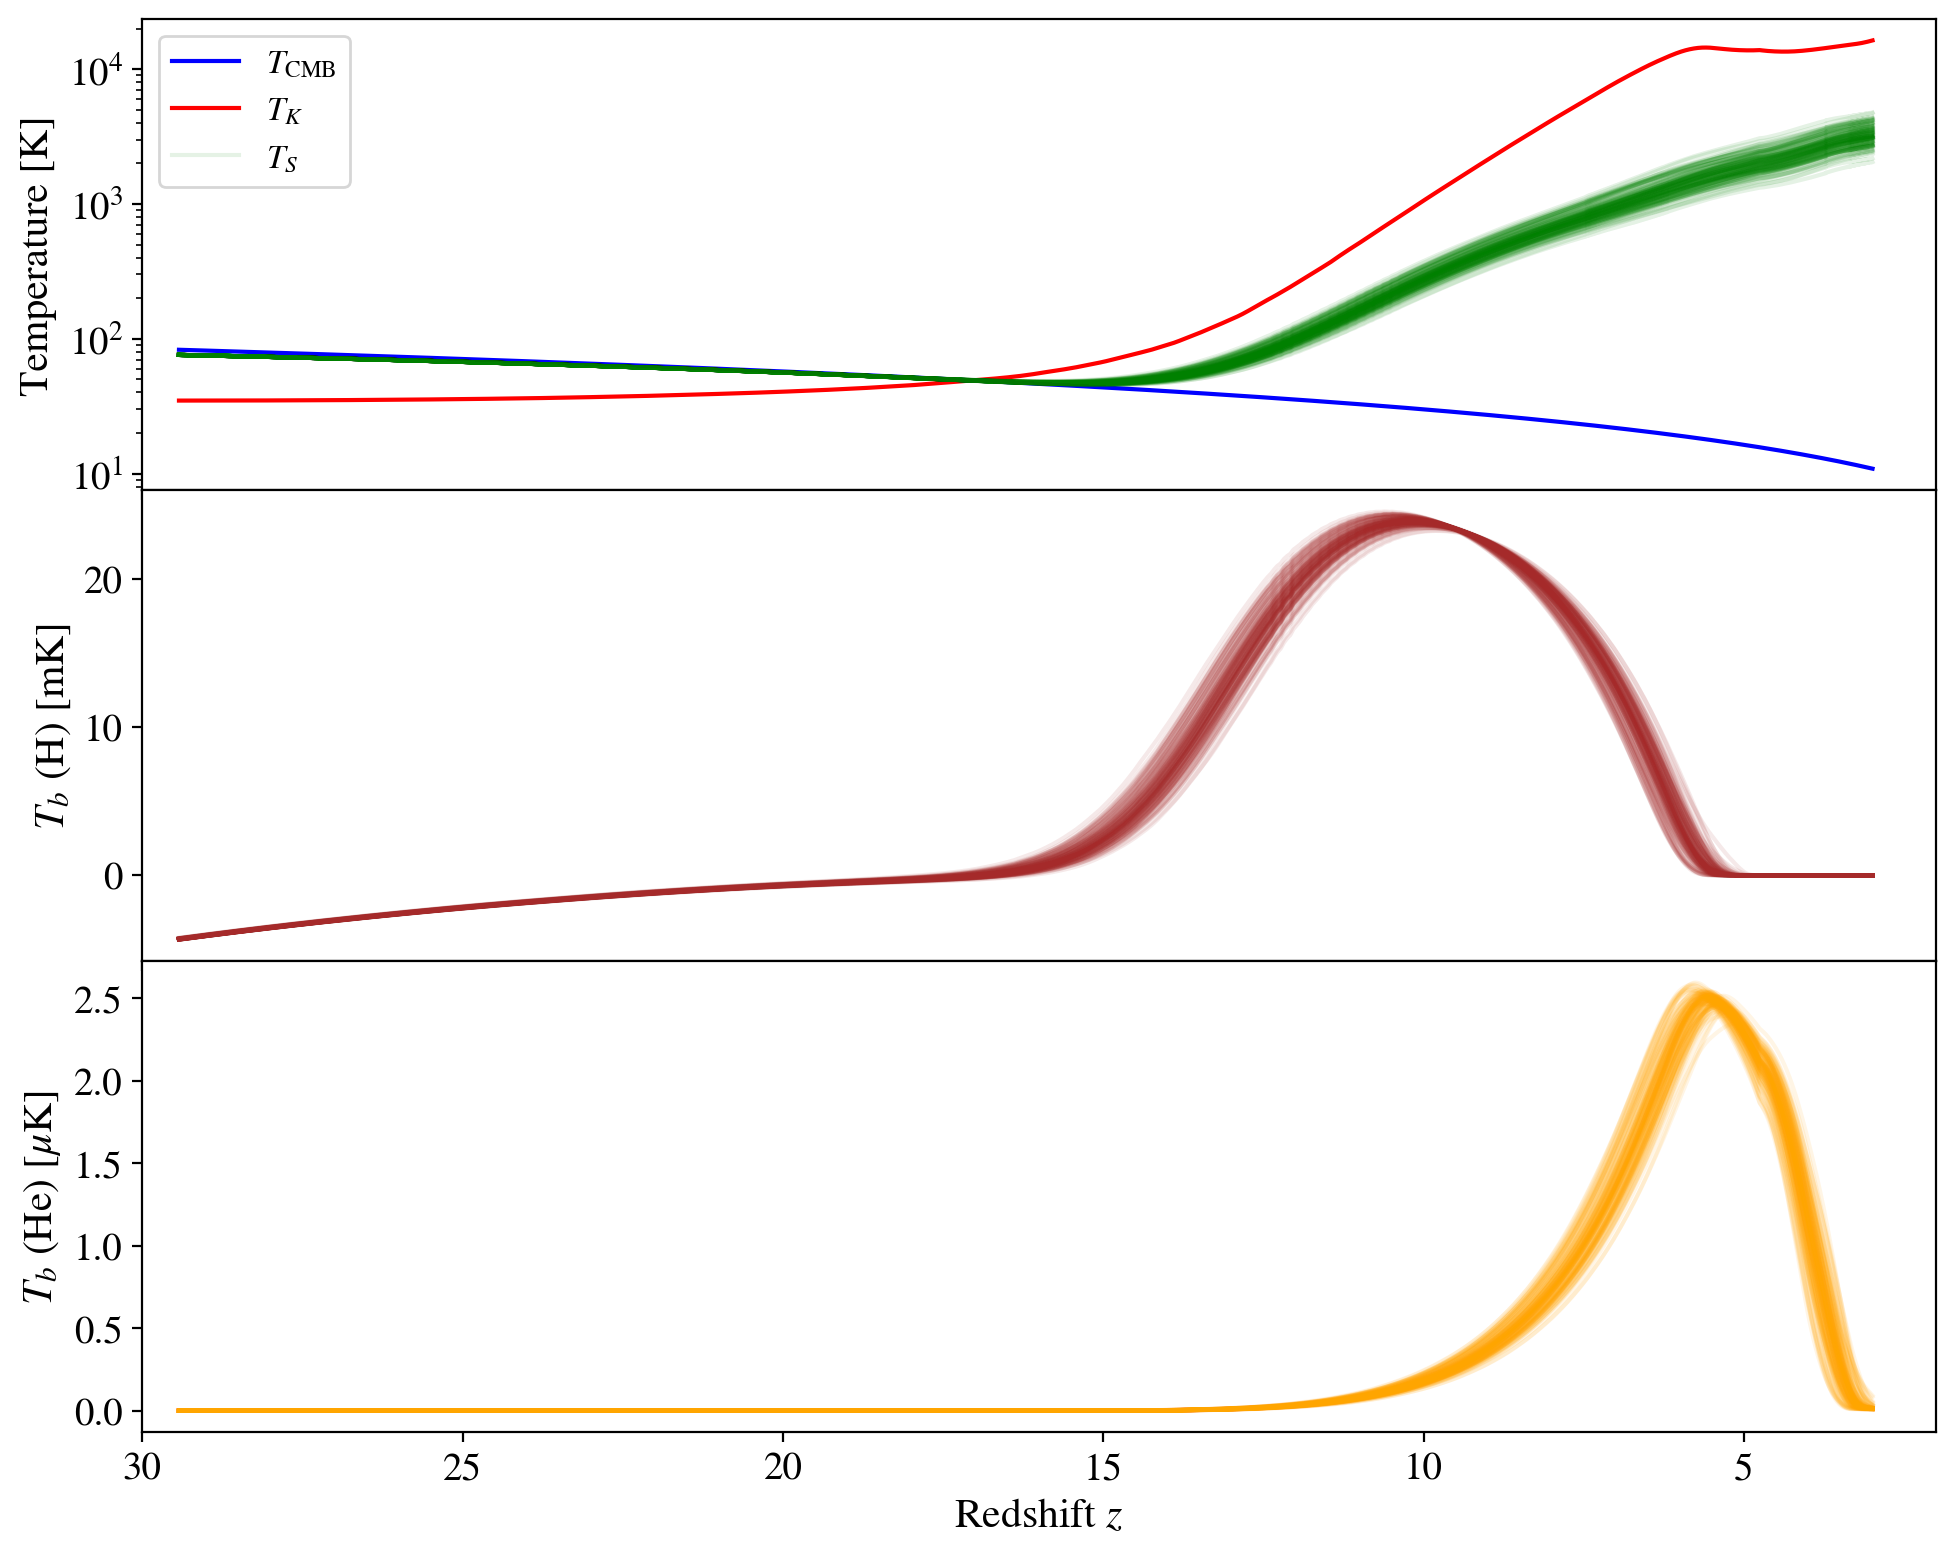
\includegraphics[width=0.47\textwidth]{figs/local.png}
    \caption{Local variations and cosmic variance across 100\,cMpc sub-volumes.
    Each panel displays results from 125 independent sub-volumes ($100^3$\,cMpc$^3$) extracted from the primary \lumina box.
    \textit{Top panel}: Thermal evolution showing the spatial scatter in the timing of $T_S$ decoupling from $T_\gamma$, driven by local density variations.
    \textit{Middle panel}: The 21\,cm differential brightness temperature, illustrating the significant "patchiness" in the absorption dip and the diversity of local reionization histories.
    \textit{Bottom panel}: The 3.46\,cm helium hyperfine signal, demonstrating its robustness and minimal sensitivity to local environmental fluctuations compared to the hydrogen signal. The spread between curves quantifies the cosmic variance inherent in small-volume 21\,cm observations.}
    \label{fig:local}
\end{figure}
\end{comment}


\begin{figure*}[!t]
    \centering
    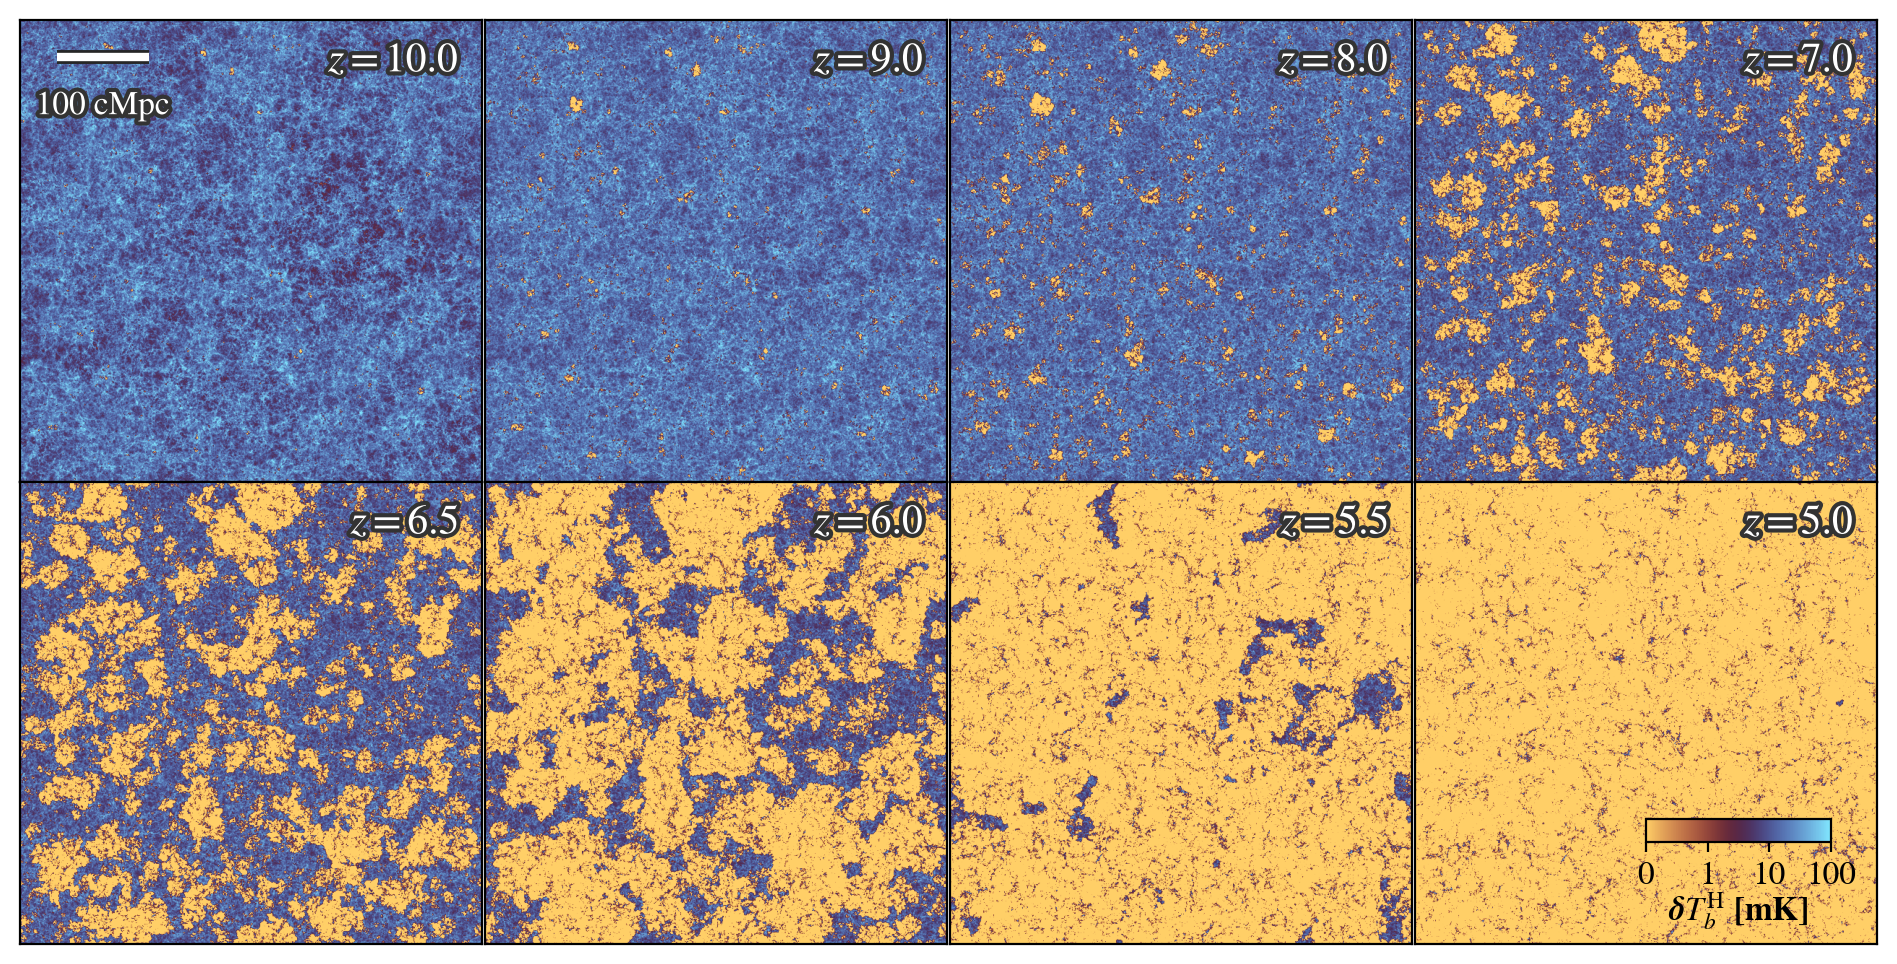
\includegraphics[width=\textwidth]{figs/tmap_hydro.png}
    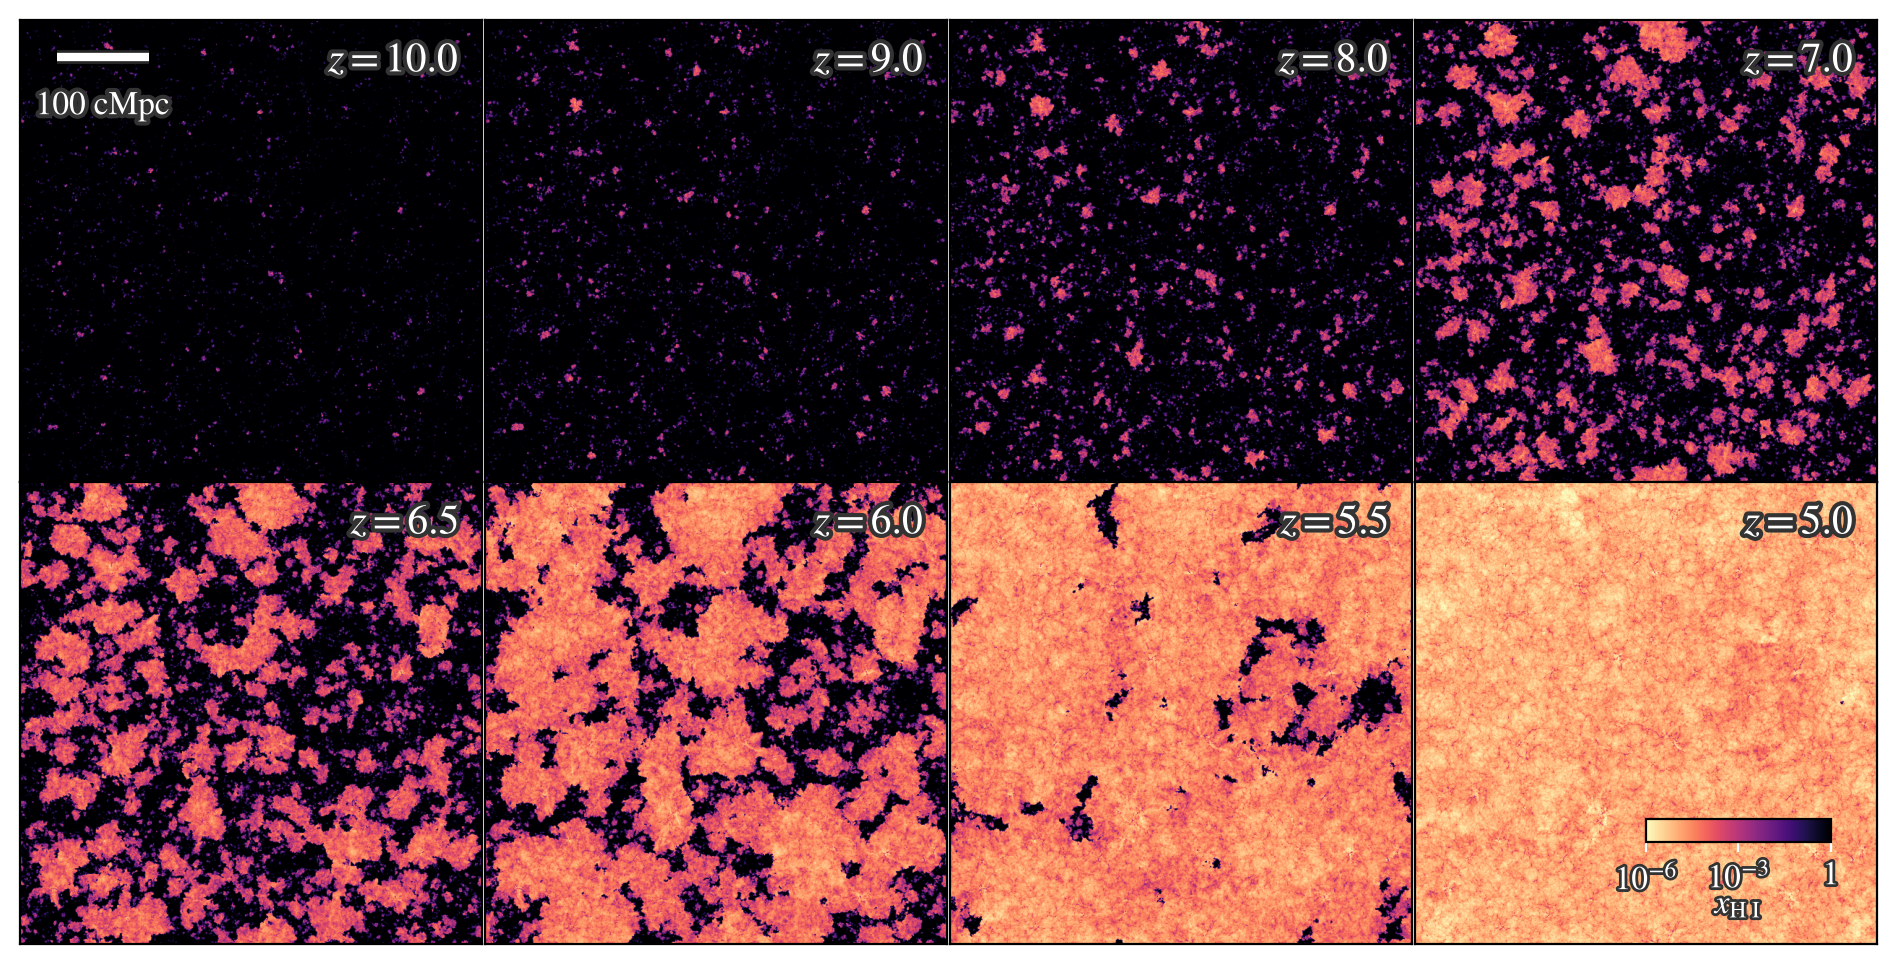
\includegraphics[width=\textwidth]{figs/f_hydro.png}
    \caption{Spatial evolution of the hydrogen 21\,cm brightness temperature, $\delta T^\mathrm{H}_\mathrm{b}$ (top panels), and the neutral hydrogen fraction, $x_\mathrm{H \,I}$ (bottom panels), from $z=10$ to $z=5$ within a $500 \, \mathrm{cMpc}$ \lumina volume.}
    \label{fig:tmap_hydro}
\end{figure*}

\subsection{Voxel intensity distribution (VID)} \label{sec:vid}


During the cosmic Dark Ages, the 21\,cm signal is primarily driven by primordial density fluctuations and follows a nearly Gaussian distribution. As luminous sources emerge, however, X-ray heating and patchy reionization introduce strongly non-Gaussian structures into the IGM. While two-point statistics such as the power spectrum are essential for quantifying scale-dependent fluctuations, they are inherently insensitive to the underlying distribution of brightness temperatures. To capture this evolving morphology, the VID serves as a complementary one-point statistical tool. By directly measuring the probability distribution function (PDF) of voxel intensities, the VID preserves information about the asymmetry and phase structure of the 21\,cm and 3.46\,cm fields that is not retained in the power spectrum alone \citep{Breysse2017, Sabla2024}. Throughout this section, the VID is computed from the noiseless, fully sampled simulation volume; Section~\ref{sec:foreground} discusses the observational challenges of recovering this one-point statistic from real interferometric data.


Despite its theoretical utility, the VID is particularly sensitive to cosmic variance in its non-Gaussian tails. In restricted simulation volumes, a small number of large ionized regions can disproportionately distort the PDF, making it unrepresentative of the global IGM. Consequently, robust measurement of the higher-order VID moments requires large cosmological volumes. By resolving the IGM across a 500\,cMpc volume, \lumina provides the statistical baseline needed to construct representative, variance-limited VIDs for both hydrogen and helium reionization. We discuss this box-size dependence in Section \ref{sec:box}, where we show that the sub-volume scatter is confined to the rare-structure tails.


To interpret the VID physically, it is useful to relate its statistical moments to the evolving phase structure of the IGM. The PDF evolves from a relatively continuous, near-Gaussian distribution at early times to one increasingly dominated by a strong zero-signal component as ionized regions expand and merge. The variance (second moment) traces the overall amplitude of fluctuations and generally decreases as the emitting neutral gas is progressively ionized. The higher-order moments probe the non-Gaussian structure of the signal directly. A Gaussian field has zero skewness and zero excess kurtosis, so any departure measures the degree of non-Gaussianity, and the progressive growth of both moments through reionization quantifies the increasingly non-Gaussian morphology of the IGM. The skewness (third moment) captures the asymmetry between the ionized and neutral phases, growing as the field separates into a dominant zero-signal component and a one-sided emitting tail. The kurtosis (fourth moment) captures the heaviness of that tail, rising as the signal becomes concentrated into rare, isolated emitting structures. Because the skewness and kurtosis are the real-space, configuration-integrated counterparts of the bispectrum, they provide a compact statistical description of the evolving IGM morphology beyond what the power spectrum alone can capture.


\subsubsection{Hydrogen VID statistics}



The spatial evolution of the 21\,cm brightness temperature, $\delta T^\mathrm{H}_\mathrm{b}$, and the neutral hydrogen fraction is illustrated in Figure~\ref{fig:tmap_hydro}, spanning the EoR from $z=10$ to $z=5$. The simulated volume extends 500\,cMpc on a side, with the visualized slices having a depth of $\sim 0.8$\,cMpc. The upper panels show the evolution of the 21\,cm brightness temperature, while the lower panels present the corresponding neutral hydrogen fraction.


At early times ($z \gtrsim 9$), the IGM remains predominantly neutral, and fluctuations in the 21\,cm signal are driven primarily by the underlying matter density field, with additional modulation from spatial variations in the gas kinetic temperature. Consequently, the signal broadly traces the large-scale cosmic web. As the first generations of galaxies form within massive dark matter halos, localized \ion{H}{2} regions begin to emerge. In the 21\,cm brightness temperature maps, these fully ionized bubbles appear as expanding zero-signal regions ($\delta T^\mathrm{H}_\mathrm{b} \approx 0$ mK, shown in yellow). Comparing the upper and lower panels reveals a direct morphological correspondence: the growth of ionized regions determines the topology of the suppressed 21\,cm signal. As star formation increases and ionizing photons escape into the IGM, these isolated bubbles expand, merge, and eventually percolate across the volume. By the end of hydrogen reionization ($z \lesssim 5.5$), most of the IGM is highly ionized, and the 21\,cm signal is extinguished across the majority of the volume, surviving only within compact, dense neutral islands and filaments.


This evolving contrast between bright neutral regions and expanding ionized voids directly shapes the VID. In particular, the progressive separation between zero-signal ionized regions and high-emission neutral gas drives the increasing bimodality and skewness of the brightness temperature distribution, making the VID a sensitive probe of reionization topology.


\begin{figure}[!t]
    \centering
    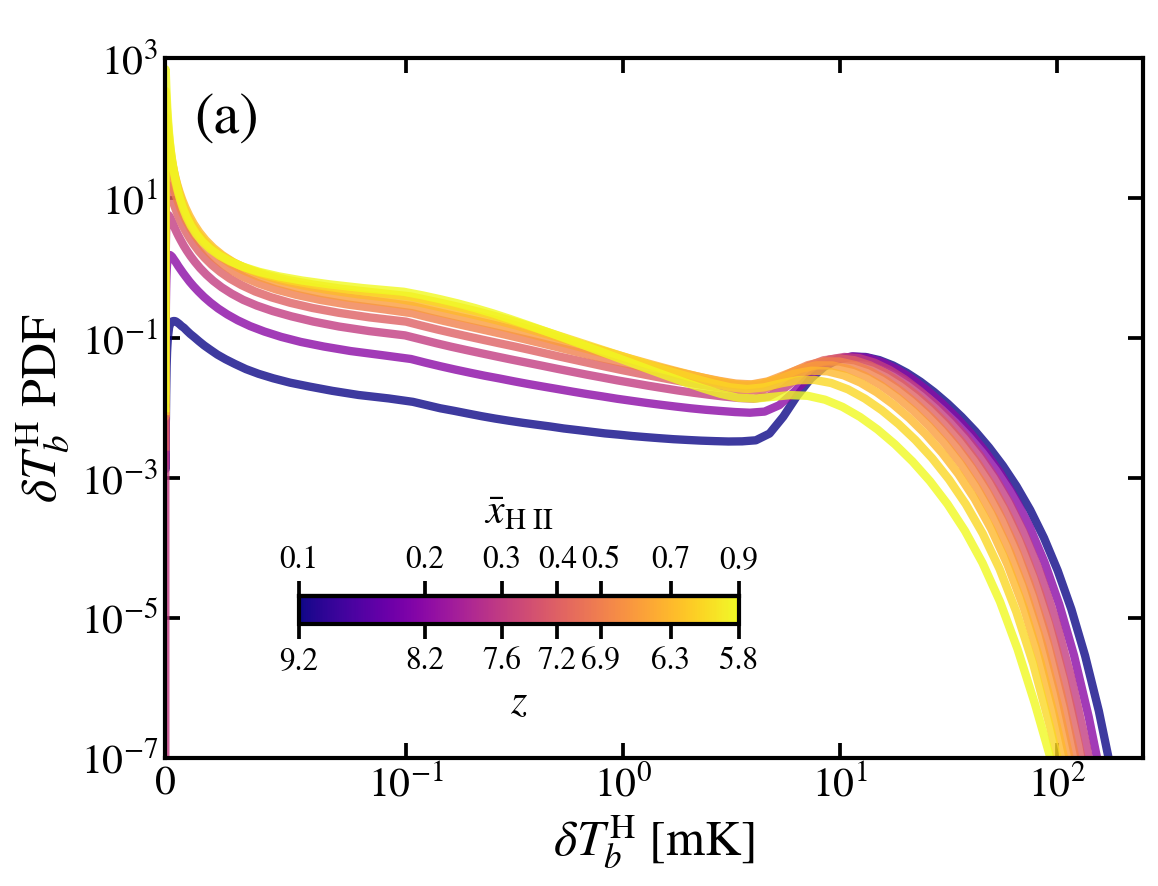
\includegraphics[width=\linewidth]{figs/vid.png}
    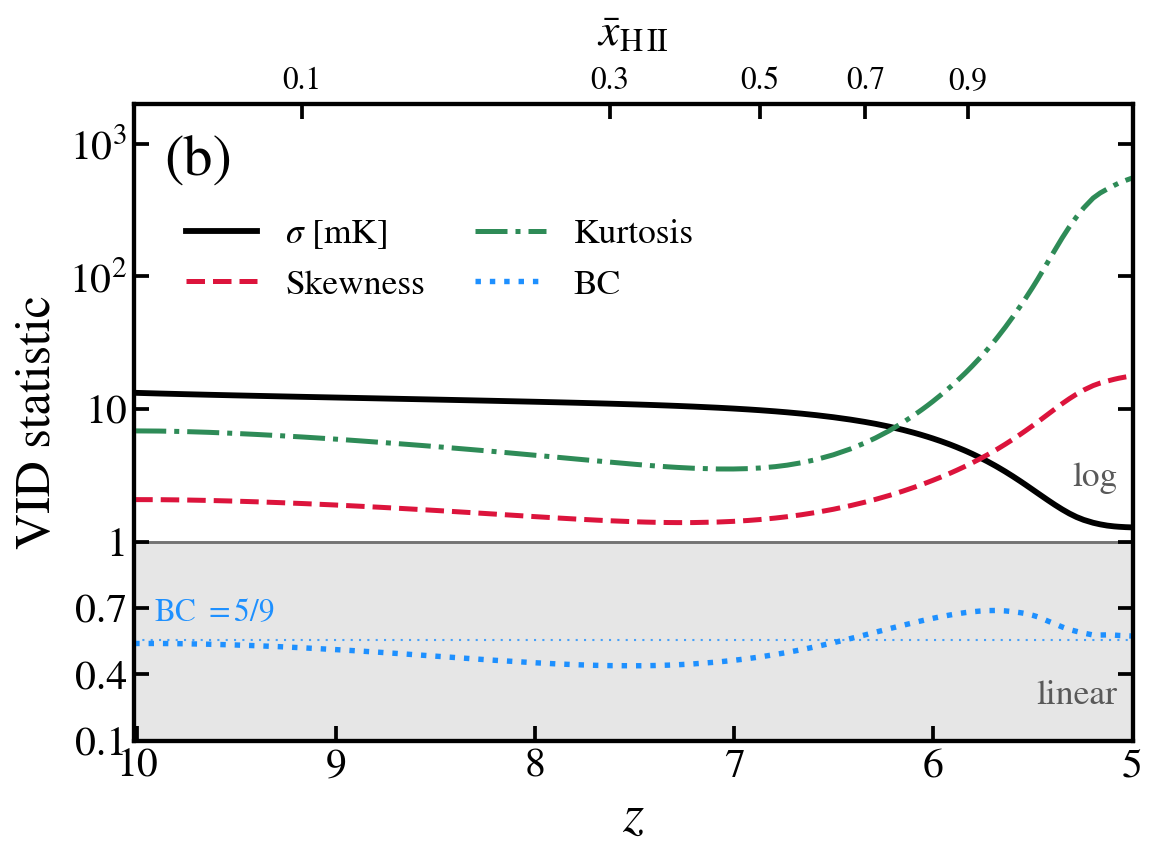
\includegraphics[width=\linewidth]{figs/sum_stat.png}
    \caption{Evolution of the VID and its higher-order summary statistics for the hydrogen 21\,cm brightness temperature. Colors indicate redshift from $z = 9.2$ (dark blue) to $z = 5.8$ (yellow), corresponding to a global ionized fraction $\bar{x}_\mathrm{H\, II}$ increasing from $0.1$ to $0.9$. Top (a): The probability density function from $z=9.2$ to $z=5.8$. Bottom (b): The redshift evolution of the standard deviation, skewness, kurtosis, and bimodality coefficient (BC) from $z=10$ to $z=5$. The blue dotted line marks $\mathrm{BC}=5/9$, the value expected for a uniform distribution. For clarity, the vertical scale in panel (b) is logarithmic above 1 and linear below 1.}
    \label{fig:vid_hydro}
\end{figure}


Figure \ref{fig:vid_hydro} (a) shows the redshift evolution of the 21\,cm brightness temperature VID, from $z = 9.2$ to the late stage of reionization regime at $z = 5.8$. Even at high redshifts (dark blue curves, $z \gtrsim 9$), the VID exhibits a markedly asymmetric, non-Gaussian shape. A broad emission peak near $\sim 10$--$20\ \mathrm{mK}$ traces the predominantly neutral IGM, while a rising low-temperature component near $\delta T_\mathrm{b}^\mathrm{H} \approx 0\ \mathrm{mK}$ reflects the early emergence of isolated \ion{H}{2} regions. The location of the emission peak tracks the mean brightness temperature of the neutral hydrogen at each epoch, providing a direct connection to the global (sky-averaged) 21\,cm signal. The pronounced asymmetry between the neutral emission peak and the low-temperature ionized component is already present at these early times, demonstrating that the VID encodes non-Gaussian information inaccessible to the power spectrum even at the onset of reionization.

\begin{figure*}[!t]
    \centering
    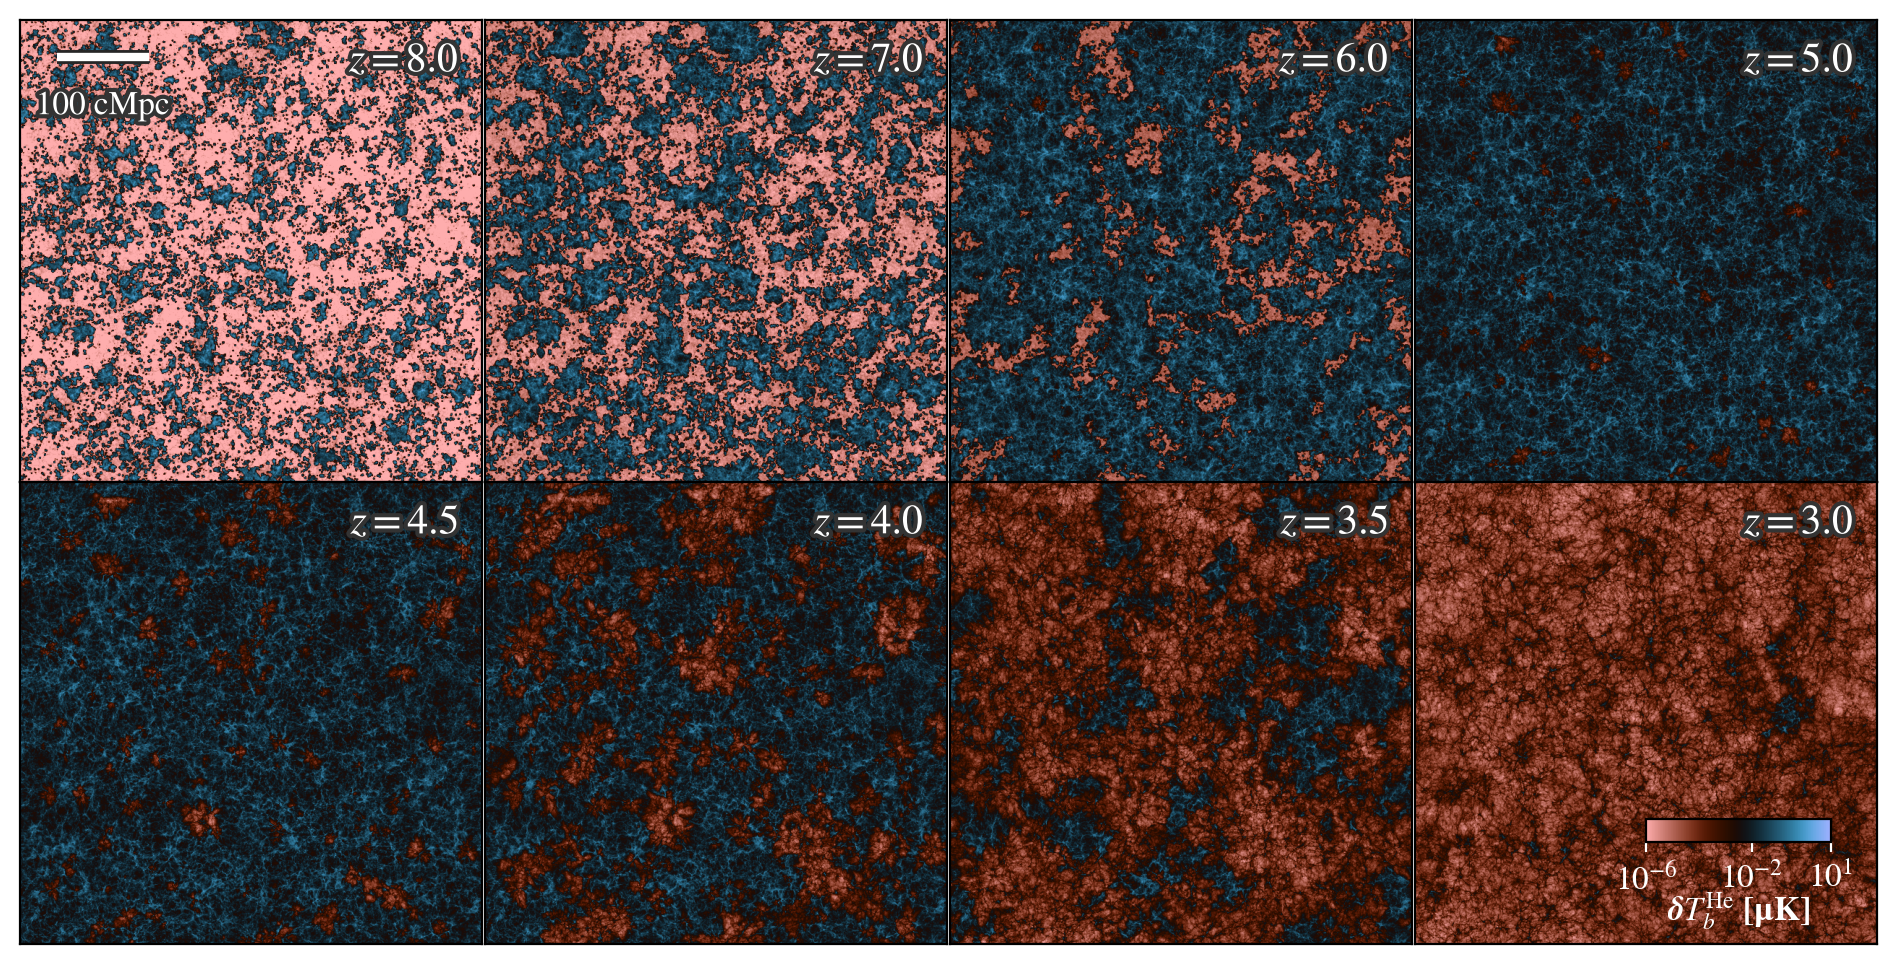
\includegraphics[width=\textwidth]{figs/tmap_helium.png}
    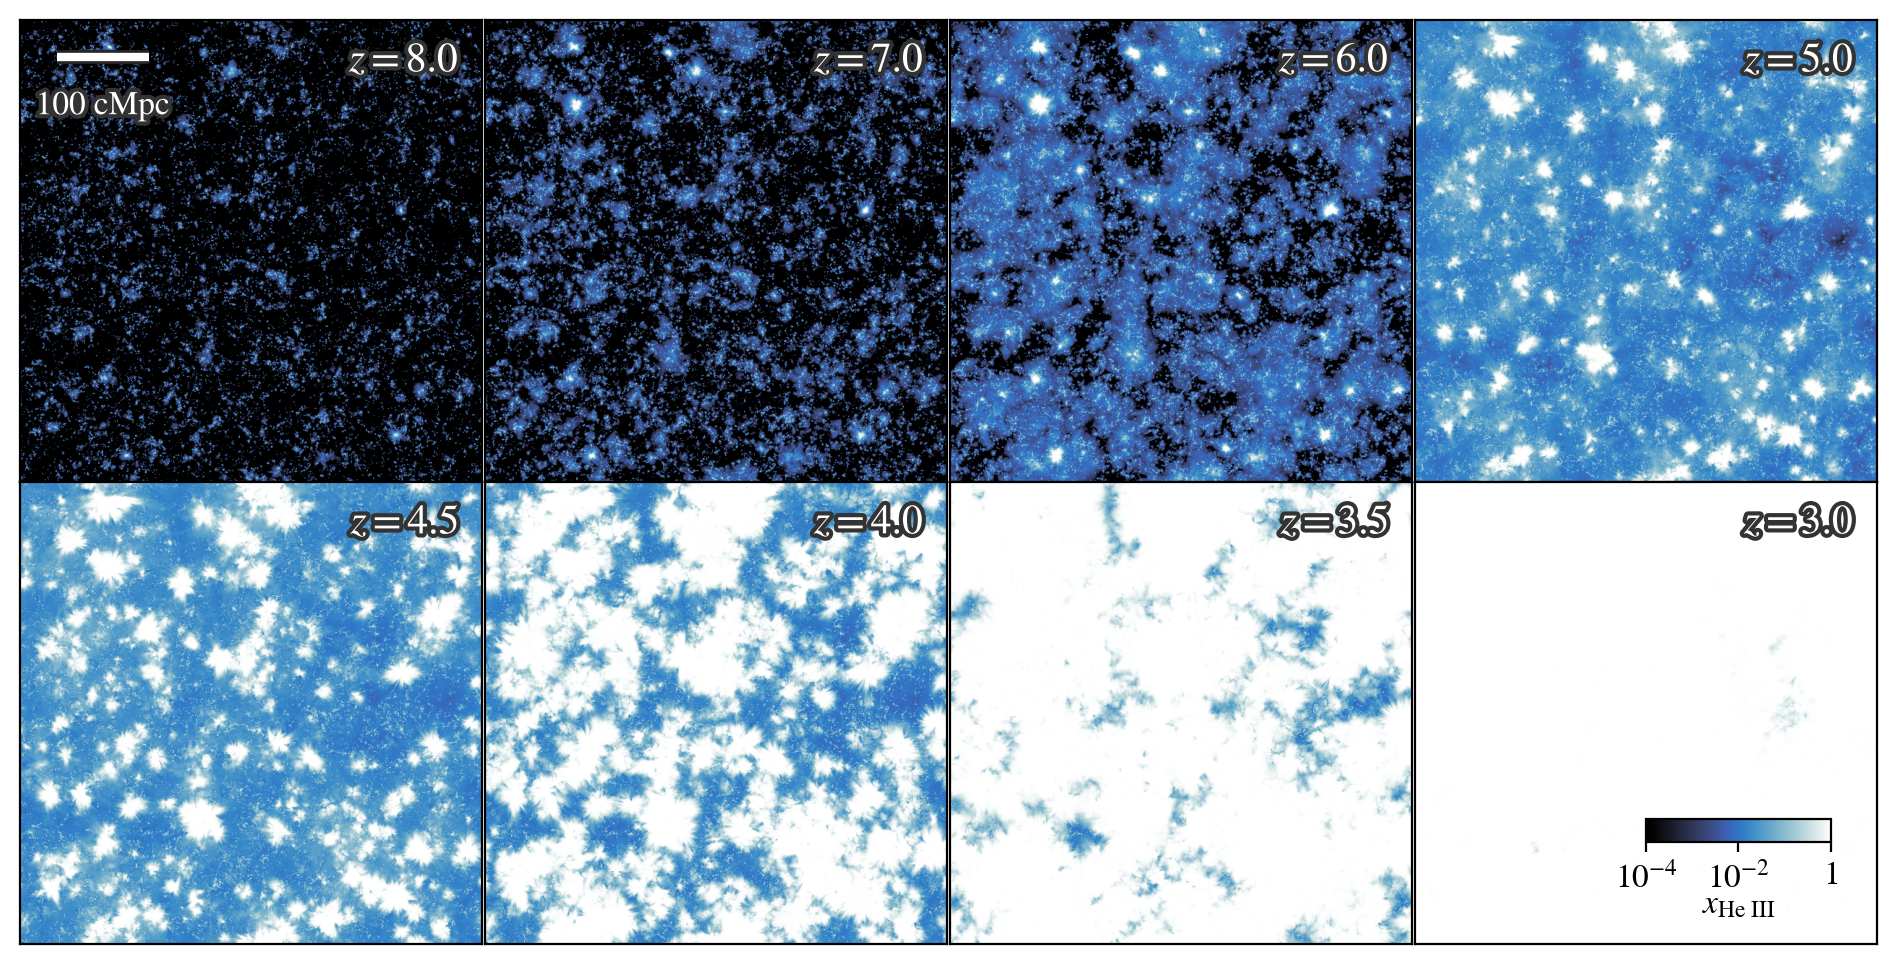
\includegraphics[width=\textwidth]{figs/f_helium.png}
    \caption{Spatial evolution of the helium 3.46\,cm brightness temperature, $\delta T^\mathrm{He}_b$ (top panels), and the fully ionized helium fraction, $f_\mathrm{HeIII}$ (bottom panels), spanning $z=8$ to $z=3$ within a $500 \, \mathrm{cMpc}$ \lumina volume.}
    \label{fig:tmap_helium}
\end{figure*}

As reionization progresses into its intermediate stages ($z \approx 7$--$8$), the VID exhibits a morphological transformation into a highly non-Gaussian distribution. The emergence of a dominant low-temperature peak (approaching $0 \ \mathrm{mK}$) traces the rapid growth and percolation of ionized regions. Simultaneously, a secondary peak persists near $10$--$20 \, \mathrm{mK}$, representing the surviving, dense neutral filaments of the cosmic web. Finally, at lower redshifts (yellow curves, $z \lesssim 6$), the Universe approaches full ionization. The high-temperature neutral peak collapses, and the distribution converges into an extreme, positively skewed spike concentrated near $0 \, \mathrm{mK}$, with only a marginal high-temperature tail indicating rare, self-shielded neutral pockets.


To quantitatively track the morphological evolution of the 21\,cm signal, we extract the standard deviation, skewness, kurtosis, and bimodality coefficient (BC) from the VID, shown in the bottom panel (b) of Figure \ref{fig:vid_hydro}. The standard deviation traces the variation of spatial fluctuations. It exhibits a monotonic decrease from its maximum at $z=10$ down to approximately 1 mK by $z=5$. This continuous decline reflects the overarching suppression of the 21\,cm emission. As expanding \ion{H}{2} regions progressively wipe out the signal, the absolute spread of the intensities inherently diminishes.


The higher-order statistics, skewness and kurtosis, provide sensitive probes of the evolving topology during the late stages of reionization. At high redshifts ($z \gtrsim 8$), both quantities remain relatively small and stable, consistent with the mildly non-Gaussian density field in a predominantly neutral IGM. Both statistics exhibit a minimum near $z \approx 7$, corresponding to a transitional stage where the growing low-temperature ionized component and the diminishing neutral emission peak make temporarily balanced contributions to the distribution, minimizing the net asymmetry. These minima occur shortly before the midpoint of reionization ($\bar{x}_\mathrm{H\,II} \approx 0.5$, $z \approx 6.9$), as the ionized and neutral volume fractions approach comparable values. At later times ($z \lesssim 7$), both skewness and kurtosis increase rapidly as reionization progresses. This evolution reflects the growing asymmetry of the signal: the distribution becomes increasingly dominated by a large fraction of near-zero brightness temperature voxels, while the remaining neutral regions contribute a diminishing but extended high-intensity tail. As a result, the kurtosis rises due to the concentration of probability near zero, and the skewness increases due to the asymmetric tail toward higher brightness temperatures.


The BC for hydrogen traces a sharp, localized phase transition driven by widespread star-forming galaxies. At early stage of the reionization ($z \ge 8$), the IGM is overwhelmingly neutral, yielding a lower BC because the gas resides almost entirely in a single neutral phase. As reionization reaches its late percolation stage ($z \approx 6.0 \to 5.7$), expanding \ion{H}{2} bubbles swallow most of the volume, creating vast, fully ionized regions that exist alongside dense, surviving neutral filaments. The BC reaches its sharp global peak of $\mathrm{BC} \approx 0.69$ at $z \approx 5.7$, marking the epoch of maximum spatial inhomogeneity immediately before reionization completes. At this critical stage, the bimodal separation between the binary states is maximized. As these final neutral islands are rapidly ionized around $z \lesssim 5.5$, the neutral state disappears, causing BC to drop steeply as the IGM shifts into a globally uniform, single-phase ionized plasma.

%%%---This part is optional for now, in case we need the observational threshold

%While the theoretical VID perfectly captures the pristine, bimodal morphology of the Epoch of Reionization, observing this signature with next-generation interferometers such as the SKA-Low introduces significant instrumental complexities. The finite angular resolution of the telescope effectively acts as a spatial low-pass filter, smoothing the underlying 21\,cm field. As demonstrated by varying the smoothing scale (R), this beam effect averages out small-scale density fluctuations and artificially suppresses the overall variance of the distribution.

%Furthermore, real-world interferometric measurements are inherently subject to thermal noise, which mathematically convolves the true physical probability distribution with a Gaussian noise profile. For deep SKA-Low observations, this thermal noise ($\sim$ 1 to 3 mK per resolution element) will inevitably broaden the sharp theoretical spikes seen in the idealized VID. If the noise amplitude or the applied smoothing scale becomes comparable to the temperature difference between the ionized bubbles and the neutral filaments, the distinct bimodality will be smeared into a single, heavily skewed curve. Consequently, forward-modeling these specific instrumental constraints using large-volume, high-resolution simulations like LUMINA is absolutely essential. It is the only way to accurately distinguish the true cosmological timeline from the blurring effects of the telescope itself.



\subsubsection{Helium VID statistics}



Figure \ref{fig:tmap_helium} shows the spatial evolution of the 3.46\,cm brightness temperature $\delta T_\mathrm{b}^\mathrm{He}$ (upper panels) and the fully ionized helium fraction $x_\mathrm{He\,III}$ (lower panels), spanning $z = 8$ to $z = 3$ within the $500\,\mathrm{cMpc}$ \lumina volume. The most striking feature is the amplitude of the helium signal ($\delta T_\mathrm{b}^\mathrm{He}$). It reaches a peak of only $\sim 0.03 \,\mu\mathrm{K}$, roughly five orders of magnitude weaker than the 21\,cm brightness temperature at comparable epochs. This difference in amplitude reflects the low abundance of the $^3$He isotope ($\sim 10^{-5}$ relative to hydrogen), which fundamentally limits the strength of the hyperfine signal and represents the primary observational challenge for detecting the 3.46\,cm line with current and future radio interferometers.


At high redshifts ($z \gtrsim 7$), the 3.46\,cm signal exhibits a highly granular, point-like morphology, with emission concentrated in small, compact regions coinciding with the densest nodes of the cosmic web. This contrasts with the broad, diffuse emission characteristic of the early 21\,cm signal, and reflects the different nature of the sources driving helium ionization. Unlike hydrogen reionization, which is driven by the collective UV radiation of stellar populations, the first ionization of helium (\ion{He}{1}\,$\rightarrow$\,\ion{He}{2}) requires photons above 24.6\,eV. While massive stars can produce such photons, they do so less efficiently than for hydrogen ionization, concentrating the signal around the densest star-forming halos rather than spreading it uniformly across the IGM. During this early phase, the fully ionized helium fraction $x_\mathrm{He\,III}$ remains negligible across most of the volume (lower panels, $z \gtrsim 7$), as the hard extreme-UV photons required for the second ionization stage (\ion{He}{2} $\rightarrow$ \ion{He}{3}) have not yet become sufficiently abundant to drive large-scale double ionization.

\begin{figure}[!t]
    \centering
    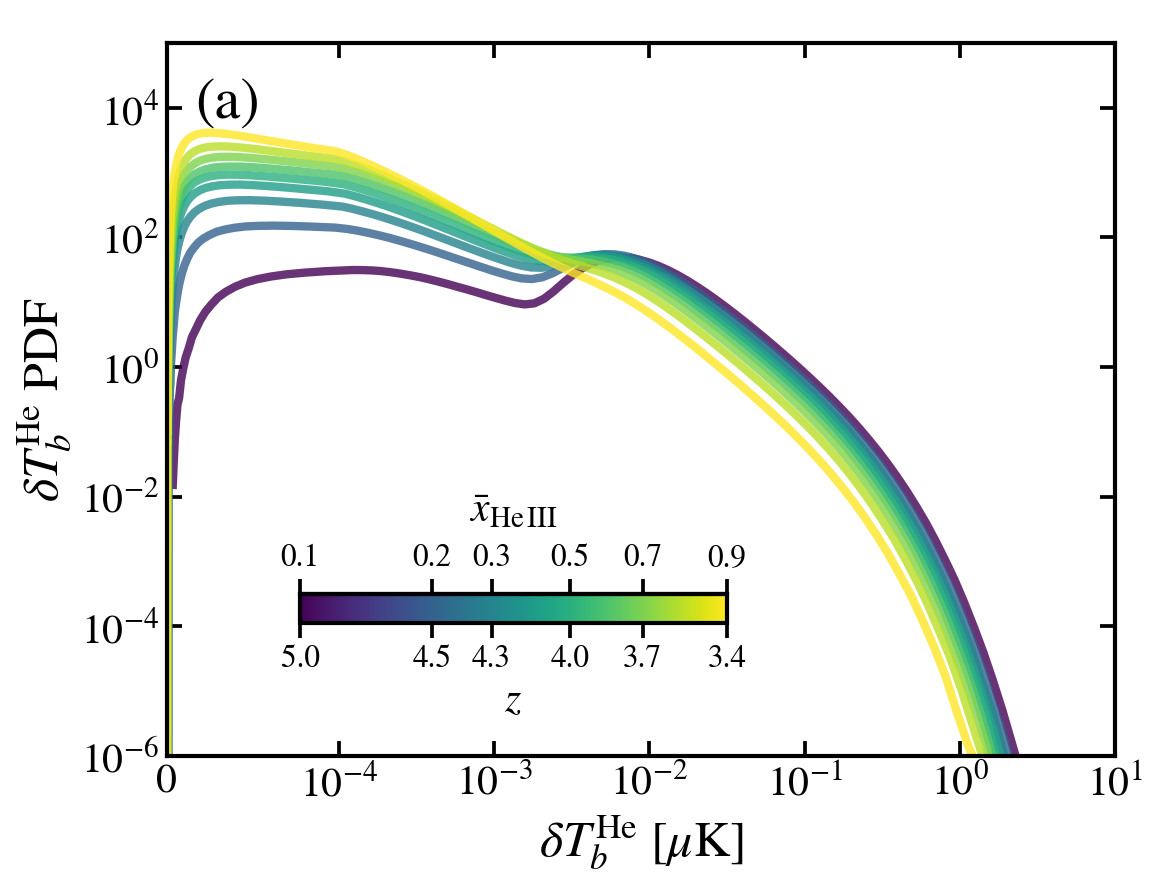
\includegraphics[width=\linewidth]{figs/vid_He.png}
    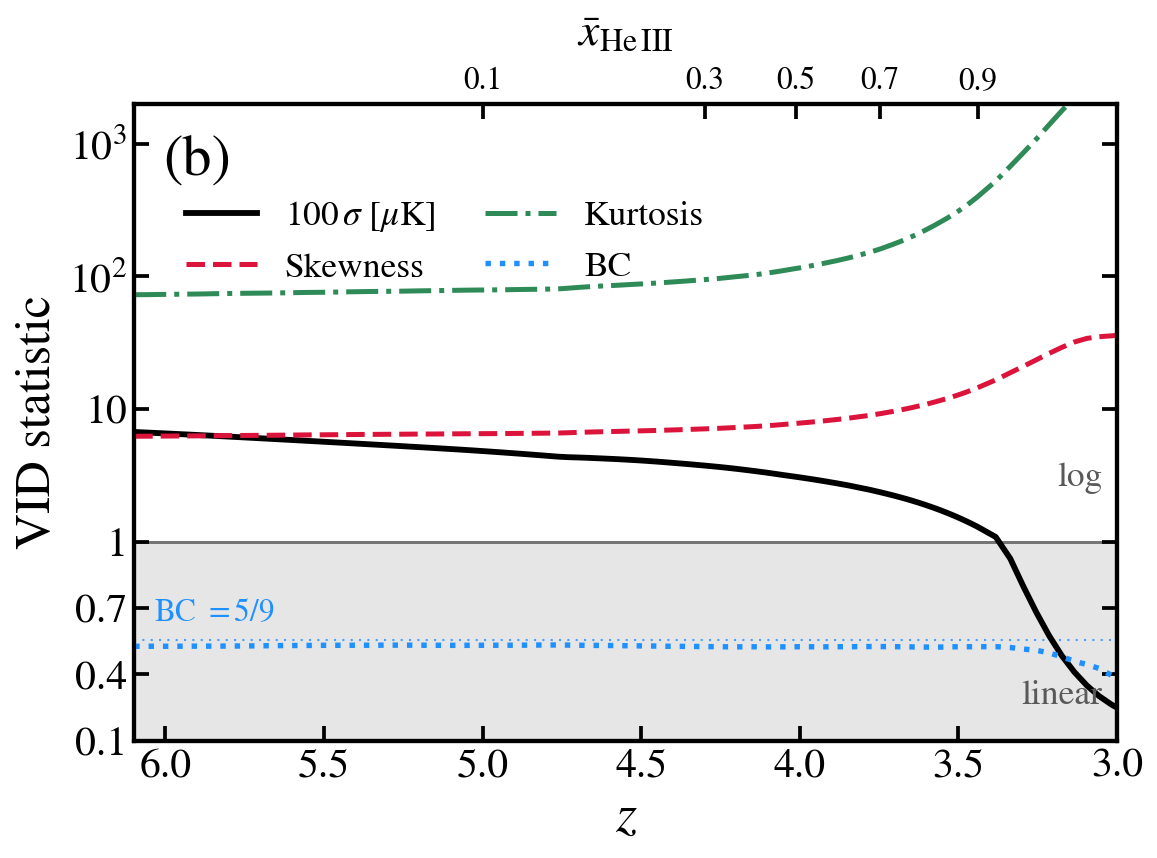
\includegraphics[width=\linewidth]{figs/sum_stat_He.png}
    \caption{Evolution of the VID and its higher-order summary statistics for the helium 3.46\,cm brightness temperature. Colors indicate redshift from $z = 5$ (dark purple) to $z = 3.4$ (yellow), corresponding to a global ionized fraction $\bar{x}_\mathrm{He\, III}$ increasing from $0.1$ to $0.9$. Top (a): The probability density function from $z=5$ to $z=3.4$ . Bottom (b): The redshift evolution of the standard deviation, skewness, kurtosis, and BC from $z=6$ to $z=3$.}
    \label{fig:vid_helium}
\end{figure}


Around $z \approx 5$--$6$, the 3.46\,cm signal reaches its peak amplitude and undergoes a morphological transition from the compact, source-centered emission of earlier epochs to a more extended, filamentary structure. This transition reflects the build-up of a widespread \ion{He}{2} background as stellar populations and early AGN collectively ionize the bulk of the neutral helium, producing a broadly distributed singly ionized medium. Crucially, however, the resulting emission does not simply trace the matter density field: unlike the hydrogen case, the IGM is generally not thermally saturated for the 3.46\,cm transition. $T_S^{\rm He} \approx T_K$ is approached only near AGN and strongly star-forming regions, where \ion{He}{2} Ly$\alpha$ coupling and electron collisions are efficient, while across most of the volume the signal remains sensitive to the spatially varying spin temperature. The 3.46\,cm brightness temperature therefore retains its full dependence, $\delta T_b^{\rm He} \propto x_{\rm HeII}\,(1+\delta_b)\,(1 - T_\gamma/T_S^{\rm He})$, with the emission strongest in dense, source-illuminated filaments and halos where the \ion{He}{2} fraction, the baryon overdensity, and the coupling are all elevated. The resulting maps at $z \approx 5$ thus trace not simply the large-scale density field but the coupled structure of helium ionization and radiative heating at the peak of helium reionization, with the filamentary pattern reflecting the same cosmic web topology that drives the non-Gaussian bispectrum signatures discussed in Section \ref{sec:bispectrum}.


At $z \lesssim 5$, quasar activity intensifies, driving the second ionization stage (\ion{He}{2} $\rightarrow$ \ion{He}{3}) and progressively depleting the \ion{He}{2} reservoir that produces the 3.46\,cm signal. The growing \ion{He}{3} regions are visible in the upper panels as expanding zero-signal voids, where helium has been fully doubly ionized and can no longer produce a spin-flip transition. The lower panels show the corresponding growth of $x_\mathrm{He\,III}$, concentrated around the most overdense, quasar-rich environments, which are doubly ionized first in an inside-out fashion. Consequently, the residual \ion{He}{2} signal is progressively displaced toward underdense filaments and voids, where the hard ionizing radiation field has not yet penetrated sufficiently to complete the second ionization. As reionization progresses through $z \approx 3.5$--$4$, the \ion{He}{3} regions expand and percolate, confining the remaining \ion{He}{2} emission to an increasingly narrow network of low-density structures. By $z \approx 3$, helium reionization is largely complete, and the 3.46\,cm signal has faded across virtually the entire volume, with only faint traces persisting in the most underdense regions where the local ionizing radiation field remains weakest.

% put the VID helium figure here




Figure \ref{fig:vid_helium} (a) shows the redshift evolution of the VID of the 3.46\,cm brightness temperature, spanning from $z = 5$ ($\bar{x}_\mathrm{He\,III} = 0.1$, dark purple) to $z = 3.4$ ($\bar{x}_\mathrm{He\,III} = 0.9$, yellow). The overall evolutionary behavior closely mirrors that of the hydrogen VID, differing primarily in amplitude, redshift range, and temperature scale. At $z = 5$, the distribution is characterized by a dominant peak near $\approx 0.01\ \mu\mathrm{K}$, which tracks the mean global 3.46\,cm brightness temperature at that epoch, alongside a broad high-temperature tail extending to $\gtrsim 1\ \mu\mathrm{K}$ that reflects the range of local \ion{He}{2} fractions and baryon overdensities across the simulation volume. As emphasized above, the IGM is generally not thermally saturated for the 3.46\,cm transition, so the brightness temperature retains its full dependence on $x_\mathrm{He\,II}(1+\delta_b)(1-T_\gamma/T_S^\mathrm{He})$. The distribution, therefore, traces the joint variation of the local ionization state, matter density, and spin-temperature coupling across the volume.


As reionization proceeds toward lower redshifts ($z \lesssim 4.5$, transitioning from blue to yellow curves), quasar-driven ionization increasingly dominates the IGM. The impact of the expanding \ion{He}{3} regions is clearly reflected in the PDF: the high-intensity emission tail steadily decreases in probability density, while a growing fraction of voxels accumulates in a pronounced spike near $0$ $\mu$K. Because fully ionized \ion{He}{3} no longer produces a hyperfine signal, this zero-signal component provides a direct proxy for the volumetric growth of quasar-driven ionized regions. By $z \approx 3.4$, the signal is suppressed across most of the volume, marking the near completion of helium reionization.


%As helium reionization progresses toward lower redshifts ($z \lesssim 4.5$), quasar activity drives the \ion{He}{2} $\rightarrow$ \ion{He}{3} transition, progressively depleting the \ion{He}{2} reservoir. This depletion is directly reflected in the VID: the dominant peak shifts toward lower temperatures and the high-temperature tail steadily shrinks as the overall \ion{He}{2} fraction declines, reducing the brightness temperature across the volume. Simultaneously, the low-temperature component near $\delta T_\mathrm{b}^\mathrm{He} \approx 0$ grows as an increasing fraction of voxels become fully doubly ionized into \ion{He}{3}, which produces no 3.46\,cm signal. This zero-signal component therefore serves as a proxy for the growth of \ion{He}{3} regions, analogous to the ionized zero-signal component in the hydrogen VID. By $z \approx 3.4$, the peak has collapsed toward zero and the signal is suppressed across most of the volume, marking the near completion of helium reionization.



To further quantify this evolution, we examine the higher-order summary statistics of the 3.46\,cm VID from $z = 6$ to $z = 3$, shown in Figure \ref{fig:vid_helium} (b). The standard deviation remains high and relatively stable from $z = 6$ to $z \approx 3.5$, reflecting the widespread \ion{He}{2} emission that sustains large spatial fluctuations during the active phase of helium reionization. Beyond this point, the standard deviation drops sharply as quasar activity rapidly depletes the \ion{He}{2} reservoir, suppressing spatial fluctuations across the volume as the IGM transitions to a predominantly \ion{He}{3} state.


The skewness and kurtosis rise toward the end of helium reionization, as in hydrogen, but unlike hydrogen they show no minimum. Throughout the \ion{He}{2}-dominated era both rise slowly but monotonically (skewness $\approx 6.3 \to 7.9$ and kurtosis $\approx 73 \to 114$ from $z = 6$ to $4$), and both are already far larger than their hydrogen counterparts at comparable ionized fractions, because the helium signal is concentrated in a heavy tail of strongly coupled, overdense voxels. As the Universe approaches full helium ionization ($z \lesssim 4$), both skewness and kurtosis rise rapidly, with the kurtosis reaching exceptionally large values exceeding $10^3$ by $z \approx 3.2$. This behavior reflects the transition to a regime where the most overdense, quasar-rich environments have already been fully doubly ionized, while the residual \ion{He}{2} emission becomes increasingly confined to underdense filamentary structures at the periphery of the \ion{He}{3} regions. Consequently, not only does the zero-signal component grow as more volume becomes fully ionized, but the high-temperature tail also shrinks as the brightest, densest \ion{He}{2} structures are progressively consumed, leaving only fainter filamentary emission. The resulting distribution is dominated by a large zero-signal component punctuated by rare, faint filamentary outliers. This produces large positive skewness and extreme kurtosis, reflecting the concentrated and spatially asymmetric nature of the final stages of helium reionization.


For helium double-ionization, the BC exhibits an extended plateau followed by a sudden collapse, reflecting the distinct nature of quasar-driven reionization. Throughout $z \approx 6.0 \to 3.5$, BC remains consistently elevated ($\mathrm{BC} \sim 0.51$--$0.55$) because rare, luminous quasars slowly carve out isolated \ion{He}{3} proximity zones within a predominantly \ion{He}{2} IGM. At this late percolation stage ($z \lesssim 3.5$), giant, interconnected \ion{He}{3} regions co-exist with the final surviving \ion{He}{2} patches, maximizing the statistical contrast between the binary ionization states. As these remaining \ion{He}{2} islands are swept up toward $z \approx 3.0$, the \ion{He}{2} phase vanishes entirely, causing BC to crash steeply below $0.4$ as the IGM completes its transition into a globally uniform, single-phase \ion{He}{3} plasma.


%We omit the mean brightness temperature, as it closely follows the global 3.46\,cm signal discussed earlier. The variance (top-right panel) exhibits a steady monotonic decline from $z=6$ to $z=3$. This continuous decrease reflects the progressive suppression of spatial fluctuations as quasar-driven \ion{He}{3} regions expand, percolate, and gradually remove the emitting \ion{He}{2} medium.



\subsection{Power spectrum}

The power spectrum serves as the primary statistical tool for quantifying the spatial structure of the IGM, decomposing the brightness temperature and ionization fields into Fourier modes to provide a scale-dependent description of fluctuations across different physical scales. It provides a robust and observationally accessible measure of the characteristic scales and amplitude of reionization-driven fluctuations. It cannot capture the full non-Gaussian morphology of ionized  bubbles, a limitation addressed by the higher-order statistics presented in  Section \ref{sec:bispectrum}, but it serves as a natural complement to the  VID and bispectrum analyses presented in this work.


The 21\,cm and 3.46\,cm brightness temperature signals each reflect the combined contributions of the matter density field, the ionized fraction, and the thermal evolution of the IGM, making it difficult to isolate the individual role of each component from the observable signal alone. To disentangle these contributions, we analyze the power spectra of both the observable brightness temperatures and their corresponding ionization fraction fields, which serve as clean indicators of the ionization history and topology, free from the additional modulation by density and thermal structure. By comparing the two directly, we can isolate the contribution of the ionization topology and investigate how baryon overdensity and thermal evolution modulate the observable signal. Furthermore, the characteristic scale of ionized regions leaves distinct imprints on both sets of power spectra: the dominant bubble size is encoded in the peak of the ionization fraction power spectrum, while the shoulder of the brightness temperature power spectrum provides a complementary observable-based probe of the same physical scale \citep[][]{Furlanetto2006}. These signatures are discussed further in the context of the bubble size analysis in Section \ref{sec:bubble}.


To characterize reionization across both hydrogen and helium epochs, we analyze the dimensionless power spectra of the ionized hydrogen fraction $\Delta^2_{x_\mathrm{H\,II}}(k)$, the 21\,cm brightness temperature $\Delta^2_\mathrm{H}(k)$, the doubly ionized helium fraction $\Delta^2_{x_\mathrm{He\,III}}(k)$, and the 3.46\,cm brightness temperature $\Delta^2_\mathrm{He}(k)$. For the hydrogen fields, we additionally compare our predictions against the \textsc{thesan-1} simulation to contextualize the impact of the larger \lumina volume on the recovered power spectrum, and against current observational upper limits and future projected sensitivities from radio interferometers to assess the detectability of the predicted signal. %The helium power spectra are presented without an external simulation comparison, as large-volume predictions of the 3.46\,cm signal remain scarce in the literature, making \lumina one of the few simulations capable of providing robust statistical predictions at these scales.



\subsubsection{Hydrogen power spectrum}

\begin{figure*}[!t]
    \centering
    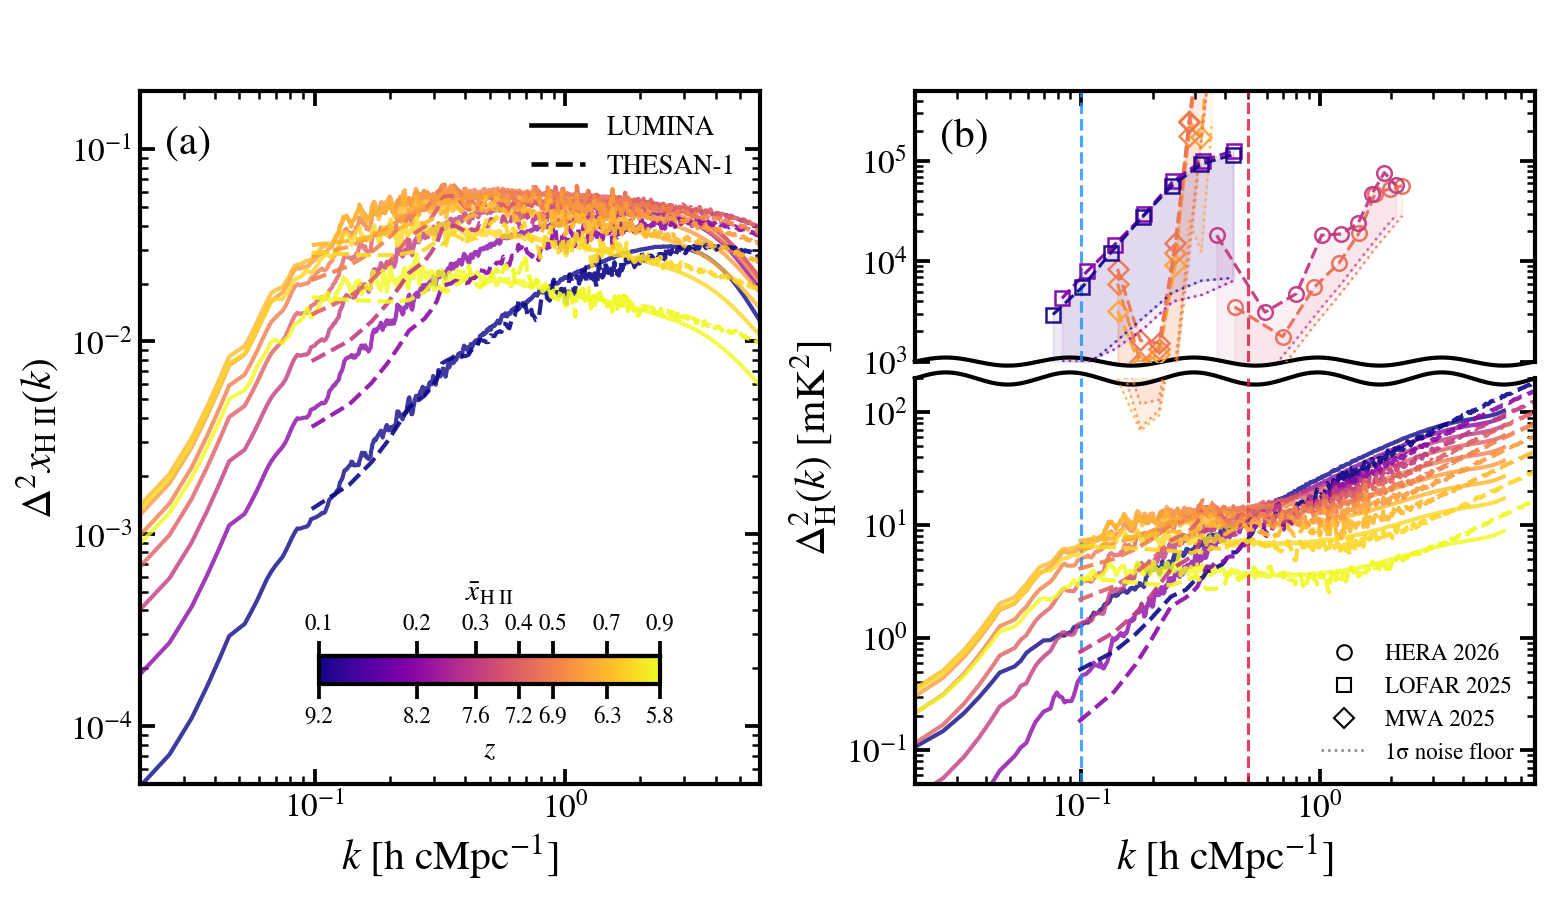
\includegraphics[width=\linewidth]{figs/ps_hydro.png}
    \par\medskip
    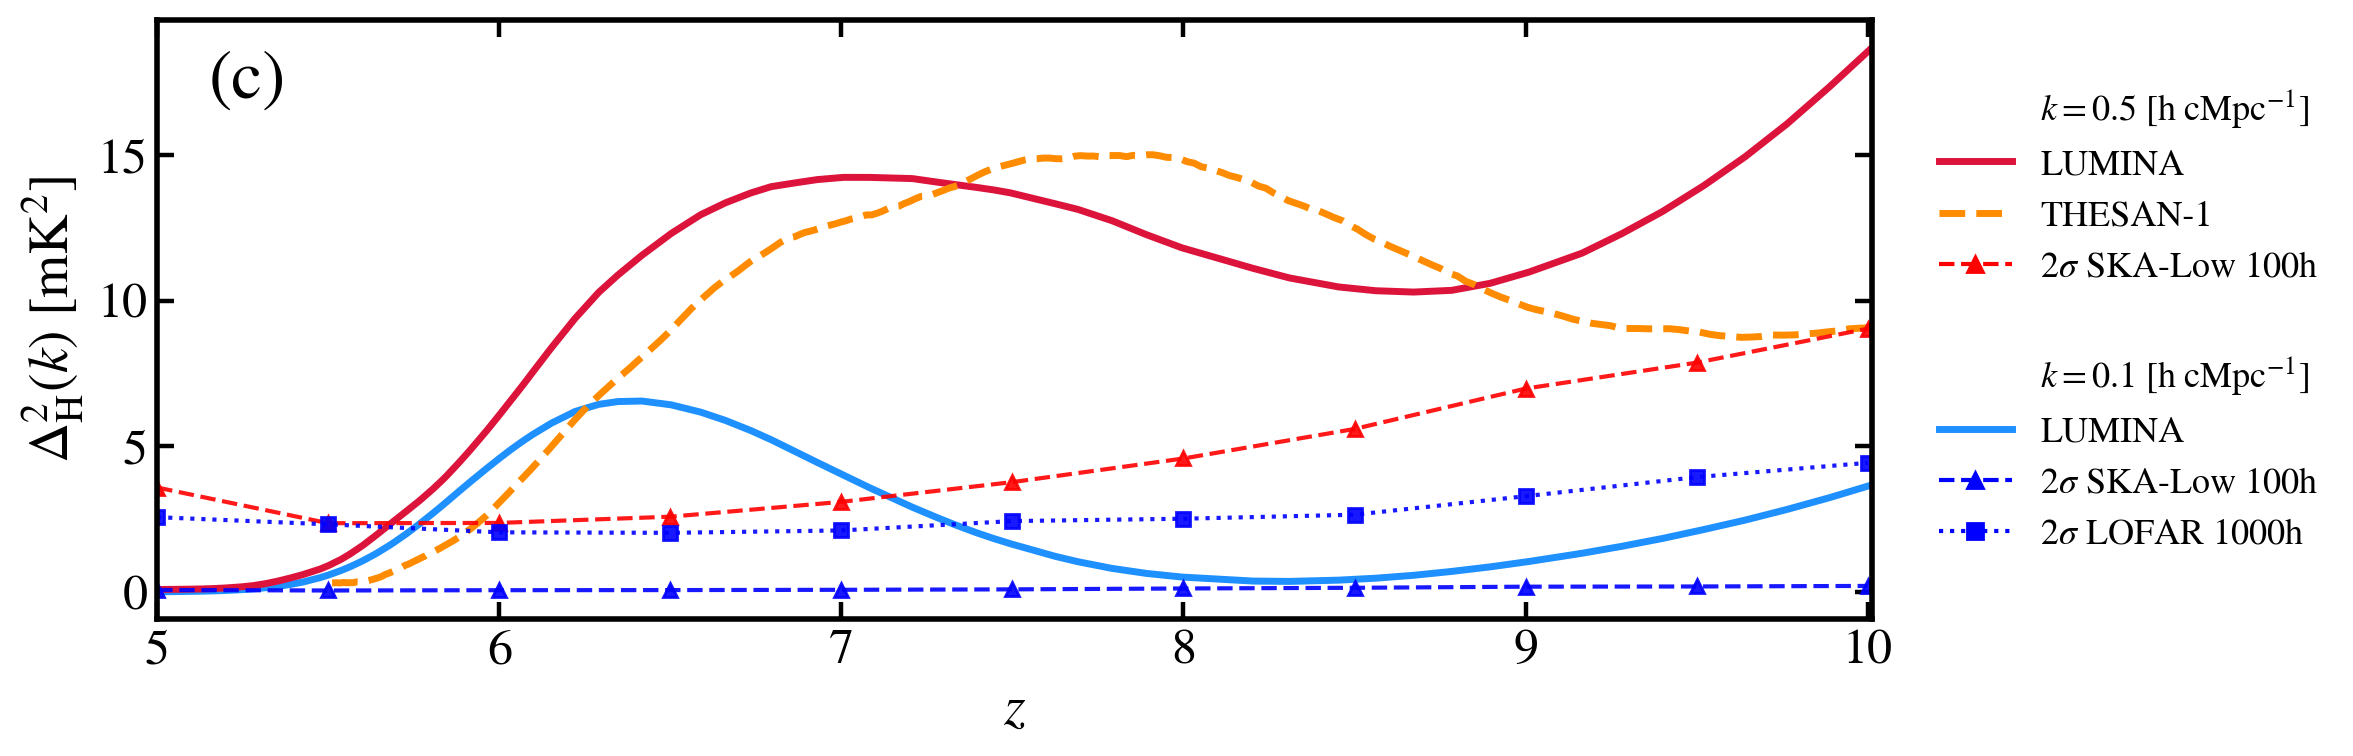
\includegraphics[width=\linewidth]{figs/PS_H_z.png}
    \caption{Redshift evolution of the dimensionless power spectra for the ionized hydrogen fraction $\Delta^2_{x_\mathrm{H\,II}}(k)$ (panel a) and the 21\,cm brightness temperature $\Delta^2_\mathrm{H}(k)$ (panel b), with solid and dashed curves representing \lumina and \textsc{thesan-1} respectively. Colors indicate redshift from $z = 9.2$ (dark blue) to $z = 5.8$ (yellow), corresponding to a global ionized fraction $\bar{x}_\mathrm{H\, II}$ increasing from $0.1$ to $0.9$. Panel (b) also shows current observational upper limits and 1$\sigma$ noise floor from HERA \citep[][]{HERA2026}, LOFAR \citep[][]{Mertens2025}, and MWA \citep[][]{Nunhokee2025}, with vertical dashed lines marking $k = 0.1$ (blue) and $0.5\,h\,\mathrm{cMpc}^{-1}$ (red). Panel (c) shows the redshift evolution of $\Delta^2_\mathrm{H}(k)$ at $k = 0.1$ and $0.5\,h\,\mathrm{cMpc}^{-1}$ from $z = 10$ to $z = 5$ for \lumina (solid curves), alongside the \textsc{thesan-1} result at $k = 0.5\,h\,\mathrm{cMpc}^{-1}$ (orange dashed curve). The red and blue dashed curves show the simulated $2\sigma$ thermal noise sensitivity of SKA-Low \citep[][]{Barry2022} (triangles) at $k = 0.5$ and $0.1\,h\,\mathrm{cMpc}^{-1}$, respectively, assuming 100 hours of integration, and the blue dotted curve shows the corresponding LOFAR-HBA \citep[][]{vanHaarlem2013} sensitivity (squares) at $k = 0.1\,h\,\mathrm{cMpc}^{-1}$ for 1000 hours.}
    \label{fig:ps_hydro}
\end{figure*}
% \citet{Munshi2025}
% \citet{Trott2025}
% , with \textcolor{red}{(WILL BE ADDED)} indicating the current observational threshold

Figure \ref{fig:ps_hydro} presents the redshift evolution of the dimensionless power spectra for the ionized hydrogen fraction $\Delta^2_{x_\mathrm{H\,II}}(k)$ (panel a) and the 21\,cm brightness temperature $\Delta^2_\mathrm{H}(k)$ (panel b), with solid and dashed curves representing \lumina and \textsc{thesan-1} \citep{Kannan2022, Kannan2022b} respectively, color-coded by redshift from $z = 9.2$ (dark blue) to $z = 5.8$ (yellow) corresponding to $\bar{x}_\mathrm{H\,II}$ increasing from $0.1$ to $0.9$. Panel (c) shows the redshift evolution of $\Delta^2_\mathrm{H}(k)$ at two representative wavenumbers $k = 0.1$ and $0.5\,h\,\mathrm{cMpc}^{-1}$, indicated by the vertical dashed lines in panel (b).



Panel (a) traces the evolution of the ionization topology through the power spectrum of the ionized fraction field. At early times ($z \sim 9$--$10$), the power is weak and peaks at relatively high wavenumbers ($k \gtrsim 1\,h\,\mathrm{cMpc}^{-1}$), indicating that ionized regions are initially small and spatially isolated around the first galaxies. As reionization progresses, the amplitude of $\Delta^2_{x_\mathrm{H\,II}}$ increases while the peak systematically migrates toward lower $k$, reflecting the expansion and merger of \ion{H}{2} regions into larger coherent structures and providing a direct statistical tracer of the characteristic ionized bubble scale \citep[e.g.,][]{Lidz2008, Furlanetto2006, Mesinger2019}. In Section \ref{sec:bubble}, we examine this redshift evolution in detail, comparing the bubble scales inferred from power spectrum peaks against real-space bubble size distributions for \ion{H}{2}. Near the completion of reionization ($z \lesssim 6$), the power declines across all scales as the ionization field approaches a fully ionized state, reducing the spatial contrast that sources the fluctuation power.


Comparing \lumina with \textsc{thesan-1} reveals a scale-dependent difference set by the complementary strengths of the two simulations. Here we match the two simulations by ionized fraction rather than redshift, isolating morphological effects from differences in reionization timing. At low $k$ ($\lesssim 0.3\,h\,\mathrm{cMpc}^{-1}$), \lumina exhibits slightly higher power at fixed ionized fraction. Its larger volume captures the more extended ionized structures and suppresses the finite-box truncation of long-wavelength modes that affects smaller boxes such as \textsc{thesan-1}. At intermediate $k$ ($\sim 0.3$--$1\,h\,\mathrm{cMpc}^{-1}$) the two spectra agree closely, indicating that the bulk ionization morphology is consistent between the models. At the highest $k$ ($\gtrsim 3\,h\,\mathrm{cMpc}^{-1}$), however, \lumina falls below \textsc{thesan-1}. With a coarser grid resolution, \lumina progressively under-resolves the small-scale ionized structure and the dense absorbers that regulate it, suppressing power as the grid scale is approached. This crossover reflects the fact that  \lumina is optimized for the large-scale modes ($k \lesssim 0.1\,h\,\mathrm{cMpc}^{-1}$) targeted by SKA and HERA, while \textsc{thesan-1} retains an advantage on the smallest scales.


Panel (b) shows how this evolving ionization topology is imprinted on the observable 21\,cm signal. At high redshift ($z \gtrsim 9$), before significant bubble growth, the 21\,cm power spectrum is primarily driven by underlying matter density fluctuations and rises monotonically toward smaller scales. As reionization approaches its midpoint ($z \approx 7$--$8$), the emergence of large ionized regions boosts the large-scale power and produces a characteristic flattening, or ``shoulder,'' around $k \sim 0.1\,h\,\mathrm{cMpc}^{-1}$, reflecting the increasing spatial contrast between expanding zero-signal ionized regions and the remaining neutral hydrogen. At later stages ($z \lesssim 6$), the power decreases as the neutral hydrogen reservoir is progressively depleted.


We compare our predicted 21\,cm power spectra against the deepest currently available observational upper limits spanning the redshift range of our simulation (upper portion of Figure \ref{fig:ps_hydro} (b)). These include the LOFAR North Celestial Pole limits of \citet{Mertens2025} at $z=8.3$ and $9.1$, derived from approximately 140 hours of observations across the ten highest-quality nights; the MWA EoR0-field limits of \citet{Nunhokee2025} at $z=6.5$--$7$ based on 268 hours of integration; and the HERA Phase II limits \citep[][at $z=7.05$ and $7.63$]{HERA2026}. Together, these experiments probe complementary Fourier scales, with LOFAR constraining the largest modes ($k \approx 0.07$--$0.4\,h\,\mathrm{cMpc}^{-1}$), MWA the intermediate scales ($k \approx 0.14$--$0.35\,h\,\mathrm{cMpc}^{-1}$), and HERA extending to smaller scales ($k \approx 0.4$--$2\,h\,\mathrm{cMpc}^{-1}$). For each measurement, we overlay both the reported $2\sigma$ upper limit and the associated $1\sigma$ noise floor (dotted curves and shaded bands), the latter setting the threshold a signal must exceed to be recoverable above thermal and residual systematic noise.


These thresholds are not directly comparable across experiments: the noise budget combines thermal noise and sample variance for the MWA \citep{Nunhokee2025}, is dominated by thermal noise for HERA \citep{HERA2026}, and is set by residual foreground power after Gaussian process regression for LOFAR \citep{Mertens2025}. They should therefore be read as survey-specific sensitivity floors rather than a single uniform curve.


The \lumina and \textsc{thesan-1} predictions for $\Delta^2_\mathrm{H}(k)$ agree closely across most of the probed range, diverging only at the largest and smallest scales, where differences in box size and resolution become apparent. At all scales probed by LOFAR, HERA, and MWA, current observational limits remain well above both predictions. Closing this gap will rely on deeper integrations and next-generation observations with interferometers such as HERA, LOFAR, and the upcoming SKA-Low.


%At the largest scales probed by LOFAR and the smallest probed by HERA, the present limits remain roughly two to three orders of magnitude above both predictions. Across most of the observable $k$-range, the 21\,cm signal from our simulations therefore remains well below current detectability. Deepening integrations, in particular the forthcoming full HERA Phase II dataset, will be required to close this gap.


Panel (c) tracks the temporal evolution of $\Delta^2_\mathrm{H}(k)$ at the two fixed wavenumbers marked in panel (b), corresponding to physical scales of $r \sim 2.5/k \approx 25\,h^{-1}\,\mathrm{cMpc}$ ($k = 0.1\,h\,\mathrm{cMpc}^{-1}$) and $r \sim 5\,h^{-1}\,\mathrm{cMpc}$ ($k = 0.5\,h\,\mathrm{cMpc}^{-1}$). At high redshift ($z \gtrsim 9$), both modes are dominated by matter density fluctuations. Around $z \sim 8.5$, both exhibit a temporary dip, marking the transition from a density-dominated to an ionization-dominated signal as the first galaxies ionize their local overdense environments, generating an anti-correlation between matter density and the neutral hydrogen fraction that partially suppresses the power. Following this transition, both modes rise as \ion{H}{2} regions expand, but on distinct timescales: the small-scale mode ($k = 0.5\,h\,\mathrm{cMpc}^{-1}$) peaks earlier at $z \approx 7$, while the large-scale mode ($k = 0.1\,h\,\mathrm{cMpc}^{-1}$) peaks later at $z \approx 6.3$, because the 21\,cm fluctuations are maximized when the characteristic ionized bubble size matches the physical scale probed by each wavenumber ($R_\mathrm{ion} \sim 2.5/k_\mathrm{peak}$). This scale-dependent peak timing is consistent with an inside-out reionization scenario, in which small isolated bubbles form first before merging into the large coherent structures that drive large-scale power at later times. As reionization nears completion ($z \lesssim 6$), the neutral hydrogen reservoir is progressively depleted and the power at both scales declines rapidly.


\begin{figure*}[!t]
    \centering
    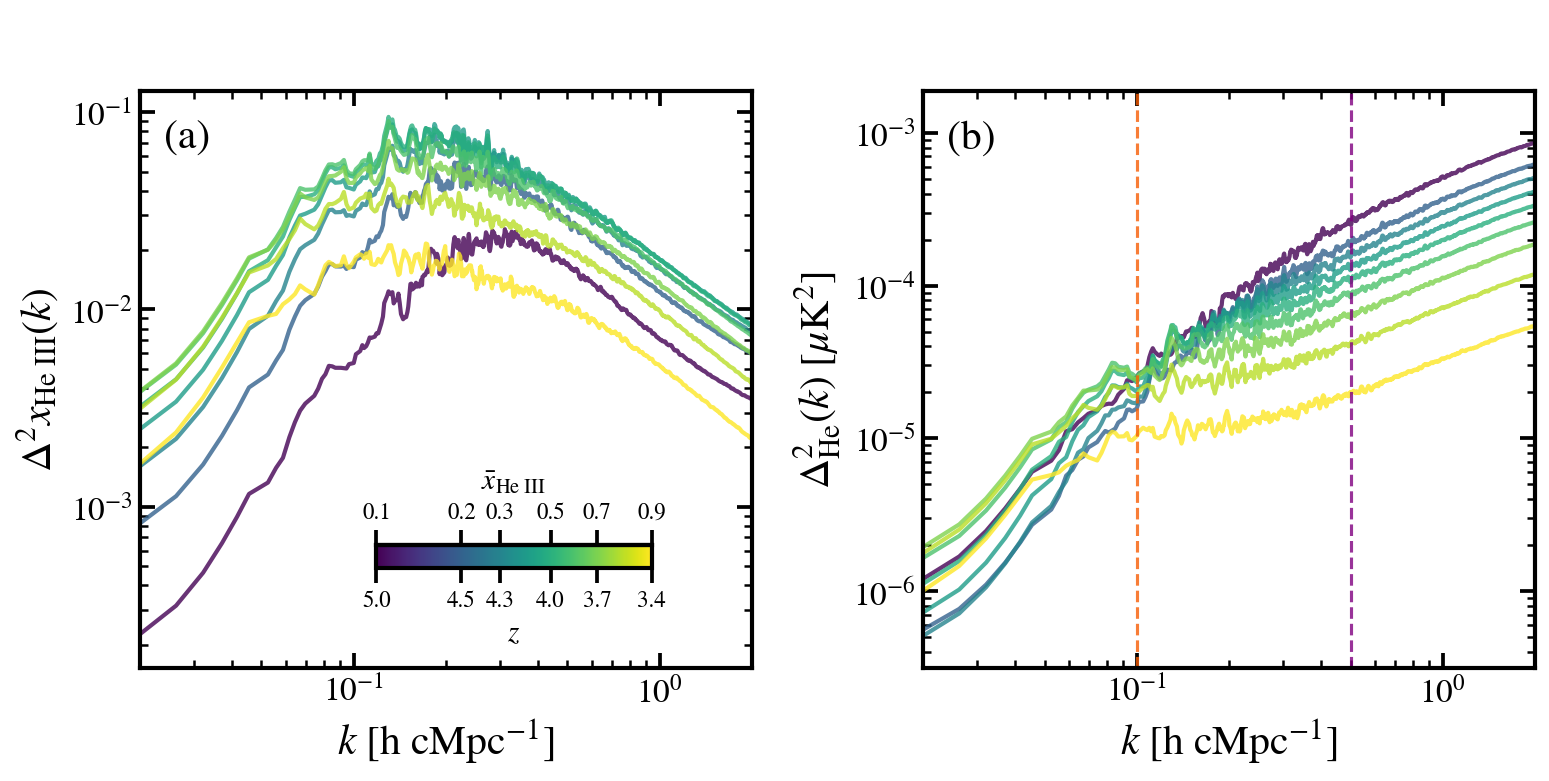
\includegraphics[width=\linewidth]{figs/ps_helium.png}
    \par\medskip
    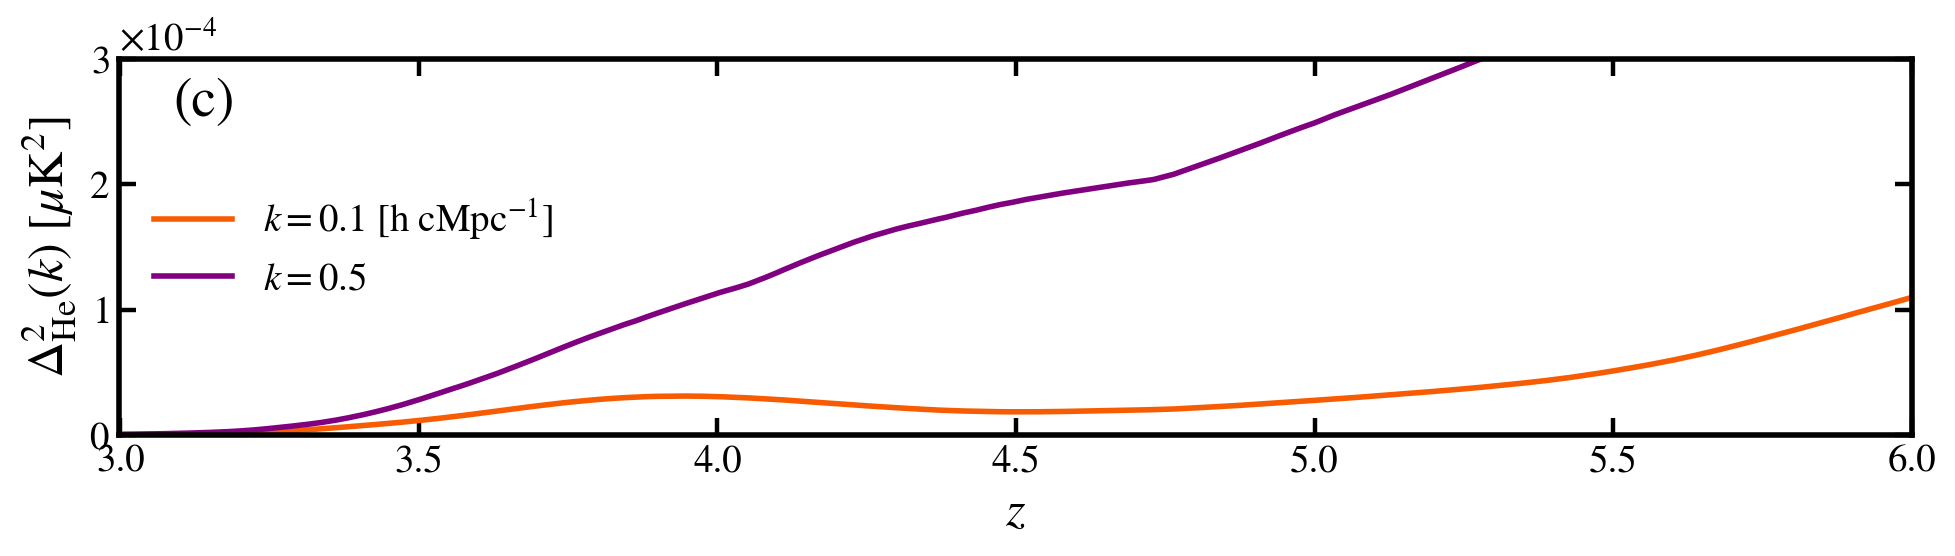
\includegraphics[width=\linewidth]{figs/ps_helium_z.png}
    \caption{Redshift evolution of the dimensionless power spectra for the doubly ionized helium fraction $\Delta^2_{x_\mathrm{He\,III}}(k)$ (panel a) and the 3.46\,cm brightness temperature $\Delta^2_\mathrm{He}(k)$ (panel b). Colors indicate redshift from $z = 5$ (dark purple) to $z = 3.4$ (yellow), corresponding to a global ionized fraction $\bar{x}_\mathrm{He\, III}$ increasing from $0.1$ to $0.9$. Vertical dashed lines in panel (b) mark $k = 0.1$ (orange) and $0.5\,h\,\mathrm{cMpc}^{-1}$ (purple). Panel (c) shows the redshift evolution of $\Delta^2_\mathrm{He}(k)$ at these two representative wavenumbers from $z = 6$ to $z = 3$.}
    \label{fig:ps_helium}
\end{figure*}

The orange dashed curve shows the \textsc{thesan-1} result at $k = 0.5\,h\,\mathrm{cMpc}^{-1}$, which broadly follows the same qualitative evolution as \lumina: a rise from the density-dominated regime, a peak associated with the characteristic bubble scale, and a subsequent decline as reionization completes. However, the two simulations differ in the precise timing of this evolution. The \textsc{thesan-1} power peaks at $z \approx 7.8$, earlier than \lumina's peak at $z \approx 7$, reflecting the fact that \textsc{thesan-1}'s ionization history proceeds more rapidly, shifting the epoch at which the characteristic bubble size matches $\sim 2.5/k_\mathrm{peak}$ to higher redshift. The peak amplitude is comparable between the two ($\Delta^2 \sim 14$--$15\ \mathrm{mK}^2$), suggesting that the power at the characteristic bubble scale is broadly similar despite differences in the underlying source models. At $z \lesssim 7$, both simulations converge toward a common declining trend as the neutral fraction approaches zero, reinforcing that the late-stage power suppression is a generic feature of reionization completion rather than a model-specific prediction.


Comparing these theoretical predictions against future instrument sensitivity limits provides a concrete observational context. In Figure \ref{fig:ps_hydro} (c), the red and blue dashed curves with triangles show the $2\sigma$ thermal noise power spectrum of SKA-Low \citep[][]{Barry2022} assuming 100 hours of integration at $k = 0.5$ and $0.1\,h\,\mathrm{cMpc}^{-1}$ respectively, while the blue dotted curve with squares shows the corresponding LOFAR-HBA \citep[][]{vanHaarlem2013} sensitivity at $k = 0.1\,h\,\mathrm{cMpc}^{-1}$ for 1000 hours. Across the bulk of the reionization epoch, the predicted signal lies above the SKA-Low sensitivity at both wavenumbers, and \lumina exceeds the LOFAR 1000-hour sensitivity at $k = 0.1\,h\,\mathrm{cMpc}^{-1}$ for $5.8 \lesssim z \lesssim 7.3$, indicating that the signal at these scales should in principle be detectable with future deep integrations.


\subsubsection{Helium power spectrum}



Figure \ref{fig:ps_helium} presents the redshift evolution of the dimensionless power spectra for the doubly ionized helium fraction $\Delta^2_{x_\mathrm{He\,III}}(k)$ (panel a) and the 3.46\,cm brightness temperature $\Delta^2_\mathrm{He}(k)$ (panel b), spanning $z = 3.4$ to $z = 5$. Panel (c) tracks the redshift evolution of $\Delta^2_\mathrm{He}(k)$ at two representative wavenumbers marked by vertical dashed lines in panel (b).


Panel (a) traces the spatial fluctuations of the \ion{He}{3} fraction, revealing the topology of quasar-driven helium reionization. At early times ($z \approx 5$, $\bar{x}_\mathrm{He\,III} = 0.1$), the power spectrum already exhibits a peak at $k \approx 0.3\,h\,\mathrm{cMpc}^{-1}$, indicating the presence of isolated \ion{He}{3} bubbles surrounding the first luminous quasar sources. As helium reionization advances, the amplitude of the power spectrum increases and the peak systematically shifts toward lower $k$, reflecting the expansion and merger of \ion{He}{3} regions into larger coherent ionized structures, analogous to the peak migration observed during hydrogen reionization. The fluctuation amplitude reaches its maximum near the midpoint of helium reionization before rapidly declining as the \ion{He}{3} field approaches uniformity by $z \approx 3.4$. In Section~\ref{sec:bubble}, we quantify how these power spectrum peak scales track the evolving \ion{He}{3} bubble size distribution across redshift. Compared to hydrogen reionization, the characteristic scales are systematically larger, reflecting the rare, highly clustered quasar population and the long mean free paths of the hard ionizing photons driving helium reionization.

Panel (b) presents the observable 3.46\,cm brightness temperature power spectrum, with amplitudes in the $10^{-6}\text{--}10^{-3}\, \mu\mathrm{K}^2$ regime. Because the IGM is generally not thermally saturated for the 3.46\,cm transition, the signal retains sensitivity to the spatially varying spin temperature in addition to the \ion{He}{2} fraction and the underlying density field, rather than tracing the ionization topology alone. A characteristic shoulder emerges around $k \approx 0.1\,h\,\mathrm{cMpc}^{-1}$, set by the size of the growing \ion{He}{3} regions. Early on, these expanding \ion{He}{3} bubbles carve zero-signal holes into the surrounding \ion{He}{2} emission, sharpening the contrast and building power on the scale of the bubbles. Later, once most of the \ion{He}{2} has been converted to \ion{He}{3}, little emitting gas remains, so the contrast fades and the power falls at all $k$ as helium reionization completes.


Our predicted amplitude lies between previous estimates. At $k = 0.1\,h\,\mathrm{cMpc}^{-1}$ and $z \approx 4$, we find $\Delta^2_\mathrm{He} \approx 3\times10^{-5}\, \mu\mathrm{K}^2$. At the same scale and redshift, \citet{Spina2025}, who compute the helium spin temperature self-consistently, obtain $\Delta^2_\mathrm{He} \approx 10^{-6}\ \mu\mathrm{K}^2$. \citet{Basu2026} obtain $\Delta^2_\mathrm{He} \approx 6\times10^{-5}\ \mu\mathrm{K}^2$ at $z = 4.18$ when the spin temperature is set by collisional coupling alone, and $\approx 3\times10^{-2}\ \mu\mathrm{K}^2$ in the fully coupled limit $T_S^\mathrm{He} = T_\mathrm{gas}$. Our result is thus close to their collisional estimate and far below the saturated limit, consistent with the weak global coupling discussed in Section~\ref{sec:global}, but roughly 30 times above the self-consistent estimate of \citet{Spina2025}. We attribute this difference primarily to the stronger local coupling in \lumina, where the spatially resolved \ion{He}{2} Ly$\alpha$ background raises $T_S^\mathrm{He}$ above $T_\gamma$ in the vicinity of luminous sources, whereas \citet{Spina2025} adopt a uniform UV background. Differences in helium reionization timing and in the sampling of rare quasars within the larger \lumina volume may also contribute.


%The right panel presents the 3.46\,cm brightness temperature power spectrum. The amplitude of this signal is on the order of $\mu\text{K}^2$, roughly six orders of magnitude lower than the hydrogen 21\,cm power spectrum ($\sim \text{mK}^2$). Unlike the \ion{He}{3} ionization field power spectrum (left panel), which exhibits a prominent peak associated with quasar-driven bubble morphology, the 3.46\,cm signal closely follows the underlying matter power spectrum. Even at $z=5$, when the volume-averaged \ion{He}{3} fraction is $\sim 0.1$, the IGM is already significantly heated ($T_K \gg T_\gamma$). In this regime, the brightness temperature becomes effectively independent of $T_S$ and primarily traces the local gas density. As a result, the 3.46\,cm fluctuations reflect the underlying matter distribution rather than the topology of \ion{He}{3} ionization fronts, since earlier stellar populations have already established a pervasive \ion{He}{2} background throughout the IGM.


%Consequently, the 3.46\,cm signal acts as an anti-tracer to the \ion{He}{3} fraction. The signal is produced exclusively by \ion{He}{2}; therefore, as reionization progresses and \ion{He}{2} is converted into \ion{He}{3}, expanding holes are carved into the 3.46\,cm emission map. This anti-correlation culminates at $z \to 3$, where the complete double-ionization of helium eradicates the remaining \ion{He}{2}, causing the 3.46\,cm signal to vanish entirely. While the intrinsic faintness of this transition makes detection extremely difficult, the evolution of the power spectra demonstrates its unique value as a statistical probe of both the morphology of AGN-driven reionization and the thermal state of the high-redshift IGM.


Panel (c) tracks the temporal evolution of $\Delta^2_\mathrm{He}(k)$ at $k = 0.1$ (orange) and $0.5\,h\,\mathrm{cMpc}^{-1}$ (purple), evolving from early times at high redshift toward the completion of helium reionization at low redshift. At early times ($z \approx 6$), both modes exhibit relatively strong power as the widespread \ion{He}{2} emission tracks the underlying density and ionization field. As helium reionization progresses toward lower redshift, the overall power declines as expanding \ion{He}{3} regions deplete the \ion{He}{2} reservoir. The two modes evolve differently during this transition: the $k = 0.5\,h\,\mathrm{cMpc}^{-1}$ mode decreases gradually, while the $k = 0.1\,h\,\mathrm{cMpc}^{-1}$ mode develops a local enhancement near $z \approx 3.9$. This temporary boost occurs when the growing \ion{He}{3} regions reach scales comparable to $R_\mathrm{ion} \sim 2.5/k_\mathrm{peak}$, enhancing the low-$k$ fluctuations before the \ion{He}{2} reservoir becomes substantially depleted. Similar to the hydrogen case, this staggered evolution is consistent with an inside-out reionization scenario in which small ionized regions form first before merging into larger coherent structures. Unlike hydrogen reionization, however, the helium signal is not thermally saturated, and the singly ionized helium forms shells around the growing \ion{He}{3} regions rather than simply tracing neutral gas. These differences smear out the sharp anti-correlation between density and ionization that drives the pronounced transitional dip in the 21\,cm signal, so the helium modes show only a shallow plateau rather than a deep dip.  Finally, both modes approach zero by $z \approx 3$ as the \ion{He}{2} fraction is fully converted into \ion{He}{3} and the 3.46\,cm signal disappears.

%\section{Result}



\subsection{Bispectrum} \label{sec:bispectrum}


%While the VID and power spectrum capture complementary aspects of the 21\,cm and 3.46\,cm signals, they do not fully characterize their spatial structure. In particular, both statistics are insensitive to the phase correlations that encode the morphology of ionized and heated regions. During Cosmic Dawn and the EoR, localized processes such as X-ray heating and the growth of ionized bubbles generate highly non-Gaussian spatial features that require higher-order statistics to describe.


The bispectrum, which measures correlations between three Fourier modes forming closed triangular configurations, directly encodes phase information \citep[e.g.,][]{Lewis2011, Hutter2020a}. Through its sensitivity to the scale and geometry of these configurations, the bispectrum provides a particularly powerful probe of the characteristic sizes, shapes, and spatial distribution of ionized structures. This makes it uniquely suited to capture non-Gaussian topological information that lower-order statistics alone cannot access.

While the 21\,cm bispectrum has been extensively used to characterize reionization morphologies \citep[e.g.,][]{Majumdar2018, Hutter2020a, Acharya2024}, previous work assumes a saturated spin temperature ($T_\mathrm{S} = T_\mathrm{K}$). This simplification neglects spatial variations in $T_\mathrm{S}$, obscuring the role of local thermal history during reionization. Additionally, the 3.46\,cm helium bispectrum remains unexplored. Here, we address these gaps by self-consistently calculating $T_\mathrm{S}$ evolution and presenting the first predictions for the 3.46\,cm helium bispectrum.


Mathematically, the bispectrum $B(\mathbf{k}_1, \mathbf{k}_2, \mathbf{k}_3)$ represents the three-point correlation function in Fourier space, given by \citep[][]{Watkinson2017}:

\begin{equation}
    B(\mathbf{k}_1, \mathbf{k}_2, \mathbf{k}_3) = \frac{\langle \Delta(\mathbf{k}_1) \,\Delta(\mathbf{k}_2)\,\Delta(\mathbf{k}_3) \rangle}{(2\pi)^3 \,\delta^\mathrm{D}(\mathbf{k}_1 + \mathbf{k}_2 + \mathbf{k}_3)} \, ,
\end{equation}
where $\Delta(\mathbf{k})$ is the fractional signal fluctuation and $\delta^\mathrm{D}$ enforces closed triangle configurations ($\mathbf{k}_1 + \mathbf{k}_2 + \mathbf{k}_3 = \mathbf{0}$).

We follow \citet{Watkinson2017} and use the normalized bispectrum, which cancels out power spectrum contributions to yield a dimensionless probe of non-Gaussianity:

\begin{equation}
    \tilde{B}(\mathbf{k}_1, \mathbf{k}_2, \mathbf{k}_3) = \frac{B(\mathbf{k}_1, \mathbf{k}_2, \mathbf{k}_3)}{\sqrt{(k_1 \, k_2 \, k_3)^{-1} P(k_1) \, P(k_2) \, P(k_3)}} \, .
\end{equation}



%Because the bispectrum depends on correlations among three wavevectors, its full parameter space is intrinsically high-dimensional and difficult to interpret directly. To build physical intuition, we parameterize the Fourier triangle using the cosine of the opening angle ($\theta$) between two wavevectors, $\mathbf{k}_1$ and $\mathbf{k}_2$, which uniquely determines the triangle geometry for a fixed set of side lengths. This geometric parameterization allows us to isolate different physical contributions to the signal.

Because the bispectrum spans a high-dimensional parameter space, direct physical interpretation is challenging. To analyze the bispectrum, we fix $k_1$ and $k_2$ and parameterize the triangle geometry by the opening angle $\theta$ between $\mathbf{k}_1$ and $\mathbf{k}_2$. The closed-triangle condition sets the magnitude of the third wavevector:

\begin{equation}
    k_3 = \sqrt{k_1^2 + k_2^2 + 2k_1k_2\cos\theta} \, .
\end{equation}
Varying $\theta$ isolates distinct triangle shapes that probe different physical processes during reionization.

In particular, we focus on two representative triangle configurations designed to probe both scale-dependent and cross-scale mode coupling:


\begin{itemize}
    %\item \textbf{Equilateral configuration ($k_1 = k_2 = k_3 = k$):} We evaluate this configuration over $0.15 \leq k \leq 2 \,\mathrm{cMpc}^{-1}$ to isolate the scale dependence of the non-Gaussian signal. This configuration is particularly sensitive to the characteristic sizes of heated regions and ionized bubbles, as it probes structures at a single spatial scale.

%  ($k_1 = k_2 = 0.05$--$1.5\,h\,\mathrm{cMpc}^{-1}$)

    \item \textbf{Isosceles configuration:} By fixing $k_1 = k_2$ and varying $\theta$, this family probes mode coupling across scales spanning characteristic bubble growth. It systematically traces three reionization regimes: (\textit{i}) early bubble formation in large-scale overdensities, (\textit{ii}) intermediate bubble percolation, and (\textit{iii}) late-stage residual neutral islands. % The selected $k$-range encompass the characteristic scales of ionized bubble growth throughout reionization. By testing multiple distinct $k$-modes within this range, we systematically map the shape dependence of the bispectrum across three physically distinct regimes: (i) the early stage, where isolated bubbles are forming within large-scale overdensities; (ii) the intermediate stage, where bubbles have grown sufficiently large to overlap and percolate into surrounding voids; and (iii) the late stage, where only residual neutral islands persist within an otherwise ionized IGM. Together, these configurations allow us to track how the non-Gaussian structures of the hydrogen and helium signals evolve as reionization progresses.

    %  ($k_1 = k_2/2 = 0.2-0.4\,h\,\mathrm{cMpc}^{-1}$)
    \item \textbf{Non-isosceles configuration:} Breaking $k_1 = k_2$ symmetry by setting $k_2 = 2k_1$ samples two distinct physical scales simultaneously. This probes cross-scale coupling between intermediate bubble growth and late-stage island fragmentation, breaking degeneracies inherent to symmetric configurations. %By deliberately breaking the $k_1 = k_2$ symmetry of the isosceles family, this configuration simultaneously probes two physically distinct scales within a single triangular template. The chosen scale ratio ($k_2 = 2k_1$) places the two independent legs at physical scales differing by a factor of two, spanning the characteristic scales of intermediate bubble growth and late-stage neutral island fragmentation identified in the isosceles analysis. This asymmetric sampling therefore provides complementary morphological information to the isosceles configuration, probing the coupling between structures at different scales that would otherwise appear degenerate in a symmetric triangle family.
\end{itemize}


Once the triangle shape is specified, varying $\cos\theta$ sweeps the bispectrum through three geometric limits that target distinct spatial morphologies:


\begin{itemize}
    \item \textbf{Stretched limit ($\cos\theta \to 1$):} As $\theta \to 0^\circ$, wavevectors align collinearly ($k_3 \approx k_1 + k_2$), where a fully stretched triangle ($\cos\theta = 1$) specifically probes plane-like spatial fluctuations at the smallest scales ($r_3 \sim \pi/k_3$). %At scales smaller than the characteristic bubble size, it samples inter-bubble neutral gas (positive bispectrum). As $r_3$ expands to resolve coherent ionized bubbles, the bispectrum turns negative. The transition angle $\cos\theta_t$ (where $k_{3,t} = k\sqrt{2(1 + \cos\theta_t)}$) marks this sign flip, directly measuring the characteristic bubble radius ($R_\mathrm{ion} \approx \pi/k_{3,t}$).

    %As the opening angle approaches ${\sim}\,0^\circ$, the wavevectors become nearly collinear with $k_3 \approx k_1 + k_2$, such that $k_3$ reaches its maximum wavenumber for a given $(k_1, k_2)$ pair and probes the smallest physical scales ($r_3 \sim \pi/k_3$) accessible within that triangular configuration. At this limit, depending on the chosen $k_1 = k_2$ scale, the template may probe scales smaller than the characteristic bubble radius. In this case, it samples the neutral gas occupying the inter-bubble medium rather than resolving individual bubbles as coherent structures, driving the bispectrum to positive values. However, as $\cos\theta$ decreases away from unity and $r_3$ grows toward the characteristic ionized bubble radius $R_\mathrm{ion}$, the template begins to capture ionized bubbles as coherent below-average concentrations in the 21\,cm and 3.46\,cm brightness temperature and ionization fields, causing the bispectrum to become negative. This ``sign flip'' occurs at the transition configuration $\cos\theta_t$, where $k_{3,t} = k\sqrt{2(1 + \cos\theta_t)}$, providing a direct geometric measurement of the characteristic bubble size ($R_\mathrm{ion} \approx \pi/k_{3,t}$) at a given epoch of reionization.

    \item \textbf{Equilateral limit ($\cos\theta \approx -0.5$):} With three equal legs ($\theta \sim 120^\circ$), this limit is maximally sensitive to spherical structures. It produces a strongly negative signal for isolated ionized bubbles during early reionization, while tracing spherical residual neutral islands at late times. % At an opening angle of $\sim120^\circ$, all three legs of the isosceles triangle are of equal length, making this configuration optimally sensitive to isotropic, spherical structures. During the early stages of reionization, the equilateral bispectrum reaches its most negative value, tracing the spherical geometry of isolated ionized bubbles that imprint localized low-signal regions in both the ionization and brightness temperature fields of hydrogen and helium. In the late stages, the equilateral configuration continues to mark the extremum of the bispectrum across triangle scales. Its sign is scale-dependent, remaining negative at small scales while becoming positive at large scales. In both regimes, the equilateral limit consistently captures the spherical geometry of the residual neutral islands that survive as the last pockets of un-ionized gas within large-scale underdense regions.


    \item \textbf{Squeezed limit ($\cos\theta \to -1$):} As $\theta \to 180^\circ$ ($k_3 \to 0$), the collapsed triangle isolates cross-scale mode coupling, quantifying how small-scale power ($k_1 \approx k_2$) is modulated by the large-scale background field $k_3$. A positive squeezed bispectrum indicates that small-scale ionized structures cluster preferentially within large-scale overdensities (characteristic of inside-out reionization). %As the opening angle approaches $\sim180^\circ$, the two short wavevectors point in nearly opposite directions, forcing $k_3 \to 0$ and collapsing the triangle into a degenerate configuration. This limit directly probes cross-scale mode coupling, quantifying how small-scale structures traced by $k_1 \approx k_2$ are modulated by the large-scale density field traced by $k_3$. In the context of reionization, a positive squeezed bispectrum indicates that small-scale ionized structures cluster preferentially within large-scale overdensities, consistent with inside-out reionization, whereas a negative signal reflects the subsequent anti-correlation, where overdense regions have been more fully ionized and thus appear as depressions in the 21\,cm and 3.46\,cm brightness temperature fields.
\end{itemize}


All bispectra presented in this work are computed using the \textsc{bifft} package \citep[][]{Scoccimarro2015,Sefusatti2016,Watkinson2017}.


\subsubsection{Hydrogen isosceles bispectrum}

\begin{figure*}[!t]
    \centering
    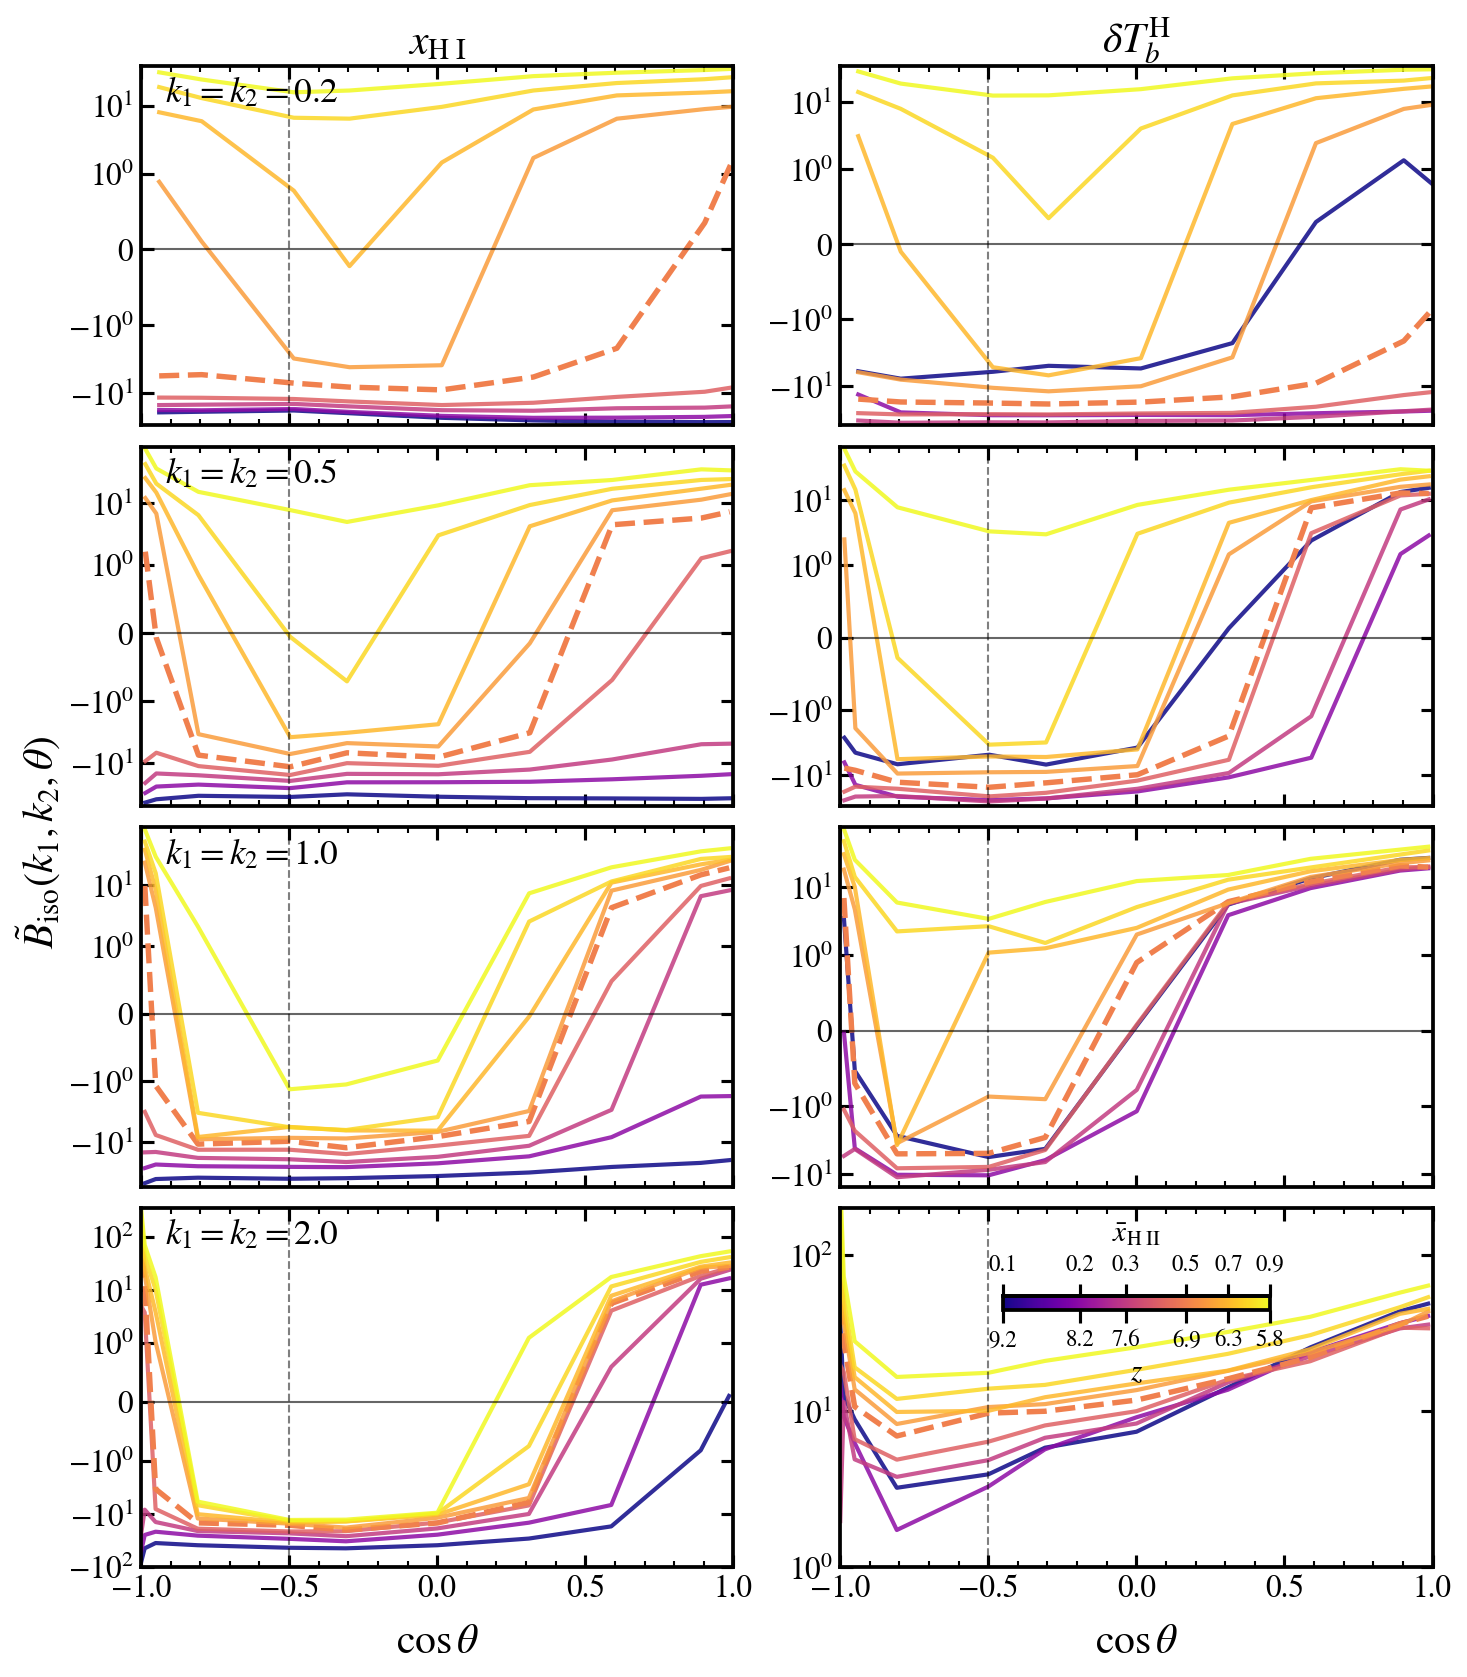
\includegraphics[width=\textwidth]{figs/bispec_H_iso.png}
    \caption{Redshift evolution of the isosceles bispectrum $B_\mathrm{iso}(k, k, k)$ for the neutral hydrogen fraction $x_\mathrm{H\,I}$ (left panels) and the 21\,cm brightness temperature $\delta T_\mathrm{b}^\mathrm{H}$ (right panels), evaluated at four fixed $k$-modes: $k_1 = k_2 = 0.2$, $0.5$, $1.0$, and $2.0\,h\,\mathrm{cMpc}^{-1}$ (top to bottom). Colors indicate redshift from $z = 9.2$ (dark blue) to $z = 5.8$ (yellow), corresponding to $\bar{x}_\mathrm{H\, II}$ increasing from $0.1$ to $0.9$, with the dashed curve marking the midpoint ($\bar{x}_\mathrm{H\, II} = 0.5$). The vertical dashed line marks the equilateral configuration at $\cos\theta = -0.5$.}
    \label{fig:bispec_H_iso}
\end{figure*}


Figure \ref{fig:bispec_H_iso} shows the redshift evolution of the isosceles bispectra for both the neutral hydrogen fraction ($x_\mathrm{H\,I}$; left panels) and the 21\,cm brightness temperature ($\delta T_\mathrm{b}^\mathrm{H}$; right panels). Rows display progressively smaller spatial scales, from $k_1 = k_2 = 0.2\,h\,\mathrm{cMpc}^{-1}$ (top) to $2.0\,h\,\mathrm{cMpc}^{-1}$ (bottom). Color-coded curves span $z = 9.2 \to 5.8$, corresponding to global ionization fractions $\bar{x}_{\mathrm{H\,II}} = 0.1 \to 0.9$, with orange dashed lines highlighting the half-ionized epoch ($\bar{x}_{\mathrm{H\,II}} = 0.5$). Direct comparison between $x_\mathrm{H\,I}$ and $\delta T_\mathrm{b}^\mathrm{H}$ quantifies how spin temperature, density fluctuations, and line-of-sight velocity distortions alter the observed signal relative to the intrinsic ionization morphology. Across these four scales, we track the sign, amplitude, and shape evolution of the bispectrum to identify configurations that most cleanly encode ionized bubble growth and neutral island evolution.

%The redshift evolution of the isosceles bispectra for both the neutral hydrogen fraction ($x_\mathrm{H \,I}$; left panels) and the 21\,cm brightness temperature ($\delta T^\mathrm{H}_\mathrm{b}$; right panels) is shown in Figure \ref{fig:bispec_H_iso}. To systematically track how spatial correlations depend on the physical size of the underlying structures, the rows display this evolution across progressively smaller spatial scales, with the two fixed legs of the Fourier triangle ranging from $k_1 = k_2 = 0.14 \,h\,\mathrm{cMpc}^{-1}$ (top row) to $1.5 \,h\,\mathrm{cMpc}^{-1}$ (bottom row). Within each panel, the curves are color-coded by redshift, spanning from $z = 9.2$ (dark blue) to $z = 5.8$ (yellow). This range directly corresponds to the global ionized hydrogen fraction ($\bar{x}_{\mathrm{H \ II}}$) increasing from $0.1$ up to $0.9$. To explicitly mark the morphological tipping point (going from mostly neutral to mostly ionized) of the epoch of reionization, the bispectra at the half-ionized epoch ($\bar{x}_{\mathrm{H\ II}} = 0.5$) are highlighted as dashed lines. Comparing $x_\mathrm{H\,I}$ directly against $\delta T_b^\mathrm{H}$ quantifies the deviation between the observable signal and the underlying neutral gas morphology. Unlike the ionization field, the brightness temperature carries additional dependences on the spin temperature, baryon overdensity, and line-of-sight peculiar velocity, each of which can distort the bispectrum relative to the intrinsic $x_\mathrm{H\,I}$ distribution. Across the four $k$-scales, we track how the sign, amplitude, and shape dependence of the bispectrum evolve as reionization progresses, with the goal of identifying which triangular configurations most cleanly encode the growth of ionized bubbles and the emergence of large-scale neutral islands.

The left panels of Figure \ref{fig:bispec_H_iso} reveal a topological sign reversal in the $x_\mathrm{H\,I}$ isosceles bispectrum. During early reionization ($\bar{x}_\mathrm{H\,II} < 0.5$), expanding \ion{H}{2} regions form below-average neutral concentrations in a largely neutral IGM, driving a negative bispectrum across all configurations. Near the half-ionized epoch ($\bar{x}_\mathrm{H\,II} \approx 0.5$), declining contrast between bubbles and the background suppresses this negative amplitude. Past this threshold ($\bar{x}_\mathrm{H\,II} > 0.5$), the topology inverts: the continuous neutral medium fragments into isolated neutral islands that act as above-average concentrations in an ionized background, turning the bispectrum positive. This positive signal strengthens as reionization completes and contrast increases, peaking at large scales ($k_1 = k_2 = 0.2\,h\,\mathrm{cMpc}^{-1}$) where the triangle template cleanly encompasses the shrinking neutral islands as coherent structures.

%The left panels of Figure \ref{fig:bispec_H_iso} reveal a sign reversal in the $x_\mathrm{H\ I}$ bispectrum that traces the topological transition of the IGM. During the first half of reionization ($\bar{x}_\mathrm{H\ II} < 0.5$), the bispectrum is predominantly negative across all configurations and $k$-modes. In this regime, the cosmic volume is largely neutral, and expanding \ion{H}{2} regions act as below-average concentrations relative to the mean neutral fraction, driving the bispectrum to negative values. As reionization approaches its midpoint, the global neutral fraction declines, reducing the contrast between ionized bubbles and the neutral background and causing the negative amplitude to decrease. Once reionization surpasses the half-ionized threshold ($\bar{x}_\mathrm{H\ II} > 0.5$), the topology inverts: the bulk of the volume becomes ionized, and the previously continuous neutral cosmic web undergoes progressive fragmentation into isolated, neutral islands. These residual structures now constitute above-average neutral fractions relative to the ionized background, driving the bispectrum to positive values. As the global ionized fraction increases further, the contrast between the residual neutral regions and the surrounding ionized medium intensifies, driving continued growth in the positive amplitude, most pronounced at $k_1 = k_2 = 0.14\,h\,\mathrm{cMpc}^{-1}$. At this scale the triangular template is larger than the individual neutral islands, so it captures them as coherent above-average neutral concentrations, yielding a positive bispectrum. Once the neutral phase has fragmented to scales well below the template, this positive signal persists and strengthens as the contrast between the shrinking islands and the surrounding ionized medium grows.

At higher $k$-modes, the isosceles bispectrum exhibits strong shape dependence driven by local geometry rather than the global neutral fraction alone. Across intermediate configurations, the high-$k$ bispectrum remains predominantly negative, featuring a distinct minimum near $\cos\theta \approx -0.5$ (the ``equilateral trough''). Because equilateral triangles probe isotropic features, the persistence of this trough across scales confirms that \ion{H}{2} regions expand as relatively compact, spherical bubbles. Positive signals emerge only at the angular extremes: the stretched limit ($\cos\theta \to 1$) traces plane-like anisotropic neutral structures between bubbles, while the squeezed limit ($\cos\theta \to -1$) reflects cross-scale modulation, demonstrating that small-scale neutral fluctuations are environmentally enhanced within large-scale neutral regions.


%While the global topological inversion is clearly visible at large scales ($k_1 = k_2 = 0.14\,h\,\mathrm{cMpc}^{-1}$), the bispectrum exhibits a pronounced shape dependence at higher $k$-modes, where the physical size of the Fourier triangles becomes comparable to that of the local ionizing structures. In this regime, the specific geometry of ionized and neutral regions directly dictates the bispectrum amplitude, rather than the global neutral fraction alone. Most prominently, the small-scale (high $k$-mode) bispectrum remains predominantly negative across a wide range of intermediate triangular configurations. It exhibits a distinct global minimum near $\cos\theta \approx -0.5$, marked by the vertical dotted line, which we refer to as the equilateral trough. Since the equilateral configuration is optimally sensitive to isotropic, spherical structures, the persistence of this trough across multiple $k$-modes confirms that the dominant \ion{H}{2} regions expand as relatively compact, roughly spherical bubbles throughout reionization. The bispectrum transitions to positive values at the two extremes of the angular sweep, though through distinct physical mechanisms. In the stretched limit ($\cos\theta \to 1$), the signal tracks the anisotropic, plane-like structures of the surviving neutral cosmic web between ionized bubbles. In contrast, as the configuration approaches the squeezed limit ($\cos\theta \to -1$), the bispectrum measures how small-scale neutral structure is modulated by the large-scale neutral field. The positive squeezed signal shows that small-scale neutral fluctuations are enhanced where the large-scale neutral fraction is high; that is, the surviving neutral gas is environmentally clustered rather than uniformly distributed. %This modulation is consistent with inside-out reionization, the neutral gas that persists longest resides in the matter-underdense regions that reionize last.


% as established in the literature \citep[e.g.,][]{Hutter2020},

Beyond tracing geometry, the isosceles bispectrum's scale dependence provides a quantitative proxy for characteristic bubble sizes. The sign-flip angle $\cos\theta_t$ marks the transition from positive inter-bubble neutral gas to negative coherent ionized regions, directly yielding the \ion{H}{2} radius via $R_\mathrm{ion} \approx \pi/k_{3,t}$ (where $k_{3,t} = k\sqrt{2(1 + \cos\theta_t)}$). For example, at $k_1 = k_2 = 2.0\,h\,\mathrm{cMpc}^{-1}$ and $z = 9.2$, the sign flip is already present, indicating an early bubble size of $R_\mathrm{ion} \sim 0.8\,h^{-1}\,\mathrm{cMpc}$. As reionization progresses, $\cos\theta_t$ systematically shifts toward smaller $k_3$, corresponding to larger physical scales and tracking the bubble growth characteristic of inside-out reionization. A detailed quantitative analysis of this bubble size evolution is presented in Section \ref{sec:bubble}.


Because larger wavenumbers probe smaller physical scales ($r = \pi/k$), the sign flip appears within the resolved angular range only when the triangle scale is comparable to the typical size of the ionized regions. For each epoch, we therefore select $k_1 = k_2$ such that the sign flip falls in the stretched regime, $0.5 \leq \cos\theta \leq 1$, consistent with \citet{Hutter2020a}, who find the change from negative to positive values near $\cos\theta \approx 0.5$ when the triangle scale is comparable to the size of the ionized regions. In this range, $k_{3,t}$ lies between $\sqrt{3}\,k$ and $2k$, so the inferred radius, $\pi/(2k) \leq R_\mathrm{ion} \leq \pi/(\sqrt{3}\,k)$, is set mainly by the selected $k$, which decreases as the ionized regions grow.

%Beyond identifying specific geometric shapes, the scale dependence of the bispectrum provides a powerful quantitative proxy for the characteristic sizes of evolving ionized structures. The sign-flip point is the angular configuration at which the bispectrum transitions from positive to negative. It directly encodes the dominant \ion{H}{2} region size via $R_\mathrm{ion} \approx \pi/k_{3,t}$, where $k_{3,t}$ is the wavenumber of the third triangle leg at the zero-crossing. For example, at the highest probed scale ($k_1 = k_2 = 1.5\,h\,\mathrm{cMpc}^{-1}$), the sign flip is already visible at the earliest snapshots (e.g., $z = 9.2$, dark blue curves), indicating that the characteristic \ion{H}{2} region size at this epoch is already roughly of order $R_\mathrm{ion} \sim \pi/1.5 \approx 2\,h^{-1}\,\mathrm{cMpc}$. As reionization progresses, the sign-flip point systematically shifts toward lower $k_3$, reflecting the continuous growth of ionized bubbles. This provides a confirmation of the inside-out reionization scenario. We defer a detailed quantitative analysis of this bubble size evolution to Section \ref{sec:bubble}.

%Figure \ref{fig:bispec_H_iso} (a) shows the evolution of the equilateral bispectrum of the 21\,cm brightness temperature from $z \sim 10$ to $z \sim 5$, spanning the late stages of Cosmic Dawn and the EoR. The bispectrum traces the transition from heating-dominated fluctuations to ionization-driven structure. In particular, the sign of the bispectrum reflects the underlying topology of the brightness temperature field: negative values correspond to ionized regions appearing as cold voids embedded in a warmer neutral medium, while positive values arise from isolated neutral islands within an otherwise ionized IGM.

Shifting focus from the neutral fraction (left panels) to the observable 21\,cm brightness temperature (right panels of Figure \ref{fig:bispec_H_iso}), the $\delta T_\mathrm{b}^\mathrm{H}$  isosceles bispectrum overall mirrors the topological inversion, yet exhibits distinct departures driven by additional dependences on baryon overdensity $\delta_\mathrm{b}$ and spin temperature $T_\mathrm{S}^\mathrm{H}$ (Equation~\ref{eq:21cm}). Most notably, at $z = 9.2$ ($\bar{x}_\mathrm{H\,II} = 0.1$), the $\delta T_\mathrm{b}^\mathrm{H}$ bispectrum differs from its nearly flat $x_\mathrm{H\,I}$ counterpart because fluctuations in this predominantly neutral IGM are governed by density and thermal fields rather than ionization topology. Although X-ray heating has raised the mean spin temperature above the CMB by $z \approx 9$, heating remains incomplete, causing the thermal coupling prefactor $(1 - T_\gamma/T_\mathrm{S}^\mathrm{H})$ to vary from $\approx 0.37$ in cold voids to $\approx 1$ in heated overdensities. Because X-ray sources reside in overdense regions, $T_\mathrm{S}^\mathrm{H}$ correlates positively with $\delta_\mathrm{b}$, reinforcing density contrasts by suppressing emission from cold voids relative to hot, dense neutral peaks. Consequently, the $z \sim 9.2$ $\delta T_\mathrm{b}^\mathrm{H}$ bispectrum tracks the positive non-linear matter bispectrum, strongly amplified by these correlated thermal fluctuations.


%While the brightness temperature bispectrum (right panels of Figure \ref{fig:bispec_H_iso}) largely mirrors the overarching topological inversion seen in $x_\mathrm{H\ I}$, it exhibits several qualitatively distinct features driven by the additional dependence of $\delta T_\mathrm{b}^\mathrm{H}$ on the baryon overdensity $\delta_b$ and the spin temperature $T^\mathrm{H}_S$ (Equation~\ref{eq:21cm}).


%Most notably, at the earliest time ($z = 9.2$, $\bar{x}_\mathrm{H\,II} = 0.1$), the $\delta T_\mathrm{b}^\mathrm{H}$ bispectrum differs substantially from its nearly flat $x_\mathrm{H\,I}$ counterpart. At this stage, the IGM is almost entirely neutral, so the $\delta T_\mathrm{b}^\mathrm{H}$ fluctuations are primarily carried by the density and spin temperature fields. Although X-ray heating has already raised the mean spin temperature well above the CMB at $z \approx 9$, heating is not yet complete: the coupling prefactor $(1 - T_\gamma/T_S^\mathrm{H})$ ranges from $\approx 0.37$ in the coldest underdense voids to $\approx 1$ in the heated overdensities. Because $T_S^\mathrm{H}$ tracks $T_K$ and X-ray heating is concentrated near the overdense sources, this prefactor is positively correlated with $\delta_b$: it reinforces the density contrast by further suppressing the cold voids and leaving the hot, dense, still-neutral peaks at full amplitude. The $\delta T_\mathrm{b}^\mathrm{H}$ field at $z \sim 9.2$ therefore tracks the positive non-linear matter bispectrum, amplified by the correlated thermal modulation, and is strongly enhanced relative to the flat and negative $x_\mathrm{H\,I}$ signal.


As reionization progresses, two effects drive the $\delta T_\mathrm{b}^\mathrm{H}$ isosceles bispectrum to converge toward that of $x_\mathrm{H\,I}$. First, inside-out reionization preferentially ionizes the densest environments, converting high-emission regions into low-signal ionized bubbles. Second, ongoing heating warms the remaining voids, driving $(1 - T_\gamma/T_\mathrm{S}^\mathrm{H}) \to 1$, which suppresses thermal modulations so that ionization topology dominates. Nonetheless, the equilateral trough in $\delta T_\mathrm{b}^\mathrm{H}$ remains shallower than in $x_\mathrm{H\,I}$ due to a residual positive contribution from density fluctuations ($\delta_\mathrm{b}$). This offset fades only late in reionization as density and thermal variations become subdominant to the ionization contrast.


%As reionization progresses, two effects drive the $\delta T_\mathrm{b}^\mathrm{H}$ bispectrum toward the ionization fraction bispectrum. First, in our inside-out topology, the densest environments initially dominate the emission but are preferentially ionized early, becoming holes that suppress $\delta T_b^\mathrm{H}$. Second, continued heating warms the residual voids, so $(1 - T_\gamma/T^\mathrm{H}_S) \rightarrow 1$ throughout the IGM and the thermal modulation fades. The ionization field thereby begins to dominate, and the bispectrum morphology of $\delta T_\mathrm{b}^\mathrm{H}$ progressively converges toward that of $x_\mathrm{H\,I}$. However, relative to $x_\mathrm{H\,I}$, the $\delta T_b^\mathrm{H}$ trough is shallower. This offset is set by the residual positive density contribution near the equilateral configuration and shrinks late in reionization as the density and thermal contributions become subdominant.


At the smallest probed scale ($k_1 = k_2 = 2.0\,h\,\mathrm{cMpc}^{-1}$), the $\delta T_\mathrm{b}^\mathrm{H}$ isosceles bispectrum remains positive across all redshifts, opposing the strongly negative $x_\mathrm{H\,I}$ signal. This divergence is driven by deeply non-linear matter clustering. Because inside-out reionization ionizes overdensities first ($\delta_\mathrm{b} > 0$ where $x_\mathrm{H\,I} < \bar{x}_\mathrm{H\,I}$), density and neutral gas are spatially anti-correlated. In the brightness temperature field ($\delta T_\mathrm{b}^\mathrm{H} \propto x_\mathrm{H\,I}(1+\delta_\mathrm{b})$), the strong, positive non-linear matter bispectrum overcomes the negative ionization contribution, keeping $\delta T_\mathrm{b}^\mathrm{H}$ positive across all triangle geometries throughout reionization.


%Finally, at the highest-wavenumber configuration ($k_1 = k_2 = 1.5\,h\,\mathrm{cMpc}^{-1}$, probing $r = \pi/1.5 \approx 2\,h^{-1}\,\mathrm{cMpc}$), the $\delta T_\mathrm{b}^\mathrm{H}$ bispectrum remains positive across all redshifts even though the $x_\mathrm{H\,I}$ bispectrum is strongly negative at the same scale. This sign reversal is not driven by the ionization topology, which would imprint the negative $x_\mathrm{H\,I}$ signal. Instead it is driven by the $(1+\delta_b)$ weighting: at these deeply non-linear scales the positive matter bispectrum dominates the negative ionization contribution, rendering $\delta T_b^\mathrm{H}$ positive across all configurations and throughout reionization.


%The opposing statistical trends between the $x_\mathrm{H\,I}$ and $\delta T_\mathrm{b}^\mathrm{H}$ bispectra are consistent with an inside-out reionization scenario. In this picture, the earliest ionized regions correspond to positive matter overdensities ($\delta_b > 0$) while simultaneously having a lower neutral fraction than average ($x_\mathrm{H\,I} < \bar{x}_\mathrm{H\,I}$), so that dense regions and neutral gas are spatially anti-correlated. This anti-correlation propagates into the observable brightness temperature through the coupling $\delta T_b^\mathrm{H} \propto x_\mathrm{H\,I}(1+\delta_b)$, where the density weighting reinforces the signal in dense neutral gas and suppresses it in dense ionized regions, causing the $\delta T_\mathrm{b}^\mathrm{H}$ bispectrum to evolve differently from the neutral fraction bispectrum.


%This anti-correlation is directly transferred to the observable brightness temperature through the coupling $\delta T_b^\mathrm{H} \propto x_\mathrm{H\,I}(1+\delta_b)$, causing the $\delta T_\mathrm{b}^\mathrm{H}$ bispectrum to evolve differently from the neutral fraction bispectrum. The effect is most evident at intermediate scales ($k_1 = k_2 = 0.4$--$0.8\,h\,\mathrm{cMpc}^{-1}$), where the negative trough of the brightness temperature bispectrum occupies a narrower range in $\cos\theta$ than the corresponding $x_\mathrm{H\,I}$ bispectrum. Together, these signatures support a reionization topology in which dense regions ionize first and later expand into the surrounding IGM, a picture further quantified through the bubble size analysis presented in Section \ref{sec:bubble}.

\subsubsection{Hydrogen non-isosceles bispectrum}

\begin{figure*}[!t]
    \centering
    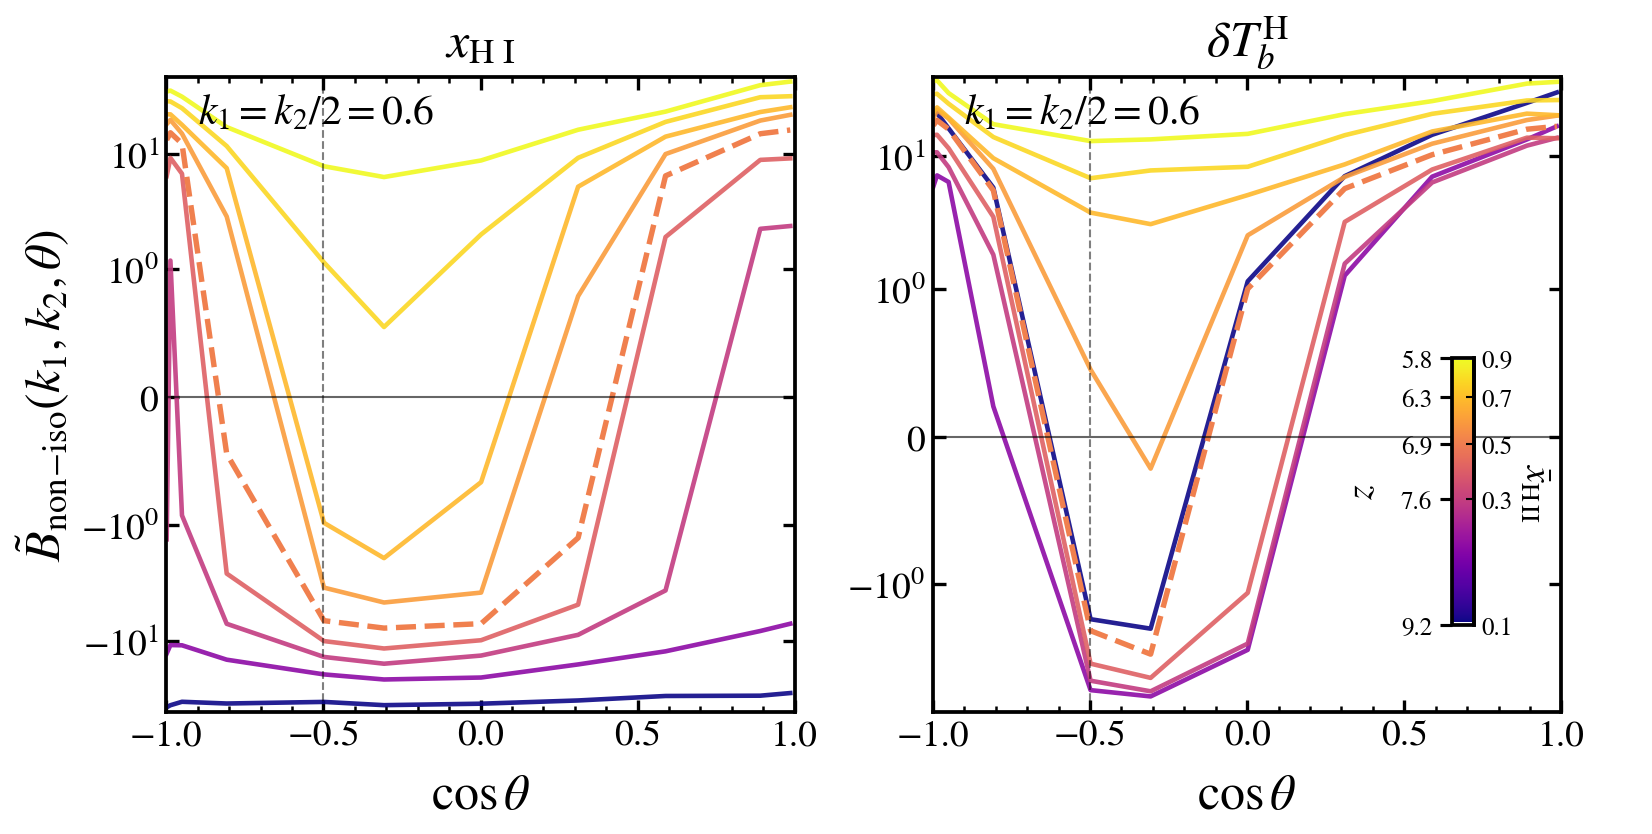
\includegraphics[width=\textwidth]{figs/non_iso_H.png}
    \caption{Redshift evolution of the non-isosceles bispectrum $B_\mathrm{non\text{-}iso}(k_1, k_2, k_3)$ for the neutral hydrogen fraction $x_\mathrm{H\,I}$ (left panel) and the 21\,cm brightness temperature $\delta T_\mathrm{b}^\mathrm{H}$ (right panel), evaluated at the fixed configuration $k_1 = k_2/2 = 0.6\,h\,\mathrm{cMpc}^{-1}$. Colors and dashed curve follow the same convention as Figure~\ref{fig:bispec_H_iso}, with the vertical dashed line marking the configuration at $\cos\theta = -0.5$.}
    \label{fig:non_iso_H}
\end{figure*}


Moving beyond isosceles configurations to capture cross-scale coupling, we evaluate a non-isosceles bispectrum with $k_1 = k_2/2 = 0.6\,h\,\mathrm{cMpc}^{-1}$. The fixed base legs correspond to $r_1 \approx 5.2\,h^{-1}\,\mathrm{cMpc}$ and $r_2 \approx 2.6\,h^{-1}\,\mathrm{cMpc}$, bridging the scales of intermediate bubble growth and late-stage island fragmentation. Sweeping the opening angle $\theta$ varies the third leg $k_3$ monotonically from $0.6\,h\,\mathrm{cMpc}^{-1}$ at the folded limit ($\cos\theta \to -1$) to $1.8\,h\,\mathrm{cMpc}^{-1}$ at the stretched limit ($\cos\theta \to 1$), probing physical scales from $\sim 5.2$ down to $\sim 1.7\,h^{-1}\,\mathrm{cMpc}$. Because $k_1 \neq k_2$, this asymmetric geometry contains neither equilateral nor squeezed limits, providing complementary morphological information on how cross-scale coupling evolves throughout reionization.


%While the isosceles bispectrum maps the morphological evolution at individual characteristic scales, it cannot simultaneously probe the coupling between two physically distinct scales within a single triangular configuration. To quantify this cross-scale mode coupling, we evaluate a non-isosceles bispectrum defined by $k_1 = k_2/2 = 0.4\,h\,\mathrm{cMpc}^{-1}$. This choice is motivated by the isosceles analysis: the two independent legs correspond to physical scales of $r_1 \sim \pi/k_1 \approx 8\,h^{-1}\,\mathrm{cMpc}$ and $r_2 \sim \pi/k_2 \approx 4\,h^{-1}\,\mathrm{cMpc}$, which span the characteristic scales of intermediate bubble growth and late-stage neutral island fragmentation identified earlier, making this configuration optimally suited for probing the coupling between these two physically distinct regimes. By sweeping through the opening angle $\theta$, the third leg $k_3$ scans monotonically from $k_3 = |k_2 - k_1| = 0.4\,h\,\mathrm{cMpc}^{-1}$ at the folded limit ($\cos\theta \to -1$) to $k_3 = k_1 + k_2 = 1.2\,h\,\mathrm{cMpc}^{-1}$ at the stretched limit ($\cos\theta \to 1$). Unlike the isosceles family, this configuration shows neither a squeezed ($k_3 \to 0$) nor an equilateral limit due to $k_1 \neq k_2$; the two base scales $r_1$ and $r_2$ stay fixed while only the third leg $k_3$ varies from $\sim 8$ to $\sim 3\,h^{-1}\,\mathrm{cMpc}$. This asymmetric triangle geometry provides complementary morphological information to the isosceles configurations, enabling a direct measurement of how cross-scale coupling evolves as reionization progresses.

Figure \ref{fig:non_iso_H} shows the redshift evolution of the non-isosceles bispectrum for $x_\mathrm{H\,I}$ (left) and $\delta T_\mathrm{b}^\mathrm{H}$ (right). Both fields recover the global topological inversion observed in the isosceles case, transitioning from negative at high redshift to positive as reionization completes. Key deviations from the isosceles case appear at the angular extremes, where the three wavevectors become nearly co-linear. Late in reionization ($z \lesssim 7$), the signal at the folded limit ($\cos\theta \to -1$) turns strongly positive. Consequently, this positive rise reflects direct cross-scale coupling between $r_1$ and $r_2$ as neutral gas fragments into isolated islands, rather than modulation by a distinct large-scale mode.


%Figure \ref{fig:non_iso_H} presents the redshift evolution of the non-isosceles bispectrum for $x_\mathrm{H\ I}$ (left panel) and $\delta T_\mathrm{b}^\mathrm{H}$ (right panel), using the same color and redshift convention as Figure \ref{fig:bispec_H_iso}. Both panels recover the global topological inversion seen in the isosceles case, with the bispectrum transitioning from predominantly negative values at high redshift to positive values as reionization completes. The notable deviations from the isosceles case emerge at the extremes of the angular sweep, where the wavevectors $k_1$, $k_2$, and $k_3$ become nearly parallel or anti-parallel. As reionization progresses ($z \lesssim 7$), the signal at the folded limit ($\cos\theta \to -1$) rises to strongly positive values. Because $k_1 \neq k_2$, this limit is folded rather than squeezed: all three legs remain comparable in magnitude, so the positive signal reflects the coupling of neutral structure across the two base scales $r_1$ and $r_2$ rather than modulation by a distinct large-scale mode. The growth of this positive amplitude tracks the same topological inversion identified in the isosceles analysis, as the neutral field fragments into above-average concentrations late in reionization.


%The notable deviations from the isosceles case emerge at the collinear extremes of the angular sweep, where the wavevectors $k_1$, $k_2$, and $k_3$ become nearly parallel or anti-parallel. As reionization progresses ($z \lesssim 7$), the signal at the squeezed limit ($\cos\theta \to -1$) rises to strongly positive values. This indicates that small-scale neutral structures are preferentially located within large-scale underdense environments, consistent with the inside-out reionization scenario established in the isosceles analysis.


The stretched limit ($\cos\theta \to 1$, where $k_3 \to 1.8\,h\,\mathrm{cMpc}^{-1}$) also exhibits a pronounced positive rise. At this configuration, the third leg probes scales of $r_3 \approx 1.7\,h^{-1}\,\mathrm{cMpc}$, which fall below the characteristic bubble radius during intermediate and late reionization (Figure \ref{fig:bubble_size}). Rather than resolving individual bubbles as coherent voids, the template samples the neutral inter-bubble gas, driving the non-isosceles bispectrum positive. Together, the positive signals at both collinear extremes confirm that late-time residual neutral gas is non-randomly distributed, maintaining cross-scale spatial coherence.


%The stretched limit ($\cos\theta \to 1$, where $k_3 \to 1.2\,h\,\mathrm{cMpc}^{-1}$) exhibits a pronounced positive rise. At this configuration, the third leg of the triangle probes physical scales of $r_3 \sim \pi/k_3 \approx 3\,h^{-1}\,\mathrm{cMpc}$, which is smaller than the characteristic ionized bubble radius at intermediate-to-late stages of reionization (Figure \ref{fig:bubble_size}). The triangular template, therefore, no longer resolves individual bubbles as coherent below-average concentrations; instead, it probes the neutral gas occupying the inter-bubble medium, which constitutes an above-average concentration relative to the ionized background and drives the bispectrum to positive values.


Unlike the symmetric equilateral minimum at $\cos\theta \approx -0.5$ in the isosceles case, the non-isosceles bispectrum exhibits a visibly asymmetric trough shifted toward intermediate configurations (vertical dashed line). This shift stems from the broken leg symmetry ($k_1 \neq k_2$), which causes large and small modes to respond differently to the same underlying ionization structures. Consequently, the coupling between large ionized regions ($r_1 \approx 5.2\,h^{-1}\,\mathrm{cMpc}$) and smaller neutral features ($r_2 \approx 2.6\,h^{-1}\,\mathrm{cMpc}$) becomes inherently scale-dependent and asymmetric.


%The non-isosceles geometry probes the coupling between two unequal scales within a single triangle. Unlike the isosceles bispectrum, which exhibits a symmetric global minimum near $\cos\theta \approx -0.5$ (corresponding to an equilateral configuration), the non-isosceles configuration produces a visibly asymmetric trough. As highlighted by the vertical dashed line in the figure, the minimum is shifted toward intermediate triangle configurations. This asymmetry arises geometrically from the broken $k_1 = k_2$ symmetry of the triangle itself, causing the large- and small-scale modes to respond differently to the same ionization structures. Consequently, the statistical coupling between large ionized regions ($r_1 \approx 8\,h^{-1}\,\mathrm{cMpc}$) and smaller neutral structures ($r_2 \approx 4\,h^{-1}\,\mathrm{cMpc}$) becomes distinctly scale-dependent and asymmetric. %The non-isosceles bispectrum thereby accesses cross-scale information not available from an isosceles triangle, complementing the isosceles analysis.

%The non-isosceles geometry further reveals the breakdown of perfect spherical symmetry across interacting spatial scales. Unlike the isosceles bispectrum, which exhibits a symmetric global minimum near $\cos\theta \approx -0.5$ (corresponding to an equilateral configuration), the non-isosceles configuration produces a visibly asymmetric trough. As highlighted by the vertical dashed line in the figure, the minimum is shifted toward intermediate triangle configurations. Part of this asymmetry arises purely geometrically from the broken $k_1 = k_2$ symmetry of the triangle itself, causing the large- and small-scale modes to respond differently to the same ionization structures. However, this effect might reflect the intrinsically inhomogeneous nature of reionization, in which ionization fronts expand non-uniformly through the anisotropic density structure of the cosmic web. Consequently, the statistical coupling between large ionized regions (e.g., $r_1 \approx 12\,\mathrm{cMpc}$) and smaller neutral structures (e.g., $r_2 \approx 6\,\mathrm{cMpc}$) becomes distinctly scale-dependent and asymmetric. Ultimately, the non-isosceles bispectrum is uniquely sensitive to this cross-scale mode coupling, capturing essential morphological information regarding the ionization topology that cannot be resolved by the symmetric isosceles configuration alone.

Comparing the $x_\mathrm{H\,I}$ and $\delta T_\mathrm{b}^\mathrm{H}$ non-isosceles bispectra highlights the coupled roles of ionization, density, and thermal structure during reionization. As in the isosceles case, the $z = 9.2$ curve deviates at early times because fluctuations are driven by dense, heated, partially neutral regions. At later times, density coupling partially dilutes the pure ionization signal, producing a shallower negative trough in $\delta T_\mathrm{b}^\mathrm{H}$ due to incomplete anti-correlation. Conversely, because inside-out reionization ionizes overdensities first, this positive density weighting accelerates the transition to positive values, causing the sign flip to occur earlier in $\delta T_\mathrm{b}^\mathrm{H}$ than in $x_\mathrm{H\,I}$. Together, the two fields offer complementary windows into the EoR: $x_\mathrm{H\,I}$ isolates the ionization topology, whereas $\delta T_\mathrm{b}^\mathrm{H}$ encodes its interaction with matter clustering and gas thermodynamics.


%Comparing the $x_\mathrm{H\ I}$ and $\delta T_\mathrm{b}^\mathrm{H}$ bispectra further highlights the coupled roles of ionization, density, and thermal structure during reionization. Consistent with the isosceles analysis, the $z = 9.2$ curve in the right panel deviates from the other high-redshift curves because the earliest stages of reionization are still dominated by overdense heated regions that have not yet become fully ionized. At this epoch, the brightness temperature receives simultaneous contributions from the neutral fraction, baryon overdensity, and spatially varying spin temperature through $\delta T_b^\mathrm{H} \propto x_\mathrm{H\ I}(1+\delta_b)(1-T_\gamma/T^\mathrm{H}_S)$. Consequently, dense regions that are both hotter and only partially ionized generate strong localized fluctuations that amplify the bispectrum signal relative to the neutral fraction field alone. Beyond this early-time anomaly, the $\delta T_\mathrm{b}^\mathrm{H}$ bispectrum exhibits a sharp negative trough and steeper positive enhancements at the collinear extremes relative to the $x_\mathrm{H\ I}$ bispectrum. The brightness temperature bispectrum therefore reflects the combined effect of ionization, density structure, and spin temperature rather than mirroring the neutral fraction bispectrum alone. The coupling with $\delta_b$ partially dilutes the pure ionization signal, producing a noticeably shallower negative trough in the $\delta T_\mathrm{b}^\mathrm{H}$ bispectrum relative to the $x_\mathrm{H\ I}$ bispectrum, since the density field is not perfectly correlated with the ionization field and their cross-correlation partially cancels the clean negative ionization signature. However, this same density coupling causes the sign flip to occur earlier in reionization for the $\delta T_b^\mathrm{H}$ bispectrum than for the $x_\mathrm{H\,I}$ bispectrum. Overdense regions are preferentially ionized first in an inside-out scenario, and their positive density-weighted signal accelerates the transition to positive bispectrum values. Together, the $x_\mathrm{H\ I}$ bispectrum and the $\delta T_\mathrm{b}^\mathrm{H}$ bispectrum therefore provide complementary windows into the EoR: the former offers a cleaner measure of ionization topology, while the latter encodes the additional coupling between reionization morphology, the baryon density field, and the thermal state of the gas.


\subsubsection{Helium isosceles bispectrum}

\begin{figure*}[!t]
    \centering
    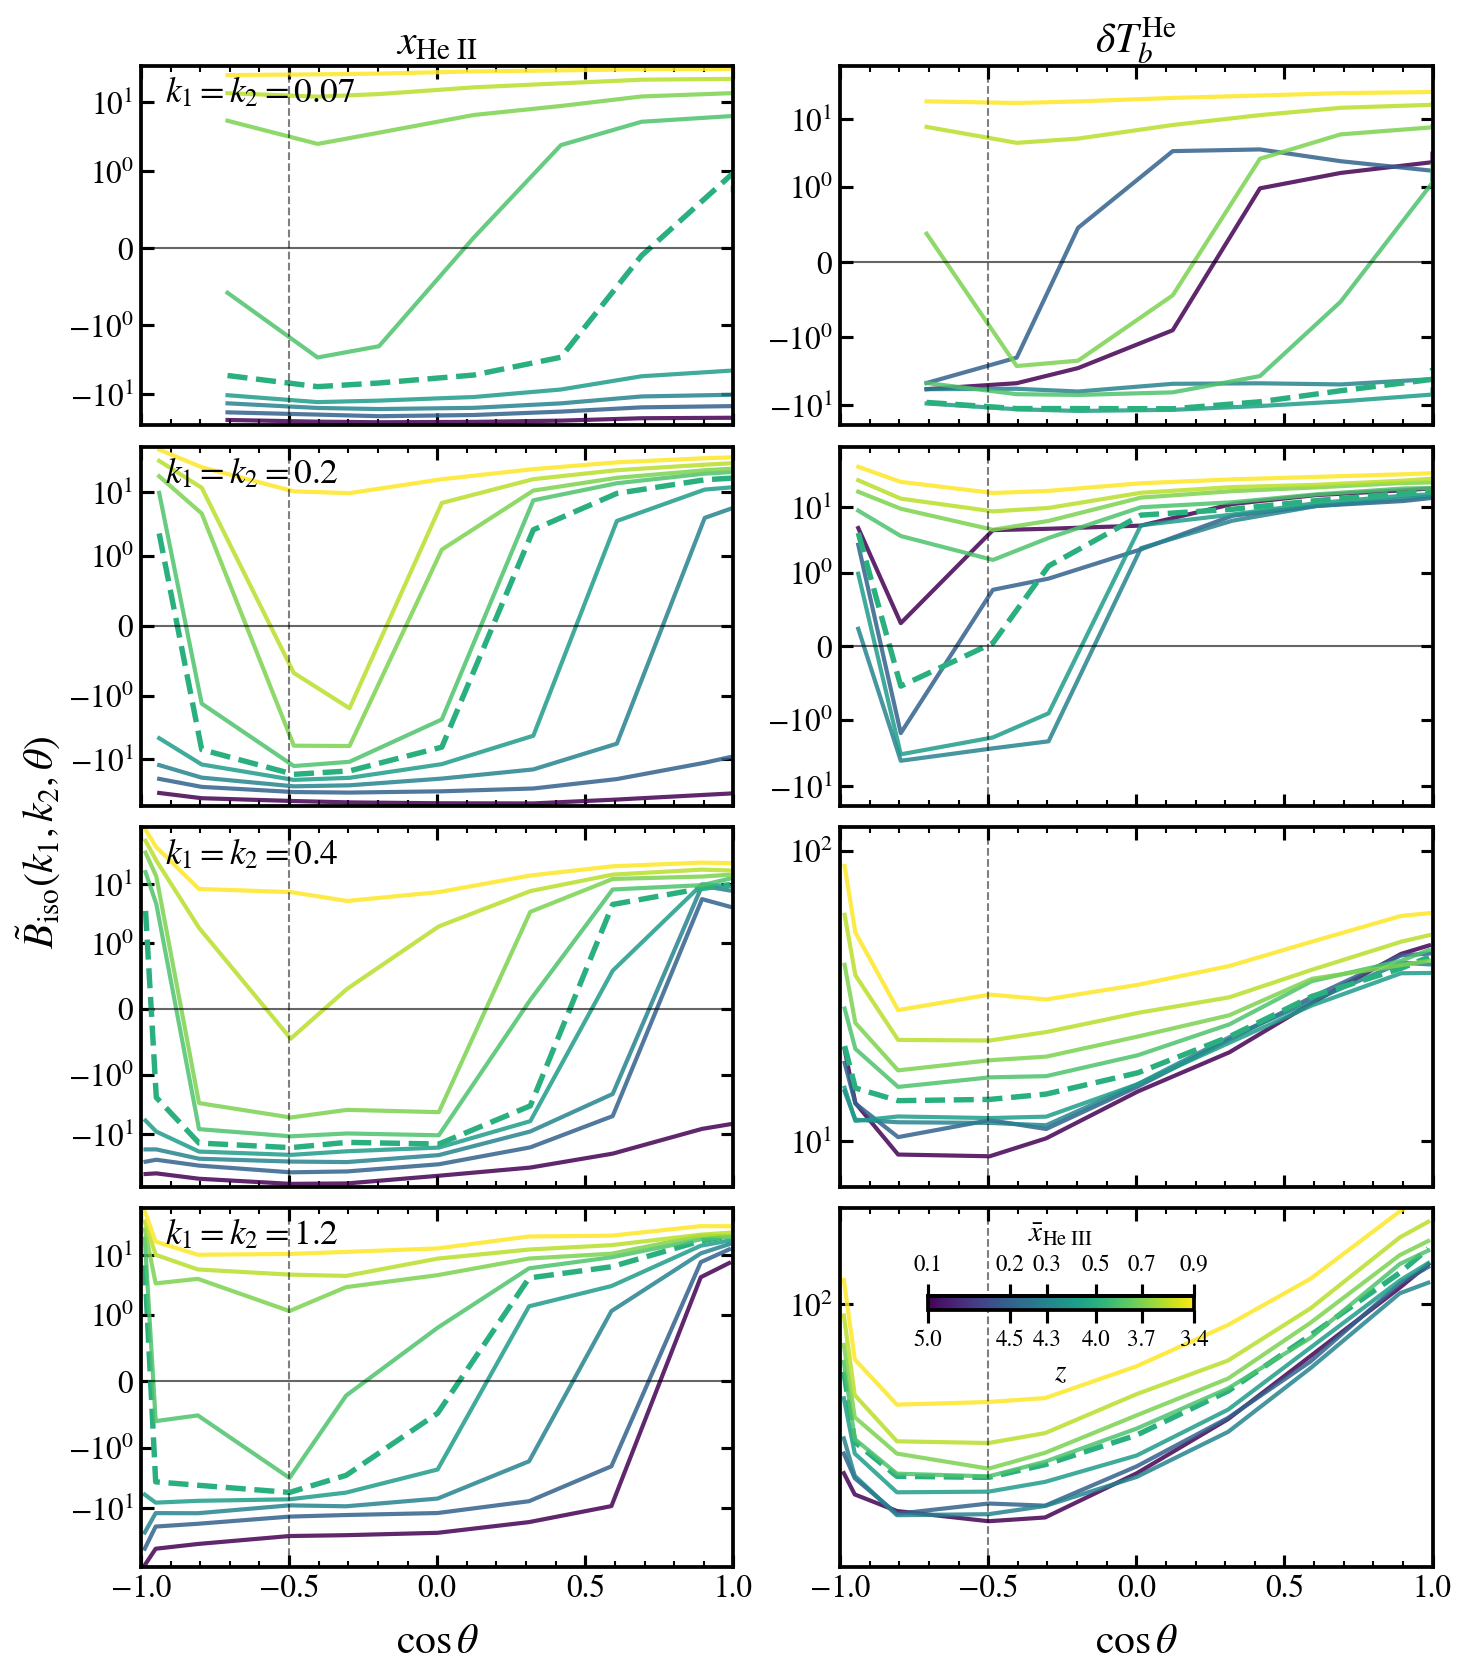
\includegraphics[width=\textwidth]{figs/bispec_He_iso.png}
    \caption{Redshift evolution of the isosceles bispectrum $B_\mathrm{iso}(k, k, k)$ for the singly ionized helium fraction $x_\mathrm{He\,II}$ (left panels) and the 3.46\,cm brightness temperature $\delta T_\mathrm{b}^\mathrm{He}$ (right panels), evaluated at four fixed $k$-modes: $k_1 = k_2 = 0.07$, $0.2$, $0.4$, and $1.2\,h\,\mathrm{cMpc}^{-1}$ (top to bottom). Colors indicate redshift from $z = 5$ (dark purple) to $z = 3.4$ (yellow), corresponding to $\bar{x}_\mathrm{He\,III}$ increasing from $0.1$ to $0.9$, with the dashed curve marking the midpoint ($\bar{x}_\mathrm{He\,III} = 0.5$). Note that the right panels at $k_1 = k_2 = 0.4$ and $1.2\,h\,\mathrm{cMpc}^{-1}$ is displayed on a logarithmic scale, reflecting the entirely positive $\delta T_\mathrm{b}^\mathrm{He}$ bispectrum at these scales. The vertical dashed line marks the equilateral configuration at $\cos\theta = -0.5$.}
    \label{fig:bispec_He_iso}
\end{figure*}

Figure \ref{fig:bispec_He_iso} presents the redshift evolution of the isosceles bispectrum for $x_\mathrm{He\,II}$ (left panels) and $\delta T_\mathrm{b}^\mathrm{He}$ (right panels) across four scales from $k_1 = k_2 = 0.07$ to $1.2\,h\,\mathrm{cMpc}^{-1}$. Curves are color-coded from $z = 5$ ($\bar{x}_\mathrm{He\,III} = 0.1$) to $z = 3.4$ ($\bar{x}_\mathrm{He\,III} = 0.9$), with the midpoint ($\bar{x}_\mathrm{He\,III} = 0.5$) highlighted as a green dashed curve. While $x_\mathrm{He\,II}$ broadly mirrors the global topological inversion seen in hydrogen, its detailed features reflect the distinct physics of helium reionization. Driven by hard quasar spectra rather than stellar UV, helium reionization produces large, sharp-edged \ion{He}{3} bubbles anchored to massive overdensities. Furthermore, $x_\mathrm{He\,II}$ does not trace neutral gas; it maps an intermediate ionization state that forms overdense shells around expanding \ion{He}{3} regions, as \ion{He}{1} is singly ionized in outer radiation fields before being doubly ionized near the central sources. This shell geometry and strong quasar halo bias fundamentally alter the non-Gaussian bispectrum relative to the hydrogen case.


%Figure \ref{fig:bispec_He_iso} presents the redshift evolution of the isosceles bispectrum for the singly ionized helium fraction $x_\mathrm{He\ II}$ (left panels) and the 3.46\,cm brightness temperature $\delta T_\mathrm{b}^\mathrm{He}$ (right panels), across four fixed $k$-scales ranging from $k_1 = k_2 = 0.05\,h\,\mathrm{cMpc}^{-1}$ (top row) to $0.7\,h\,\mathrm{cMpc}^{-1}$ (bottom row). Curves are color-coded by redshift from $z = 5$ (dark purple) to $z = 3.4$ (yellow), corresponding to a global \ion{He}{3} fraction $\bar{x}_\mathrm{He\ III}$ increasing from $0.1$ to $0.9$, with the midpoint ($\bar{x}_\mathrm{He\ III} = 0.5$) highlighted as a dashed curve. The $x_\mathrm{He\,II}$ bispectrum broadly mirrors the topological inversion seen in the hydrogen case, transitioning from predominantly negative values at early times to positive values as reionization completes. However, it exhibits several physically distinct features that reflect the different nature of helium reionization. Unlike hydrogen reionization, which is driven by stellar UV photons producing relatively diffuse \ion{H}{2} regions, helium reionization is driven by the harder ionizing spectra of quasars, which produce larger, harder-edged \ion{He}{3} bubbles concentrated within the most massive overdensities of the cosmic web. Crucially, $x_\mathrm{He\ II}$ does not simply track neutral gas as $x_\mathrm{H\ I}$ does; instead, it traces an intermediate ionization state that forms overdense shells surrounding the growing \ion{He}{3} regions, as \ion{He}{1} is first singly ionized in the outskirts of quasar radiation fields before being doubly ionized into \ion{He}{3} in the harder radiation interior. This shell-like geometry of the \ion{He}{2} field, combined with the strong large-scale bias of quasar host halos, alters the non-Gaussian bispectrum signature relative to the hydrogen case.

The left panels of Figure \ref{fig:bispec_He_iso} show a global sign reversal in the $x_\mathrm{He\,II}$ isosceles bispectrum, paralleling the topological transition seen in hydrogen reionization. At early times ($z \sim 5$), when the IGM is dominated by \ion{He}{2}, growing quasar-driven \ion{He}{3} regions act as below-average voids in $x_\mathrm{He\,II}$, driving the bispectrum strongly negative across most configurations. As the helium reionization midpoint approaches ($\bar{x}_\mathrm{He\,III} = 0.5$), contrast diminishes and the negative amplitude attenuates. Beyond $\bar{x}_\mathrm{He\,III} > 0.5$, the topology inverts: the \ion{He}{2} medium fragments into isolated structures within a \ion{He}{3} background, turning the bispectrum positive. Throughout this evolution, a persistent negative trough near $\cos\theta \approx -0.5$ confirms that quasar-driven \ion{He}{3} regions expand as quasi-spherical bubbles under isotropic AGN radiation.

%The left panels of Figure \ref{fig:bispec_He_iso} reveal a global sign reversal in the $x_\mathrm{He\ II}$ bispectrum that broadly parallels the topological transition seen in the hydrogen case. At early times ($z \sim 5$), when the IGM is overwhelmingly dominated by \ion{He}{2}, the emergence of quasar-driven \ion{He}{3} regions creates below-average concentrations within the $x_\mathrm{He\ II}$ field, driving the bispectrum to strongly negative values across most of the configurations and $k$-modes. As the \ion{He}{3} volume fraction increases to 0.5, the contrast between the singly ionized and fully ionized regions diminishes, causing the negative amplitude to attenuate toward the midpoint of helium reionization. Once the half-ionized threshold is surpassed ($\bar{x}_\mathrm{He\ III} > 0.5$), the topology inverts: the previously pervasive \ion{He}{2} medium undergoes progressive fragmentation into isolated structures embedded within a highly ionized \ion{He}{3} background, driving the bispectrum to positive values. Beyond this global evolution, the bispectrum exhibits a pronounced shape dependence that encodes the specific morphology of the \ion{He}{3} bubbles. Across intermediate triangular configurations, the bispectrum maintains a distinct negative trough near $\cos\theta \approx -0.5$. This confirms that the quasar-driven \ion{He}{3} regions expand predominantly as quasi-spherical bubbles, consistent with the hard, isotropic radiation fields of AGN sources.

Past the helium reionization midpoint ($\bar{x}_\mathrm{He\,III} > 0.5$), the isosceles bispectrum turns positive at both angular extremes through distinct physical mechanisms. In the stretched limit ($\cos\theta \to 1$), this positivity reflects the sheet-like geometry of \ion{He}{2} shells surrounding \ion{He}{3} bubbles, enhanced by the strong bias of quasar sources. In the squeezed limit ($\cos\theta \to -1$), the positive signal demonstrates that small-scale \ion{He}{2} fluctuations are amplified within regions of high large-scale \ion{He}{2} fraction, confirming that singly ionized helium is environmentally clustered rather than uniformly distributed.

%Past the midpoint of helium reionization, the bispectrum turns positive at both extremes of the angular sweep, through distinct physical mechanisms. In the stretched limit ($\cos\theta \to 1$), the signal is consistent with the sheet-like geometry of the \ion{He}{2} shells surrounding the \ion{He}{3} bubbles. This positivity reflects the strong bias of the quasar sources driving \ion{He}{3} growth. In contrast, as the configuration approaches the squeezed limit ($\cos\theta \to -1$), the bispectrum measures how small-scale \ion{He}{2} structure is modulated by the large-scale \ion{He}{2} field. The positive squeezed signal shows that small-scale \ion{He}{2} fluctuations are enhanced where the large-scale \ion{He}{2} fraction is high; that is, the singly ionized helium is environmentally clustered rather than uniformly distributed.


%The bispectrum transitions to positive values only at the collinear extremes of the angular sweep. Toward the stretched limit ($\cos\theta \to 1$), the signal tracks the neutral inter-bubble medium at scales smaller than the characteristic \ion{He}{3} bubble radius, consistent with the scale-matching argument established in the hydrogen analysis. The positive enhancement at the squeezed limit ($\cos\theta \to -1$) reflects strong cross-scale mode coupling. %It indicates that the residual \ion{He}{2} structures are not randomly distributed across the IGM but are preferentially concentrated in underdense voids. This is consistent with inside-out reionization, in which quasar-rich overdensities are ionized first, leaving \ion{He}{2} to survive longest in the most underdense regions.


As in the hydrogen analysis, the scale-dependent sign flip of the $x_\mathrm{He\,II}$ isosceles bispectrum yields the characteristic \ion{He}{3} bubble size via $R_\mathrm{ion} \approx \pi/k_{3,t}$. At the smallest probed scale ($k_1 = k_2 = 1.2\,h\,\mathrm{cMpc}^{-1}$), this sign flip is already present at $z \sim 5$, indicating $R_\mathrm{ion} \approx 1.4\,h^{-1}\,\mathrm{cMpc}$ (Section~\ref{sec:bubble}). %This exceeds the \ion{H}{2} bubble size at equivalent ionized fractions, consistent with hard, extended quasar radiation fields. Section \ref{sec:bubble} presents the full calibrated bubble-size evolution.

%The scale-dependent sign flip of the $x_\mathrm{He\,II}$ bispectrum encodes the characteristic \ion{He}{3} bubble size via $R_\mathrm{ion} \approx \pi/k_{3,t}$, as in the hydrogen analysis. At the smallest probed scale ($k_1 = k_2 = 0.7\,h\,\mathrm{cMpc}^{-1}$), the sign flip is already present at $z \sim 5$, giving $R_\mathrm{ion} \lesssim 4.5\,h^{-1}\,\mathrm{cMpc}$. This is larger than the \ion{H}{2} bubble size at comparable ionized fraction, consistent with the more extended radiation fields of quasar sources. We present the calibrated bubble-size evolution in Section \ref{sec:bubble}.


%The scale-dependent evolution of the $x_\mathrm{He\ II}$ bispectrum provides a quantifiable probe of the characteristic \ion{He}{3} bubble size throughout helium reionization, analogous to the sign-flip analysis applied to the hydrogen bispectrum. As established in that analysis, the sign-flip point encodes the dominant ionized region size. At the smallest probed scale ($k_1 = k_2 = 0.7\,h\,\mathrm{cMpc}^{-1}$), the sign flip is visible at the earliest snapshots. This indicates that the characteristic \ion{He}{3} bubble size at $z \sim 5$ is approximately $R_\mathrm{ion} \lesssim \pi/0.7 \approx 7\,\mathrm{cMpc}$. This is larger than the characteristic \ion{H}{2} bubble size at comparable ionized fractions, consistent with the more extended radiation fields of quasar sources. As helium reionization progresses, the sign-flip point systematically shifts toward lower wavenumbers, tracking the continuous growth and percolation of \ion{He}{3} regions across the IGM. At the terminal stages ($z \lesssim 3.5$), the bispectrum transitions to strongly positive values across all probed scales. This includes the smallest accessible scale ($k_1 = k_2 = 0.7\,h\,\mathrm{cMpc}^{-1}$), indicating that the residual \ion{He}{2} structures have been fragmented into compact islands smaller than $R_\mathrm{ion} \sim \pi/0.7 \approx 7\,\mathrm{cMpc}$. Together, the migration of the sign-flip point across the four $k$-modes provides a coherent, quantifiable timeline of \ion{He}{3} bubble growth throughout helium reionization, which we analyze in detail in Section \ref{sec:bubble}.




%Comparing the $x_\mathrm{He\,II}$ bispectrum (left) with the $\delta T_b^\mathrm{He}$ bispectrum (right) isolates how the density weighting of the brightness temperature reshapes the non-Gaussian signal relative to the intrinsic ionization field, since $\delta T_b^\mathrm{He} \propto x_\mathrm{He\,II}\,(1+\delta_b)\,(1-T_\gamma/T_S^\mathrm{He})$.

Comparing the $x_\mathrm{He\,II}$ (left) and $\delta T_\mathrm{b}^\mathrm{He}$ (right) isosceles bispectra reveals two helium-specific differences. First, \ion{He}{2} is an intermediate state forming shell geometries around expanding \ion{He}{3} regions, rather than tracing a simple binary topology. Second, $T_\mathrm{S}^\mathrm{He} \approx T_\gamma$ across most of the volume, suppressing the signal via $(1 - T_\gamma/T_\mathrm{S}^\mathrm{He}) \approx 0$. The 3.46\,cm brightness temperature is generated near luminous quasars, where intense radiation decouples $T_\mathrm{S}^\mathrm{He}$ from $T_\gamma$. Consequently, $\delta T_\mathrm{b}^\mathrm{He}$ samples a biased, overdense subset of the \ion{He}{2} field, shallowing its negative trough relative to $x_\mathrm{He\,II}$. At $k_1 = k_2 = 1.2\,h\,\mathrm{cMpc}^{-1}$, this density weighting lifts the trough entirely above zero, rendering the isosceles bispectrum positive across all configurations. Nevertheless, $\cos\theta \approx -0.5$ remains a local minimum, preserving the signature of spherically symmetric \ion{He}{2} shells.

%The comparison between the $x_\mathrm{He\,II}$ (left) and $\delta T_b^\mathrm{He}$ (right) bispectra follows the same logic as the hydrogen case, with two differences specific to helium. First, \ion{He}{2} is an intermediate ionization state, occupying shells between the \ion{He}{2} exterior and the \ion{He}{3} bubble interiors rather than tracing a simple two-phase topology. Second, both spin temperatures are computed self-consistently, but the \ion{He}{2} spin temperature departs from $T_\gamma$ only near active star-forming regions and AGN; over most of the volume $T_S^\mathrm{He} \approx T_\gamma$, so the thermal factor $(1 - T_\gamma/T_S^\mathrm{He}) \approx 0$ and the 3.46\,cm signal is suppressed except in the vicinity of active sources. Because the signal is thus confined to the heated gas around active sources, the $\delta T_b^\mathrm{He}$ bispectrum samples only a biased subset of the full \ion{He}{2} field, shallowing its negative trough relative to $x_\mathrm{He\,II}$; at $k_1 = k_2 = 0.7\,h\,\mathrm{cMpc}^{-1}$ the trough is lifted entirely above zero, leaving the bispectrum positive across all configurations. The equilateral configuration ($\cos\theta \approx -0.5$) nonetheless remains the extremum across the probed scales, continuing to mark the spherically symmetric geometry of the \ion{He}{2} shells even where the overall signal is positive.


%This cancellation reverses toward smaller scales, where the most striking departure from the hydrogen case appears: for $k_1=k_2\gtrsim0.2\,h\,\mathrm{cMpc}^{-1}$ the $\delta T_b^\mathrm{He}$ bispectrum is positive across all redshifts and configurations. The dominant driver is the density field itself. The matter bispectrum is strongly positive on these scales through non-linear gravitational collapse, and any field carrying the $(1+\delta_b)$ factor inherits this positivity as the density term increasingly outweighs the ionization term at high $k$. The \ion{He}{2} morphology reinforces this positivity. $x_\mathrm{He\,II}$ forms compact over concentrations in the ionization fronts bounding the \ion{He}{3} bubbles. Below the shell scale, the bispectrum template preferentially samples these above-average regions rather than the bubble interiors. This amplification is strongest at early times when the ionization fronts still lie within the biased, overdense environments of their host haloes. As bubbles grow and their fronts advance into mean-density gas, the amplification weakens. The resulting $x_\mathrm{He\,II}$--$\delta_b$ cross-correlation transitions from negative on large scales to positive below the characteristic shell scale, completing the sign inversion of the trough.


%Even within this all-positive regime, a relative depression survives near $\cos\theta \approx -0.5$ at early times. In this configuration the \ion{He}{3} bubble interiors, where the \ion{He}{2} fraction is locally depleted, inject a residual negative contribution that partially offsets the positive shell and density terms. The $\delta T_b^\mathrm{He}$ bispectrum thus encodes the inside-out character of quasar-driven helium reionization, bridging the ionization topology of the \ion{He}{2} field with the underlying large-scale density distribution.



\subsubsection{Helium non-isosceles bispectrum}


\begin{figure*}[!t]
    \centering
    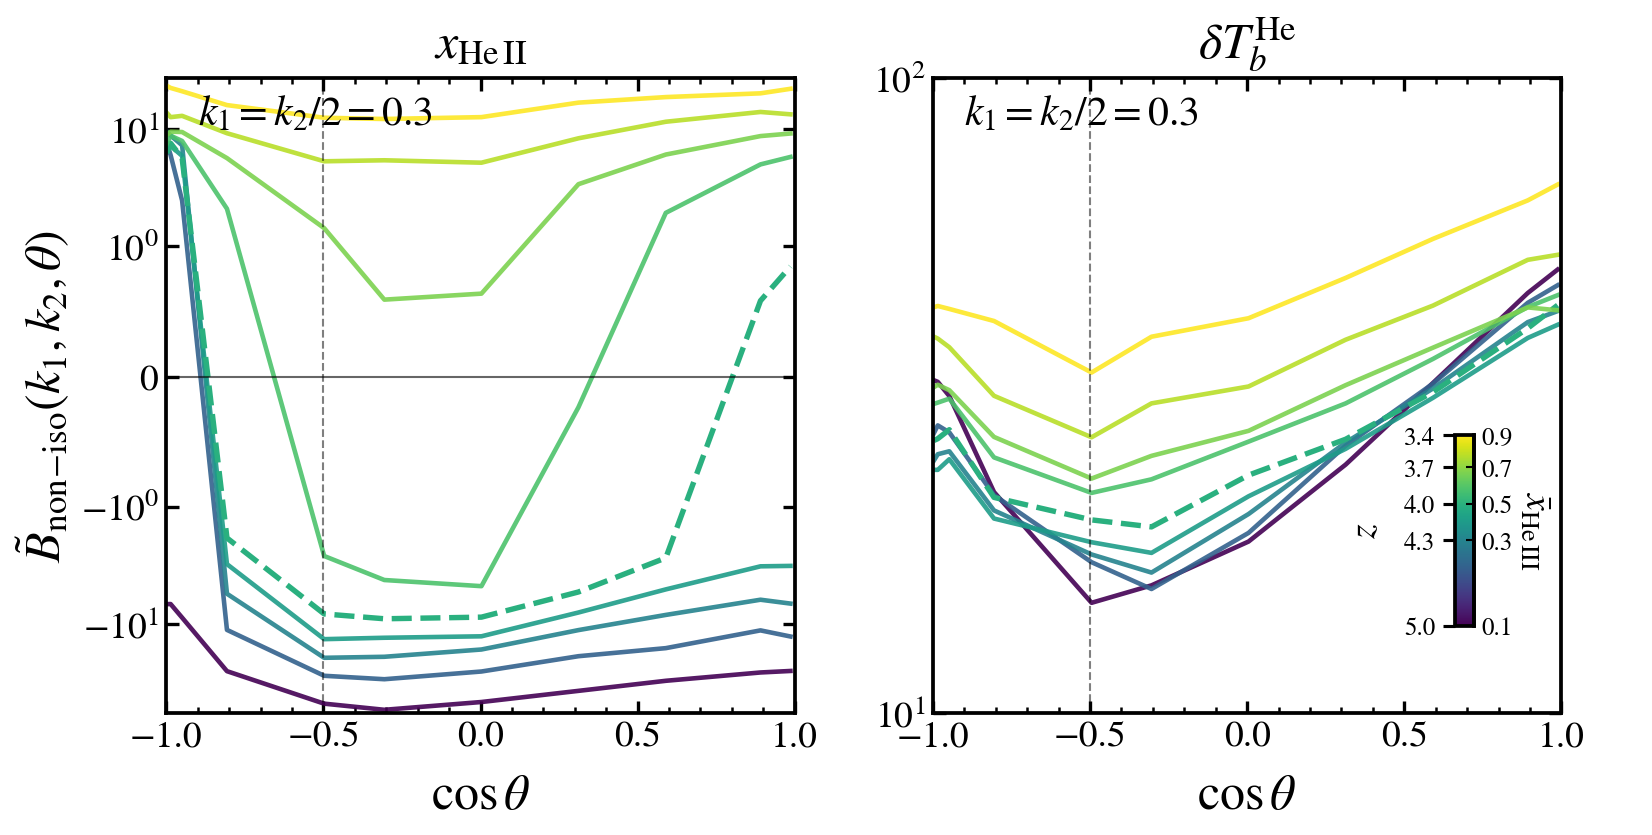
\includegraphics[width=\textwidth]{figs/non_iso_He.png}
    \caption{Redshift evolution of the non-isosceles bispectrum $\tilde{B}_\mathrm{non\text{-}iso}(k_1, k_2, k_3)$ for the singly ionized helium fraction $x_\mathrm{He\,II}$ (left panel) and the 3.46\,cm brightness temperature $\delta T_\mathrm{b}^\mathrm{He}$ (right panel), evaluated at the fixed configuration $k_1 = k_2/2 = 0.3\,h\,\mathrm{cMpc}^{-1}$. Colors and dashed curve follow the same convention as Figure \ref{fig:bispec_He_iso}. The right panel is displayed on a logarithmic scale, reflecting the entirely positive $\delta T_\mathrm{b}^\mathrm{He}$ bispectrum across all redshifts and configurations. The vertical dashed line marks the configuration at $\cos\theta = -0.5$.}
    \label{fig:non_iso_He}
\end{figure*}

To probe cross-scale mode coupling during helium reionization, we evaluate the non-isosceles configuration $k_1 = k_2/2 = 0.3\,h\,\mathrm{cMpc}^{-1}$. Retaining the same asymmetric triangle geometry as the hydrogen analysis bridges the characteristic scales of intermediate \ion{He}{3} bubble growth ($r_1 \approx 10\,h^{-1}\,\mathrm{cMpc}$) and late-stage \ion{He}{2} island fragmentation ($r_2 \approx 5\,h^{-1}\,\mathrm{cMpc}$). This direct comparison isolates how cross-scale interactions differ between stellar UV-driven hydrogen reionization and quasar-driven helium reionization.

%To probe cross-scale mode coupling in helium reionization, we now evaluate the non-isosceles configuration (the same used in the hydrogen analysis) defined by $k_1 = k_2/2 = 0.2\,h\,\mathrm{cMpc}^{-1}$, which simultaneously bridges the characteristic scales of intermediate \ion{He}{3} bubble growth ($r_1 \sim \pi/k_1 \approx 16\,h^{-1}\,\mathrm{cMpc}$) and late-stage \ion{He}{2} island fragmentation ($r_2 \sim \pi/k_2 \approx 8  h^{-1}\,\mathrm{cMpc}$) identified in the isosceles analysis. Using the same configuration for both epochs allows a direct comparison of cross-scale coupling between hydrogen and helium reionization, isolating the physical differences driven by stellar UV photons versus quasar radiation.


Figure \ref{fig:non_iso_He} shows the redshift evolution of the non-isosceles bispectrum for $x_\mathrm{He\,II}$ (left) and $\delta T_\mathrm{b}^\mathrm{He}$ (right). The $x_\mathrm{He\,II}$ field broadly mirrors the global topological inversion seen in hydrogen (Figure \ref{fig:non_iso_H}), transitioning from negative to positive as reionization completes. However, its collinear extremes exhibit distinct physics. The folded limit ($\cos\theta \to -1$) flips positive almost immediately after $z = 5$ ($\bar{x}_\mathrm{He\,III} = 0.1$). This rapid transition reflects the large-scale bias of quasar halos, which cluster small-scale \ion{He}{2} features around massive overdensities from the onset of reionization to imprint a positive cross-scale coupling signal. Toward the stretched limit ($\cos\theta \to 1$), the bispectrum turns strongly positive, capturing the sheet-like geometry of the \ion{He}{2} shells as the third leg probes scales below the characteristic \ion{He}{3} bubble radius. Together, these signatures confirm an inside-out helium reionization scenario where residual \ion{He}{2} clusters within large-scale environments shaped by quasar activity.



As in the hydrogen non-isosceles analysis, intermediate configurations display an asymmetric trough near $\cos\theta \approx -0.5$. Broken leg symmetry ($k_1 \neq k_2$) shifts this minimum, coupling the unequal base scales $r_1 \approx 10\,h^{-1}\,\mathrm{cMpc}$ and $r_2 \approx 5\,h^{-1}\,\mathrm{cMpc}$. While fixed in location by the triangle geometry, the trough amplitude evolves with redshift: early \ion{He}{3} voids deepen the negative signal, whereas late-time shell geometry and density contributions lift the trough toward positive values while maintaining it as the local minimum.


Comparing $x_\mathrm{He\,II}$ and $\delta T_\mathrm{b}^\mathrm{He}$ highlights a key distinction from the hydrogen non-isosceles case. Unlike $\delta T_\mathrm{b}^\mathrm{H}$ non-isosceles bispectrum, which remains negative over broad angular and redshift ranges, the  $\delta T_\mathrm{b}^\mathrm{He}$ non-isosceles bispectrum is positive across all configurations and redshifts. Two mechanisms drive this ubiquitous positivity. First, matter density coupling through $\delta T_\mathrm{b}^\mathrm{He} \propto x_\mathrm{He\,II}(1+\delta_\mathrm{b})(1 - T_\gamma/T_\mathrm{S}^\mathrm{He})$ imprints positive matter clustering onto the signal. Second, because $T_\mathrm{S}^\mathrm{He} \approx T_\gamma$ over most of the IGM, the thermal factor vanishes everywhere except near luminous quasars. This restricts the 3.46\,cm signal to rare, strongly overdense environments, rendering the bispectrum positive by construction. While both mechanisms contribute, this thermal selection is expected to dominate given the pervasive volume suppression of unheated regions.

%Comparing the $x_\mathrm{He\,II}$ bispectrum with the $\delta T_b^\mathrm{He}$ bispectrum reveals the deviation from the hydrogen non-isosceles case. As in the isosceles case, and unlike the hydrogen $\delta T_b^\mathrm{H}$ bispectrum that stays negative over a wide range of shapes and redshifts, the $\delta T_b^\mathrm{He}$ non-isosceles bispectrum is positive across all angular configurations and redshifts. Two effects drive this positivity, both absent or weaker in hydrogen. First, as in the hydrogen brightness-temperature case, the $(1+\delta_b)$ weighting in $\delta T_b^\mathrm{He} \propto x_\mathrm{He\,II}(1+\delta_b)(1 - T_\gamma/T_S^\mathrm{He})$ imprints the positive matter bispectrum onto the signal at high $k$. Second, and specific to helium, the thermal factor $(1 - T_\gamma/T_S^\mathrm{He})$ vanishes except near active sources, confining the signal to the rare, strongly clustered gas around AGN and star-forming regions; a signal restricted to such biased peaks is positive by construction. We expect the thermal selection to dominate, since $T_S^\mathrm{He} \approx T_\gamma$ over most of the volume, but do not separate the two contributions here.

%Comparing the $x_\mathrm{He\,II}$ bispectrum with the $\delta T_b^\mathrm{He}$ bispectrum reveals the deviation from the hydrogen non-isosceles case. As in the isosceles case, and unlike the hydrogen $\delta T_b^\mathrm{H}$ bispectrum that stays negative over a wide range of shapes and redshifts, the $\delta T_b^\mathrm{He}$ non-isosceles bispectrum is positive across all angular configurations and redshifts. The primary cause is the same: the matter bispectrum is strongly positive on these scales through non-linear gravitational collapse, and the $(1+\delta_b)$ weighting in $\delta T_b^\mathrm{He} \propto x_\mathrm{He\,II}(1+\delta_b)(1 - T_\gamma/T_S^\mathrm{He})$ imprints that positivity on the signal, increasingly outweighing the ionization term at high $k$.


%The \ion{He}{2} morphology reinforces this positivity. Rather than forming simple holes, $x_\mathrm{He\,II}$ concentrates in the ionization fronts bounding the \ion{He}{3} bubbles. The large-scale bias of the quasar hosts further amplifies this shell contribution wherever the fronts still lie in overdense gas, an effect strongest at early times when the bubbles are small. Together, these drive $\delta T_b^\mathrm{He}$ positive at all scales and epochs, in contrast to the partial cancellation seen for hydrogen.




%The sign evolution of the $x_\mathrm{He\,II}$ bispectrum toward the stretched limit directly reflects the growth of \ion{He}{3} bubbles. At high redshift, \ion{He}{3} bubbles are small and the triangle template is large enough to capture them as coherent below-average concentrations in the \ion{He}{2} field, driving the bispectrum negative. As reionization progresses and bubbles grow, the template increasingly probes the singly ionized helium gas between bubble boundaries rather than the bubble interiors themselves, driving the bispectrum toward positive values at lower redshift.


%The $x_\mathrm{He\,II}$ bispectrum thus remains the cleaner probe of helium ionization topology. The $\delta T_b^\mathrm{He}$ bispectrum, by contrast, encodes the interplay of \ion{He}{2} shell geometry, quasar large-scale bias, and the underlying density field, together providing a physically rich and complementary view of helium reionization.

%Finally, Figure \ref{fig:non_iso_He} presents the non-isosceles bispectrum for helium reionization, utilizing the specific configuration $k_1 = 0.4 \,\mathrm{cMpc}^{-1}$ and $k_2 = 0.8 \,\mathrm{cMpc}^{-1}$ to probe the cross-scale coupling between intermediate quasar-driven \ion{He}{3} regions and small-scale \ion{He}{2} fragments. Similar to the hydrogen epoch, the most prominent topological signatures emerge at the collinear extremes. As helium reionization progresses past its midpoint ($z \lesssim 4.2$), the signal at the folded limit ($\cos\theta \to -1$, where $k_3 \to 0.4 \,\mathrm{cMpc}^{-1}$) arcs sharply upward toward positive values. This enhancement mathematically isolates the presence of 1D filamentary structures, indicating that the residual \ion{He}{2} gas is continually compressed into narrow, interconnecting bridges as the massive \ion{He}{3} bubbles percolate. Concurrently, the stretched limit ($\cos\theta \to 1$, where $k_3 \to 1.2 \,\mathrm{cMpc}^{-1}$) displays a steep positive rise, confirming that these highly fragmented \ion{He}{2} islands remain deeply embedded within the 2D planar sheets that delineate the underdense cosmic voids.

%Furthermore, analyzing the intermediate triangle configurations reveals a clear breakdown of spherical symmetry in these cross-scale interactions. Unlike the isosceles helium bispectrum, which features a symmetric global minimum precisely at the equilateral configuration ($\cos\theta = -0.5$), the non-isosceles trough is noticeably asymmetric and shifted toward less negative values of $\cos\theta$. This distorted minimum confirms that while the dominant \ion{He}{3} regions may expand as quasi-spherical bubbles locally, their physical interplay with the small-scale \ion{He}{2} structures is fundamentally anisotropic, driven by the irregular distribution of the quasar sources.

%Finally, a comparison between the intrinsic $x_{\mathrm{He~II}}$ fraction (left panel) and the observable brightness temperature (right panel) underscores the powerful modulating effect of the underlying dark matter density. Within the $T^{\mathrm{He}}_b$ bispectrum, the negative trough is substantially deepened, and the positive gradients at both the folded and stretched extremes are severely steepened. As the observable signal is fundamentally density-weighted ($T^{\mathrm{He}}_b \propto x_{\mathrm{He~II}}(1+\delta_b)$), this amplification rigorously demonstrates that the final, highly anisotropic remnants of \ion{He}{2} are strictly coupled to the underlying density skeleton. Ultimately, the non-isosceles $T^{\mathrm{He}}_b$ bispectrum captures the complex, multi-scale reality of helium reionization, where quasar-driven astrophysics and the large-scale cosmic web inextricably intertwine.

\subsection{Bubble size evolution} \label{sec:bubble}

The characteristic size and topology of ionized regions encode source clustering, radiative feedback efficiency, and the inside-out progression of reionization. While \ion{H}{2} bubble sizes reflect stellar activity during hydrogen reionization, \ion{He}{3} bubble sizes encode the clustering and spectral hardness of quasars. Together, they trace two distinct IGM transformations driven by fundamentally different ionizing populations.



%The characteristic size and topology of ionized regions encode the clustering of ionizing sources, the efficiency of radiative feedback, and the inside-out progression of reionization, making them among the most physically informative diagnostics of the EoR. The size distribution of \ion{H}{2} regions at any given epoch reflects the integrated history of source activity and IGM topology, while the analogous \ion{He}{3} bubble sizes encode the clustering and spectral hardness of the quasar population driving helium reionization. Together, they provide complementary windows into two distinct epochs of IGM transformation driven by fundamentally different source populations.

Traditional geometric methods, such as the mean free path (MFP) \citep{Mesinger2007, Neyer2024} and friends-of-friends algorithms \citep{Iliev2006}, extract bubble sizes directly from 3D real-space ionization maps \citep[][]{Giri2018}. However, observational data from radio interferometers like HERA and the SKA are accessible only through Fourier-space summary statistics due to foreground contamination, noise, and instrumental limitations. This fundamental disconnect between real-space theoretical metrics and Fourier-space observational realities motivates developing methods that extract characteristic bubble sizes directly from Fourier-space statistical measures.
%Despite their physical importance, bubble sizes cannot be measured by current and near-future radio interferometers such as HERA and the SKA, as observations are inherently limited to Fourier-space statistics and are further complicated by significant foreground contamination and instrumental noise. More fundamentally, the ionization field is highly non-Gaussian and spans a wide, continuous distribution of bubble sizes simultaneously, meaning that no single characteristic scale dominates and standard one- and two-point statistics cannot capture the full morphological complexity of the topology. As a result, no single indirect method has yet emerged as a definitive probe of the bubble size distribution.


%Several approaches have been developed to characterize bubble sizes indirectly \citep[][]{Giri2018}. Geometric methods such as the mean free path (MFP) \citep{Mesinger2007, Neyer2024} and friends-of-friends algorithms \citep{Iliev2006} have been widely applied to simulated ionization fields, providing estimates of the characteristic bubble size and its evolution throughout reionization. However, these methods operate on real-space ionization maps and therefore cannot be straightforwardly applied to observational data, which is accessible only through Fourier-space statistics. This fundamental disconnect between theoretical characterization and observational accessibility motivates the development of methods that extract bubble size information from observable statistical quantities.


To bridge this gap, we pursue two Fourier-space statistical approaches to estimate bubble sizes directly from summary statistics. From two-point statistics, the peak of the ionized fraction power spectrum yields $R_\mathrm{ion} \sim 2.5/k_\mathrm{peak}$ \citep[e.g.,][]{Zaldarriaga2004, Furlanetto2004b}. From three-point statistics, the isosceles bispectrum sign flip provides a geometric estimate $R_\mathrm{ion} \sim \pi/k_{3,t}$ \citep[e.g.,][]{Majumdar2018, Hutter2020a}, where $k_{3,t} = k\sqrt{2(1+\cos\theta_t)}$ is the third side length at the zero-crossing angle $\theta_t$. Combining these 2-point and 3-point measures across hydrogen and helium reionization provides a complete mapping of bubble growth. Throughout this section, bubble size denotes the characteristic ionized radius ($R_\mathrm{ion}$), reported in $\mathrm{cMpc}$ to facilitate direct comparison with MFP estimates.

% For uncorrelated spherical ionized regions of radius $R$ \citep{Furlanetto2004b}, the one-bubble term of the ionized-fraction power spectrum is proportional to $V^2 W^2(kR)$, where $V$ is the bubble volume and $W(x) = 3(\sin x - x\cos x)/x^3$ is the Fourier transform of a spherical top-hat. The dimensionless power spectrum $\Delta^2 \propto (kR)^3 W^2(kR)$ then peaks at $kR \approx 2.46$, consistent with the feature at $k \sim 2/R$ identified by \citet{Zaldarriaga2004}. We therefore adopt $R_\mathrm{ion} \approx 2.5/k_\mathrm{peak}$. Because the power spectrum is weighted towards the largest ionized regions, this estimate traces the upper end of the bubble size distribution.
% This is the derivation. Both Zaldarriaga (Gaussian) and Mirocha (Spherical top-hat), the scale is around 2.5/k_peak, not 2\pi/k_peak.(Also derived it by myself) The review paper is mistaken. Fix the figure, and now I can mention why it was weird. Also, the reason why it doesn't match at higher ion fraction (or lower redshift) is the spherical shape assumption is not valid anymore.



\begin{figure*}[!t]
    \centering
    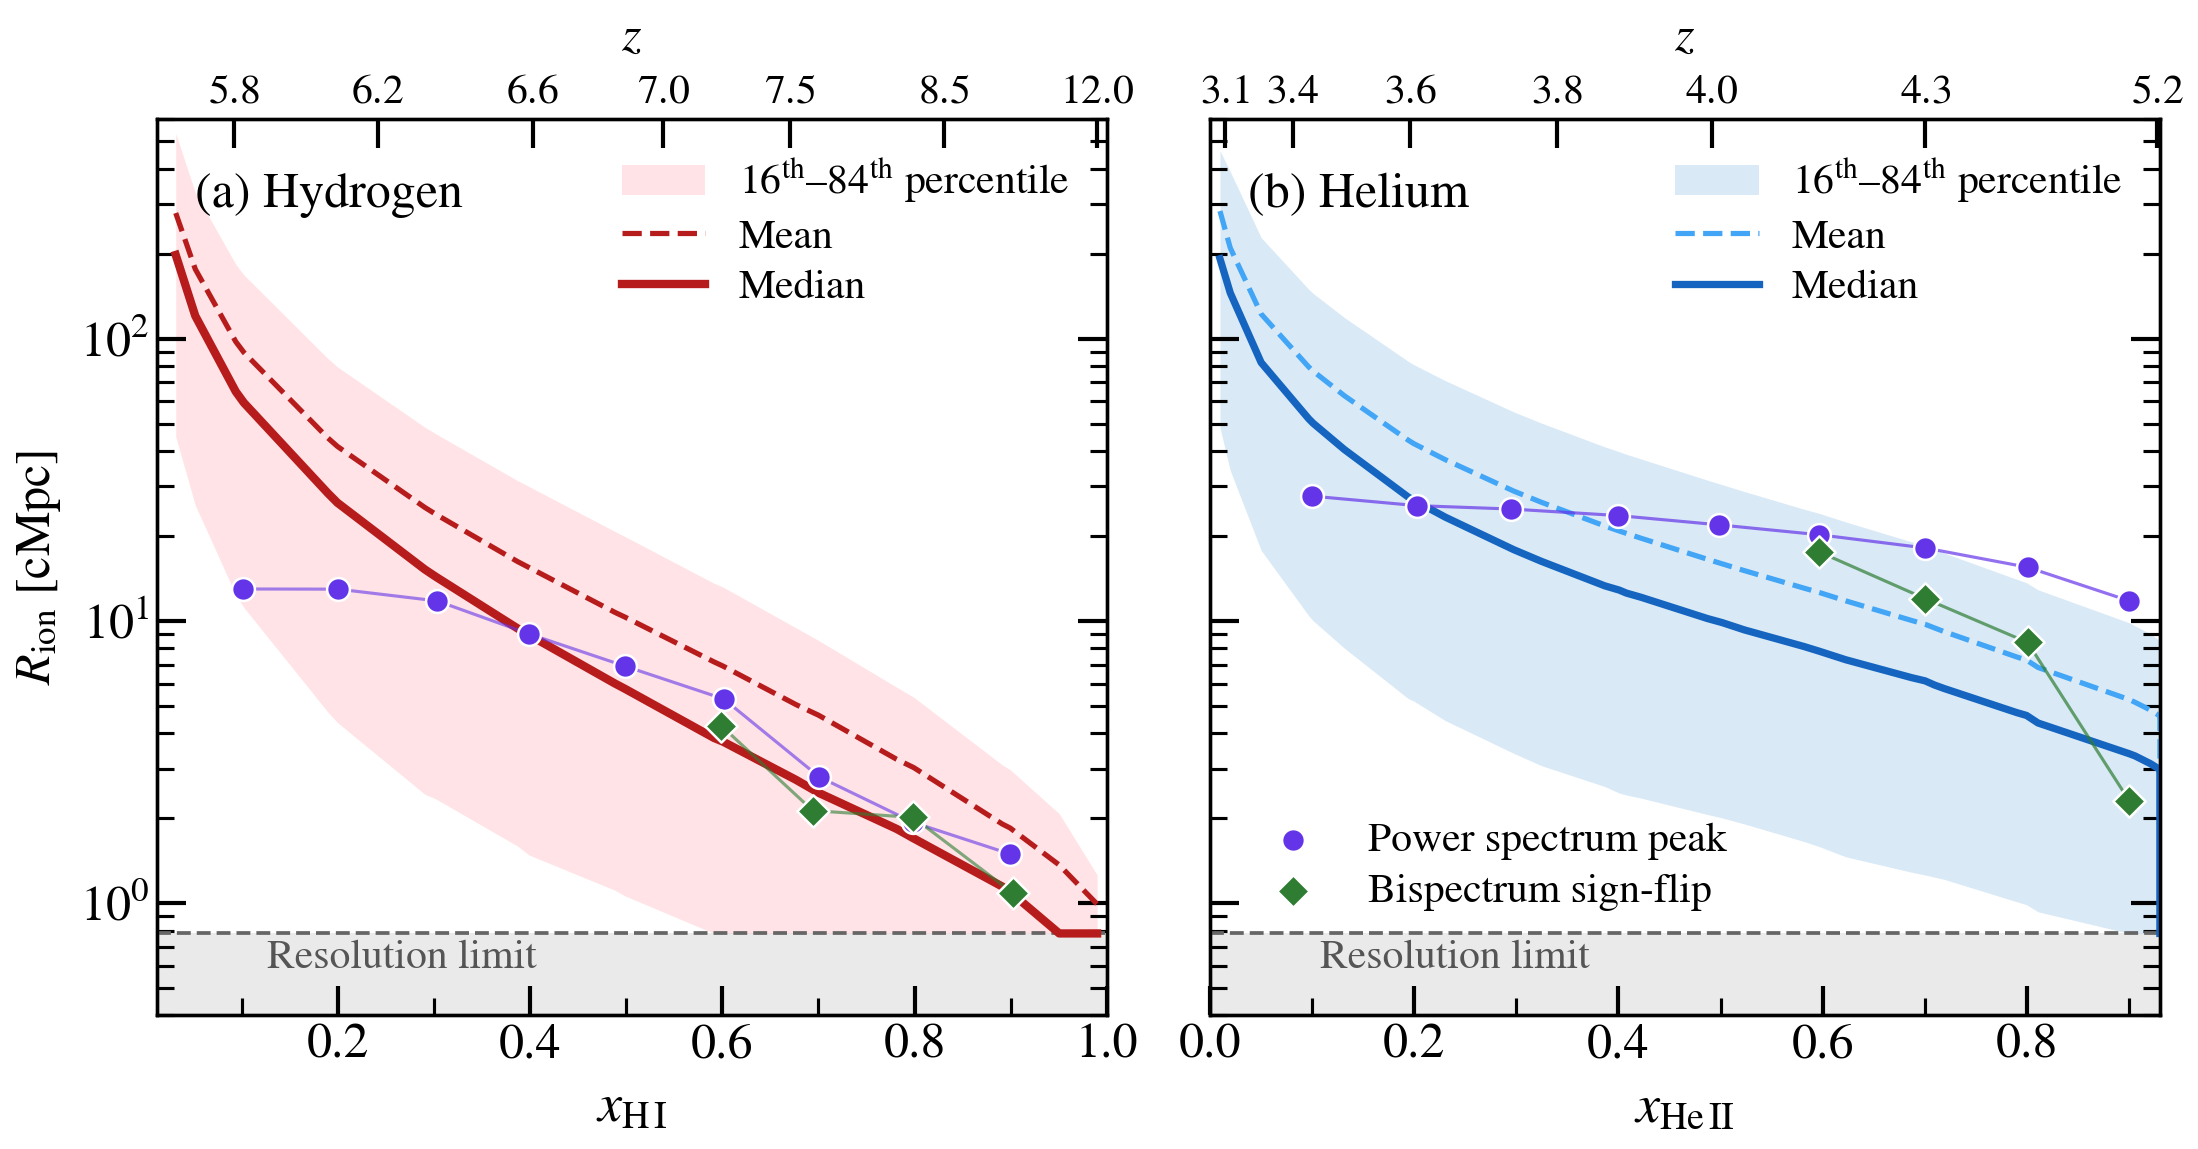
\includegraphics[width=\textwidth]{figs/BSD.png}
    \caption{Redshift evolution of the characteristic ionized bubble size during hydrogen reionization (panel a, $z \approx 5.8$--$12$) and helium reionization (panel b, $z \approx 3.1$--$5.2$). Shaded regions show the 16--84 percentile range, with the median (solid), and mean (dashed) overlaid; estimates from the power spectrum peak (circles) and bispectrum sign-flip (diamonds) are shown for comparison. The gray dashed line marks the resolution limit.}
    \label{fig:bubble_size}
\end{figure*}


\subsubsection{Hydrogen bubble statistics}

Figure \ref{fig:bubble_size} (a) presents the redshift evolution of the characteristic \ion{H}{2} bubble size from $z \approx 5.8$ to $z \approx 12$, derived using the MFP method of \citet{Neyer2024, Neyer2026}. Ionized cells are identified with a threshold $x_\mathrm{H\,II} > 0.5$, and rays are cast along 192 HEALPix directions from every ionized cell, with sub-cell interpolation of their end points \citep{Neyer2024}. The shaded region denotes the 16--84 percentile range of the bubble size distribution, illustrating the broad range of ionized structures coexisting at each epoch. The solid and dashed red curves show the median and  mean bubble sizes. The persistent offset between the mean and median demonstrates that a small number of large, merged ionized regions dominate the bubble size distribution throughout reionization, pulling the mean systematically above the median. Overlaid are independent bubble scale estimates derived from the power spectrum peak (purple circles) and the bispectrum sign-flip method (green diamonds), enabling direct comparison between real-space and Fourier-space estimators.

The median MFP radius grows monotonically from $\approx 1$\,cMpc at $z \approx 9.2$ to $\approx 65$\,cMpc at $z \approx 5.8$, with the mean $\approx 1.5$--$2$ times larger throughout. At the earliest epochs these values are limited by resolution, since $\approx 40\%$ of MFP rays at $z \approx 9.2$ end within a single $0.78$\,cMpc cell, and near the completion of reionization the rays trace the percolated ionized network rather than individual bubbles. This evolution reflects the progressive expansion and merger of ionized regions in an inside-out reionization scenario. Simultaneously, the broad percentile range demonstrates that reionization remains highly inhomogeneous, with small and large ionized structures coexisting across all stages of the EoR.


The power spectrum peak estimates follow the MFP scales, lying between the median and mean, at higher redshifts ($x_\mathrm{H\,I} \gtrsim 0.4$, $z \gtrsim 6.6$), but deviate from them at lower redshifts. In this regime, the power spectrum peak provides a reliable measure of the characteristic bubble radius. Below $x_\mathrm{H\,I} \approx 0.4$ ($z \lesssim 6.6$), however, the power spectrum estimate saturates at $\approx 13$\,cMpc, while the MFP sizes continue to grow. This flattening marks the percolation transition. Individual ionized bubbles lose their distinct identities and merge into a connected ionized network spanning a large fraction of the IGM. Beyond this point, $k_\mathrm{peak}$ no longer measures a bubble radius but most likely reflects the characteristic spacing of the connected ionized network and the remaining neutral islands.


The bispectrum sign-flip estimates track the median MFP scale more closely over the redshift range where the method is applicable. This closer agreement arises because the sign-flip method provides a more direct geometric probe of the characteristic transition scale between ionized bubble interiors and surrounding neutral gas. Consequently, it is less sensitive to the rarest, largest structures and instead traces the typical bubble morphology more faithfully. However, the method ceases to provide a clean ionized bubble scale once the global ionized fraction exceeds $\bar{x}_{\mathrm{H \,II}} \gtrsim 0.5$. Beyond this point, the topology of the IGM inverts. Ionized regions become the dominant phase, while the remaining neutral gas survives only as isolated islands. The bispectrum sign-flip then begins tracing the shrinking neutral islands rather than the expanding ionized bubbles.



%To place the \lumina bubble size distribution in a broader context, we compare our characteristic ionized radii against an analytic prediction and two independent observations in Figure \ref{fig:bubble_size} (a). The orange curve shows the analytic relation between the characteristic bubble radius and $x_\mathrm{H\,I}$ from \citet{Furlanetto2005}, derived without accounting for the overlap of ionized regions. Our median $R_\mathrm{ion}$ broadly tracks this prediction across most of the reionization history, but falls below it at the higher neutral fractions ($x_\mathrm{H\,I}\gtrsim0.8$), where the predicted bubbles approach our spatial resolution limit (grey shaded region) and are therefore systematically suppressed in the simulation.


%We further compare against observational constraints derived from Ly$\alpha$ damping wings in high-redshift galaxy spectra obtained with \textit{JWST}. The yellow square and arrows denote the $1\sigma$ limits on $x_\mathrm{H\,I}$ and $R_\mathrm{ion}$ for the triply lensed galaxy MACS0647$-$JD at $z=10.17$ \citep{Hsiao2024}, which infer a highly neutral IGM ($x_\mathrm{H\,I}\gtrsim0.9$) surrounding a sub-Mpc ionized region; this constraint is fully consistent with our predicted distribution. The teal squares show the characteristic bubble sizes and neutral fractions inferred from Ly$\alpha$ damping-wing absorption in 27 bright galaxies at $z=7$--$12$ \citep{Umeda2024}, which lie systematically above our median relation, particularly toward the end of the EoR. This offset is plausibly attributable to their assumption of a homogeneous IGM, which can lead to an overestimation of the inferred neutral fractions; alternatively, \citet{Keating2024} have shown using the Sherwood--Relics simulations that the large bubbles inferred at $z\sim7$ are difficult to reproduce under inhomogeneous reionization, and that the same damping-wing signatures can instead be explained by smaller ionized bubbles combined with larger intrinsic Ly$\alpha$ emission from the host galaxies.

%Taken together, the agreement of our characteristic $R_\mathrm{ion}$ with both the \citet{Furlanetto2005} analytic relation and the MACS0647$-$JD constraint, across an order of magnitude in bubble radius, supports the physical fidelity of the \lumina ionization morphology, with the single discrepant dataset explicable by a known modelling assumption rather than a deficiency of the simulation.




\subsubsection{Helium bubble statistics}

Figure \ref{fig:bubble_size} (b) presents the MFP-derived \ion{He}{3} bubble size evolution from $z \approx 5.2$ to $z \approx 3.1$. As in the hydrogen analysis, a persistent offset between the mean and median (blue solid and dashed curves) highlights a skewed distribution dominated by rare, large quasar-driven regions. Overlaid Fourier-space estimates from the power spectrum peak (purple circles) and bispectrum sign flip (green diamonds) enable direct comparison with these real-space metrics.

%The redshift evolution of the characteristic \ion{He}{3} bubble size from $z \approx 3.1$ to $z \approx 5.2$, derived using the MFP method is shown in Figure \ref{fig:bubble_size} (b). The shaded region denotes the 16--84 percentile range of the bubble size distribution, while the solid, dashed, and dotted green curves show the median, mean, and logarithmic mean bubble sizes, respectively. Similar to the hydrogen case, the persistent offset between the mean and median demonstrates that a small number of large quasar-driven ionized regions dominate the size distribution throughout helium reionization, pulling the mean systematically above the median. Overlaid are characteristic bubble scales independently inferred from the power spectrum peak (purple circles) and bispectrum sign-flip method (green diamonds), enabling direct comparison between real-space and Fourier-space estimators.


The MFP-derived bubble sizes grow steadily from $\sim 4$\,cMpc at $z \approx 5$ to $\sim 60$\,cMpc by $z \approx 3.4$. The broad percentile range highlights sustained spatial inhomogeneity, where small and extremely large \ion{He}{3} regions coexist as a direct consequence of the highly biased quasar population driving helium reionization.

% exhibit steady growth toward lower redshifts, with the characteristic \ion{He}{3} regions expanding from $\sim 4$\,cMpc at $z \approx 5$ to $\sim 50$\,cMpc by $z \approx 3.5$. Simultaneously, the broad percentile range demonstrates that helium reionization remains inhomogeneous throughout its evolution, with small and extremely large ionized regions coexisting across the IGM. This broad distribution reflects the highly biased nature of the quasar population responsible for driving helium reionization.

Unlike in hydrogen reionization, the helium power spectrum estimates exceed the MFP scales from the outset and grow far more slowly. They start at $\approx 12$\,cMpc at $x_\mathrm{He\,II} = 0.9$, about three times the MFP median, and grow only to $\approx 28$\,cMpc by $x_\mathrm{He\,II} = 0.1$, while the MFP median grows by an order of magnitude. Because quasars are rare and strongly clustered within massive overdensities, the \ion{He}{3} regions around neighbouring quasars overlap, so the two-point statistics likely trace the large-scale clustering envelopes of these quasar host environments, whereas the MFP measures the much smaller local distances to individual neutral boundaries. As in hydrogen, the power spectrum estimate then saturates while the MFP sizes keep growing, falling below the median for $x_\mathrm{He\,II} \lesssim 0.2$ as \ion{He}{3} regions percolate.

%In contrast to the hydrogen case, the power spectrum peak estimates remain systematically large across the entire redshift range, exhibiting only weak redshift evolution. This behavior indicates that the helium power spectrum is dominated almost immediately by the largest quasar-driven ionized structures. Because quasars are both rare and strongly clustered, the resulting \ion{He}{3} regions are highly biased and spatially extended even during the early stages of helium reionization. Consequently, the characteristic fluctuation scale extracted from the power spectrum preferentially traces these largest connected structures rather than the typical bubble size measured by the MFP distribution.

In contrast, bispectrum sign-flip estimates track the MFP-derived bubble scale far more closely than the power spectrum peak. Notably, the helium sign-flip scales lie closer to the MFP mean than the median. This shift occurs because helium reionization is driven by rare, highly luminous quasars, producing a heavily skewed bubble size distribution where the bispectrum 3-point topology is dictated by massive individual proximity zones, while the median MFP remains weighted by smaller local boundary distances. As in hydrogen reionization, this method reliably traces \ion{He}{3} bubbles during early stages ($x_\mathrm{He\,II} \gtrsim 0.6$, $z \gtrsim 4.2$), but ceases to yield a clean scale once percolation inverts the topology at lower $x_\mathrm{He\,II}$.


For comparable global ionized fractions, characteristic \ion{He}{3} bubble sizes are systematically larger than their \ion{H}{2} counterparts. This disparity stems from the distinct source populations driving the two epochs. While hydrogen reionization is powered by faint, highly abundant stellar sources, helium reionization is driven by rare, luminous quasars whose hard spectra and long photon mean free paths produce larger, more strongly clustered ionized regions. This structural distinction fades near reionization completion as individual bubbles percolate into box-scale networks.

%Notably, for comparable global ionized fractions, the characteristic \ion{He}{3} bubble sizes are systematically larger than their \ion{H}{2} counterparts. This reflects the fundamentally different source populations driving the two reionization epochs. Helium reionization is powered by rare, highly luminous quasars with hard ionizing spectra and long photon mean free paths, naturally producing larger and more strongly clustered ionized regions than the more numerous stellar sources responsible for hydrogen reionization. This distinction becomes less pronounced near the completion of reionization, where large ionized regions merge and the simulation volume approaches a fully ionized state.


Together, these estimators provide a complementary picture of ionization topology, where two-point power spectra trace large-scale spatial clustering, bispectrum zero-crossings isolate local bubble morphology, and MFP distributions map the underlying scale spectrum.


\section{Discussion}
\label{sec:discussion}

\subsection{Observational challenges: foregrounds and signal separation} \label{sec:foreground}



A primary challenge in detecting the 21\,cm and 3.46\,cm signals is the presence of astrophysical foregrounds that exceed the cosmological signal by up to four orders of magnitude \citep[][]{Dillon2014, Eastwood2019}. These foregrounds are intrinsically spectrally smooth, whereas the cosmological signal fluctuates rapidly in frequency. This separation enables two complementary strategies: (1) foreground avoidance, which restricts the analysis to the EoR window, and (2) foreground subtraction, which models and removes the contaminating emission directly. First-generation experiments, such as PAPER, MWA, and LOFAR, have applied these strategies to place increasingly stringent upper limits on the 21\,cm power spectrum, though current constraints remain $1$--$2$ orders of magnitude above predictions from simulations such as \lumina and \textsc{thesan-1}. Current and upcoming facilities, such as HERA \citep[][]{DeBoer2017} and the SKA \citep[][]{Koopmans2015, Chapman2015}, are designed to close this gap.


The 3.46\,cm hyperfine transition of $^3\mathrm{He\,II}$ offers a complementary but intrinsically fainter probe. Its faintness has two compounding causes. First, the low primordial abundance of $^3\mathrm{He}$ ($\sim 10^{-5}$ relative to hydrogen) sets a brightness temperature ceiling at the micro-Kelvin level; second, the weak coupling of the helium spin temperature to the gas suppresses it further, leaving the signal about five orders of magnitude below the 21\,cm signal \citep{Bagla2009, McQuinn2009}. While higher rest-frame frequency (8.67 GHz) benefits from reduced synchrotron emission and minimal ionospheric distortion, it is more susceptible to non-smooth contaminants such as low-redshift \ion{H}{1} emission, molecular transitions, and recombination lines, which cannot be removed by standard wedge-based techniques.


Given these challenges, direct auto-power spectrum detection of the cosmological helium signal remains out of reach for current and near-future interferometers such as SKA-1 MID and DSA-2000 \citep{Spina2025}. Forecasts indicate that the most viable near-term route for auto-spectrum measurements is a high-sensitivity single-dish survey, such as a PUMA-like facility \citep{Spina2025}. Cross-correlation presents a powerful complementary strategy by suppressing uncorrelated foregrounds and instrumental noise. The most natural cross-correlation target is the \ion{H}{1} 21\,cm signal itself: because $^3\mathrm{He\,II}$ emission originates within ionized hydrogen regions where neutral hydrogen has been destroyed, the 3.46\,cm and 21\,cm maps are intrinsically anti-correlated on small-to-intermediate scales, providing a distinct cosmological signature with independent systematic uncertainties \citep{Bagla2009, McQuinn2009, Takeuchi2014}.


Beyond the power spectrum detectability challenges discussed above, a related observational question concerns the one-point statistics. The VID statistics in Section~\ref{sec:vid} represent the intrinsic, real-space field and serve as a theoretical benchmark. Unlike visibility-based power spectrum estimators that bypass image reconstruction, measuring the VID requires map-space recovery, leaving it more vulnerable to instrumental effects and foreground contamination. Two primary mechanisms degrade these higher-order statistics. First, while additive Gaussian noise leaves raw cumulants untouched, its contribution to the total variance suppresses the normalized skewness and kurtosis. Second, resolution is strongly anisotropic, shaped by synthesized beam smoothing transversely and channel widths plus wedge-avoidance filtering along the line of sight. These combined effects can suppress intrinsic features or artificially induce non-zero kurtosis \citep{Kittiwisit2016}. Nevertheless, forward-modeled wedge-cut imaging demonstrates that HERA can recover the late-stage rise in 21\,cm skewness and kurtosis if window leakage is tightly controlled \citep{Kittiwisit2022}, while SKA1-Low granulometry shows topological bubble metrics remain recoverable down to $S/N \sim 3$ \citep{Kakiichi2017}. Precisely mapping these observational transfer functions requires a full instrument forward model of the \lumina lightcones, which we defer to future work.


% \citep{Ali2015, Jacobs2015}




\subsection{The necessity of large-scale volumes for \texorpdfstring{21\,cm and 3.46\,cm}{21 cm and 3.46 cm} convergence} \label{sec:box}


\begin{figure}[!t]
    \centering
    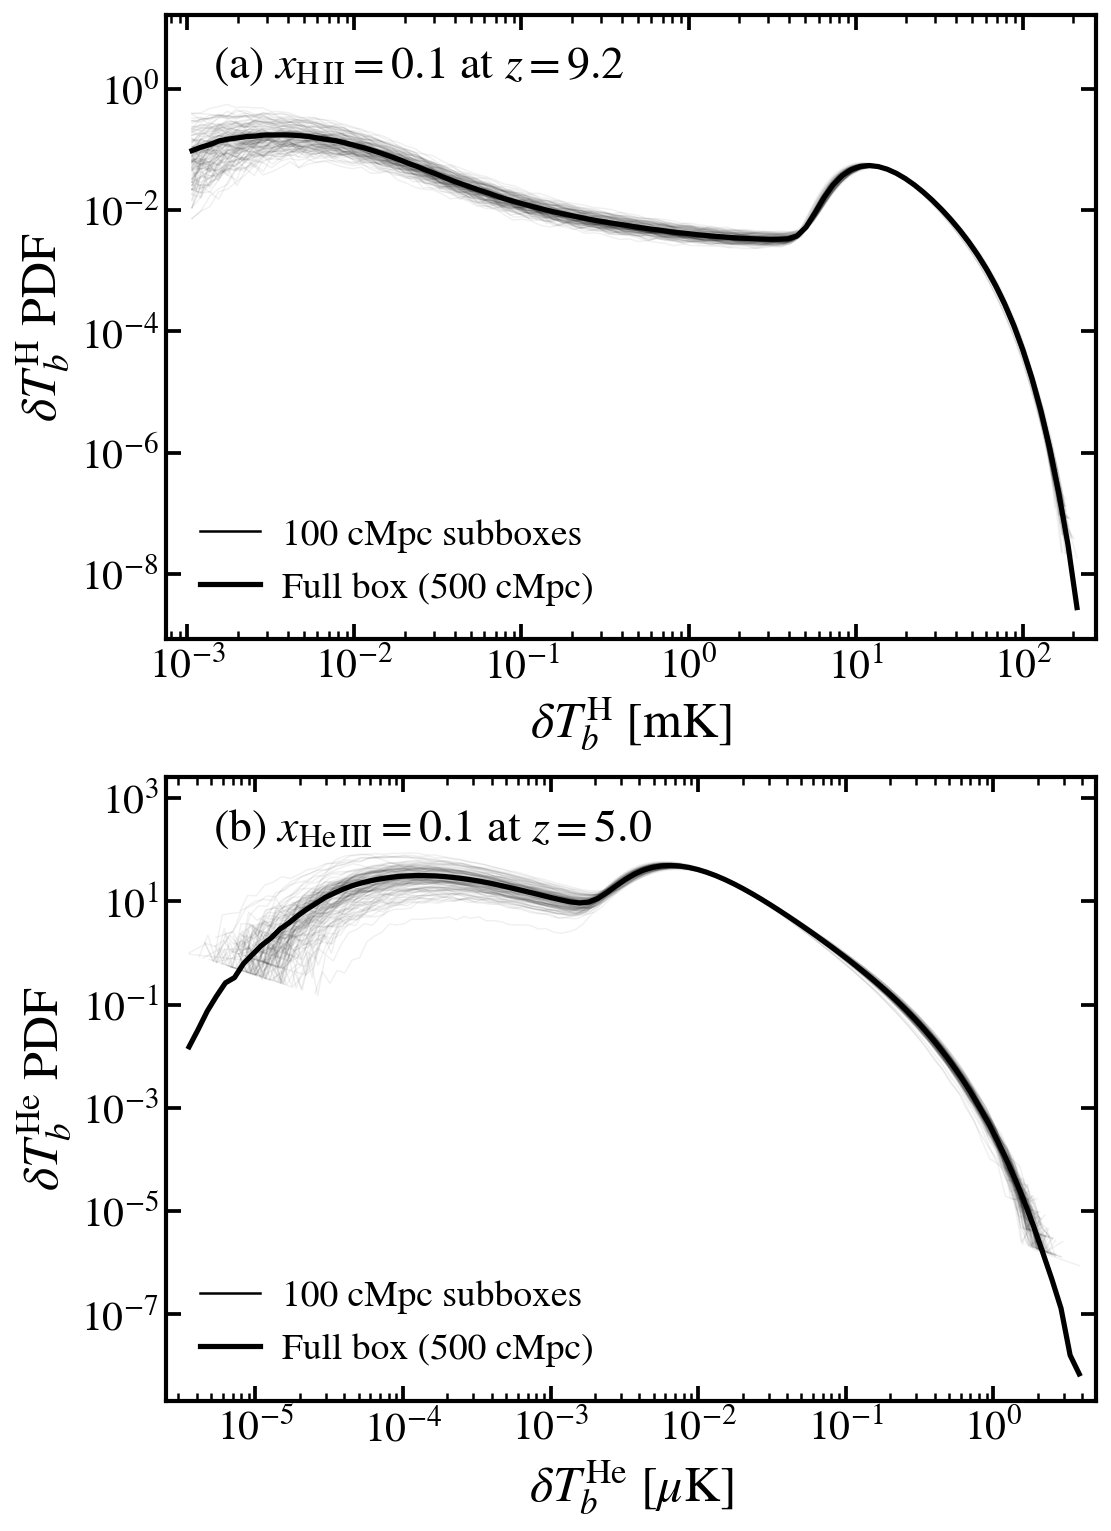
\includegraphics[width=\linewidth]{figs/subbox_VID.png}
    \caption{Cosmic variance of the brightness temperature probability distribution function (VID). Panel (a) shows the hydrogen 21\,cm VID at $z=9.2$ ($x_{\rm HII} = 0.1$), and panel (b) shows the helium 3.46\,cm VID at $z=5$ ($x_{\rm HeIII} = 0.1$). In both panels, the thick black line represents the converged distribution from the full 500\,cMpc \lumina\ volume, while the faint grey lines display the distributions extracted from 125 non-overlapping 100\,cMpc sub-volumes.}
    \label{fig:subbox}
\end{figure}

% Hydrogen
A critical consideration in 21\,cm cosmology is the simulation volume required to achieve statistical convergence. Previous studies have reported differing requirements. While \citet{Iliev2014} showed that box sizes of $\sim 100\,h^{-1}\,\mathrm{cMpc}$ are sufficient to capture the global reionization history, they argued that substantially larger volumes ($\gtrsim 200\,h^{-1}$\,cMpc) are required to converge the 21\,cm power spectrum, particularly at large scales ($k \lesssim 0.25\,h\,\mathrm{cMpc}^{-1}$) targeted by upcoming interferometers. In contrast, higher-resolution hydrodynamical simulations \citep{Gnedin2014a, Gnedin2014b, Kaurov2016} suggest that key statistics, including bubble size distributions and power spectrum amplitudes, may converge in significantly smaller volumes ($\sim 60$\,cMpc).


This apparent discrepancy reflects the distinct physical regimes probed by box size and spatial resolution. High-resolution simulations resolve Lyman-limit systems (LLSs) and dense filaments that act as photon sinks, constraining the local ionizing MFP and regulating small-scale bubble growth. However, spatial resolution alone cannot compensate for finite-volume effects. Large box sizes remain essential to suppress cosmic variance, sample the long-wavelength density modes, and capture the rare, highly biased sources that drive environment-dependent reionization histories ($z_\mathrm{reion}$). Consequently, while high resolution sets the local absorber-regulated boundary scales, large simulation volumes are necessary to accurately capture the full spatial scatter and large-scale ionization topology.

% Helium (mostly due to the quasar distribution)
The requirement for a large volume is even more stringent for helium reionization. Whereas hydrogen reionization is driven by abundant, weakly clustered star-forming galaxies, helium reionization is driven by quasars, which are orders of magnitude rarer and far more strongly clustered. Because quasars occupy the most massive, highly biased dark matter halos, the large-scale \ion{He}{3} field inherits severe sample variance: whether a specific sub-volume is quasar-rich or quasar-poor swings its  local reionization history far more strongly than for the galaxy population. Averaging down this variance to a representative mean requires spanning many quasar-clustering coherence lengths, which are among the longest in the Universe and cannot be captured in the $\sim 100\,\mathrm{cMpc}$ volumes typical of many hydrodynamical simulations. This demographic requirement is compounded by the radiation physics. The long mean free paths of hard ($>54.4$\,eV) photons produce characteristic \ion{He}{3} regions systematically larger than \ion{H}{2} regions at comparable ionized fraction (Section \ref{sec:bubble}), shifting the 3.46\,cm power spectrum toward lower wavenumbers where finite-box truncation is most severe. Consequently, the 500\,cMpc domain of \lumina is essential to properly sample the topology of helium reionization. This enhanced cosmic variance is directly reflected in the larger sub-volume scatter of the global helium signal relative to hydrogen (Figure \ref{fig:global}).

% The efforts to overcome this cosmic variance derived by the box size.

% Tada, so we introduce LUMINA!
By employing a 500\,cMpc volume, the \lumina simulation addresses both sides of this volume-resolution trade-off. It provides a sufficiently large domain to capture the largest ionized regions and long-wavelength modes relevant for HERA and SKA observations, while the adaptive resolution of the \textsc{arepo} moving mesh enables the tracking of dense absorbers that regulate the ionizing MFP. This combination reduces the sensitivity of the results to box-size effects present in smaller or lower-resolution simulations, and improves the robustness of the predicted 21\,cm and 3.46\,cm power spectra against artificial truncation of large-scale modes.


% To show the convergence, I choose the VID. For both H and He, we see the convergence. It also showes the lumina's strength to catch the large scale capturing ability in PS, of course for VID.


To demonstrate why our 500\,cMpc volume is necessary, we test how sensitive our simulated signals are to cosmic variance. Among our statistical measures, the one-point probability distribution function such as VID is particularly sensitive to box-size effects. Because the VID maps the complete distribution of the signal, small simulation volumes often fail to statistically sample rare, extreme environments. These under-sampled regions, such as the most massive early ionized bubbles or the hottest local areas, are exactly what populate the non-Gaussian tails of the distribution.


To quantify this, we divide the full \lumina volume into 125 non-overlapping 100\,cMpc sub-volumes and extract the 21\,cm VID. We perform this test at $z \approx 9.2$ (corresponding to $x_{\rm H\,II} \approx 0.1$), a transitional epoch where the global hydrogen spin temperature broadly exceeds the CMB temperature, yet local temperature and ionization fluctuations remain prominent before the signal is suppressed at later stages of reionization. As shown in Figure \ref{fig:subbox} (a), the full 500\,cMpc domain (thick black line) yields a smooth, well-sampled statistical distribution. The 100\,cMpc sub-volumes (faint lines) reproduce the bulk of the distribution but scatter substantially in the low- and high-$\delta T_b^\mathrm{H}$ tails. The bulk of the distribution converges because typical voxels are abundant even in a 100\,cMpc box. In contrast, the full volume is required to converge the rare structures in the tails, which carry the crucial non-Gaussian information probed by higher-order statistics.


Figure \ref{fig:subbox} (b) shows the corresponding VID for the helium 3.46\,cm signal at $z \approx 5$, chosen to match the $x_{\rm He\,III} \approx 0.1$ ionization fraction of the hydrogen case. At this epoch, the helium spin temperature exceeds the CMB temperature only marginally on average, approaching the gas kinetic temperature only locally, in the vicinity of quasars. This highly localized coupling, combined with the early patchwork of ionization, makes this transitional phase an ideal probe of cosmic variance. In the figure, the scatter among the 100\,cMpc sub-volumes is larger for helium than for hydrogen. This scatter is a direct consequence of the underlying source demographics: quasars are far rarer and more highly biased than star-forming galaxies, and their hard ionizing photons carve out systematically larger \ion{He}{3} regions. A 100\,cMpc volume fails to capture a representative sample of these massive, strongly clustered environments, whereas the 500\,cMpc \lumina volume successfully captures the converged statistical distribution, firmly justifying the necessity of the large-scale simulation domain.




\subsection{Theoretical uncertainties in the high-redshift universe} \label{sec:highz}


The first billion years of the Universe remain observationally elusive and therefore poorly constrained. In this regime, theoretical models play a central role in exploring a wide parameter space and identifying scenarios consistent with limited data. A major source of uncertainty lies in the properties of high-redshift sources, particularly the cosmic star formation rate density (SFRD). At early times, the SFRD is not directly constrained and is often assumed to follow the hierarchical growth of dark matter halos, rather than emerging from fully self-consistent baryonic physics.


Predicting the high-redshift SFRD is further complicated by computational limitations. Large-volume cosmological simulations are constrained by finite mass resolution, preventing them from resolving pristine minihalos ($T_\text{vir} < 10^4\,\mathrm{K}$), where star formation is initially driven by molecular hydrogen cooling. As a result, these simulations typically lack a self-consistent treatment of primordial stellar populations, particularly metal-free Population III (Pop III) stars. The properties of Pop III stars themselves remain highly uncertain. Early models assumed a top-heavy initial mass function (IMF) dominated by massive stars ($10$--$100\,\mathrm{M}_\odot$), while more recent simulations suggest fragmentation may produce lower-mass stars ($\sim 0.1$--$1\,\mathrm{M}_\odot$). This uncertainty is compounded by the potential role of miniquasars, the black hole remnants of massive Pop III stars whose long-mean-free-path X-rays can pre-heat the IGM \citep{Madau2004}. Together, these early source populations may produce radiation spectra and feedback processes that differ substantially from later generations. Consequently, the absence of these populations introduces significant uncertainty in modeling the early thermal and ionization history.


These theoretical uncertainties are compounded by the scarcity of direct observations at $z > 10$. In practice, models often rely on extrapolating locally calibrated relations to the early Universe. For example, the relation between star formation and X-ray luminosity ($L_X$--SFR), derived from nearby galaxies, may not hold under the low-metallicity and evolving compact object populations expected at high redshift.

Traditional observational probes provide limited constraints for resolving these degeneracies. Quasar sightlines exhibit saturated Gunn--Peterson absorption at $z \gtrsim 6$, restricting their usefulness to the final stages of reionization. Similarly, measurements of CMB polarization yield only an integrated optical depth ($\tau_e$), offering limited information on the timing and morphology of the process. While recent observations from \textit{JWST} suggest an unexpectedly high abundance of UV-luminous galaxies at $z > 10$ \citep[][]{Naidu2022, Harikane2023}, these surveys remain biased toward the brightest sources. As a result, they miss the faint populations that likely dominate reionization. In this context, the 21\,cm global signal and power spectrum provide a uniquely powerful probe of the aggregate emission from the full source population.


Given that the high-redshift SFRD remains poorly constrained, attempting to deterministically model a single reionization history is premature. In particular, star formation modeled under an effective equation of state is not fully predictive or converged at $z \gtrsim 10$, and high-redshift quasar populations carry substantial modeling uncertainties. Rather than claiming a definitive source prescription, \lumina provides an unprecedented large-volume RHD reference baseline for interpreting future observations. Next-generation facilities and upgraded current interferometers, including LOFAR and the SKA, are primarily sensitive to large-scale modes ($k \lesssim 0.1\,h\,\mathrm{cMpc}^{-1}$) and the global topology of ionized regions. By capturing these modes across a $500\,\mathrm{cMpc}$ domain while self-consistently tracking coupled radiation hydrodynamics, \lumina establishes a physically motivated benchmark to map uncertain source properties to observable 21\,cm and 3.46\,cm signatures.

%By prioritizing a large ($500\,\mathrm{cMpc}$) volume, \lumina captures these large-scale modes while maintaining sufficient resolution to model key physical processes. This approach enables systematic exploration of uncertain source parameters, mapping variations in the high-redshift SFRD to observable 21\,cm and 3.46\,cm signatures. As a result, the predicted ionization structures and power spectra provide physically motivated templates that can be directly tested against upcoming observational data.

%Because the true high-redshift SFRD remains fundamentally unconstrained, attempting to perfectly resolve the microphysics of a single, deterministic timeline is physically premature. Instead, macroscopic large-volume simulations like \lumina adopt a parametric, forward-modeling approach that is indispensable for interpreting future 21\,cm measurements. Next-generation interferometers, such as SKA and HERA, are predominantly sensitive to large-scale modes ($k \lesssim 0.1\,\mathrm{cMpc}^{-1}$) and the global topology of ionized and heated regions. By prioritizing a massive $500\,\mathrm{cMpc}$ volume, \lumina trades sub-grid parsec-scale detail for macro-scale statistical robustness. This framework allows us to systematically vary uncertain source efficiencies---mapping the disputed high-redshift SFRD to its corresponding large-scale 21\,cm signature. Ultimately, this strategy ensures that the predicted environmental dependencies, ionization structures, and resulting 21\,cm power spectra provide physically meaningful and rigorously testable templates, enabling observers to break theoretical degeneracies once the data arrives.




\subsection{Impact of X-ray heating efficiency and secondary ionizations} \label{sec:xray_heating}


A key physical limitation in the current \lumina implementation is the simplified treatment of X-ray energy deposition. At present, the simulation assumes that all absorbed X-ray energy is instantaneously converted into thermal heating (i.e., $f_{\rm heat} = 1$). In reality, the energy of a primary photoelectron is distributed among several channels: secondary ionizations of \ion{H}{1} and \ion{He}{1}, collisional excitations (which generate additional Lyman-$\alpha$ photons), and thermal heating through interactions with the ambient electron population \citep{Shull1985, Valdes2008}.


The heating efficiency, $f_{\rm heat}$, depends sensitively on the local ionization fraction, $x_e$, and evolves non-linearly throughout Cosmic Dawn. In the largely neutral IGM ($x_e \lesssim 10^{-4}$), only $\sim 10$--30\% of the deposited energy contributes to heating, with the remainder driving additional ionizations and excitations. These excitation channels are particularly important, as they enhance the Ly$\alpha$ background and can strengthen spin temperature coupling. As the ionization fraction increases, electron-electron interactions become more efficient, and a larger fraction of the energy is converted into heat.


By adopting $f_{\rm heat} = 1$, the fiducial \lumina run overestimates the IGM temperature during early Cosmic Dawn, consistent with \citet{Eide2020}, who showed that full heating efficiency overpredicts gas temperatures by up to a factor of $\sim 4$ at $z \approx 7.5$ compared with self-consistent energy partitioning. In the largely neutral early IGM, only $\sim 10$--$30\%$ of the absorbed X-ray energy is expected to heat the gas \citep{Shull1985, Furlanetto2010}. To illustrate the impact of this uncertainty, Figure~\ref{fig:global} (c) shows, alongside the fiducial signal and the post-processed adiabatic reference $\delta T^\mathrm{H}_{b,\mathrm{ad}}$, a linear interpolation between the two, $0.3\,\delta T_b^\mathrm{H} + 0.7\,\delta T_{b,\mathrm{ad}}^\mathrm{H}$ (labelled $f_\mathrm{heat} = 0.3$). Moving from the fiducial run towards the adiabatic reference, an absorption trough develops and the transition to net emission shifts to lower redshift. Because $\delta T_b$ is concave in $T_K$, this interpolation overstates the absorption expected from a self-consistent calculation at $f_\mathrm{heat} = 0.3$. Together with the approximate nature of the adiabatic reference, the curves therefore illustrate the direction and sensitivity of the effect rather than its precise amplitude.


\subsection{The cosmic timeline and milestone overlap} \label{sec:times}

The evolution of the 21\,cm signal is often described in terms of a sequence of key milestones defined by atomic physics and the emergence of radiation backgrounds. These include the collisional coupling era ($z \sim 30$--70), the onset of Cosmic Dawn ($z_\star \sim 30$), and the Ly$\alpha$ coupling transition ($z_\alpha$), when UV photons trigger the Wouthuysen--Field effect \citep{Wouthuysen1952, Field1958}. In practice, however, these milestones are neither sharply defined nor strictly sequential. Instead, they can overlap in both space and time, reflecting the coupled and inhomogeneous nature of early structure formation.


A key theoretical uncertainty lies in the relative timing of Ly$\alpha$ coupling ($z_\alpha$) and the heating transition ($z_h$), when X-ray radiation from early sources raises the IGM temperature above that of the CMB. Standard models typically predict $z_\alpha > z_h$ \citep[][]{Furlanetto2006, Mesinger2011, Pritchard2012, Mesinger2019}, leading to a prolonged absorption phase in the global 21\,cm signal. In \lumina, however, the efficient X-ray heating drives a near-simultaneous or slightly reversed ordering ($z_h \gtrsim z_\alpha$). As discussed in Section \ref{sec:xray_heating}, this enhanced energy deposition raises the IGM temperature above $T_\gamma$ before, or concurrently with, the full establishment of Ly$\alpha$ coupling.



As a result, the global 21\,cm signal in \lumina does not develop the deep absorption trough characteristic of standard models, transitioning rapidly into emission instead. We emphasize, however, that this outcome should be interpreted as a limiting case rather than a prediction. The fiducial run assumes maximal heating efficiency, $f_\mathrm{heat}=1$, in which all absorbed X-ray energy is deposited as heat. In reality, only a fraction of the secondary-electron energy heats the gas, with the remainder driving ionization and collisional excitation, so $f_\mathrm{heat}=1$ overestimates the heating and therefore the suppression of absorption. To investigate the opposite extreme, we also compute the adiabatic reference signal $\delta T_{b,\mathrm{ad}}^\mathrm{H}$ (blue dashed curve in Figure~\ref{fig:global} (c)), in which X-ray heating is removed from highly neutral gas; this recovers a canonical deep absorption trough near $z \approx 13$. The realistic signal therefore lies between these two limiting cases.



The relative timing of Ly$\alpha$ coupling and X-ray heating is bracketed in the same way. With $f_\mathrm{heat}=1$, the gas is heated above $T_\gamma$ before or as Ly$\alpha$ coupling is established ($z_h \gtrsim z_\alpha$), whereas an IGM without X-ray heating would remain colder than the CMB well after coupling ($z_\alpha > z_h$). Because a realistic $f_\mathrm{heat} < 1$ delays heating, we expect the canonical sequence $z_\alpha > z_h$ to hold, although rapid early heating remains plausible given the large uncertainties in the extreme-UV and X-ray output of early sources, including miniquasars and high-mass X-ray binaries \citep{Nusser2005}. These limiting cases illustrate how sensitively the global signal depends on the relative timing of the radiation backgrounds and on the still poorly constrained energy-deposition physics of early sources, which we examine in Section~\ref{sec:xray_heating}.

% \citep[][]{ShullvanSteenberg1985, FurlanettoStoever2010}
%

\begin{comment}


\subsection{The Impact of X-ray Heating: Exploring the Adiabatic Limit}


\begin{figure*}[!t]
    \centering
    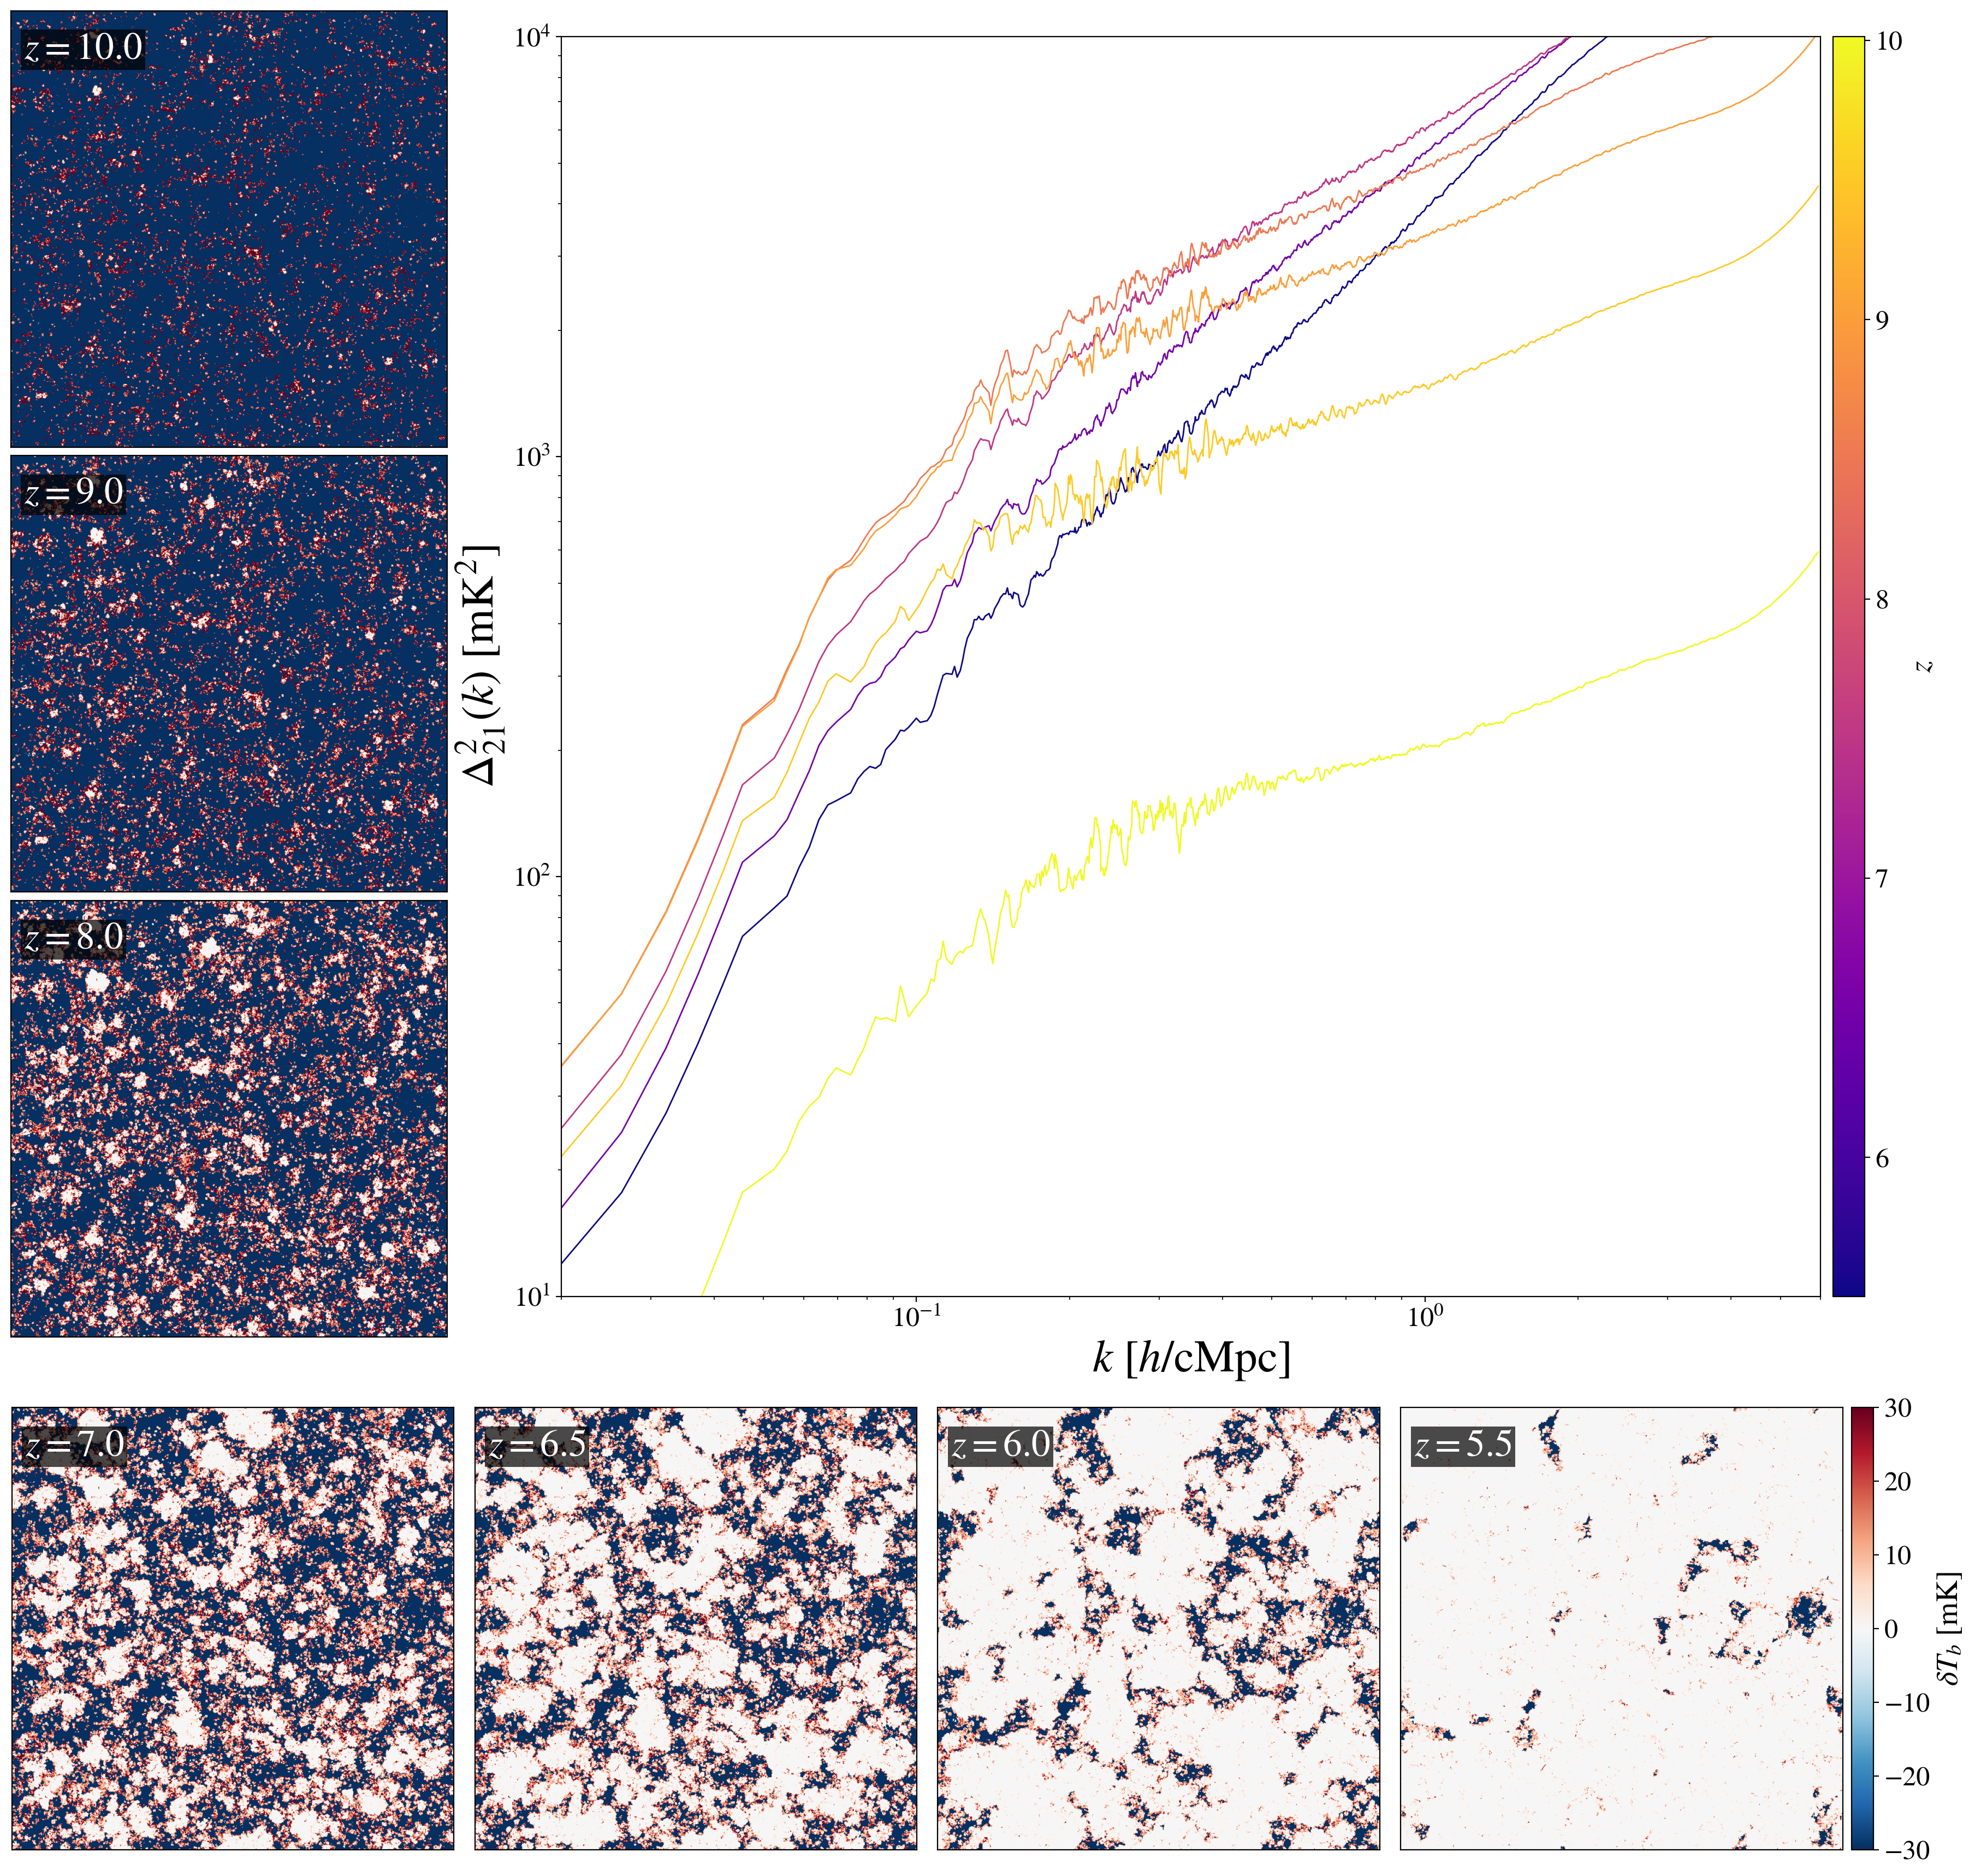
\includegraphics[width=\textwidth]{figs/adiabatic.png}
    \caption{21\,cm hydrogen temperature map but without the X-ray heating (adiabatic cooling)}
    \label{fig:adiabatic}
\end{figure*}


To isolate the role of X-ray heating on the 21\,cm morphology and statistics, we analyze a control run of \lumina wherein X-ray heating efficiency is explicitly set to zero. This scenario we assume that the IGM kinetic temperature evolves purely through adiabatic cooling driven by cosmic expansion, while the Wouthuysen-Field effect remains active via early stellar UV emission.

The resulting spatial and statistical evolution, presented in Figure \ref{fig:adiabatic}, is different from our fiducial model (See Fig. \ref{fig:ps_hydro}. In the absence of X-ray heating, $T_K$ rapidly drops well below the CMB temperature. Consequently, the neutral IGM outside of the expanding \ion{H}{2} bubbles is driven into deep absorption, visible as the prominent dark blue regions in the temperature maps. Rather than a gentle transition from absorption to emission, the morphology is characterized by an extreme thermal contrast between the freezing, deeply absorbing neutral background and the null signal ($\delta T^{H}_{b} = 0$\,mK) of the ionized bubbles.

This extreme spatial contrast radically alters the 21\,cm power spectrum. Because the power spectrum measures the spatial variance of the brightness temperature field, the massive contrast between the cold neutral gas and the ionized voids drives the amplitude of the fluctuations up by several orders of magnitude. As seen in the right upper panel of Figure \ref{fig:adiabatic}, the peak power reaches $10^3$--$10^4\,\text{mK}^2$, exceeding the fluctuations predicted by fiducial models with early X-ray heating by several orders of magnitude.

Crucially, this amplification makes the adiabatic limit highly testable. The overlaid thermal noise sensitivity curves for LOFAR, HERA, and SKA1-Low demonstrate that such an amplified signal would sit well above the noise thresholds of current and upcoming interferometers across a wide range of $k$-modes and redshifts (Need to check). The fact that current upper limits from instruments like LOFAR and HERA have not yet detected such a massive signal provides strong empirical evidence that some form of early IGM heating must have occurred prior to the midpoint of reionization.


\subsection{Modeling Tensions and the EDGES Anomaly}

Finally, there is a discrepancy between analytical models and numerical simulations regarding the global signal's morphology. Analytical frameworks often predict deep absorption troughs reaching $\sim -100$\,mK \citep{Pritchard2008}, whereas self-consistent simulations like \textsc{CROC} find much shallower features ($\sim -25$\,mK) due to more realistic background coupling \citep[][]{Gnedin2014a, Gnedin2014b, Kaurov2016}. This tension is further exacerbated by the \textit{EDGES} reported detection of a $-500$\,mK trough \citep{Bowman2018}, which exceeds standard $\Lambda$CDM limits and has prompted debates over exotic physics, such as dark matter-baryon scattering or an unexpected excess radio background \citep{Barkana2018, Fialkov2019}. \lumina could serve as a critical tool to explore these boundaries by providing the large-scale statistical context necessary to distinguish between these competing physical models.
\end{comment}


\section{Conclusion}
\label{sec:concl}

In this work, we present the first large-scale 21\,cm and 3.46\,cm observational predictions from the \lumina project, a $500\,\mathrm{cMpc}$ RHD simulation that couples galaxy and AGN growth to the thermal and ionization evolution of the IGM. Previous state-of-the-art RHD simulations, limited to volumes $\lesssim 100\,\mathrm{cMpc}$, are susceptible to cosmic variance and unable to capture the long-wavelength radiation modes necessary for accurate predictions. The $500\,\mathrm{cMpc}$ volume of \lumina overcomes this limitation, simultaneously resolving the dense environments driving hydrogen reionization and the rare, massive quasars responsible for helium reionization. Consequently, \lumina provides the community with robust theoretical benchmarks, largely free from severe finite-volume effects and specifically tailored to the large-scale modes ($k \lesssim 0.1\,h\,\mathrm{cMpc}^{-1}$) targeted by next-generation interferometers such as SKA and HERA.


Based on this framework, the principal findings of our study are summarized as follows:
\begin{itemize}
\item \textbf{Thermal and Ionization Timeline:} The global 21\,cm signal is highly sensitive to the relative timing of Ly$\alpha$ coupling ($z_\alpha$) and X-ray heating ($z_h$). In our fiducial maximal-heating model ($f_{\rm heat}=1$), efficient X-ray heating produces a near-simultaneous or reversed ordering ($z_h \gtrsim z_\alpha$), suppressing the canonical deep absorption trough and driving an early transition to emission. We caution that $f_{\rm heat}=1$ represents an upper limit on the heating efficiency; a self-consistent partition of the absorbed X-ray energy among heating, secondary ionization, and excitation (Section~\ref{sec:xray_heating}) would deepen the trough. Indeed, a post-processed adiabatic reference without X-ray heating recovers the standard absorption feature, demonstrating that the global signal morphology directly probes early X-ray efficiencies. Extending the simulation to $z=3$, \lumina further connects this early evolution to the later, AGN-driven epoch of helium reionization. We note that below $z=4.75$ the radiation field is reduced to a single AGN-dominated bin, with the \ion{H}{1}/\ion{He}{1} photoionization rates replaced by a spatially uniform UV background. This simplification is appropriate for the \ion{He}{2} reionization epoch that is the focus of our low-redshift analysis, and yields a continuous thermal history from Cosmic Dawn to a fully ionized Universe.

\item \textbf{Large-Scale Topology and Multi-Point Statistics:} Accurately capturing the morphology of reionization requires both large simulation volumes and higher-order statistics. Using the $500\,\mathrm{cMpc}$ \lumina volume, we analyze the ionization and brightness temperature fields through one-point VID, two-point (power spectrum), and three-point (bispectrum) statistics. The power spectrum alone cannot capture the non-Gaussian, binary topology of ionized regions, motivating the one- and three-point statistics that probe the asymmetry and phase structure of the fields. \lumina resolves the large-scale modes ($k \lesssim 0.1\,h\,\mathrm{cMpc}^{-1}$) relevant for SKA and HERA, while enabling a statistical characterization of helium reionization, which is driven by rare, luminous quasars and therefore requires large cosmological volumes.

\item \textbf{Bubble Size Evolution and Reionization Topology:} Using complementary real-space and Fourier-space estimators, we characterize the evolving ionization topology during both hydrogen and helium reionization. We find that the ionization topology remains strongly non-Gaussian throughout both epochs, as captured by the increasing skewness and kurtosis of the VID. The bubble size distribution has an extended large-scale tail, pushing the mean systematically above the median. For hydrogen, the power spectrum peak tracks the characteristic bubble radius before percolation and saturates once ionized regions merge, whereas for helium it traces the large-scale clustering of quasar-driven \ion{He}{3} regions. The bispectrum sign flip most closely follows the characteristic local bubble scale. At comparable ionized fractions, helium ionized regions are larger than hydrogen bubbles until the late stages of reionization, reflecting the rarer, harder, and longer MFP radiation of the quasar population driving helium reionization.

\item \textbf{Helium as a Complementary Probe:} The 3.46\,cm signal provides a distinct tracer of the later, quasar-driven phase of reionization. Unlike hydrogen, this signal is strongly localized to dense, quasar-illuminated structures, offering a complementary view of the IGM and the role of hard radiation sources.
\end{itemize}

%Several limitations define the scope of the present results. Because the simulation does not resolve pristine minihalos or Pop~III star formation, the absolute timing of the earliest Cosmic Dawn milestones carries significant uncertainty; we emphasize, however, that our reionization-era statistical results ($z\lesssim10$) are insensitive to this limitation, as they are dominated by resolved atomic-cooling halos and AGN.


%Looking ahead, the large volume and multiphase modeling of the \lumina suite provide a natural framework for multi-tracer studies of the high-redshift Universe. While facilities such as JWST are revealing the properties of luminous galaxies at $z > 10$, they do not directly probe the diffuse IGM that these sources heat and ionize. \lumina bridges this gap by linking galaxy populations to their large-scale IGM environment, enabling a consistent interpretation of observations across scales.

%Building on this, future work will extend the framework beyond the 21\,cm and 3.46\,cm signals to include Line Intensity Mapping (LIM) tracers such as CO and [\ion{C}{2}]. By cross-correlating these tracers with the 21\,cm field, we can connect the distribution of galaxies to the surrounding ionization and thermal structure of the IGM. Combined with the tracking of hydrogen and helium evolution, this multi-tracer approach offers a powerful pathway for constraining the physics of early star formation and black hole growth.


The results emphasized here are the ionization topology and large-scale statistics, for which the 500 cMpc volume of \lumina\ is essential. In the saturated EoR regime ($z \lesssim 10$), the hydrogen 21\,cm signal is additionally insensitive to the exact spin temperature, since $T_S^\mathrm{H} \gg T_\gamma$. We do not extend this insensitivity to the Cosmic Dawn 21\,cm signal or to the 3.46\,cm signal: both depend on the thermal and spin-coupling history and are therefore subject to the limitations discussed above. Conversely, reliable modeling of the thermal history and early spin-temperature coupling is precluded by the numerical approximations: the M1 closure, a reduced speed of light, the omission of cosmological redshifting during radiative transfer (which is particularly relevant for large box sizes), maximal X-ray heating ($f_\mathrm{heat}=1$), and unconverged global star formation rate density at $z \gtrsim 10$ (Section~\ref{sec:discussion}). Capturing this microphysics reliably may require complementary small-box simulations affording multi-frequency transport with self-consistent energy partitioning, full light-speed propagation \citep[e.g.,][]{Gnedin2026}, and a directly computed spin temperature, together with the higher resolution \citep[][]{Kannan2025} and Population III modeling \citep[e.g.][]{Saha2026} needed to converge the early star formation rate.


% Maybe this?
Future work could extend the \lumina framework to generate realistic lightcone simulations, capturing light-travel time evolution along the line of sight, and to include additional line intensity mapping tracers such as CO and [\ion{C}{2}]. Cross-correlating these tracers with the 21\,cm field will connect the galaxy distribution to the surrounding ionization and thermal structure of the IGM. Evaluating signal recovery will require combining these lightcones with comprehensive instrument forward-modeling, incorporating realistic primary beams, channel resolutions, foreground filtering, and thermal noise floors for specific survey configurations. Together with the joint tracking of hydrogen and helium reionization presented here, this multi-tracer lightcone pipeline provides a realistic platform for constraining early star formation and black hole growth.


\section*{Acknowledgments}

An award of computer time was provided by the INCITE program. This research used resources of the Oak Ridge Leadership Computing Facility at the Oak Ridge National Laboratory, which is supported by the Advanced Scientific Computing Research programs in the Office of Science of the U.S. Department of Energy under Contract No.\ DE-AC05-00OR22725. RK acknowledges support from the Natural Sciences and Engineering Research Council of Canada (NSERC) through a Discovery Grant and a Discovery Launch Supplement, funding reference numbers RGPIN-2024-06222 and DGECR-2024-00144, and from York University's Global Research Excellence Initiative. Support for programs JWST-AR-08709 (AS) and JWST-AR-04814 (XS, MV) were provided by NASA through a grant from the Space Telescope Science Institute, which is operated by the Association of Universities for Research in Astronomy, Inc., under NASA contract NAS 5-03127.
LH and VS acknowledge support from the Simons Foundation through the ``Learning the Universe'' initiative. MV acknowledges support through NASA ATP Grant 23-ATP23-149 and NSF AAG Grant AST-2307699. This work was supported by the LOEWE programme of the State of Hesse (LOEWE-Spitzen-Professur).


\bibliographystyle{mnras}

% You should give the same name for your .bbl as your main .tex
% since it is a requirement for posting on ArXiv.
\bibliography{oja_template}


\begin{appendix}
\section{Spin Temperature and the \texorpdfstring{Ly$\alpha$}{Lyman-alpha} Background}
\label{ap:calculation}


\begin{figure*}[!t]
    \centering
    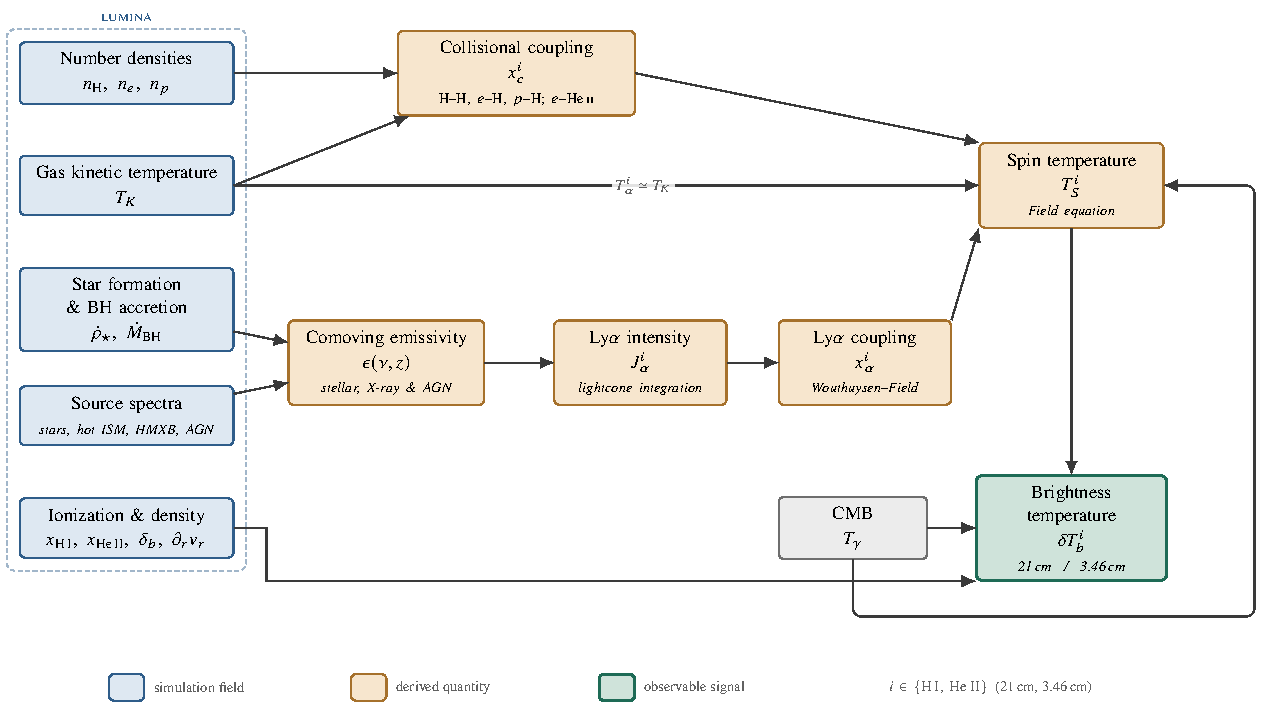
\includegraphics[width=\textwidth]{figs/flowchart.pdf}
    \caption{Data flow diagram converting \lumina grid fields (blue) into intermediate quantities (orange) and final brightness temperatures (green) for $i \in \{\mathrm{H\,I},\ \mathrm{He\,II}\}$.}
    \label{fig:flowchart}
\end{figure*}

In this Appendix, we provide the complete framework used to calculate the spatially resolved spin temperatures for both hydrogen and helium. These temperatures are governed by the balance of collisional and radiative processes. We first outline the calculation of the collisional and Ly$\alpha$ coupling coefficients. Because the Ly$\alpha$ coupling depends heavily on the local radiation field, we subsequently detail the lightcone integration used to compute the proper Ly$\alpha$ intensity, followed by the specific stellar and high-energy source emissivities that build this background in \lumina.

Figure~\ref{fig:flowchart} summarizes how the \lumina grid fields enter this calculation for both the 21\,cm and 3.46\,cm brightness temperatures. The local number densities and gas kinetic temperature $T_K$ set the collisional coupling $x_\mathrm{c}^i$ directly, while star formation rates, black hole accretion rates, and BPASS spectra determine the comoving emissivity $\epsilon(\nu, z)$ and the resulting Ly$\alpha$ intensity $J_\alpha^i$ and Wouthuysen--Field coupling coefficients $x_\alpha^i$. These two coupling coefficients, together with $T_K$ and the CMB temperature $T_\gamma$, yield the spin temperature $T_S^i$ via the Field equation (Equation~\ref{eq:Ts}); the differential brightness temperature then follows from Equations~(\ref{eq:21cm}) and~(\ref{eq:helium}) once the local ionization state and baryon overdensity are incorporated. Evaluated cell by cell, this calculation ensures that $T_S^i$ and $\delta T_b^i$ preserve the full spatial structure of the \lumina volume.

\subsection{Spin temperature}

The detectability of the 21\,cm and 3.46\,cm signals fundamentally depends on the spin temperatures of \ion{H}{1} and $^3$He\,II, $T_S^{\rm H}$ and $T_S^{\rm He}$. In each case, the spin temperature is determined by three competing physical processes: (1) the absorption and emission of resonant hyperfine photons coupling the gas to the radio background (primarily the CMB); (2) collisions with surrounding particles (neutral hydrogen atoms, free electrons, and protons in the case of \ion{H}{1}, and predominantly free electrons in the case of $^3$He\,II, which only exists in ionized regions); and (3) the resonant scattering of Ly$\alpha$ photons, which induces a spin-flip transition via an intermediate electronic excited state \citep[Wouthuysen--Field effect;][]{Wouthuysen1952, Field1958}. The relevant Ly$\alpha$ photons are \ion{H}{1} Ly$\alpha$ (10.2~eV) for hydrogen and \ion{He}{2} Ly$\alpha$ (40.8~eV) for helium.

Assuming the Rayleigh-Jeans limit, the equilibrium balance of these three processes yields the Field equation \citep{Furlanetto2006, McQuinn2009}, identical in functional form for both species:
\begin{equation}
    \left(T_S^i\right)^{-1} = \frac{T_\gamma^{-1} + x_\alpha^i
    \left(T_\alpha^i\right)^{-1} + x_c^i \, T_K^{-1}}
    { 1 + x_\alpha^i + x_c^i}\,,
    \label{eq:Ts}
\end{equation}
where $i \in \{{\rm H}, {\rm He}\}$ labels the species, $T_\alpha^i$ is the color temperature of the relevant Ly$\alpha$ radiation field at the corresponding resonance frequency (\ion{H}{1} Ly$\alpha$ for hydrogen, \ion{He}{2} Ly$\alpha$ for helium), $T_K$ is the gas kinetic temperature, and $x_c^i$ and $x_\alpha^i$ are the species-specific coupling coefficients due to atomic collisions and the scattering of Ly$\alpha$ photons, respectively.

Typically, the Ly$\alpha$ color temperature is tightly coupled to the gas kinetic temperature, $T_\alpha^i \approx T_K$, for both species. Because the IGM is optically thick to the relevant Ly$\alpha$ photons in regions where the corresponding ion is abundant---\ion{H}{1} Ly$\alpha$ throughout the bulk neutral IGM, and \ion{He}{2} Ly$\alpha$ within \ion{He}{2} regions during helium reionization---the enormous number of resonant scattering events thermalizes the radiation field, driving the Ly$\alpha$ spectral profile toward a blackbody distribution at temperature $T_K$ near the line center \citep{Wouthuysen1952}. This condition is readily fulfilled throughout the high-redshift IGM in our simulated cosmology.





\subsection{Coupling coefficients}

\subsubsection{Collisional coupling coefficients}


The collisional excitation and de-excitation of the \ion{H}{1} hyperfine levels dominate the spin temperature evolution in highly dense gas. Consequently, this coupling mechanism is the primary driver of the 21\,cm signal in the very early Universe (e.g., during the Dark Ages) when the mean cosmic gas density is exceptionally high. The overall collisional coupling is mediated by three primary interaction channels: (1) collisions between neutral hydrogen atoms (H-H), (2) hydrogen-electron collisions (H-e), and (3) hydrogen-proton collisions (H-p).

The total collisional coupling coefficient for hydrogen is

\begin{equation}
    \begin{split}
        x^\mathrm{H}_{c} & = x^\mathrm{HH}_c + x^\mathrm{eH}_c + x^\mathrm{pH}_c \\
        & = \frac{T^\mathrm{H}_{\star}}{A^{\mathrm{H}}_{10}T_\gamma} \left[ \kappa^\mathrm{HH}_{1-0} (T_K) \,n_H + \kappa^\mathrm{eH}_{1-0} (T_K) \,n_e + \kappa^\mathrm{pH}_{1-0} (T_K) \,n_p \right]\,,
    \end{split}
\end{equation}
where $T^\mathrm{H}_{\star} \equiv h\nu_{21\mathrm{cm}}/k_B \approx 0.068$ K is the temperature corresponding to the 21\,cm transition energy, $A^\mathrm{H}_{10} \approx 2.85 \times 10^{-15} \text{ s}^{-1}$ is the Einstein spontaneous emission coefficient for hydrogen, $n_H$, $n_e$, and $n_p$ are the local number densities of neutral hydrogen, free electrons, and protons, respectively, and $\kappa^\mathrm{HH}_{1-0}$, $\kappa^\mathrm{eH}_{1-0}$, and $\kappa^\mathrm{pH}_{1-0}$ are the specific $1 \to 0$ hyperfine de-excitation rate coefficients for collisions with other neutral hydrogen atoms \citep{Allison1969}, free electrons \citep{Furlanetto2007eH}, and protons \citep{Furlanetto2007pH}.


For the singly ionized helium signal, the collisional coupling coefficient differs from the hydrogen case. Due to the low primordial abundance of $^3$He ($\sim 10^{-5}$ relative to hydrogen), \ion{He}{2}--He collisions are negligible. Furthermore, while protons are roughly as abundant as free electrons, they lack the spin-exchange channel that dominates hyperfine de-excitation. The total collisional coupling coefficient therefore derives solely from \ion{He}{2}--electron collisions \citep{Takeuchi2014}:

\begin{equation}
    x^\mathrm{He}_{c} = \frac{T^\mathrm{He}_{\star} }{A^\mathrm{He}_{10} \ T_\gamma} \kappa^{\mathrm{eHe}}_{1-0}(T_K) \,  n_e
\end{equation}
where $T^\mathrm{He}_{\star} \equiv h\nu_{3.46\,\mathrm{cm}}/k_B \approx 0.416\,\mathrm{K}$ is the equivalent temperature of the 3.46\,cm transition, $A^\mathrm{He}_{10} = 1.959 \times 10^{-12}\ \mathrm{s}^{-1}$ is the Einstein spontaneous decay rate for the $^3$He hyperfine transition \citep[][]{Goldwire1967}, and $\kappa^\mathrm{eHe}_{1-0}$ is the collisional de-excitation rate due to electron collisions \citep[][]{McQuinn2009, Furlanetto2007eH}, given by

\begin{equation}
    \kappa^{\mathrm{eHe}}_{1-0} = \sqrt{\frac{8k_B T_K}{\pi m_e c^2}}c \bar{\sigma}^{e\mathrm{He}}\,,
\end{equation}
where $\bar{\sigma}^{e\mathrm{He}}$ is the thermally averaged spin-exchange cross-section between $^3\mathrm{He}^+$ and free electrons, approximated as \citep{McQuinn2009}:

\begin{equation}
    \bar{\sigma}^{e\mathrm{He}}  \simeq \frac{14.3 \mathrm{ \,eV}}{k_B T_K} a^2_o\,,
\end{equation}
where $a_o$ is the Bohr radius.


\subsubsection{\texorpdfstring{Ly$\alpha$}{Lyman-alpha} coupling coefficients}

Once stars and black holes (BHs) begin emitting radiation, the resonant scattering of Ly$\alpha$ photons provides a highly efficient channel for coupling. The absorption of a Ly$\alpha$ photon excites a neutral hydrogen atom from its $1s$ ground state into one of the $2p$ hyperfine states. Subsequent spontaneous emission allows the atom to decay back to the ground state, which can result in a net spin-flip if the electron lands in a different hyperfine level. The strength of this coupling is parameterized by the Ly$\alpha$ coupling coefficient, $x_\alpha$, given by \citep[][]{Madau1997, Barkana2005}:


\begin{equation}
x^i_\alpha =
\frac{4\pi^2 e^2 f_\alpha}{m_e c T_\gamma}
\begin{cases}
\dfrac{4 T^\mathrm{H}_{\star}}{27 A^\mathrm{H}_{10}}
S_\alpha^\mathrm{H} J^\mathrm{H}_{\alpha}
& \text{for H\,I}\,, \\

\dfrac{4 T^\mathrm{He}_{\star}}{9 A^\mathrm{He}_{10}}
S_\alpha^\mathrm{He} J^\mathrm{He}_{\alpha}
& \text{for } \mathrm{He\,II}\,,
\end{cases}
\end{equation}
where $f_\alpha = 0.4162$ is the oscillator strength of the Ly$\alpha$ transition. The term $S_\alpha \equiv \int dx \phi_\alpha(x)J_\nu(x)/J_\infty$ is a correction factor of order unity that accounts for the detailed shape of the radiation field near resonance \citep{Chen2004}. Here, $x$ is the dimensionless frequency offset from the line center, $\phi_\alpha(x)$ is the Ly$\alpha$ line profile, and $J_\infty$ represents the background continuum flux evaluated away from the resonance. Finally, $J^{\rm H}_\alpha$ and $J^{\rm He}_\alpha$ are the angle-averaged specific intensities of \ion{H}{1} Ly$\alpha$ and \ion{He}{2} Ly$\alpha$ radiation, respectively, each defined as the number of incident photons per unit area, time, frequency, and solid angle.


Although the suppression factor $S_\alpha$ is typically calculated numerically \citep{Chen2004}, the wing approximation provides an excellent analytical fit when spin-exchange collisions are negligible. Under this approximation, the suppression factor is given by \citep{Chuzhoy2006}:

\begin{equation}
    S^i_\alpha \approx \exp \left[ -0.803 T^{-2/3}_K \left( \frac{10^{-6}}{\gamma^i} \right)^{1/3} \right]\,,
\end{equation}
where $\gamma^i = (\tau_\mathrm{GP}^{i})^{-1}$ is the Sobolev parameter that parameterizes the bulk velocity of the medium, and $\tau_\mathrm{GP}$ is the Gunn-Peterson optical depth \citep[][]{Gunn1965}, representing the mean Ly$\alpha$ optical depth. For the purpose of evaluating $S_\alpha$ in our simulated volume, we neglect the contribution of peculiar velocities, such that the Sobolev parameter is strictly the inverse of the Gunn-Peterson optical depth.



The $\tau_\mathrm{GP}$ experienced by a photon that redshifts across the entire resonance is \citep[][]{Gunn1965, Furlanetto2006}:

\begin{equation}
    \tau^i_\mathrm{GP} \approx
    \begin{cases}
     3\times10^5 \,\bar{x}_\mathrm{H\,I} \left( \frac{1+z}{7} \right)^{3/2}\,, \quad \mathrm{ for\  H\, I}\\
     6\times10^3 \,\bar{x}_\mathrm{He\,II} \left( \frac{1+z}{7} \right)^{3/2}\,, \quad \mathrm{ for\  He\, II}
     \end{cases}
\end{equation}
where $x_\mathrm{H\,I}$ and $x_\mathrm{He\,II}$ are the neutral hydrogen and singly ionized helium fractions. For the spatially resolved fields we use their local values in each cell, and for the global signal their volume averages.




%\begin{figure}
%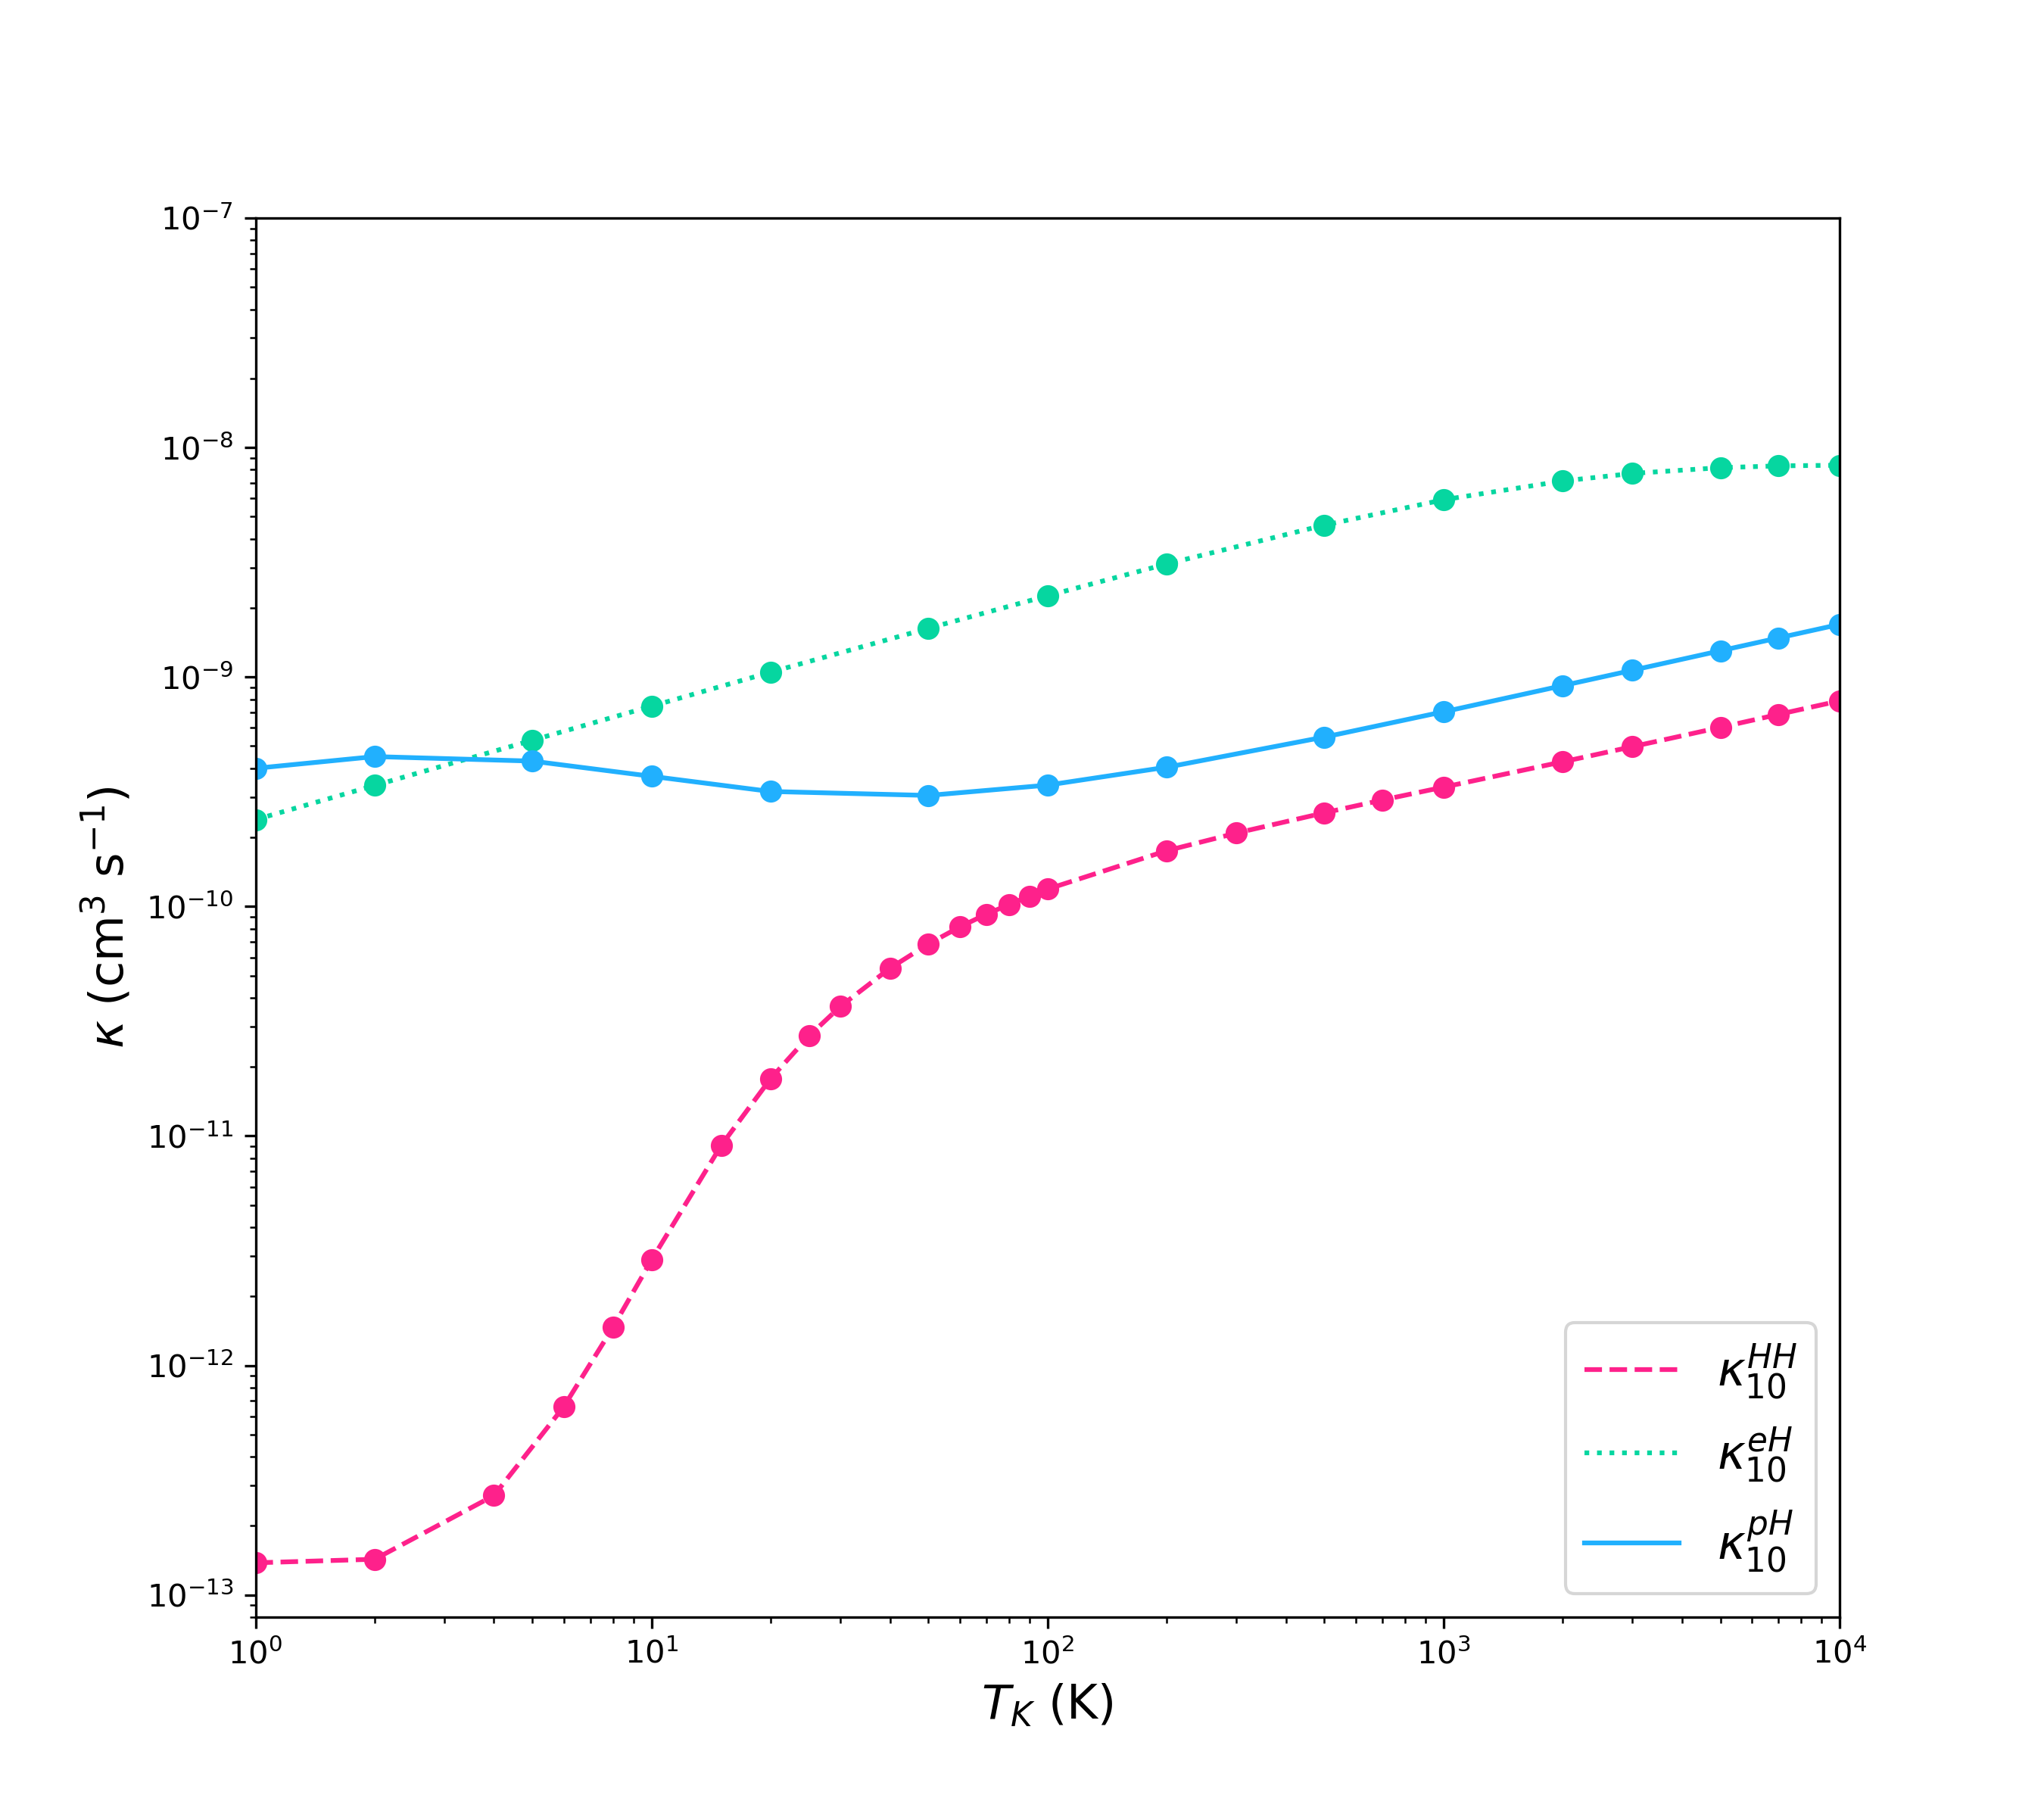
\includegraphics[width=0.99\columnwidth]{figs/collisional_rate.png}
    %\caption{De-excitation rate coefficients for HH collisions (dashed line), eH collisions (dotted line), and pH collisions (solid line). Note that the net rates are also proportional to the densities, so H H collisions still dominate in a weakly ionized medium. (I don't think I need this.)}
    %\label{fig:coll}
%\end{figure}



\subsection{Proper \texorpdfstring{Ly$\alpha$}{Lyman-alpha} intensity}

The Ly$\alpha$ intensity, defined as the angle-averaged number of incident photons hitting a gas element per unit area, time, frequency, and steradian, can be calculated using the following equation:

\begin{equation}
    J^i_\alpha = \frac{(1+z)^2}{4\pi} \sum^{n_\mathrm{max}}_{n=2} f_\mathrm{rec} (n) \int^{z_\mathrm{max}(n)}_z \frac{c \, dz'}{H(z')} \epsilon(\nu'_n, z')\,, \label{eq:Jalpha}
\end{equation}
where $i \in \{{\rm H}, {\rm He}\}$ labels the species, $f_\mathrm{rec} (n)$ is the recycling fraction of photons that redshift into a Ly$n$ resonance and ultimately cascade through the Ly$\alpha$ resonance \citep[][]{Pritchard2007}, $n_\mathrm{max}$ is the maximum Lyman level considered, $z_\mathrm{max}(n)$ is the maximum redshift from which a photon can be emitted without redshifting into the subsequent Ly$(n+1)$ resonance, and $\epsilon(\nu'_n, z')$ is the comoving spectral emissivity of the radiation sources. The emissivity $\epsilon(\nu'_n, z')$ sums over all radiation sources in \lumina. Beyond the stellar populations (Section \ref{sec:stars}), which dominate the soft-UV Ly$\alpha$ background, we include contributions from the hot ISM, HMXBs, and AGN (Section~\ref{sec:others}). These hard-UV and X-ray sources contribute to the Ly$\alpha$ field directly. However, note that we do not include the indirect Ly$\alpha$ produced by collisional excitation from secondary electrons, consistent with our assumption of maximal X-ray heating efficiency ($f_{\rm heat}=1$), which by construction leaves no absorbed X-ray energy in the excitation channel. We discuss the consequences in Section~\ref{sec:xray_heating}.


The emitted frequency, $\nu'_n$, at a higher redshift $z'$ that redshifts into the Ly$n$ resonance at redshift $z$ is given by:

\begin{equation}
    \nu'_n = \nu_\mathrm{LL}^i (1-n^{-2})\frac{1+z'}{1+z}\,,
\end{equation}
where $\nu_\mathrm{LL}$ is the Lyman limit frequency, which corresponds to $3.289 \times 10^{15}\,\mathrm{Hz}$ for neutral hydrogen and $1.316 \times 10^{16}\,\mathrm{Hz}$ for singly ionized helium.


To redshift into a given Ly$n$ resonance at redshift $z$ without first being absorbed by the higher-order Ly$(n+1)$ resonance, a photon must have been emitted at a redshift below the maximum value given by:

\begin{equation}
    1 + z_\mathrm{max}(n) = (1+z) \frac{[1-(n+1)^{-2}]}{1-n^{-2}}\,.
\end{equation}

Therefore, we sum the photon number flux emitted between consecutive atomic levels and integrate over all sources out to the comoving distance corresponding to the appropriate redshift interval. In this work, we consider Lyman transitions up to the $n=30$ energy level.

To evaluate Eq. (\ref{eq:Jalpha}) as a spatially-resolved three-dimensional field, we exploit the fact that for a fixed Lyman-$n$ line and a fixed emission redshift $z'$, the contribution to $J^i_\alpha$ is proportional to the SFRD averaged over a sphere of comoving radius $R(z, z')$ centered on $\mathbf{x}$, where $R$ is the comoving distance between $z$ and $z'$. This sphere-averaged field is computed efficiently via the convolution theorem. We perform a forward Fast Fourier Transform (FFT) of the SFRD box at $z'$, multiply each Fourier mode $k$ by the top-hat window function:

\begin{equation}
    W(kR) = \frac{3\left[\sin(kR) - kR\cos(kR)\right]}{(kR)^3}\,,
    \label{eq:tophat}
\end{equation}
and transform back to real space. The integral over $z'$ is discretized into $N_\mathrm{shells} = 200$ (400 for the AGN contribution) logarithmically spaced radial shells between $R_\mathrm{min}$ (one cell width) and $R_\mathrm{max}(n) = R(z, z_\mathrm{max}(n))$, with the SFR field at each shell midpoint obtained by linearly interpolating between the two bracketing simulation snapshots. This approach, following \citet{Mesinger2011}, reduces the computational cost from $\mathcal{O}(N^6)$ for a direct summation to $\mathcal{O}(N_\mathrm{shells} \cdot N^3 \log N)$, making the calculation tractable on a $640^3$ grid.


Following \citet{Mesinger2011}, we approximate each shell by the SFRD averaged over the full sphere of radius $R$. This preserves the mean of $J^i_\alpha$ exactly but weights nearby emission up to $1.5$ times more heavily than a true shell average, so the local $J^i_\alpha$ changes by much less than this factor wherever distant sources dominate the flux, and by up to this factor only in the immediate vicinity of bright sources. The effect is negligible once the coupling saturates, so for hydrogen it is confined to $z \gtrsim 10$, while for the weakly coupled helium line it is further diluted by the collisional contribution to the coupling.


\subsection{Stellar photon emissivity} \label{sec:stars}
Stellar radiation is the primary driver of \ion{H}{1} reionization. In Eq. (\ref{eq:Jalpha}), $\epsilon(\nu_n, z)$ is the comoving photon emissivity from stars, defined as the number of photons emitted per unit comoving volume, per unit proper time, and per unit frequency, evaluated at the rest-frame frequency $\nu_n$ at the source redshift $z$ \citep[][]{Barkana2001}:

\begin{subequations}
\begin{align}
    \epsilon_\star(\nu,z) & =
    \bar{n}^0_b \,f_\star \,
    \frac{d}{dt}f_\mathrm{coll}(z) \,\epsilon_b(\nu) \label{eq:sub1} \\
    & = \frac{\dot{\rho}_{\star,\mathrm{cell}}}{m_p} \epsilon_b(\nu)\,, \label{eq:sub2}
\end{align}
\end{subequations}
where $\bar{n}^0_b$ is the present-day ($z=0$) cosmic mean baryon number density, $f_\star$ is the star formation efficiency within galactic halos, and $f_\mathrm{coll}(z)$ is the collapsed gas fraction in galaxies at redshift $z$.


Within the \lumina framework, the term $\bar{n}^0_b f_\star df_\mathrm{coll}(z)/dt$ is intrinsically equivalent to the star formation rate density (SFRD) $\dot{\rho}_{\star,\mathrm{cell}}$, which we extract directly from the simulation snapshots or global data as Eq. (\ref{eq:sub2}). This contrasts with semi-analytic approaches that must compute $f_\mathrm{coll}$ by integrating over a theoretical halo mass function \citep[e.g.][]{Barkana2005, Kaurov2016, Mesinger2011} in Eq. (\ref{eq:sub1}).

The term $\epsilon_b(\nu)$ characterizes the intrinsic spectral energy distribution (SED) of the stellar radiation sources, representing the number of emitted photons at frequency $\nu$ per baryon incorporated into stars. We use the same BPASS SEDs as in the on-the-fly radiative transfer of \lumina, with the minimum and maximum stellar masses set to $0.1~\mathrm{M}_\odot$ and $100~\mathrm{M}_\odot$, respectively. BPASS tabulates the SED at 13 metallicities ($Z = 10^{-5}\text{--}0.04$). In the Lyman-series integral, $\epsilon_b$ is evaluated at the mass-weighted mean metallicity of all \lumina star particles at the emission redshift $z'$, and the same value is applied to every cell. We interpolate $\epsilon_b$ linearly in $\log Z$ between adjacent tabulated values and adopt $Z = 10^{-5}$ when the mean metallicity falls below this range, as at the highest redshifts, where the stars are nearly metal-free. We refer to this choice as the fiducial model and test its sensitivity to the adopted metallicity in Appendix~\ref{sec:metallicity}.


No escape fraction is applied to $\epsilon_b(\nu)$ in Equation~(\ref{eq:sub2}), for either the \ion{H}{1} or the \ion{He}{2} Lyman band. The Lyman-band continuum that sets $J_\alpha^\mathrm{H}$ lies between Ly$\alpha$ and the Lyman limit ($10.2\text{--}13.6$\,eV), below the \ion{H}{1} ionization threshold, so it is not subject to the photoelectric absorption by host-ISM \ion{H}{1} that suppresses the ionizing output. The stellar escape fraction $f_\mathrm{esc,\star} = 0.18$ of Section~\ref{sec:rt} applies only to the ionizing ($>13.6$\,eV) output and does not enter Equation~(\ref{eq:sub2}). Following standard practice in Ly$\alpha$ background modeling \citep[e.g.][]{Barkana2005, Mesinger2011}, we neglect the remaining host-galaxy losses in this band, such as dust and absorption in the damped wings of the Lyman-series lines. These would lower $J_\alpha^\mathrm{H}$ by a modest factor but have little effect on $\delta T_b^\mathrm{H}$ once $x_\alpha^\mathrm{H} \gg 1$ (Appendix~\ref{sec:metallicity}).


The \ion{He}{2} Lyman band ($40.8\text{--}54.4$\,eV) requires more care. It lies above the \ion{H}{1} and \ion{He}{1} ionization thresholds and is therefore absorbed in both the host ISM and the IGM, neither of which is included in Equation~(\ref{eq:Jalpha}). For stars, this is equivalent to $f_\mathrm{esc} = 1$, whereas the radiative transfer applies the frequency-independent $f_\mathrm{esc,\star} = 0.18$ at $z > 4.75$ \citep{Zier2026}. The true value should lie between the two. The combined \ion{H}{1} and \ion{He}{1} opacity per hydrogen atom is $12\text{--}25$ times lower than at the Lyman limit \citep{Verner1996}, but typical host columns ($N_\mathrm{HI} \gtrsim 10^{20}\,\mathrm{cm^{-2}}$) remain optically thick. If photons escape mainly through low-column channels, the escape fraction stays close to $0.18$. Host absorption alone may therefore lower the stellar contribution by up to $1/0.18 \approx 5.6$. For AGN, the emissivity already includes the luminosity-dependent escape fraction of \lumina, $f_\mathrm{esc}^\mathrm{AGN} = 0.3\,(L_\mathrm{bol}/10^{46}\,\mathrm{erg\,s^{-1}})^{0.07} \approx 0.2\text{--}0.35$ \citep{Zier2026, Shen2026a}, so no further factor is applied.

Absorption in the IGM lowers both components further. It is modest after overlap but severe while neutral islands remain ($z \gtrsim 5.5$), where the mean free path in this band is only $\sim 10$ proper kpc. Our $J_\alpha^\mathrm{He}$ is therefore an upper limit on the transported background for the adopted emissivities. Because the $^3$He$^+$ line is weakly coupled, $\delta T_b^\mathrm{He}$ responds to this uncertainty in proportion to the radiative share of the coupling, $x_\alpha/(x_\alpha + x_c)$. We also omit local \ion{He}{2} Ly$\alpha$ production from \ion{He}{3} recombination cascades and secondary-electron excitation, which would add photons beyond this limit.


\subsection{Other X-ray and hard-UV sources} \label{sec:others}


While soft stellar UV radiation dominates the Ly$\alpha$ flux and the ionization history at $z \gtrsim 10$, X-ray heating and harder, non-stellar UV emission become increasingly important as the Universe evolves toward $z \sim 3$. Beyond primary stellar UV, these populations can contribute to the Ly$\alpha$ background through direct UV emission, recombination radiation in partially ionized regions, and collisional excitation by the secondary electrons produced in X-ray photoionization \citep{Madau1997}. We include only their direct emission, which is small compared with the stellar contribution. Their main effect on the hyperfine signals is through X-ray heating, which raises the kinetic temperature $T_K$ through Coulomb collisions. These high-energy components govern the thermal transition of the IGM and the extended tail of reionization, and are essential for both the 21\,cm and the 3.46\,cm signals.


To capture this budget self-consistently, \lumina models three high-energy source populations: the hot interstellar medium (ISM), high-mass X-ray binaries (HMXBs), and active galactic nuclei (AGN). The hot ISM and HMXBs scale with the star formation rate, while AGN scale with the black hole accretion rate. All three are unified within a single radiative transport framework, with the resulting Ly$\alpha$ intensity $J_\alpha$ computed by the same lightcone integration used for the stellar background (Equation \ref{eq:Jalpha}),  summing the emissivity $\epsilon$ over all contributing populations. We note, however, that the early Ly$\alpha$ and X-ray backgrounds at $z \gtrsim 10$ are subject to several physical uncertainties. These include the limited mass resolution of \lumina (which prevents the direct resolution of minihalos), the absence of a Population III (Pop III) stellar model, and sparse observational constraints on the early star formation rate density. We discuss the implications of these limitations in Section \ref{sec:highz}.


A complete description of the SED construction, luminosity calibration, and radiative transport of these fields is presented in \citet{Zier2026}; here we summarize the ingredients relevant to our $J_\alpha$, 21\,cm, and 3.46\,cm predictions.


%Beyond primary stellar UV, these populations build a Ly$\alpha$ emission through several channels: direct UV emission from quasars, recombination radiation in partially ionized regions, and collisional excitation by the secondary electrons produced in X-ray photoionization \citep{Madau1997}. The X-ray fields in \lumina therefore play a dual role: they heat the IGM by raising the kinetic temperature $T_K$ through Coulomb collisions, and they enhance the Wouthuysen--Field coupling coefficient $x_\alpha$.




\subsubsection{Hot ISM}


The shock-heated diffuse ISM is modeled with a thermal bremsstrahlung spectrum, normalized using the empirical $L_X$--SFR relation of \citet{Mineo2012}. We adopt the luminosity normalization $L^{10\text{-}2000\,\mathrm{eV}}[\mathrm{erg \ s^{-1}}]= 3.3 \times 10^{40}\,\left[\mathrm{SFR}/M_\odot\ \mathrm{yr}^{-1}\right]$, and inject the corresponding emission per voxel according to its local SFR, in direct analogy with the stellar Ly$\alpha$ treatment.


\subsubsection{HMXBs}
For HMXBs, we adopt the intrinsic SEDs of \citet{Fragos2013, Fragos2016}. The integrated luminosity depends on both metallicity and the local SFR; we use the parametrization of \citet{Madau2017} and convert their values to our reference band, $L^{10\text{-}2000\,\mathrm{eV}}_{\mathrm{HMXB}}$.

\subsubsection{Black holes}

AGN provide hard ionizing radiation and are the dominant contributors to \ion{He}{2} reionization. We adopt the composite quasar SED of \citet{Shen2020}. For each active black hole, the intrinsic luminosity is $L^{\mathrm{AGN}}_{\mathrm{bol}} = \epsilon_{\mathrm{rad}}\,(1 - \epsilon_{f,\mathrm{high}})\,\dot{M}_{\mathrm{BH}}\,c^2$, where the factor $(1 - \epsilon_{f,\mathrm{high}})$ removes the fraction of the radiated output thermally coupled to the gas as high-accretion (quasar-mode) feedback, leaving the luminosity available for radiative transport. We further apply a luminosity-dependent obscuration correction for unresolved gas and dust following \citet{Hopkins2007} and \citet{Vogelsberger2013}. The resulting AGN luminosities are deposited on the Cartesian grid and smoothed over the corresponding comoving distance to account for radiative transport.



%\section{Cosmic Variance Example (VID)}

%\textcolor{red}{Possible modification needed: VID section, Discussion (Large-Scale Volume)}


\section{Sensitivity to the stellar spectral model} \label{sec:metallicity}


\begin{figure}[!t]
    \centering
    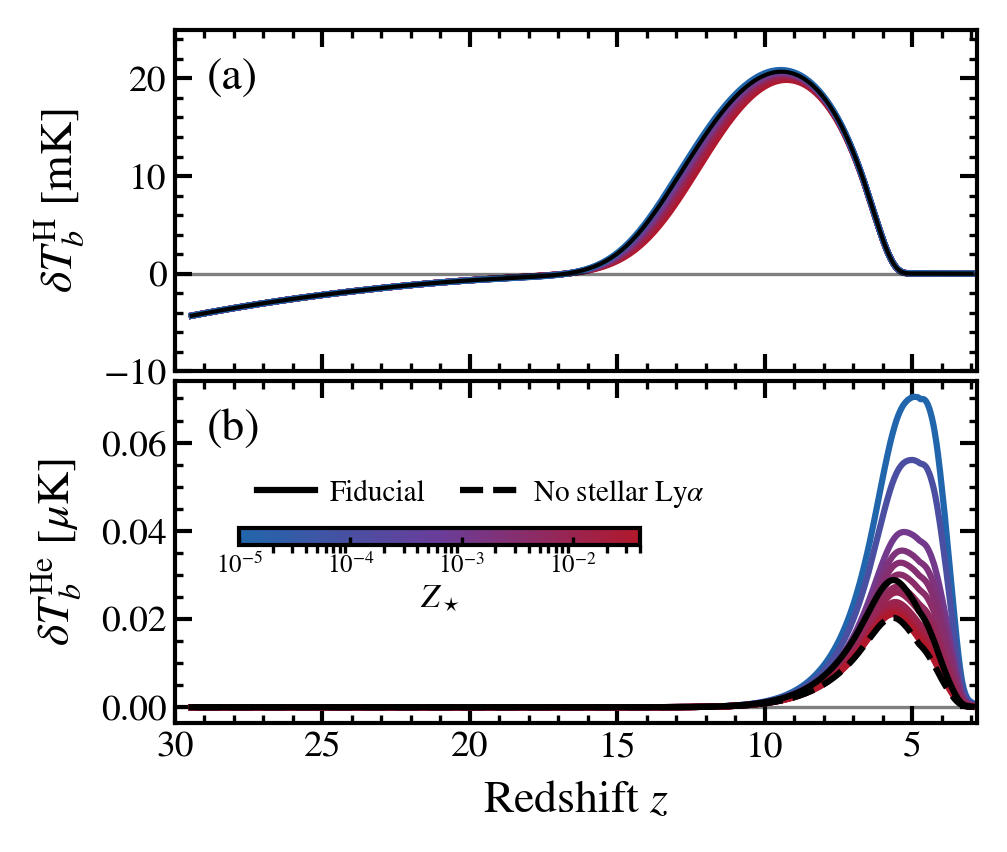
\includegraphics[width=\linewidth]{figs/metallicity.png}
    \caption{Sensitivity of global brightness temperatures to the stellar metallicity adopted for the Ly$\alpha$ emissivity. Colored curves show all 13 BPASS v2.2.1 metallicities ($Z_\star = 10^{-5}\text{--}0.04$, blue to red), with the gas ionization and thermal state held fixed to the \lumina simulation output. The black solid curve shows the fiducial model, in which the metallicity at each redshift is set to the mass-weighted mean metallicity of the \lumina star particles at that redshift. The black dashed curve in panel~(b) excludes the stellar Ly$\alpha$ background, retaining only AGN radiation and collisional coupling. (a) 21\,cm differential brightness temperature $\delta T_\mathrm{b}^\mathrm{H}$. (b) 3.46\,cm brightness temperature $\delta T_\mathrm{b}^\mathrm{He}$.}
    \label{fig:metallicity}
\end{figure}

Our fiducial model evaluates the BPASS emissivity $\epsilon_b$ at the mean metallicity of the \lumina star particles (Appendix~\ref{sec:stars}). A single mean does not capture the spread of stellar metallicities at a given redshift, so we recompute $J_\alpha^\mathrm{H}$ and $J_\alpha^\mathrm{He}$ for each of the 13 BPASS v2.2.1 metallicities ($Z = 10^{-5}\text{--}0.04$), each applied at all redshifts, while holding the gas ionization and thermal state fixed to the simulation output. Differences among these models isolate the effect of Ly$\alpha$ background intensity on the spin temperature, and thus on the resulting differential brightness temperature, as shown in Figure~\ref{fig:metallicity}.

The 21\,cm signal is only weakly affected, with the emission peak varying by $\approx 6$\% across the full metallicity range and metal-poor populations producing marginally stronger emission. This insensitivity reflects the saturation of Wouthuysen--Field coupling during the EoR. Once $x_\alpha^\mathrm{H} \gg 1$, $T_S^\mathrm{H}$ becomes locked to $T_K$, rendering further changes in Lyman-band emissivity largely inconsequential for $\delta T_b^\mathrm{H}$. The hydrogen predictions presented in this work are therefore robust against the assumed stellar metallicity.

The 3.46\,cm signal behaves differently, as its peak amplitude decreases by a factor of $\approx 3$ from $Z = 10^{-5}$ to $Z = 0.04$. Over $z \approx 3\text{--}6$, where the helium signal peaks, the mean stellar metallicity rises from $\approx 5\times10^{-3}$ at $z \approx 6$ to $\approx 0.016$ at $z \approx 3$, so the fiducial amplitude lies toward the lower end of this range. Two compounding effects drive the metallicity dependence. First, the \ion{He}{2} Lyman band ($40.8\text{--}54.4$\,eV) lies on the steeply falling high-energy tail of the stellar spectrum, where continuum output depends strongly on the effective temperatures of the most massive stars and, by extension, on metallicity. Thus, $J_\alpha^\mathrm{He}$ is far more sensitive to $Z$ than $J_\alpha^\mathrm{H}$. Second, the \ion{He}{2} hyperfine transition remains weakly coupled throughout, maintaining $T_S^\mathrm{He}$ close to $T_\gamma$ (Figure~\ref{fig:global}(a)). In this weakly coupled regime, $\delta T_\mathrm{b}^\mathrm{He}$ scales linearly with $x_\alpha^\mathrm{He}$ instead of saturating. In short, the contrast between hydrogen and helium reflects a transition between saturated and linear coupling physics.

Two caveats apply to the helium amplitude. First, the amplitude of $\delta T_\mathrm{b}^\mathrm{He}$ in \lumina is governed by comparable radiative and collisional contributions, so its radiative part inherits the physical uncertainties of the high-energy stellar spectrum. Second, and more importantly, the $J_\alpha^\mathrm{He}$ entering this calculation is unattenuated and represents a an upper limit on the transported background for the adopted emissivities (Appendix~\ref{sec:stars}). Continuum absorption of the \ion{He}{2} Lyman band in the host ISM and IGM would lower the helium amplitude for every metallicity.

The spread in Figure~\ref{fig:metallicity} thus isolates sensitivity to the stellar spectrum in the absence of attenuation rather than the full uncertainty on the 3.46\,cm amplitude. Stars dominate this band: at $z \approx 5$, their \ion{He}{2} Lyman-band emissivity exceeds that of AGN by a factor of a few, whereas AGN dominate above the $54.4$\,eV ionization threshold \citep[][their Fig.~19]{Zier2026}. While AGN drive \ion{He}{2} reionization, they supply only a minority of the helium Lyman-series photons that set the Wouthuysen--Field coupling of the 3.46\,cm line. AGN emission and collisions establish a metallicity-independent baseline for the coupling, setting a floor on $\delta T_b^\mathrm{He}$ (black dashed curve). This floor compresses the signal variance at high $Z$, where stellar spectra soften. Although AGN can dominate the coupling locally around their hosts, their volume-averaged radiative contribution to the global signal is therefore smaller than both the stellar and the collisional contributions.

\end{appendix}





\end{document}
